% ============ \emph{平展上同调讲义}中文翻译 LaTeX 重排版 ============
% 原书: J.S. Milne, Lectures on Étale Cohomology (v2.21, March 22, 2013)
% 模板: AJbook.cls (李文威\emph{代数学方法}书系模板)
%       ★ 定理编号规则已按原书修改(见 AJbook.cls): 定理/推论/引理/命题/定义/
%         例/注记/附记/问题/习题/注意 共享一个计数器, 按章(原书小节)编号
% 结构: 记号与约定 + 预备知识与参考文献 + 致谢 + 评注
%       + 第一部分 基本理论(§1-25) + 第二部分 Weil 猜想的证明(§26-34) + 索引
%
% 编号体系 (原书约定):
%   - 章 = 原书小节: 1-34 连续阿拉伯编号 (跨两部分,
%     \counterwithout{chapter}{part} + \renewcommand{\AJchapterttl})
%   - 定理类: 共享计数器, 编号 N.M 与原书一致 (如 命题 2.1, 注记 2.3, 附记 3.6)
%   - 公式: 原书绝大多数不编号, 少数按局部编号, 用显式 \tag{...}
\documentclass[geometry=a4, fontsetup=font-setup-open.tex, titlesetup=titles-setup, coverpage=cover, CJKthechapter=false]{AJbook}

% ============ 宏包 ============
\usepackage{mycommand}      % 常用数学命令(\dd \R \Z \Q \CC \e \ii \Spec \Gm \Gal 等)
\usepackage{myarrows}       % 可伸缩箭头
\usepackage{amssymb}
\usepackage{chngcntr}       % \counterwithout
\usepackage{tikz-cd}        % 交换图
\usepackage{imakeidx}
\usepackage[bookmarksnumbered=true]{hyperref}
\usetikzlibrary{calc}       % 封面坐标计算

% ============ 编号体系 ============
\counterwithout{chapter}{part}                  % 章(原书小节)编号 1-34 跨两部分连续
\renewcommand{\AJchapterttl}[1]{#1}             % 章号显示为阿拉伯数字(与原书 "1 Introduction" 一致)

% 天眉: "2 平展态射". AJbook.cls 在 \AtBeginDocument 里定义 \chaptermark, 故此处覆盖须放在其之后
\AtBeginDocument{%
  \renewcommand{\chaptermark}[1]{\markboth{\thechapter\quad #1}{}}%
}

% ============ 超链接 ============
\hypersetup{
    pdfauthor={J.S. Milne},
    pdftitle={平展上同调讲义 (Lectures on Étale Cohomology)},
    pdfsubject={代数几何},
    colorlinks=true,
    linkcolor=MidnightBlue,
    citecolor=BrickRed,
    urlcolor=MidnightBlue
}

% ============ 自定义命令 ============
\newcommand{\Specm}{\operatorname{Specm}}       % 极大谱
\newcommand{\Tgt}{\operatorname{Tgt}}           % 切空间/切锥
\newcommand{\OX}{\mathcal{O}_X}                 % 结构层
\newcommand{\Fbar}{\overline{\mathcal{F}}}
\newcommand{\Qell}{\mathbb{Q}_{\ell}}           % ℓ 进数域
\newcommand{\Zell}{\mathbb{Z}_{\ell}}           % ℓ 进整数环
\newcommand{\etale}{平展}                        % (备用, 直接写中文亦可)

% 索引 (intoc=false: 目录条目由 titlesec 无号章 after-code 添加, 避免重复)
\makeindex[columns=2, intoc=false, title={索引}]

% 全局断行弹性: 消除边界性 Overfull (与 Gelbart/古典调和分析项目同款)
\emergencystretch=3em

% ============ 文档开始 ============
\begin{document}
\frontmatter        % 封面(cover.tex) + 目录(模板自动处理, 罗马页码)

% 前言部分 (原书 pp.4-6)
% ============ 前言部分 (原书 pp.4-6) ============
% 记号与约定 / 预备知识与参考文献 / 致谢 / 评注
% (原书目录不收录这些条目, 故用 \chapter* 不加入目录)

\chapter*{记号与约定}

关于簇的约定与我的\emph{代数几何}讲义中的相同.例如，域 $k$ 上的仿射代数(affine algebra)是有限生成的 $k$-代数 $A$，使得对 $k$ 的一个(从而每个)代数闭包 $k^{\mathrm{al}}$，$A \otimes_k k^{\mathrm{al}}$ 无非零幂零元---这蕴含 $A$ 本身无幂零元.对这样的 $k$-代数，我们联系一个环化空间 $\operatorname{Specm}(A)$(赋予 $k$-代数层结构的拓扑空间)，而 $k$ 上的仿射簇是同构于这种形式的环化空间.$k$ 上的簇是环化空间 $(X, \mathcal{O}_X)$，它有一个有限开覆盖 $X = \bigcup U_i$，使得每个 $(U_i, \mathcal{O}_X|_{U_i})$ 都是仿射簇，并且满足分离公理.我们常用 $X$ 同时表示 $(X, \mathcal{O}_X)$ 及其底层拓扑空间.簇的正则映射有时也称为簇的态射.

对偏好概形的读者：簇是域 $k$ 上有限型的分离，几何既约概形 $X$，其中非闭点被去掉.

若 $X$ 是 $k$ 上的簇，$K \supset k$，则 $X(K)$ 是 $X$ 中坐标在 $K$ 里的点的集合，而 $X_K$ 或 $X_{/K}$ 是由 $X$ 得到的 $K$ 上簇\footnote{我们的术语遵循 Grothendieck.存在一种相冲突的术语，基于 Weil 的 \emph{Foundations}，常被代数群理论的研究者使用，它把两者反过来写.}.例如，若 $X = \operatorname{Specm}(A)$，则 $X(K) = \operatorname{Hom}_{k\text{-alg}}(A, K)$，且 $X_K = \operatorname{Specm}(A \otimes_k K)$.一般地，$X(K)$ 只是一个集合，但我通常赋予 $X(\mathbb{C})$ 自然的复拓扑.域 $k$ 的可分闭包 $k^{\mathrm{sep}}$ 是 $k$ 的代数扩张，使得每个系数在 $k$ 中的可分多项式在 $k^{\mathrm{sep}}$ 中都有根.

关于概形的术语是标准的，只有一点除外：我总假定我们的环是 Noether 的，我们的概形是局部 Noether 的.

关于环的术语是标准的.特别地，环的同态 $A \to B$ 把 1 映到 1.环同态 $A \to B$ 是有限的，而 $B$ 是有限 $A$-代数，如果 $B$ 作为 $A$-模有限生成.当 $A$ 是局部环时，我常用 $\mathfrak{m}_A$ 记其(唯一的)极大理想.局部环的局部同态是同态 $f \colon A \to B$，使得 $f^{-1}(\mathfrak{m}_B) = \mathfrak{m}_A$(等价地，$f(\mathfrak{m}_A) \subset \mathfrak{m}_B$).

一般地，当我从拓扑空间上的层论汲取动机时，我假定空间是 Hausdorff 的，即不是那种有点的闭包为全空间的怪空间.

\begin{itemize}
  \item $X \subset Y$：$X$ 是 $Y$ 的子集(不一定是真子集);
  \item $X \overset{\mathrm{def}}{=} Y$：$X$ 定义为 $Y$，或按定义等于 $Y$；
  \item $X \cong Y$：$X$ 同构于 $Y$；
  \item $X \approx Y$：$X$ 与 $Y$ 典范同构(或存在给定的或唯一的同构).
\end{itemize}

\chapter*{预备知识与参考文献}

\textbf{同调代数} 我假定读者熟悉 Abel 范畴与导出函子的语言.这些主题在我的\emph{类域论}讲义 pp.69--76 中有概述，若干书中有完整叙述，例如
\begin{quote}
  Weibel, C.A., \emph{An Introduction to Homological Algebra}\footnote{在第 9 页，Weibel 定义 $C[p]_n = C_{n-p}$.正确的原始定义(代数几何学家与算术几何学家普遍使用)是 $C[p]_n = C_{n+p}$(见 Hartshorne, R., \emph{Residues and Duality}, 1966, p.26).此外，在 Weibel 中，``函子范畴''不一定是范畴.}, Cambridge U.P., 1994.
\end{quote}
我们不能避免使用谱序列---谱序列的简短概述见我的\emph{平展上同调}一书 pp.307--309，完整处理见 Weibel 的书第 5 章.

\textbf{层论} 平展上同调以通常拓扑意义下的层上同调理论为模型.本讲义中的许多材料与例如下面的材料平行：
\begin{quote}
  Iversen, B., \emph{Cohomology of Sheaves}, Springer, 1986.
\end{quote}

\textbf{代数几何} 我假定读者熟悉代数簇的理论，例如我的\emph{代数几何}讲义(Math. 631).此外，有时我会提到概形，因此读者应熟悉概形的基本语言，例如 Hartshorne, \emph{Algebraic Geometry}, Springer 1977 第 II 章的前 3 节，Eisenbud and Harris, \emph{Schemes}, Wadsworth, 1992 的第 1 章，或 Shafarevich, \emph{Basic Algebraic Geometry}, 2nd Edition, Springer, 1994 的第 V 章.

交换代数我通常参考
\begin{quote}
  Atiyah, M., and MacDonald, I., \emph{Introduction to Commutative Algebra}, Addison-Wesley, 1969.
\end{quote}

\textbf{平展上同调} 有下列书籍：
\begin{quote}
  Freitag, E., and Kiehl, R., \emph{Etale Cohomology and the Weil Conjecture}, Springer, 1988.\\
  Milne, J., \emph{Etale Cohomology}, Princeton U.P. 1980 (引用为 EC).\\
  Tamme, \emph{Introduction to Etale Cohomology}, Springer.
\end{quote}

原始文献：
\begin{quote}
  Artin, M., \emph{Grothendieck Topologies}, Lecture Notes, Harvard University Math. Dept. 1962.\\
  Artin, M., \emph{Th\'eor\`emes de Repr\'esentabilit\'e pour les Espaces Alg\'ebriques}, Presses de l'Universit\'e de Montr\'eal, Montr\'eal, 1973\\
  Grothendieck, A., et al., \emph{S\'eminaire de G\'eom\'etrie Alg\'ebrique}.\\
  SGA 4 (with Artin, M., and Verdier, J.-L.). \emph{Th\'eorie des topos et cohomologie \'etale des sch\'emas} (1963--64). Springer Lecture Notes 1972--73.\\
  SGA $4\frac{1}{2}$ (by Deligne, P., with Boutot, J.-F., Illusie, L., and Verdier, J.-L.) \emph{Cohomologie \'etale}. Springer Lecture Notes 1977.\\
  SGA 5 \emph{Cohomologie l-adique et fonctions L} (1965--66). Springer Lecture Notes 1977.\\
  SGA 7 (with Deligne, P., and Katz, N.) \emph{Groupes de monodromie en g\'eom\'etrie alg\'ebriques} (1967--68). Springer Lecture Notes 1972--73.
\end{quote}

除 SGA $4\frac{1}{2}$ 外，这些都是 Grothendieck 在 I.H.E.S. 领导的著名讨论班.

我引用我的如下讲义.
\begin{quote}
  FT \emph{Field and Galois Theory} (v4.40 2013).\\
  AG \emph{Algebraic Geometry} (v5.22 2012).\\
  AV \emph{Abelian Varieties} (v2.00 2008).\\
  CFT \emph{Class Field Theory} (v4.01 2011).
\end{quote}

\chapter*{致谢}

我感谢以下人士为这些讲义的早期版本提供勘误与意见：Martin Bright; Rex Cheung; Sungmun Cho; Ming-chang Kang; Michiel Kosters; Akhil Matthew; Carl Mautner and others at UT Austin; Behrooz Mirzaii; Eric Moorhouse; Sean Rostami; Steven Spallone; Immanuel Stampfli; Sun Shenghao; Zach Teitler; Bhupendra Nath Tiwar; Ravi Vakil.

\chapter*{评注}

平展上同调中的主要定理都在 SGA 4 和 SGA 5 中证明，但常常是在不必要地严格的假设之下.其中一些假设后来被去除了，但所用的证明大量使用了那些讨论班的内容.因此这门学科的结构需要重新思考.此外，代数空间应当更充分地融入这门学科(见 Artin 1973).de Jong 的分解定理(\emph{Smoothness, semi-stability and alterations}. Inst. Hautes \'Etudes Sci. Publ. Math. No. 83 (1996), 51--93)很可能允许许多改进.最后，诸如相交上同调与 Borel-Moore 同调这样的主题需要补充到讲述中.这些都不会在这份讲义中尝试.

\begin{quote}
  我认为，Grothendieck 在 1958 年 Serre 于 Chevalley 讨论班上的报告之后之所以确信平展局部化会给出正确的 $H^i$，是因为一旦你有了曲线的正确上同调，那么通过曲线纤维化与 d\'evissage，你也应当能达到更高的 $H^i$.(Illusie, NAMS 2010.)
\end{quote}

\begin{quote}
  Grothendieck 第一次来哈佛是在 1958 年.Artin：是的.那时我还不知道概形是什么.但第二次，在 '61 年，我听说他有平展上同调的想法，当他到达时我问他我是否可以思考它，那就是开始.他当时并没有在做这个---他有这个想法但把它搁置了.他直到我证明了第一个定理才开始做它.他极其活跃，但在那些年里，这可能是他唯一一件没有立刻做的事，原因不明.那年秋天我思考了它，我们争论定义应该是什么[笑].然后我在 '62 年秋天做了一个讨论班.(\emph{Recountings: conversations with MIT mathematicians}, p.358.)
\end{quote}


\mainmatter         % 正文(阿拉伯页码从 1 开始)

\part{基本理论}
\setcounter{footnote}{0}    % 脚注在每部分内连续编号(与原书一致: 第一部分 1-10+)
% ============ 1 引言 (原书 pp.7-15) ============
\chapter{引言}\label{sec:1}
\index{平展上同调}
\index{Betti 数}
\index{代数拓扑}
\index{层上同调}
\index{Zariski 拓扑}
\index{平展态射}
\index{比较定理}

对复数域上的簇 $X$，$X(\mathbb{C})$ 从 $\mathbb{C}$ 获得一个拓扑，因此可以把代数拓扑的机器用于它的研究.例如，可以定义 $X$ 的 Betti 数 $\beta_r(X)$ 为向量空间 $H^{r}(X(\mathbb{C}), \mathbb{Q})$ 的维数，并且诸如 Lefschetz 不动点公式之类的定理都是可用的.

对任意代数闭域 $k$ 上的簇 $X$，只有 Zariski 拓扑，它太粗糙(即开子集太少)，以至于代数拓扑的方法无法使用.例如，若 $X$ 不可约，则用 Zariski 拓扑计算的群 $H^{r}(X, \mathbb{Z})$ 对一切 $r > 0$ 都为零.

在 1940 年代，Weil 观察到，他在有限域上某些簇(曲线，阿贝尔簇，对角超曲面等)的点数方面的某些结果，可以用一种上同调理论的存在性来解释：该理论给出特征零域上的向量空间，并且对这种理论 Lefschetz 不动点公式成立.他的结果预测了 $\mathbb{C}$ 上 $\mathbb{P}^{d+1}$ 中对角超曲面的 Betti 数公式，后来被 Dolbeault 验证.

大约在 1958 年，Grothendieck 定义了概形的平展``拓扑''，平展上同调理论由他在 M. Artin 和 J.-L. Verdier 的协助下建立.整个理论紧密模仿拓扑空间上通常的层论及其导出函子上同调.对 $\mathbb{C}$ 上的簇 $X$，当 $\Lambda$ 是有限群，$\ell$ 进整数环 $\mathbb{Z}_{\ell}$ 或 $\ell$ 进数域 $\mathbb{Q}_{\ell}$ 时(但对 $\Lambda = \mathbb{Z}$ 不成立)，平展上同调群 $H^{r}(X_{\mathrm{et}}, \Lambda)$ 与复群 $H^{r}(X(\mathbb{C}), \Lambda)$ 一致.当 $X$ 是域 $K$ 的谱时，$X$ 的平展上同调理论恰与 $K$ 的 Galois 上同调理论一致.因此，平展上同调弥合了第一种情形(纯几何的)与第二种情形(纯算术的)之间的鸿沟.

正如我们将在课程中看到的，平展上同调确实给出预期的 Betti 数.此外，它满足 Eilenberg-Steenrod 公理的类比，Poincar\'e 对偶定理，Lefschetz 不动点公式，Leray 谱序列等等.Goresky 和 MacPherson 的相交上同调有平展类比，它为奇异簇提供 Poincar\'e 对偶定理.平展上同调在解释 Weil 的观察方面取得了辉煌的成功.

\subsection*{代数拓扑}

我们简要回顾平展上同调所模仿的理论的起源.

代数拓扑起源于 19 世纪末 Riemann,Betti 和 Poincar\'e 关于``同调数''的工作.在 Emmy Noether 的一个观察之后，焦点转向``同调群''.到 1950 年代，已有若干种给拓扑空间配备(上)同调群的方法，例如 Veblen,Alexander 和 Lefschetz 的奇异同调群，Lefschetz 的相对同调群，Vietoris 同调群，\v{C}ech 同调群，以及 Alexander 上同调群.

Eilenberg 和 Steenrod 1953\footnote{\emph{Foundations of Algebraic Topology}, Princeton.}极大地澄清了这种局面，他们证明：对任意``容许的''拓扑空间对范畴，恰好存在一种上同调理论，满足一组简短的公理.考虑例如这样的范畴：对象是空间对 $(X, Z)$，其中 $X$ 是局部紧拓扑空间，$Z$ 是 $X$ 的闭子集，态射是空间对的连续映射.此范畴上的上同调理论是一个反变函子，它给每个空间对配上一列 Abel 群与映射
\[
\cdots \to H^{r-1}(U) \to H^{r}_{Z}(X) \to H^{r}(X) \to H^{r}(U) \to \cdots, \qquad U = X \setminus Z,
\]
满足下列公理：
\begin{enumerate}
  \item (正合性公理) 上述序列正合；
  \item (同伦公理) 映射 $f^{*}$ 只依赖于 $f$ 的同伦类；
  \item (切除) 若 $V$ 在 $X$ 中开且其闭包与 $Z$ 不相交，则包含映射 $(X \setminus V, Z) \to (X, Z)$ 诱导同构 $H^{r}_{Z}(X) \to H^{r}_{Z}(X \setminus V)$；
  \item (维数公理) 若 $X$ 由单点构成，则 $H^{r}(P) = 0$ ($r \neq 0$).
\end{enumerate}
拓扑学家通常把群 $H^{r}_{Z}(X)$ 写为 $H^{r}(X, U)$.同调理论的公理与上述类似，只是所有箭头的方向都反转.若 $(X, Z) \mapsto H^{r}_{Z}(X)$ 是上同调理论，使得 $H^{r}_{Z}(X)$ 是局部紧 Abel 群(例如离散的或紧的)，则 $(X, Z) \mapsto H^{r}_{Z}(X)^{\vee}$ (Pontryagin 对偶)是同调理论.在这种方法中，隐含地只有一个系数群.

在 1940 年代，Leray 试图理解两个空间 $X$ 与 $Y$ 的上同调群之间的关系，其间给定了连续映射 $Y \to X$.这引导他引入层(系数群的局部系统)，层上同调和谱序列(几乎同时 Roger Lyndon 也独立地做着类似的事，他试图理解群 $G$，正规子群 $N$ 与商群 $G/N$ 的上同调之间的关系).

导出函子在 Cartan 和 Eilenberg 1956\footnote{\emph{Homological Algebra}, Princeton.}中被系统地使用，而 Eilenberg 的学生 Buchsbaum 在 1955 年的博士论文中定义了 Abel 范畴的概念，并把 Cartan-Eilenberg 的导出函子理论推广到这种范畴.(``abelian category'' 这个名称归功于 Grothendieck.)

最后，Grothendieck 在他著名的 1957 年 T\^ohoku 论文\footnote{\emph{Sur quelques points d'alg\`ebre homologique}, T\^ohoku Math. J. 9, 119--221.}中证明，拓扑空间上的 Abel 群层范畴是具有足够内射对象的 Abel 范畴，因此可以把空间 $X$ 上的层上同调群定义为如下函子的右导出函子：该函子把层映到其整体截面组成的 Abel 群.固定系数群 $\Lambda$ 的上同调，由它定义的常值层的上同调恢复.这现在是上同调群公认的定义，也是我们定义平展上同调群所采用的方法.我们不固定系数群并为了刻画上同调群而必须考虑所有(容许的)拓扑空间对，而是固定拓扑空间，但考虑该空间上的所有层.

\subsection*{层上同调简述}

设 $X$ 是拓扑空间.我们把 $X$ 的开子集做成一个范畴，其态射只有包含映射，并定义预层为从该范畴到 Abel 群范畴 $\mathbf{Ab}$ 的反变函子.于是，这样的预层 $\mathcal{F}$ 给 $X$ 的每个开子集 $U$ 配上一个 Abel 群 $\mathcal{F}(U)$，给每个包含 $V \subset U$ 配上限制映射 $\rho^{U}_{V} \colon \mathcal{F}(U) \to \mathcal{F}(V)$，使得 $\rho^{U}_{U} = \mathrm{id}_{\mathcal{F}(U)}$，并且每当 $W \subset V \subset U$ 时
\[
\rho^{U}_{W} = \rho^{V}_{W} \circ \rho^{U}_{V}.
\]
由于历史原因，$\mathcal{F}(U)$ 的元素称为 $\mathcal{F}$ 在 $U$ 上的截面，$\mathcal{F}(X)$ 的元素称为 $\mathcal{F}$ 的整体截面.此外，有时把 $\mathcal{F}(U)$ 写为 $\Gamma(U, \mathcal{F})$，把 $\rho^{U}_{V}(s)$ 写为 $s|_{V}$.

预层 $\mathcal{F}$ 称为层，如果
\begin{enumerate}
  \item 截面 $f \in \mathcal{F}(U)$ 由它在 $U$ 的开覆盖 $(U_i)_{i \in I}$ 的各集合上的限制 $\rho^{U}_{U_i}(f)$ 决定；
  \item 对 $U$ 的开覆盖 $(U_i)_{i \in I}$，一族截面 $f_i \in \mathcal{F}(U_i)$ 由某个截面 $f \in \mathcal{F}(U)$ 限制而来，当且仅当对所有 $i, j$，$f_i|_{U_i \cap U_j} = f_j|_{U_i \cap U_j}$.
\end{enumerate}
换言之，$\mathcal{F}$ 是层，如果对 $X$ 的开子集 $U$ 的每个开覆盖 $(U_i)_{i \in I}$，序列
\[
\mathcal{F}(U) \to \prod_{i \in I} \mathcal{F}(U_i) \rightrightarrows \prod_{(i,j) \in I \times I} \mathcal{F}(U_i \cap U_j)
\]
正合---按定义，这意味着第一个箭头把 $\mathcal{F}(U)$ 单射地映到 $\prod \mathcal{F}(U_i)$ 中在其上后两个箭头相等的子集上.第一个箭头把 $f \in \mathcal{F}(U)$ 送到族 $(f|_{U_i})_{i \in I}$，后两个箭头分别把 $(f_i)_{i \in I}$ 送到族 $(f_i|_{U_i \cap U_j})_{(i,j) \in I \times I}$ 与 $(f_j|_{U_i \cap U_j})_{(i,j) \in I \times I}$.由于我们只考虑 Abel 群的(预)层，可以把条件重述为：序列
\[
0 \to \mathcal{F}(U) \to \prod_{i \in I} \mathcal{F}(U_i) \to \prod_{(i,j) \in I \times I} \mathcal{F}(U_i \cap U_j), \qquad
f \mapsto (f|_{U_i}); \quad (f_i) \mapsto (f_j|_{U_i \cap U_j} - f_i|_{U_i \cap U_j})
\]
正合.把该条件应用于空集的空覆盖，蕴含 $\mathcal{F}(\varnothing) = 0$.\footnote{空集 $\varnothing$ 被一族以空集为指标集的映射覆盖，因此层条件说 $\mathcal{F}(\varnothing)$ 等于一个以 $\varnothing$ 为指标集的 Abel 群乘积.但在每个范畴中，空指标集上的乘积就是终对象(当它存在时)，对 Abel 群而言它为零.}

例如，若 $\Lambda$ 是拓扑 Abel 群(如 $\mathbb{R}$ 或 $\mathbb{C}$)，则可以在任意拓扑空间 $X$ 上定义层，方法是令 $\mathcal{F}(U)$ 等于连续映射 $U \to \Lambda$ 的集合，限制映射取函数的通常限制.

当 $\Lambda$ 带离散拓扑时，每个连续映射 $f \colon U \to \Lambda$ 在 $U$ 的每个连通分支上都是常值的，从而穿过 $\pi_0(U)$(即 $U$ 的连通分支空间)分解.当后一个空间离散时，$\mathcal{F}(U)$ 是所有映射 $\pi_0(U) \to \Lambda$ 的集合，即 $\mathcal{F}(U) = \Lambda^{\pi_0(U)}$.在这种情况下，我们称 $\mathcal{F}$ 是由 Abel 群 $\Lambda$ 定义的常值层.

Grothendieck 证明，在自然结构下，$X$ 上的层构成 Abel 范畴.于是，我们有内射层的概念：内射层是层 $\mathcal{I}$，使得对任意层 $\mathcal{F}$ 的任意子层 $\mathcal{F}_0$，每个同态 $\mathcal{F}_0 \to \mathcal{I}$ 都延拓为同态 $\mathcal{F} \to \mathcal{I}$.Grothendieck 证明，每个层都能嵌入内射层.

函子 $\mathcal{F} \mapsto \mathcal{F}(X)$(从 $X$ 上的层范畴到 Abel 群范畴)是左正合的，但一般不是右正合的.我们定义 $H^{r}(X, \Lambda)$ 为它的第 $r$ 个右导出函子.于是，给定层 $\mathcal{F}$，我们选择正合序列
\[
0 \to \mathcal{F} \to \mathcal{I}^{0} \to \mathcal{I}^{1} \to \mathcal{I}^{2} \to \cdots
\]
使每个 $\mathcal{I}^{r}$ 内射，并令 $H^{r}(X, \mathcal{F})$ 等于 Abel 群复形
\[
\mathcal{I}^{0}(X) \to \mathcal{I}^{1}(X) \to \mathcal{I}^{2}(X) \to \cdots
\]
的第 $r$ 个上同调群.

内射分解对定义上同调群是有用的，但对计算它不方便.作为替代，如果限制映射 $\mathcal{F}(U) \to \mathcal{F}(V)$ 对所有开集 $U \supset V$ 都是满射，我们称层 $\mathcal{F}$ 为松的(flabby)，并且证明若 $\mathcal{F}$ 松，则 $H^{r}(X, \mathcal{F}) = 0$.因此，用松层的分解可以计算上同调.

\subsection*{Zariski 拓扑的不足}

如我们上面所述，对许多目的而言，Zariski 拓扑的开子集太少.我们列出一些这种情况明显可见的情形.

\textbf{上同调群为零} 回忆拓扑空间 $X$ 称为不可约的，如果 $X$ 的任意两个非空开子集有非空交，而簇(或概形)称为不可约的，如果它作为(Zariski)拓扑空间不可约.

\begin{theorem}\label{thm:1.1}[Grothendieck 定理]
若 $X$ 是不可约拓扑空间，则对所有常值层和所有 $r > 0$，$H^{r}(X, \mathcal{F}) = 0$.
\end{theorem}

\begin{proof}
显然，不可约拓扑空间的每个开子集 $U$ 都是连通的.因此，若 $\mathcal{F}$ 是由群 $\Lambda$ 定义的常值层，则对每个非空开集 $U$，$\mathcal{F}(U) = \Lambda$.特别地，$\mathcal{F}$ 是松的，从而对 $r > 0$，$H^{r}(X, \mathcal{F}) = 0$.
\end{proof}

\begin{remark}\label{rem:1.2}
\v{C}ech 上同调群也为零.设 $\mathcal{U} = (U_i)_{i \in I}$ 是 $X$ 的开覆盖.则覆盖 $\mathcal{U}$ 的 \v{C}ech 上同调群是一个复形的上同调群，其第 $r$ 个群为
\[
\prod_{(i_0, \ldots, i_r) \in I^{r+1},\, U_{i_0} \cap \cdots \cap U_{i_r} \neq \varnothing} \Lambda,
\]
映射是显然的.对不可约空间 $X$，这个复形与空间 $X$ 无关；事实上，它只依赖于 $I$ 的基数(假定 $U_i$ 非空).容易构造该复形的收缩同伦，从而推出该复形正合.
\end{remark}

\textbf{逆映射定理不成立} $\mathcal{C}^{1}$ 映射 $\varphi \colon N \to M$(可微流形之间的)称为在 $n \in N$ 处平展，如果切空间上的映射 $d\varphi \colon \operatorname{Tgt}_{n}(N) \to \operatorname{Tgt}_{\varphi(n)}(M)$ 是同构.

\begin{theorem}\label{thm:1.3}[逆映射定理]
可微流形的 $\mathcal{C}^{1}$ 映射在其平展的每一点处都是局部同构，即若 $\varphi \colon N \to M$ 在 $n \in N$ 处平展，则存在 $n$ 与 $\varphi(n)$ 的开邻域 $V$ 与 $U$，使得 $\varphi$ 限制为同构 $V \to U$.
\end{theorem}

设 $X$ 与 $Y$ 是代数闭域 $k$ 上的非奇异代数簇.正则映射 $\varphi \colon Y \to X$ 称为在 $y \in Y$ 处平展，如果 $d\varphi \colon \operatorname{Tgt}_{y}(Y) \to \operatorname{Tgt}_{\varphi(y)}(X)$ 是同构.

例如，正如我们很快将看到的，$x \mapsto x^{n} \colon \mathbb{A}^{1}_{k} \to \mathbb{A}^{1}_{k}$ 除原点外处处平展(只要 $n$ 不被 $k$ 的特征整除).但是，若 $n > 1$，这个映射在任意一点都不局部同构；事实上，不存在 $\mathbb{A}^{1}_{k}$ 的非空开子集 $V$ 与 $U$，使得映射 $x \mapsto x^{n}$ 把 $V$ 同构地映到 $U$ 上.要看出这一点，注意 $x \mapsto x^{n}$ 对应于 $k$-代数同态 $T \mapsto T^{n} \colon k[T] \to k[T]$.若 $x \mapsto x^{n}$ 把 $V$ 映入 $U$，则函数域上的相应映射为 $T \mapsto T^{n} \colon k(T) \to k(T)$.若 $V \to U$ 是同构，则函数域上的映射也应是同构，但它不是.

取 $n = 2$，$k = \mathbb{C}$，于是映射是 $z \mapsto z^{2} \colon \mathbb{C} \to \mathbb{C}$.要证明它在 $z_0 \neq 0$ 处是局部同构，我们必须在包含 $z_0^{2}$ 的某个开集上构造 $z \mapsto z^{2}$ 的逆函数 $z \mapsto \sqrt{z}$.为了复解析地做到这一点，我们需要在复平面中从 0 到 $\infty$ 去掉一条曲线.这样的曲线的补集对复拓扑是开的，但对 Zariski 拓扑不是.

\textbf{纤维丛不局部平凡} 集合上的拓扑使我们能够谈论某件事在``点附近''而非``在点处''为真，以及在每一点的邻域中``局部地''为真.

例如，假设给定了代数闭域 $k$ 上的簇的正则映射 $\varphi \colon Y \to X$，并且每个纤维 $\varphi^{-1}(x)$ 上有 $k$-向量空间结构.$\varphi^{-1}(x)$ 的一组基的选择确定了一个 $k$-线性代数簇同构 $\varphi^{-1}(x) \to \mathbb{A}^{n}_{k}$($n$ 适当).映射 $\varphi \colon Y \to X$ 称为向量丛，如果它局部平凡，即每个点 $x \in X$ 都有开邻域 $U$，使得有交换图
\[
\begin{tikzcd}[row sep=small]
  \varphi^{-1}(U) \arrow[r] \arrow[rd] & U \times \mathbb{A}^{n} \arrow[d] \\
                                       & U
\end{tikzcd}
\]
其中顶上的箭头是 $k$-线性代数簇同构.

对 $\mathbb{C}$ 上的光滑簇，上述那种正则映射 $Y \to X$ 若对复拓扑局部平凡，则对 Zariski 拓扑局部平凡.因此 Zariski 拓扑对向量丛的研究是足够细的(见 Weil, A., \emph{Fibre spaces in algebraic geometry}, Notes of a course 1952, University of Chicago).然而，对更奇异的丛的研究，它不够细.考虑例如一个正则映射 $\pi \colon Y \to X$，其上赋予代数群 $G$ 在 $Y$ 上的作用(在 $X$ 上)，即满足群作用通常条件的正则映射 $m \colon Y \times G \to Y$，并且使得 $\pi(yg) = \pi(y)$.在 1958 年 S\'eminaire Chevalley 的一次报告中，Serre 把这样的系统称为局部等平凡的(locally isotrivial)，如果对每个 $x \in X$，存在有限平展映射 $U \to U_0 \subset X$，其中 $U_0$ 是 $x$ 的 Zariski 开邻域，使得 $Y$ 到 $U$ 的拉回同构于平凡系统 $U \times G \to U$.

这个概念的有用性，连同 Weil 的观察，引导 Grothendieck 引入平展拓扑.

\subsection*{平展上同调}

设 $X$ 与 $Y$ 是代数闭域 $k$ 上的光滑簇.正则映射 $\varphi \colon Y \to X$ 称为平展的，如果它在所有点 $y \in Y$ 处都平展.平展映射是拟有限的(其纤维是有限的)且开的.

$X$ 上的平展``拓扑''是这样的拓扑：其中``开集''是平展态射 $U \to X$.一族平展态射 $(U_i \to U)_{i \in I}$(在 $X$ 上)是 $U$ 的覆盖，如果 $U = \bigcup \varphi_i(U_i)$.点 $x \in X$ 的平展邻域是平展映射 $U \to X$ 连同 $U$ 中映到 $x$ 的点 $u$.

定义 $\mathbf{Et}/X$ 为如下范畴：对象是平展映射 $U \to X$，箭头是交换图
\[
\begin{tikzcd}[row sep=small]
  V \arrow[rd] \arrow[rr] & & U \arrow[ld] \\
                          & X &
\end{tikzcd}
\]
其中映射 $V \to X$ 与 $U \to X$ 都是平展的(于是 $V \to U$ 也自动平展).

$X$ 上平展拓扑的预层是反变函子 $\mathcal{F} \colon \mathbf{Et}/X \to \mathbf{Ab}$.如果对一切平展覆盖 $(U_i \to U)$，序列
\[
\mathcal{F}(U) \to \prod_{i \in I} \mathcal{F}(U_i) \rightrightarrows \prod_{(i,j) \in I \times I} \mathcal{F}(U_i \times_{U} U_j)
\]
正合，则它是层.与经典情形类似地证明，层范畴是 Abel 范畴，且有足够的内射对象.因此，可以完全像经典情形那样，用函子 $\mathcal{F} \mapsto \mathcal{F}(X)$ 的导出函子定义平展上同调群 $H^{r}(X_{\mathrm{et}}, \mathcal{F})$.

课程的其余部分将致力于研究这些群及其应用.

\subsection*{与复拓扑的比较}

设 $X$ 是 $\mathbb{C}$ 上的非奇异代数簇.$X$ 上的平展拓扑与 $X(\mathbb{C})$ 上的复拓扑哪个更细？严格地说，这个问题没有意义，因为它们不是同类型的对象，但复逆映射定理表明，点 $x \in X$ 的每个平展邻域都``包含''一个复邻域.更精确地说，给定 $x$ 的平展邻域 $(U, u) \to (X, x)$，存在 $x$ 对复拓扑的邻域 $(V, x)$，使得包含 $(V, x) \hookrightarrow (X, x)$ 分解为
\[
(V, x) \to (U, u) \to (X, x)
\]
(其中第一个映射是复解析的，第二个是代数的).

于是，$X$ 的每个平展覆盖都能被一个复拓扑的覆盖``加细''.由此，对任意 Abel 群 $\Lambda$，得到典范映射 $H^{r}(X_{\mathrm{et}}, \Lambda) \to H^{r}(X(\mathbb{C}), \Lambda)$.

\begin{theorem}\label{thm:1.4}[比较定理]
对每个有限 Abel 群 $\Lambda$，典范映射 $H^{r}(X_{\mathrm{et}}, \Lambda) \to H^{r}(X(\mathbb{C}), \Lambda)$ 都是同构.
\end{theorem}

取 $\Lambda = \mathbb{Z}/\ell^{n}\mathbb{Z}$ 并对 $n$ 取逆向极限，得到同构 $H^{r}(X_{\mathrm{et}}, \mathbb{Z}_{\ell}) \to H^{r}(X(\mathbb{C}), \mathbb{Z}_{\ell})$.与 $\mathbb{Q}_{\ell}$ 作张量积后，这变成同构 $H^{r}(X_{\mathrm{et}}, \mathbb{Q}_{\ell}) \to H^{r}(X(\mathbb{C}), \mathbb{Q}_{\ell})$.

\subsection*{平展上同调的应用}

平展上同调已成为算术几何，$\mathbb{C}$ 之外基域上的代数几何，数论的一部分，$K$ 理论的一部分，以及有限群与 $p$ 进群表示论的必备工具.我希望在课程中解释其中一些应用.这里我简要描述两个.

\textbf{经典代数几何} 给定域 $k$ 上的代数簇 $X$ 和域同态 $\sigma \colon k \to K$，得到 $K$ 上的代数簇 $^{\sigma}X$.例如，若 $X$ 是由方程
\[
\sum a_{i_1 \cdots i_n} T^{i_1}_{1} \cdots T^{i_n}_{n} = 0
\]
定义的仿射(或射影)簇，则 $^{\sigma}X$ 是由方程
\[
\sum \sigma a_{i_1 \cdots i_n} T^{i_1}_{1} \cdots T^{i_n}_{n} = 0
\]
定义的簇.注意我们还得到一个映射 $(t_1, \ldots, t_n) \mapsto (\sigma t_1, \ldots, \sigma t_n) \colon X(k) \to X(K)$.

\begin{question}\label{question:1.5}
设 $X$ 是 $\mathbb{C}$ 上的簇，$\sigma$ 是 $\mathbb{C}$ 的自同构(仅作为域，即不要求连续).上同调群 $H^{r}(X(\mathbb{C}), \mathbb{Q})$ 与 $H^{r}({}^{\sigma}X(\mathbb{C}), \mathbb{Q})$ 之间有什么关系？
\end{question}

映射 $(t_1, \ldots, t_n) \mapsto (\sigma t_1, \ldots, \sigma t_n) \colon X(\mathbb{C}) \to X(\mathbb{C})$ 不会是同胚，除非 $\sigma$ 是恒等映射或复共轭.事实上，Serre\footnote{\emph{Exemples de vari\'et\'es projectives conjugu\'ees non hom\'eomorphes}. C. R. Acad. Sci. Paris 258 (1964), 4194--4196.}构造了 $\mathbb{C}$ 上的非奇异射影曲面 $X$，使得 $X(\mathbb{C})$ 与 $({}^{\sigma}X)(\mathbb{C})$ 的基本群不同构，从而任何映射都不是同胚.Shimura 簇理论给出其他例子：簇 $X$ 使得 $X(\mathbb{C})$ 与 $({}^{\sigma}X)(\mathbb{C})$ 的基本群不同构.\footnote{见 Milne, James S.; Suh, Junecue. \emph{Nonhomeomorphic conjugates of connected Shimura varieties}. Amer. J. Math. 132 (2010), no. 3, 731--750. arXiv:0804.1953}

问题 \ref{question:1.5} 的答案是：群 $H^{r}(X(\mathbb{C}), \mathbb{Q})$ 与 $H^{r}({}^{\sigma}X(\mathbb{C}), \mathbb{Q})$ 在与 $\mathbb{Q}_{\ell}$(或 $\mathbb{C}$)作张量积后典范同构.

为证明这一点，使用比较定理以及 $H^{r}(X_{\mathrm{et}}, \mathbb{Q}_{\ell})$ 典范同构于 $H^{r}(({}^{\sigma}X)_{\mathrm{et}}, \mathbb{Q}_{\ell})$ 这一事实(因为同构 $\sigma \colon \mathbb{C} \to \mathbb{C}$ 把平展映射 $U \to X$ 送到平展映射 $^{\sigma}U \to {}^{\sigma}X$ 等---它是代数同构，而平展上同调群的定义是纯代数的).

这蕴含 $X$ 与 $^{\sigma}X$ 有相同的 Betti 数，从而 $H^{r}(X(\mathbb{C}), \mathbb{Q})$ 与 $H^{r}(({}^{\sigma}X)(\mathbb{C}), \mathbb{Q})$ 同构(但非典范同构).对光滑射影簇，这个较弱的命题由 Serre\footnote{\emph{G\'eom\'etrie alg\'ebrique et g\'eom\'etrie analytique}, Ann. Inst. Fourier, Grenoble 6 (1956), pp 1--42.}利用 Dolbeault 定理
\[
\beta_r(X) = \sum_{p+q=r} \dim H^{q}(X(\mathbb{C}), \Omega^{p})
\]
和他自己的比较定理
\[
H^{r}(X, \mathcal{F}) = H^{r}(X(\mathbb{C}), \mathcal{F}^{\mathrm{h}})
\]
证明(其中 $\mathcal{F}$ 是 $X$ 上对 Zariski 拓扑的 $\mathcal{O}_X$-模凝聚层，$\mathcal{F}^{\mathrm{h}}$ 是 $X(\mathbb{C})$ 上对复拓扑的 $\mathcal{O}^{\mathrm{h}}_{X}$-模的相伴层).一般簇的情形直到 Artin 证明比较定理之后才为人所知.

现在我可以解释为什么应当预期群 $H^{r}(X_{\mathrm{et}}, \mathbb{Q})$ 是异常的.给定 $\mathbb{C}$ 上的簇 $X$，存在 $\mathbb{C}$ 的子域 $k$，使得 $\mathbb{C}$ 是 $k$ 的无限 Galois 扩张，并且 $X$ 可以由系数在 $k$ 中的方程定义.于是对所有 $\sigma \in \operatorname{Gal}(\mathbb{C}/k)$, $^{\sigma}X = X$，从而 $\operatorname{Gal}(\mathbb{C}/k)$ 将作用在群 $H^{r}(X_{\mathrm{et}}, \mathbb{Q}_{\ell})$ 上.可以预期(事实上 Tate 猜想蕴含) $\operatorname{Gal}(\mathbb{C}/k)$ 在 $\operatorname{Aut}(H^{r}(X_{\mathrm{et}}, \mathbb{Q}_{\ell}))$ 中的像通常是无限的(从而是不可数的).由于 $H^{r}(X_{\mathrm{et}}, \mathbb{Q})$ 是 $\mathbb{Q}$ 上的有限维向量空间，$\operatorname{Aut}(H^{r}(X_{\mathrm{et}}, \mathbb{Q}))$ 是可数的，所以 $\operatorname{Gal}(\mathbb{C}/k)$ 在 $H^{r}(X_{\mathrm{et}}, \mathbb{Q}_{\ell})$ 上的作用不可能来自 $H^{r}(X_{\mathrm{et}}, \mathbb{Q})$ 上的作用.

\textbf{有限群的表示论} 设 $G$ 是有限群，$k$ 是特征零的域.群代数 $k[G]$ 是半单 $k$-代数，因此存在有限集 $\{V_1, \ldots, V_r\}$ 的简单 $k[G]$-模，使得每个 $k[G]$-模都同构于若干 $V_i$ 的直和，且每个简单 $k[G]$-模恰好同构于其中一个 $V_i$.事实上，人们知道 $r$ 等于 $G$ 中共轭类的个数.

对每个 $i$，定义 $\chi_i(g)$($g \in G$)为 $g$ 作用在 $V_i$ 上的迹.则 $\chi_i(g)$ 只依赖于 $g$ 的共轭类.$G$ 的特征标表列出了 $\chi_1, \ldots, \chi_r$ 在每个共轭类上的值.人们希望计算每个有限单群的特征标表.

对交换单群，这是平凡的.$A_n$ 的表示论与 $S_n$ 的密切相关，由 Frobenius 和 Young 在 1900 到 1930 年间完成.散在群的特征标表是已知的---毕竟它们只有 26 个.剩下的就是与代数群相关的那些(迄今为止最大的一类).

$\operatorname{GL}_n(\mathbb{F}_q)$ 的表示论由 J.A. Green 完成，$\operatorname{Sp}_4(\mathbb{F}_q)$ 的由 B. Srinivasan 完成.

设 $G$ 是 $\mathbb{F}_q$ 上的代数群.则 $G(\mathbb{F}_q)$ 是 Frobenius 映射 $t \mapsto t^{q}$ 作用在 $G(\mathbb{F}_q^{\mathrm{al}})$ 上的不动点集：
\[
G(\mathbb{F}_q) = G(\mathbb{F}_q^{\mathrm{al}})^{F}.
\]
为了得到所有有限单群，需要考虑 $\mathbb{F}_p^{\mathrm{al}}$ 上的约化群 $G$ 和映射 $F \colon G(\mathbb{F}_p^{\mathrm{al}}) \to G(\mathbb{F}_p^{\mathrm{al}})$，使得 $F$ 的某个幂 $F^{m}$ 是 $G$ 在 $\overline{\mathbb{F}}_q$ 上某个模型的 Frobenius 映射($q$ 适当)；有限群再次是 $F$ 在 $G(\mathbb{F}_p^{\mathrm{al}})$ 上的不动点集.

Deligne 和 Lusztig 1976 以及 Lusztig 之后的大量论文，非常成功地把平展上同调应用于研究这些群的表示论.他们构造了 $\mathbb{F}$ 上 $G$ 作用的簇 $X$.于是 $G$ 作用于 $X$ 的平展上同调群，并且可以用 Lefschetz 不动点公式计算这些表示的迹.

% ============ 2 平展态射 (原书 pp.16-24) ============
\chapter{平展态射}\label{sec:2}
\index{平展态射}
\index{切空间}
\index{切锥}
\index{平坦态射}
\index{非分歧态射}
\index{标准平展态射}
\index{拟有限态射}
\index{局部等平凡}

平展态射是代数几何中如下对象的类比：微分几何中流形的局部同构，复分析中没有分支点的 Riemann 曲面的覆盖，代数数论中的非分歧扩张.

对簇，可以几何地刻画平展态射；对任意概形，只有交换代数.

\subsection*{非奇异代数簇的平展态射}

本节中，所有簇都定义在代数闭域 $k$ 上.设 $W$ 与 $V$ 是 $k$ 上的非奇异代数簇.如引言中那样，正则映射 $\varphi \colon W \to V$ 称为在 $Q \in W$ 处平展，如果切空间上的映射 $d\varphi \colon \operatorname{Tgt}_{Q}(W) \to \operatorname{Tgt}_{\varphi(Q)}(V)$ 是同构，而 $\varphi$ 称为平展的，如果它在 $W$ 的每一点处都平展.

\begin{proposition}\label{prop:2.1}
设 $V = \operatorname{Specm}(A)$ 是 $k$ 上的非奇异仿射簇，$W$ 是由方程
\[
g_{i}(Y_1, \ldots, Y_n) = 0, \qquad g_{i} \in A[Y_1, \ldots, Y_n], \quad i = 1, \ldots, n
\]
定义的 $V \times \mathbb{A}^{n}$ 的子簇.投影映射 $W \to V$ 在 $W$ 的点 $(P; b_1, \ldots, b_n)$ 处平展，当且仅当 Jacobi 矩阵 $\left(\frac{\partial g_i}{\partial Y_j}\right)$ 在 $(P; b_1, \ldots, b_n)$ 处非奇异.
\end{proposition}

\begin{proof}
置
\[
A = k[X_1, \ldots, X_m]/(F_1, \ldots, F_r)
\]
且
\[
P = (a_1, \ldots, a_m).
\]
$V$ 在 $P$ 处的切空间是线性方程组
\[
(dF_i)_{P} \overset{\mathrm{def}}{=} \sum_{j=1}^{m} \left.\frac{\partial F_i}{\partial X_j}\right|_{P} (dX_j)_{P} = 0, \qquad i = 1, \ldots, r
\]
在变量 $(dX_j)_{P}$ 中的解空间(见 AG \S 5).

按定义，$W = \operatorname{Specm} A[Y_1, \ldots, Y_n]/(g_1, \ldots, g_n)$.对每个 $i$，选取 $G_i \in k[X_1, \ldots, X_m, Y_1, \ldots, Y_n]$ 映到 $g_i \in A[Y_1, \ldots, Y_n]$.则
\[
A[Y_1, \ldots, Y_n]/(g_1, \ldots, g_n) = k[X_1, \ldots, X_m, Y_1, \ldots, Y_n]/(F_1, \ldots, F_r, G_1, \ldots, G_n),
\]
从而 $W$ 在 $(P; b_1, \ldots, b_n)$ 处的切空间是线性方程组
\begin{align*}
\sum_{j=1}^{m} \left.\frac{\partial F_i}{\partial X_j}\right|_{P} (dX_j)_{(P;b)} &= 0, \quad i = 1, \ldots, r; \\
\sum_{j=1}^{m} \left.\frac{\partial G_i}{\partial X_j}\right|_{(P;b)} (dX_j)_{P} + \sum_{j=1}^{n} \left.\frac{\partial G_i}{\partial Y_j}\right|_{(P;b)} (dY_j)_{(P;b)} &= 0, \quad i = 1, \ldots, n
\end{align*}
($m + n$ 个变量中的 $r + n$ 个方程)的解空间.映射 $\operatorname{Tgt}_{(P;b)}(W) \to \operatorname{Tgt}_{P}(V)$ 是显然的投影映射.因此，$\varphi$ 在 $(P; b)$ 处平展，当且仅当第一个方程组的每个解都唯一地延拓为第二个方程组的解.当且仅当 $n \times n$ 矩阵 $\left.\left(\frac{\partial G_i}{\partial Y_j}\right)\right|_{(P;b)}$ 非奇异时，才会如此.
\end{proof}

\begin{corollary}\label{cor:2.2}
设 $\varphi \colon U \to V$ 是正则映射，其中 $U$ 与 $V$ 都等于 $\mathbb{A}^{m}$.则 $\varphi$ 在 $(a_1, \ldots, a_m)$ 处平展，当且仅当 Jacobi 矩阵 $\left.\left(\frac{\partial (X_i \circ \varphi)}{\partial Y_j}\right)\right|_{(a_1, \ldots, a_m)}$ 非奇异.(这里 $X_i$ 是 $V$ 上的第 $i$ 个坐标函数，$Y_j$ 是 $U$ 上的第 $j$ 个坐标函数.)
\end{corollary}

\begin{proof}
每个 $X_i \circ \varphi$ 都是 $U = \mathbb{A}^{m}$ 上的正则函数，从而是 $U$ 上坐标函数 $Y_j$ 的多项式 $G_i(Y_1, \ldots, Y_m)$.$\varphi$ 的图象 $\Gamma_{\varphi}$ 是由方程
\[
X_i = G_i(Y_1, \ldots, Y_m), \qquad i = 1, \ldots, m
\]
定义的 $\mathbb{A}^{m} \times \mathbb{A}^{m}$ 的子簇.映射 $\varphi$ 是同构 $P \mapsto (P, \varphi(P)) \colon V \to \Gamma_{\varphi}$(见 AG 4.26)与投影 $\Gamma_{\varphi} \to \mathbb{A}^{m}$ 的复合，从而在 $P_0 = (a_1, \ldots, a_m)$ 处平展，当且仅当投影映射在 $(P_0, \varphi(P_0))$ 处平展.命题现在给出论断.
\end{proof}

\begin{remark}\label{rem:2.3}
注意，条件``Jacobi 矩阵 $\left.\left(\frac{\partial (X_i \circ \varphi)}{\partial Y_j}\right)\right|_{(a_1, \ldots, a_m)}$ 非奇异''正是高等微积分中逆映射定理的假设.
\end{remark}

\begin{exercise}\label{exc:2.4}
(a) 用对偶数意义下的切空间定义证明该命题(见 AG 5.37).

(b) 把 $U$ 换成 $\mathbb{A}^{n}$ 的开子集证明该推论.
\end{exercise}

\begin{example}\label{ex:2.5}
设 $V = \operatorname{Specm}(A)$ 是 $k$ 上的非奇异仿射簇，
\[
f(T) = a_0 T^{m} + \cdots + a_m
\]
是系数在 $A$ 中的多项式.于是每个 $a_i$ 都是 $V$ 上的正则函数，我们可以把 $f(T)$ 看作由 $P \in V$ 参数化的多项式族 $f(P; T)$.设 $W = \operatorname{Specm}(A[T]/(f(T)))$(假定该环是既约的).则 $W$ 是由方程
\[
f(P; T) = 0
\]
定义的 $V \times \mathbb{A}^{1}$ 的子簇，而包含 $A \hookrightarrow A[T]/(f(T))$ 对应于投影映射 $\pi \colon W \to V$, $(P, c) \mapsto P$.对每个 $P_0 \in V$，$\pi^{-1}(P_0)$ 是 $f(P_0; T)$ 的根集，其中
\[
f(P_0; T) = a_0(P_0) T^{m} + \cdots + a_m(P_0) \in k[T].
\]
我们有：
\begin{enumerate}
  \item 纤维 $\pi^{-1}(P_0)$ 有限，当且仅当 $P_0$ 不是诸 $a_i$ 的公共零点；从而 $\pi$ 拟有限(AG p.8.5)，当且仅当由 $a_0, a_1, \ldots, a_m$ 生成的理想是 $A$；
  \item 映射 $\pi$ 有限，当且仅当 $a_0$ 是 $A$ 中的单位(比较 AG 8.1).
  \item 映射 $\pi$ 在 $(P_0; c)$ 处平展，当且仅当 $c$ 是 $f(P_0; T)$ 的单根.
\end{enumerate}
为证明 (c)，注意 $c$ 是 $f(P_0; T)$ 的单根，当且仅当 $c$ 不是 $\frac{df(P_0; T)}{dT}$ 的根.现在可以应用命题~\ref{prop:2.1}.
\end{example}

\begin{example}\label{ex:2.6}
考虑映射 $x \mapsto x^{n} \colon \mathbb{A}^{1} \to \mathbb{A}^{1}$.由于 $\frac{dX^{n}}{dX} = nX^{n-1}$，由推论~\ref{cor:2.2} 看到，若 $k$ 的特征整除 $n$，则该映射在 $\mathbb{A}^{1}$ 的任何一点都不平展，否则它在所有 $x \neq 0$ 处平展.
\end{example}

\subsection*{任意簇的平展态射}

簇的奇异点处的切空间对了解该点几乎无用.相反，必须使用切锥(AG \S 5).

回忆对代数闭域 $k$ 上的仿射簇 $V = \operatorname{Specm} k[X_1, \ldots, X_n]/\mathfrak{a}$，原点 $P$ 处的切锥由理想 $\mathfrak{a}^{*} = \{f^{*} \mid f \in \mathfrak{a}\}$ 定义，其中对 $f \in k[X_1, \ldots, X_n]$，$f^{*}$ 是 $f$ 的最低次齐次部分.$P$ 处的几何切锥是 $\mathfrak{a}^{*}$ 的零集.然而，$k[X_1, \ldots, X_n]/\mathfrak{a}^{*}$ 可能有幂零元，因此(如下面的例~\ref{ex:2.7}(b))几何切锥可能不决定这个环.作为替代，我们把切锥 $C_{P}(V)$ 定义为 $k$-代数 $k[X_1, \ldots, X_n]/\mathfrak{a}^{*}$(或者等价地但更好，仿射 $k$-概形 $\operatorname{Spec} k[X_1, \ldots, X_n]/\mathfrak{a}^{*}$).

设 $\varphi \colon W \to V$ 是代数闭域 $k$ 上的簇的正则映射.则 $\varphi$ 称为在 $Q \in W$ 处平展，如果它诱导切锥的同构 $C_{\varphi(Q)}(V) \to C_{Q}(W)$(作为 $k$-代数).对非奇异簇，这与上一小节的定义一致.

切锥可以更典范地定义.回忆(Atiyah 和 MacDonald 1969, p.111)每个局部环 $A$ 都联系一个分次环
\[
\operatorname{gr}(A) \overset{\mathrm{def}}{=} \bigoplus_{n} \mathfrak{m}^{n}/\mathfrak{m}^{n+1}, \qquad \mathfrak{m} = \mathfrak{m}_{A}.
\]
$\operatorname{gr}(A)$ 上的乘法由乘法
\[
a, b \mapsto ab \colon \mathfrak{m}^{i} \times \mathfrak{m}^{j} \to \mathfrak{m}^{i+j}
\]
诱导.

局部同态 $A \to B$ 定义分次环的同态 $\operatorname{gr}(A) \to \operatorname{gr}(B)$.容易证明，若 $\operatorname{gr}(A) \to \operatorname{gr}(B)$ 是同构，则完备化上诱导的映射 $\widehat{A} \to \widehat{B}$ 也是同构(同上，10.23).逆命题也真，因为 $\operatorname{gr}(A) = \operatorname{gr}(\widehat{A})$(同上，10.22).\footnote{回忆我们总假定所有环都是 Noether 的.}

\begin{example}\label{ex:2.7}
(a) 曲线
\[
V \colon Y^{2} = X^{3} + X^{2}
\]
在原点 $P$ 处的切锥由方程
\[
Y^{2} = X^{2}
\]
定义.因此它是直线 $Y = \pm X$ 的并.更精确地说，设 $x$ 与 $y$ 分别表示 $X$ 与 $Y$ 在 $\mathfrak{m}_{P}/\mathfrak{m}^{2}_{P}$ 中的类；则 $C_{P}(V) = k[x, y]/(y^{2} - x^{2})$.考虑映射 $t \mapsto (t^{2} - 1, t(t^{2} - 1)) \colon \mathbb{A}^{1} \to V$.它对应于 $k$-代数映射
\[
X \mapsto T^{2} - 1, \quad Y \mapsto T(T^{2} - 1) \colon k[X, Y]/(Y^{2} - X^{2} - X^{3}) \to k[T].
\]
$\mathbb{A}^{1}$ 在 $Q = 1$ 处的切锥是 $k[s]$，其中 $s$ 表示 $T - 1$ 在 $\mathfrak{m}_{Q}/\mathfrak{m}^{2}_{Q}$ 中的类.映射 $C_{P} \to C_{Q}$ 是 $k$-代数映射
\[
x \mapsto 2s, \quad y \mapsto 2s \colon k[x, y]/(y^{2} - x^{2}) \to k[s].
\]
这不是同构，因此该映射在 $Q$ 处不平展.

(b) 曲线
\[
V \colon Y^{2} = X^{3}
\]
在原点处的切锥由方程
\[
Y^{2} = 0
\]
定义.因此它是带重数 2 的直线 $Y = 0$.映射 $t \mapsto (t^{2}, t^{3}) \colon \mathbb{A}^{1} \to V$ 在原点不平展，因为它在切锥上定义的映射
\[
x \mapsto 0, \quad y \mapsto 0 \colon k[x, y]/(y^{2}) \to k[t]
\]
不是同构.
\end{example}

对代数闭域 $k$ 上的簇 $V$ 上的任意点 $P$，$C_{P}(V) = \operatorname{gr}(\mathcal{O}_{P})$(AG 5.40).于是我们得到如下判别准则：

\begin{quote}
代数闭域 $k$ 上的簇的正则映射 $\varphi \colon W \to V$ 在 $W$ 的点 $Q$ 处平展，当且仅当 $\varphi$ 诱导的映射 $\widehat{\mathcal{O}}_{V, \varphi(Q)} \to \widehat{\mathcal{O}}_{W, Q}$ 是同构.
\end{quote}

特别地，若 $Q$ 映到 $P$，则 $\varphi$ 在 $Q$ 处平展的一个必要条件是：$V$ 在 $P$ 处必须有与 $W$ 在 $Q$ 处相同类型的奇异性.

\textbf{任意域上的簇的平展态射} 设 $\varphi \colon W \to V$ 是域 $k$ 上的簇的正则映射.我们说 $\varphi$ 在 $w \in W$ 处平展，如果对 $k$ 的某个代数闭包 $k^{\mathrm{al}}$，$\varphi_{k^{\mathrm{al}}} \colon W_{k^{\mathrm{al}}} \to V_{k^{\mathrm{al}}}$ 在 $W_{k^{\mathrm{al}}}$ 中映到 $w$ 的那些点处平展.

\begin{exercise}\label{exc:2.8}
用 $W$ 与 $V$ 的切空间(非奇异情形)或切锥(一般情形)使这个条件显式化.证明(或否证)：$\varphi \colon W \to V$ 在 $w$ 处平展，当且仅当映射 $\operatorname{gr}(\mathcal{O}_{V, v}) \otimes_{\kappa(v)} \kappa(w) \to \operatorname{gr}(\mathcal{O}_{W, w})$($v = \varphi w$)是同构.
\end{exercise}

\subsection*{概形的平展态射}

本小节中论断的证明见 EC I.1--I.3.

\textbf{平坦态射} 回忆环同态 $A \to B$ 是平坦的，如果函子 $M \mapsto B \otimes_{A} M$(从 $A$-模到 $B$-模)正合.也称 $B$ 是平坦 $A$-代数.要检验 $f \colon A \to B$ 是否平坦，只需检验对 $B$ 的每个极大理想 $\mathfrak{m}$，局部同态 $A_{f^{-1}(\mathfrak{m})} \to B_{\mathfrak{m}}$ 平坦.

若 $A$ 是整环，则对一切非零 $a$，$x \mapsto ax \colon A \to A$ 是单射.因此，对任意平坦 $A$-代数 $B$，$x \mapsto ax \colon B \to B$ 也是单射，从而 $A \to B$ 是单射.对 Dedekind 整环 $A$，逆命题成立：同态 $A \to B$ 平坦当且仅当它单射.

概形(或簇)的态射 $\varphi \colon Y \to X$ 是平坦的，如果对所有 $y \in Y$，局部同态 $\mathcal{O}_{X, \varphi(y)} \to \mathcal{O}_{Y, y}$ 平坦.平坦性定义后的评注表明，只需对闭点 $y \in Y$ 检验这一点.

簇的平坦态射 $\varphi \colon Y \to X$ 是代数几何中如下对象的类比：由 $X$ 的点参数化的流形族 $Y_x \overset{\mathrm{def}}{=} \varphi^{-1}(x)$ 的连续族.若 $\varphi$ 平坦，则
\[
\dim Y_x = \dim Y - \dim X
\]
对所有使 $Y_x \neq \varnothing$ 的(闭)点 $x \in X$ 成立；若 $X$ 与 $Y$ 非奇异，逆命题也真.此外，簇的有限态射 $\varphi \colon Y \to X$ 是平坦的，当且仅当每个纤维 $\varphi^{-1}(x)$ 按重数计都有相同数目的点.(若 $\varphi$ 是由仿射 $k$-代数同态 $A \to B$ 定义的仿射簇映射，则条件是说 $\dim_{A/\mathfrak{m}} B/\mathfrak{m}B$ 与极大理想 $\mathfrak{m} \subset A$ 无关.)

设 $Z$ 是 $X$ 的闭子概形.则包含 $Z \hookrightarrow X$ 平坦，当且仅当 $Z$ 在 $X$ 中也是开的(从而是 $X$ 的连通分支).

\textbf{非分歧态射} 局部环的局部同态 $f \colon A \to B$ 是非分歧的，如果 $B/f(\mathfrak{m}_{A})B$ 是 $A/\mathfrak{m}_{A}$ 的有限可分域扩张，或者等价地，如果
\begin{enumerate}
  \item $f(\mathfrak{m}_{A})B = \mathfrak{m}_{B}$，且
  \item 域 $B/\mathfrak{m}_{B}$ 在 $A/\mathfrak{m}_{A}$ 上有限且可分.
\end{enumerate}
这与代数数论中的定义一致，在那里只考虑离散赋值环.

概形的态射 $\varphi \colon Y \to X$ 是非分歧的，如果它有限型，并且对所有 $y \in Y$，映射 $\mathcal{O}_{X, f(y)} \to \mathcal{O}_{Y, y}$ 非分歧.只需对 $Y$ 的闭点 $y$ 检验该条件.

设 $\varphi \colon Y \to X$ 是有限型态射.则 $\varphi$ 非分歧，当且仅当层 $\Omega^{1}_{Y/X}$ 为零(见 EC I.3.5).

\textbf{平展态射} 概形的态射 $\varphi \colon Y \to X$ 是平展的，如果它平坦且非分歧.特别地，这意味着 $\varphi$ 有限型.\footnote{Grothendieck 只要求它局部有限型，或者对任意(不一定是 Noether 的)概形要求它局部有限表示.}

环同态 $f \colon A \to B$ 是平展的，如果 $\operatorname{Spec} B \to \operatorname{Spec} A$ 平展.等价地，它平展，如果
\begin{enumerate}
  \item $B$ 是有限生成的 $A$-代数；
  \item $B$ 是平坦 $A$-代数；
  \item 对 $B$ 的所有极大理想 $\mathfrak{n}$，$B_{\mathfrak{n}}/f(\mathfrak{p})B_{\mathfrak{n}}$ 是 $A_{\mathfrak{p}}/\mathfrak{p}A_{\mathfrak{p}}$ 的有限可分域扩张，其中 $\mathfrak{p} = f^{-1}(\mathfrak{n})$.
\end{enumerate}

设 $X = \operatorname{Spec} A$，其中 $A$ 是整环.对任意真理想 $\mathfrak{a} \subset A$，对应于同态 $A \to A/\mathfrak{a}$ 的映射 $Z \hookrightarrow X$ 非分歧，但不平坦，从而不平展.这与``平展''意为``局部同构''的直觉一致：把真闭子流形包含进连通流形不是局部同构.

\begin{proposition}\label{prop:2.9}
对代数闭域上簇的正则映射 $\varphi \colon Y \to X$，本小节中``平展''的定义与上一小节中的一致.
\end{proposition}

\begin{proof}
首先注意，簇的每个正则映射都有限型.因此，只需证明：对由 $k$-簇的正则映射产生的每个局部 $k$-代数局部同态 $f \colon A \to B$，同态 $\widehat{f} \colon \widehat{A} \to \widehat{B}$ 是同构，当且仅当 $f$ 平坦且非分歧.

当然，若 $\widehat{A} \to \widehat{B}$ 是同构，则它既平坦又非分歧.因此为证必要性，只需证明：若 $\widehat{A} \to \widehat{B}$ 平坦或非分歧，则 $A \to B$ 有同样的性质.若 $\widehat{A} \to \widehat{B}$ 平坦，则 $A$-模的正合序列 $M' \to M \to M''$ 给出 $\widehat{B}$-模的正合序列
\[
\widehat{B} \otimes_{A} M' \to \widehat{B} \otimes_{A} M \to \widehat{B} \otimes_{A} M''
\]
(因为 $\widehat{A}$ 是平坦 $A$-代数---Atiyah 和 MacDonald 1969, 10.14)，这蕴含
\[
B \otimes_{A} M' \to B \otimes_{A} M \to B \otimes_{A} M''
\]
正合(因为 $\widehat{B}$ 是忠实平坦 $B$-代数，同上，10，习题 7).若 $\widehat{A} \to \widehat{B}$ 非分歧，则理想 $\mathfrak{m}_{B}$ 与 $\mathfrak{m}_{A}B$ 都生成 $\widehat{B}$ 中的极大理想，这蕴含它们相等(因为对环 $R$ 中的任意理想 $\mathfrak{a}$ 与忠实平坦同态 $R \to S$，有 $\mathfrak{a}S \cap R = \mathfrak{a}$\footnote{Matsumura, H., \emph{Commutative Algebra}, Benjamin, 1970, 4.C.}).

逆命题不那么初等.Zariski 主定理(EC I 1.8)使我们能够假定 $B$ 是有限 $A$-代数 $C$ 在某个极大理想处的局部化，并且事实上 $C = A[T]/(f(T))$，其中 $f(T)$ 是某个首一多项式.现在 $\widehat{B}$ 是 $\widehat{A}[T]/(f(T))$ 在位于 $\mathfrak{m}\widehat{A}$ 之上的某个极大理想处的完备化.由于 Hensel 引理(Atiyah 和 MacDonald 1969, 10，习题 9)，在 $k[T]$ 中($k = A/\mathfrak{m}_{A}$)的分解 $\overline{f} = g^{e_1}_{1} \cdots g^{e_n}_{n}$，其中 $g_i$ 是 $\overline{f}$ 的互异不可约因子，提升为 $\widehat{A}[T]$ 中的分解 $f = f_1 \cdots f_n$.相应地，$\widehat{A}[T]/(f(T)) = \prod_{i} \widehat{A}[T]/(f_i(T))$，从而对某个 $i$，$\widehat{B} = \widehat{A}[T]/(f_i(T))$.于是 $\widehat{A} \to \widehat{B}$ 有限，因此可以应用下一个引理.
\end{proof}

\textbf{注记} 平坦非分歧局部环同态 $A \to B$($A, B$ 的剩余域相同)在完备化上诱导同构的另一证明.由平坦性的一个结果(Bourbaki, \emph{Commutative Algebra}, p.227; Matsumura, \emph{Commutative Ring Theory}, p.74)，诱导映射 $\mathfrak{m}^{n}_{A}/\mathfrak{m}^{n+1}_{A} \to \mathfrak{m}^{n}_{B}/\mathfrak{m}^{n+1}_{B}$ 是同构.因此映射 $A/\mathfrak{m}^{n}_{A} \to B/\mathfrak{m}^{n}_{B}$ 是同构.对 $n$ 取极限，我们发现完备化上的映射是同构.

\begin{lemma}\label{lem:2.10}
设 $\varphi \colon A \to B$ 是局部环的局部同态.若
\begin{enumerate}
  \item $\varphi$ 单射，
  \item 剩余域上的映射 $A/\mathfrak{m}_{A} \to B/\mathfrak{m}_{B}$ 是同构，
  \item $\varphi$ 非分歧，且
  \item $B$ 是有限 $A$-代数，
\end{enumerate}
则 $\varphi$ 是同构.
\end{lemma}

\begin{proof}
由 (a)，只需证明 $\varphi$ 满射.由 (b) 和 (c) 看到
\[
B = \varphi(A) + \mathfrak{m}_{B} = \varphi(A) + \mathfrak{m}_{A}B.
\]
条件 (d) 允许我们把 Nakayama 引理应用于 $A$-模 $B$，得到 $B = \varphi(A)$.
\end{proof}

\subsection*{例}

\textbf{Jacobi 判别法} 命题~\ref{prop:2.1} 对仿射概形 $V$ 成立.

\textbf{域} 设 $k$ 是域.局部 $k$-代数 $A$ 非分歧，当且仅当它是 $k$ 的有限可分域扩张.设 $A$ 是平展 $k$-代数.由于 $A$ 在 $k$ 上非分歧，$A$ 的极大理想都不含真素理想，因此 $A$ 的维数为 0.从而它是 Artin 环(Atiyah 和 MacDonald 1969, 8.5)，因此是 $k$ 的有限可分域扩张的有限乘积(同上，8.7).反过来，$k$ 的有限可分域扩张的有限乘积是平展 $k$-代数.

\textbf{Dedekind 整环} 设 $A$ 是 Dedekind 整环，$L$ 是其分式域 $K$ 的有限可分扩张.设 $B$ 是 $A$ 在 $L$ 中的整闭包，$P$ 是 $B$ 的素理想.则 $\mathfrak{p} \overset{\mathrm{def}}{=} P \cap A$ 是 $A$ 的素理想，而 $P$ 称为在 $B/A$ 中非分歧，如果
\begin{enumerate}
  \item 在 $\mathfrak{p}B$ 分解为素理想乘积的过程中，$P$ 出现的指数为 1；
  \item 剩余域扩张 $B/P \supset A/\mathfrak{p}$ 可分.
\end{enumerate}
这等价于映射 $A_{\mathfrak{p}} \to B_{P}$ 非分歧.设 $b$ 是 $B$ 中属于 $B$ 的所有分歧素理想的元素.则 $B_b \overset{\mathrm{def}}{=} B[b^{-1}]$ 是平展 $A$-代数，且每个平展 $A$-代数都是这种类型的代数的有限乘积.

\textbf{标准平展态射} 设 $A$ 是环，$f(T)$ 是系数在 $A$ 中的首一多项式.由于 $f(T)$ 首一，$A[T]/(f(T))$ 是有限秩的自由 $A$-模，从而是平坦的.对任意使 $f'(T)$ 在 $(A[T]/(f(T)))_{b}$ 中可逆的 $b \in A[T]/(f(T))$，同态 $A \to (A[T]/(f(T)))_{b}$ 平展.平展态射 $\varphi \colon V \to U$ 称为标准的，如果它同构于这样一个同态的谱，即如果存在环 $A$，首一多项式 $f(T) \in A[T]$ 和满足上述条件的 $b \in A[T]/(f(T))$，使得有交换图：
\[
\begin{tikzcd}[row sep=small]
  V \arrow[r] \arrow[rd] & \operatorname{Spec}(A[T]/(f(T)))_{b} \arrow[d] \\
                         & \operatorname{Spec} A
\end{tikzcd}
\]
其中 $\varphi$ 与 $\pi$ 如所示.一个重要事实是，局部地每个平展态射都是标准的，即对任意平展态射 $\varphi \colon Y \to X$ 与 $y \in Y$，存在 $y$ 与 $\varphi(y)$ 的开仿射邻域 $V$ 与 $U$，使得 $\varphi(V) \subset U$ 且 $\varphi|_{V} \colon V \to U$ 是标准的(EC I 3.14).

\textbf{正规概形} 设 $X$ 是连通正规概形(或簇)；若 $X$ 仿射，则意味着 $X$ 是整闭整环 $A$ 的谱.设 $K$ 是 $X$ 上的有理函数域，$L$ 是 $K$ 的有限可分域扩张.设 $Y$ 是 $X$ 在 $L$ 中的正规化：若 $X = \operatorname{Spec} A$，则 $Y = \operatorname{Spec} B$，其中 $B$ 是 $A$ 在 $L$ 中的整闭包.则 $Y \to X$ 有限(Atiyah 和 MacDonald 1969, 5.17)，从而是有限型的.设 $U$ 是 $Y$ 的开子集，除去 $\varphi$ 分歧的闭点 $y$.则 $U \to X$ 平坦，从而是平展的；此外，每个平展 $X$-概形都是这种类型的平展 $X$-概形的不交并(EC I 3.20, 3.21).

\textbf{带幂零元的概形} 设 $X$ 是概形，$X_0$ 是由幂零理想定义的 $X$ 的子概形(于是 $X_0$ 与 $X$ 有相同的底层拓扑空间)；则映射 $U \mapsto U_0 \overset{\mathrm{def}}{=} U \times_{X} X_0$ 是平展 $X$-概形范畴到平展 $X_0$-概形范畴的等价.

\subsection*{平展态射的性质}

粗略地说，平展态射具有与局部同构的类比所提示的一切性质.这里我们只列出最重要的性质，并简要讨论其证明.

\begin{proposition}\label{prop:2.11}
(a) 每个开浸入都是平展的.

(b) 两个平展态射的复合是平展的.

(c) 平展态射的每个基变换都是平展的.

(d) 若 $\varphi \circ \psi$ 与 $\varphi$ 平展，则 $\psi$ 也平展.
\end{proposition}

论断 (a) 说，若 $U$ 是 $X$ 的开子概形(或子簇)，则包含 $U \hookrightarrow X$ 平展---这在任何定义下都是显然的.

论断 (b) 在任何定义下也是显然的.

关于簇的纤维积与正则映射的基变换的概念，见 (AG \S 4).给定点 $(u, y) \in U \times_{X} Y$，容易证明(例如用对偶数，同上，5.37)
\[
\operatorname{Tgt}_{(u,y)}(U \times_{X} Y) = \operatorname{Tgt}_{u}(U) \times_{\operatorname{Tgt}_{x}(X)} \operatorname{Tgt}_{y}(Y),
\]
其中 $x$ 是 $u$ 与 $y$ 在 $X$ 中的公共像.因此，对非奇异簇，(c) 是显然的.

最后，对簇，用切锥的定义证明 (d) 是显然的，例如.对概形，见 (EC I 3.6).

\begin{proposition}\label{prop:2.12}
设 $\varphi \colon Y \to X$ 是平展态射.

(a) 对所有 $y \in Y$，$\mathcal{O}_{Y, y}$ 与 $\mathcal{O}_{X, x}$ 有相同的 Krull 维数.

(b) 态射 $\varphi$ 拟有限.

(c) 态射 $\varphi$ 是开的.

(d) 若 $X$ 既约，则 $Y$ 也既约.

(e) 若 $X$ 正规，则 $Y$ 也正规.

(f) 若 $X$ 正则，则 $Y$ 也正则.
\end{proposition}

当 $X$ 与 $Y$ 是连通簇时，(a) 说它们有相同的维数---这是显然的，因为切锥与簇有相同的维数.

论断 (b) 说 $\varphi$ 的纤维都有限.

论断 (c) 由更一般的事实推出：有限型平坦态射是开的(EC I 2.12).

论断 (e) 由我们对到正规概形的平展态射的描述蕴含.

对簇，(f) 蕴含：若 $X$ 非奇异且 $Y \to X$ 平展，则 $Y$ 也非奇异.这是显然的，因为点 $P$ 非奇异，当且仅当 $P$ 处的切锥是 $\dim X$ 个变量的多项式环.

\begin{exercise}\label{exc:2.13}
找到非奇异簇的正则映射 $Y \to X$ 是开的直接简单证明.(这样的映射平坦，从而开；问题是只使用例如 AG 中证明的事实找到直接证明.)
\end{exercise}

\begin{proposition}\label{prop:2.14}
设 $\varphi \colon Y \to X$ 是有限型态射.$\varphi$ 平展的点集 $U \subset Y$ 在 $Y$ 中开.
\end{proposition}

当然，$U$ 可能是空的.若 $X$ 正规，则 $U$ 是 $\mathcal{O}_Y$-层 $\Omega^{1}_{Y/X}$ 的支集的补集.

\begin{proposition}\label{prop:2.15}
设 $\varphi \colon Y \to X$ 是簇的平展态射.若 $X$ 连通，则 $\varphi$ 的每个截面都是 $X$ 到 $Y$ 的某个连通分支上的同构.
\end{proposition}

\begin{proof}
为简单起见，假定基域代数闭.设 $s \colon X \to Y$ 是 $\varphi$ 的截面，即满足 $\varphi \circ s = \mathrm{id}_{X}$ 的正则映射.$\varphi$ 的图象 $\Gamma_{s} \overset{\mathrm{def}}{=} \{(x, s(x)) \mid x \in X\}$ 在 $X \times Y$ 中闭(见 AG 4.26)，它在正则映射 $y \mapsto (\varphi(y), y) \colon Y \to X \times Y$ 下的原像就是 $s(X)$.因此，$s(X)$ 在 $Y$ 中闭.它也是开的，因为 $s$ 平展(命题~\ref{prop:2.12}(c))，所以是 $Y$ 的连通分支.于是 $\varphi|_{s(X)}$ 与 $s$ 是互逆的同构.
\end{proof}

\begin{corollary}\label{cor:2.16}
设 $p \colon X \to S$ 与 $q \colon Y \to S$ 是代数闭域上簇的态射.假定 $p$ 平展且 $Y$ 连通.设 $\varphi, \varphi'$ 是满足 $p \circ \varphi = q$ 与 $p \circ \varphi' = q$ 的态射 $Y \to X$.若 $\varphi$ 与 $\varphi'$ 在 $Y$ 的某一点处一致，则它们在 $Y$ 上处处相等.
\end{corollary}

\begin{proof}
映射 $(1, \varphi), (1, \varphi') \colon Y \to Y \times_{S} X$ 是投影映射 $(y, x) \mapsto y \colon Y \times_{S} X \to Y$ 的截面，而假设说它们在某个点 $y_0 \in Y$ 处一致.由于投影映射平展，$(1, \varphi)$ 与 $(1, \varphi')$ 相等.但 $\varphi$ 与 $\varphi'$ 是 $(1, \varphi)$ 与 $(1, \varphi')$ 同投影映射 $X \times_{S} Y \to X$ 的复合，因此它们相等.
\end{proof}

\begin{remark}\label{rem:2.17}
若假定 $\varphi$ 分离，则命题~\ref{prop:2.15} 对概形成立.只要不仅假定 $\varphi$ 与 $\varphi'$ 在一点处一致，还假定它们在这一点诱导剩余域上的相同映射，推论对概形也成立.见 (EC I 3.12, I 3.13).
\end{remark}

% ============ 3 平展基本群 (原书 pp.25-30) ============
\chapter{平展基本群}\label{sec:3}
\index{平展基本群}
\index{有限平展覆盖}
\index{Galois 覆盖}
\index{通用覆盖空间}
\index{Riemann 存在定理}
\index{几何点}

平展基本群分类簇(或概形)的有限平展覆盖，方式与通常的基本群分类拓扑空间的覆盖空间相同.本节只是该主题的综述---完整叙述见本节末尾的参考文献.

我们先从函子观点回顾经典理论.

\subsection*{拓扑基本群}

设 $X$ 是连通拓扑空间.为了有一个好的理论，我们假定 $X$ 道路连通且半局部单连通(即每个 $P \in X$ 都有邻域 $U$，使得 $U$ 中基于 $P$ 的每个闭路都可在 $X$ 中收缩到 $P$).

固定 $x \in X$.基本群 $\pi_1(X, x)$ 定义为 $X$ 中基于 $x$ 的闭路的同伦类的群.

连续映射 $\varphi \colon Y \to X$ 是 $X$ 的覆盖空间，如果 $X$ 的每个点 $P$ 都有开邻域 $U$，使得 $\varphi^{-1}(U)$ 是开集 $U_i$ 的不交并，其中每个 $U_i$ 都被 $\varphi$ 同胚地映到 $U$ 上.覆盖空间的映射 $(Y, \varphi) \to (Y', \varphi')$ 是满足 $\varphi' \circ \alpha = \varphi$ 的连续映射 $\alpha \colon Y \to Y'$.在我们的假设下，存在单连通覆盖空间 $\widetilde{\varphi} \colon \widetilde{X} \to X$.固定映到 $x \in X$ 的 $\tilde{x} \in \widetilde{X}$.则 $(\widetilde{X}, \tilde{x})$ 有如下泛性质：对任意覆盖空间 $Y \to X$ 与映到 $x \in X$ 的 $y \in Y$，存在唯一的覆盖空间映射 $\widetilde{X} \to Y$ 把 $\tilde{x}$ 送到 $y$.特别地，对 $(\widetilde{X}, \tilde{x})$，它唯一到唯一的同构；它称为 $(X, x)$ 的通用覆盖空间.

设 $\operatorname{Aut}_X(\widetilde{X})$ 表示覆盖空间映射 $\widetilde{X} \to \widetilde{X}$ 的群，$\alpha \in \operatorname{Aut}_X(\widetilde{X})$.因为 $\alpha$ 是覆盖空间映射，$\alpha \tilde{x}$ 也映到 $x \in X$.因此，从 $\tilde{x}$ 到 $\alpha \tilde{x}$ 的道路被 $\widetilde{\varphi}$ 映为 $X$ 中基于 $x$ 的闭路.因为 $\widetilde{X}$ 单连通，该闭路的同伦类不依赖于道路的选择，于是以这种方式得到映射 $\operatorname{Aut}_X(\widetilde{X}) \to \pi_1(X, x)$.这个映射是同构.

上述论断的证明见 Greenberg, M., \emph{Lectures on Algebraic Topology}, Benjamin, 1966 第 I 部分.

设 $\mathrm{Cov}(X)$ 是 $X$ 的只有有限多个连通分支的覆盖空间的范畴---态射是覆盖空间映射.我们定义 $F \colon \mathrm{Cov}(X) \to \mathbf{Sets}$ 为把覆盖空间 $\varphi \colon Y \to X$ 送到集合 $\varphi^{-1}(x)$ 的函子.这个函子被 $\widetilde{X}$ 表示，即
\[
F(Y) \cong \operatorname{Hom}_X(\widetilde{X}, Y) \quad \text{关于 } Y \text{ 函子性地成立}.
\]
确实，我们上面注意到，给出覆盖空间映射 $\widetilde{X} \to Y$ 与给出点 $y \in \varphi^{-1}(x)$ 是一回事.

若让 $\operatorname{Aut}_X(\widetilde{X})$ 右作用于 $\widetilde{X}$，则它左作用于 $\operatorname{Hom}_X(\widetilde{X}, Y)$：
\[
\alpha f \overset{\mathrm{def}}{=} f \circ \alpha; \qquad \alpha \in \operatorname{Aut}_X(\widetilde{X}), \ f \colon \widetilde{X} \to Y.
\]
于是，我们看到 $F$ 可以看作从 $\mathrm{Cov}(X)$ 到 $\operatorname{Aut}_X(\widetilde{X})$(或 $\pi_1(X, x)$)集合范畴的函子.

$\pi_1(X, x)$ 分类 $X$ 的覆盖空间这一事实被如下论断优美地概括：函子 $F$ 定义了从 $\mathrm{Cov}(X)$ 到只有有限多个轨道的 $\pi_1(X, x)$ 集合范畴的等价.

\subsection*{平展基本群}

设 $X$ 是连通簇(或概形).我们选取几何点 $\bar{x} \to X$，即坐标在可分代数闭域中的 $X$ 的点.当 $X$ 是代数闭域 $k$ 上的簇时，可取 $\bar{x}$ 为 $X(k)$ 的元素.对概形 $X$，选取 $\bar{x}$ 等同于选取点 $x \in X$ 连同包含剩余域 $\kappa(x)$ 的可分代数闭域.

我们不再能把基本群定义为闭路的同伦类构成的群.例如，若 $X$ 是 $\mathbb{C}$ 上的光滑曲线，则 $X(\mathbb{C})$ 是 Riemann 曲面，$X(\mathbb{C})$ 上的闭路有复(或代数)维数 $\frac{1}{2}$---我们不是物理学家，不允许这样的对象.作为替代，我们模仿把基本群刻画为通用覆盖空间的覆盖变换群.

回忆有限平展映射 $\varphi \colon Y \to X$ 是开的(因为平展---见命题~\ref{prop:2.12})且闭的(因为有限---见 AG 8.7)，从而它是满射(只要 $Y \neq \varnothing$).若 $X$ 是代数闭域上的簇，$\varphi \colon Y \to X$ 有限且平展，则 $\varphi$ 的每个纤维都有完全相同数目的点.此外，每个 $x \in X$ 都有平展邻域 $(U, u) \to (X, x)$，使得 $Y \times_{X} U$ 是开子簇(或子概形) $U_i$ 的不交并，其中每个 $U_i$ 被 $\varphi \times 1$ 同构地映到 $U$ 上(见后面).因此，有限平展映射是有限覆盖空间的自然类比.

我们定义 $\mathbf{FEt}/X$ 为如下范畴：对象是有限平展映射 $\varphi \colon Y \to X$(有时称为 $X$ 的有限平展覆盖)，箭头是 $X$-态射.

定义 $F \colon \mathbf{FEt}/X \to \mathbf{Sets}$ 为把 $(Y, \varphi)$ 送到 $Y$ 的位于 $x$ 之上的 $\bar{x}$ 值点的集合的函子，即 $F(Y) = \operatorname{Hom}_X(\bar{x}, Y)$.若 $X$ 是代数闭域上的簇且 $\bar{x} \in X(k)$，则 $F(Y) = \varphi^{-1}(\bar{x})$.

我们希望把 $X$ 的通用覆盖空间定义为表示 $F$ 的对象，但不幸的是，(通常)不存在这样的对象.例如，设 $\mathbb{A}^{1}$ 是特征零的代数闭域 $k$ 上的仿射线.则 $\mathbb{A}^{1} \setminus \{0\}$ 的有限平展覆盖是映射
\[
t \mapsto t^{n} \colon \mathbb{A}^{1} \setminus \{0\} \to \mathbb{A}^{1} \setminus \{0\}
\]
(见例~\ref{ex:2.6}).在这些覆盖中，没有``最大的''一个---在拓扑情形($k = \mathbb{C}$)，通用覆盖是
\[
\mathbb{C} \xrightarrow{\exp} \mathbb{C} \setminus \{0\},
\]
它没有代数对应物.

然而，函子 $F$ 是 pro-可表示的.这意味着存在 $X$ 的有限平展覆盖的射影系统 $\widetilde{X} = (X_i)_{i \in I}$，它以有向集\footnote{有向集是集合 $A$ 连同自反，传递的二元关系 $\leq$，使得对所有 $a, b \in A$，存在 $c \in A$ 满足 $a \leq c$ 且 $b \leq c$.}$I$ 为指标集，使得
\[
F(Y) = \operatorname{Hom}(\widetilde{X}, Y) \overset{\mathrm{def}}{=} \varinjlim_{i \in I} \operatorname{Hom}(X_i, Y) \quad \text{关于 } Y \text{ 函子性地成立}.
\]
在上一段考虑的例子中，$\widetilde{X}$ 是以按整除偏序的正整数为指标集的族 $t \mapsto t^{n} \colon \mathbb{A}^{1} \setminus \{0\} \to \mathbb{A}^{1} \setminus \{0\}$.

我们称 $\widetilde{X}$ 为 $X$ 的``那个''通用覆盖空间.可以选取 $\widetilde{X}$ 使每个 $X_i$ 在 $X$ 上都是 Galois 的，即它在 $X$ 上的次数等于 $\operatorname{Aut}_X(X_i)$ 的阶.映射 $X_j \to X_i$($i \leq j$)诱导同态 $\operatorname{Aut}_X(X_j) \to \operatorname{Aut}_X(X_i)$，我们定义
\[
\pi_1(X, \bar{x}) = \operatorname{Aut}_X(\widetilde{X}) \overset{\mathrm{def}}{=} \varprojlim_{i} \operatorname{Aut}_X(X_i),
\]
赋予其作为有限离散群的射影极限的自然拓扑.若 $X_n \to \mathbb{A}^{1} \setminus \{0\}$ 表示上一段中的覆盖，则
\[
\operatorname{Aut}_X(X_n) = \mu_n(k) \quad (\text{$k$ 中 $1$ 的 $n$ 次单位根群}),
\]
其中 $\zeta \in \mu_n(k)$ 通过 $x \mapsto \zeta x$ 作用.于是
\[
\pi_1(\mathbb{A}^{1} \setminus 0, \bar{x}) = \varprojlim_{n} \mu_n(k) \cong \widehat{\mathbb{Z}}.
\]
这里 $\widehat{\mathbb{Z}} \cong \prod_{\ell} \mathbb{Z}_{\ell}$ 是 $\mathbb{Z}$ 对由有限指数子群定义的拓扑的完备化.该同构通过选取同构 $Z/n\mathbb{Z} \to \mu_n(k)$ 的相容系来定义，或者等价地，对每个 $n$ 选取 $1$ 的本原 $n$ 次单位根 $\zeta_n$，使得对所有 $m, n > 0$ 有 $\zeta^{m}_{mn} = \zeta_n$.

$\pi_1(X, \bar{x})$ 在 $\widetilde{X}$ 上的(右)作用为 $X$ 的每个有限平展覆盖 $Y$ 定义了 $\pi_1(X, \bar{x})$ 在 $F(Y)$ 上的左作用.当 $F(Y)$ 带离散拓扑时，这个作用是连续的---这无非是说它穿过某个 $i \in I$ 的有限商 $\operatorname{Aut}_X(X_i)$.

\begin{theorem}\label{thm:3.1}
函子 $Y \mapsto F(Y)$ 定义了从 $X$ 的有限平展覆盖范畴到有限离散 $\pi_1(X, \bar{x})$ 集合范畴的等价.
\end{theorem}

于是，$\pi_1(X, \bar{x})$ 分类 $X$ 的有限平展覆盖，方式与拓扑基本群分类拓扑空间的覆盖空间相同.

\begin{example}\label{ex:3.2}
设 $\mathbb{P}^{1}$ 表示代数闭域上的射影直线.$\mathbb{P}^{1}$ 上的微分 $\omega = dz$ 除 $\infty$ 处外没有极点，而在 $\infty$ 处有二重极点.对任意连通且有限平展的覆盖 $\varphi \colon Y \to \mathbb{P}^{1}$，$\varphi^{*}\omega$ 在位于 $\infty$ 之上的 $\deg(\varphi)$ 个点的每一个处都有二重极点，且没有其他极点.因此 $\varphi^{*}\omega$ 的因子有次数 $-2\deg(\varphi)$.由于这等于 $2\operatorname{genus}(Y) - 2$，$\deg(\varphi)$ 必须等于 1，从而 $\varphi$ 是同构.因此 $\pi_1(\mathbb{P}^{1}, \bar{x}) = 1$，正如预期.

同样的论证表明，当基域特征为零时，$\pi_1(\mathbb{A}^{1}, \bar{x}) = 0$.更一般地，不存在连通曲线 $Y$ 与次数 $> 1$ 的有限映射 $Y \to \mathbb{P}^{1}$，使其在 $\mathbb{A}^{1}$ 上非分歧且在 $\infty$ 上驯分歧.

$\mathbb{P}^{n}$ 的平展基本群也为零.
\end{example}

\begin{remark}\label{rem:3.3}
(a) 若 $\bar{\bar{x}}$ 是 $X$ 的第二个几何点，则存在同构 $\pi_1(X, \bar{x}) \to \pi_1(X, \bar{\bar{x}})$，它良定义到共轭.

(b) 基本群 $\pi_1(X, \bar{x})$ 是 $(X, \bar{x})$ 的共变函子.

(c) 设 $k \subset \Omega$ 是特征零的代数闭域.对 $k$ 上的任意簇 $X$，函子 $Y \mapsto Y_{\Omega} \colon \mathbf{FEt}/X \to \mathbf{FEt}/X_{\Omega}$ 是范畴等价，从而对 $X_{\Omega}$ 的任意几何点 $\bar{x}$，定义同构 $\pi_1(X, \bar{x}) \cong \pi_1(X_{\Omega}, \bar{x})$.对特征 $p$ 中的 $p$-覆盖，这个论断是假的；例如，对每个 $\alpha \in k[T]$，我们有 $\mathbb{A}^{1}$ 的由方程
\[
Y^{p} - Y = \alpha
\]
定义的 Artin-Schreier 有限平展覆盖，当把 $k$ 换成更大的域时得到更多的这种覆盖.
\end{remark}

\subsection*{\texorpdfstring{$\mathbb{C}$ 上的簇}{C 上的簇}}

设 $X$ 是 $\mathbb{C}$ 上的簇，$Y \to X$ 是 $X$ 的有限平展覆盖.若 $X$ 非奇异，则 $Y$ 也非奇异，并且当 $X(\mathbb{C})$ 与 $Y(\mathbb{C})$ 赋予复拓扑时，$Y(\mathbb{C}) \to X(\mathbb{C})$ 成为 $X(\mathbb{C})$ 的有限覆盖空间.

让我们能把经典基本群与平展基本群联系起来的关键结果是：

\begin{theorem}\label{thm:3.4}[Riemann 存在定理]
设 $X$ 是 $\mathbb{C}$ 上的非奇异簇.把 $X$ 的有限平展覆盖 $(Y, \varphi)$ 送到 $X(\mathbb{C})$ 的有限覆盖空间 $(Y(\mathbb{C}), \varphi)$ 的函子是范畴等价.
\end{theorem}

证明的困难部分是证明该函子本质满，即 $X(\mathbb{C})$ 的每个有限(拓扑)覆盖空间都有自然的代数结构.证明见：Grauert 和 Remmert, Math. Ann. (1958), 245--318; SGA 4, XI.4.3；以及 SGA 1, XII.下面第 21 节包含最后那个证明的梗概.

由该定理推出，$X$ 的平展通用覆盖空间 $\widetilde{X} = (X_i)_{i \in I}$ 有性质：$X(\mathbb{C})$ 的每个有限拓扑覆盖空间都是某个 $X_i(\mathbb{C})$ 的商.设 $x = \bar{x}$ 是 $X(\mathbb{C})$ 的任意元素.则
\[
\pi_1(X, x) \overset{\mathrm{def}}{=} \varprojlim_{i} \operatorname{Aut}_X(X_i) = \varprojlim_{i} \operatorname{Aut}_{X(\mathbb{C})}(X_i(\mathbb{C})) = \widehat{\pi_1(X(\mathbb{C}), x)},
\]
其中 $\widehat{\pi_1(X(\mathbb{C}), x)}$ 是 $\pi_1(X(\mathbb{C}), x)$ 对由有限指数子群定义的拓扑的完备化.

由于 $\pi_1(\mathbb{C} \setminus \{0\}, x) \cong \mathbb{Z}$，我们恢复事实 $\pi_1(\mathbb{A}^{1} \setminus \{0\}, \bar{x}) \cong \widehat{\mathbb{Z}}$.

\begin{remark}\label{rem:3.5}
设 $X$ 是特征零的代数闭域 $k$ 上的非奇异簇，$\sigma$ 与 $\tau$ 是 $k$ 到 $\mathbb{C}$ 的嵌入.则对平展基本群，
\[
\pi_1(X, \bar{x}) \cong \pi_1({}^{\sigma}X, {}^{\sigma}\bar{x}) \cong \pi_1({}^{\tau}X, {}^{\tau}\bar{x})
\]
(由注记~\ref{rem:3.3}(c)).因此
\[
\widehat{\pi_1(({}^{\sigma}X)(\mathbb{C}), {}^{\sigma}\bar{x})} \cong \widehat{\pi_1(({}^{\tau}X)(\mathbb{C}), {}^{\tau}\bar{x})}.
\]
正如我们在引言中注意到的，存在这样的例子：
\[
\pi_1(({}^{\sigma}X)(\mathbb{C}), {}^{\sigma}\bar{x}) \not\cong \pi_1(({}^{\tau}X)(\mathbb{C}), {}^{\tau}\bar{x}).
\]
本节中的论断(适当修改后)对 $\mathbb{C}$ 上有限型的每个连通概形 $X$ 成立；特别地，对这样的概形，$\pi_1(X, \bar{x}) \cong \widehat{\pi_1(X(\mathbb{C}), x)}$.
\end{remark}

\subsection*{例}

\textbf{域的谱} 对 $X = \operatorname{Spec} k$($k$ 是域)，平展态射 $Y \to X$ 是平展 $k$-代数的谱，且每个都是有限的.因此，与其用 $\mathbf{FEt}/X$，不如用平展 $k$-代数的反范畴 $\mathbf{Et}/k$.

$X$ 的几何点的选取等同于包含 $k$ 的可分代数闭域 $\Omega$ 的选取.定义 $F \colon \mathbf{Et}/k \to \mathbf{Sets}$ 为
\[
F(A) = \operatorname{Hom}_k(A, \Omega).
\]
设 $\tilde{k} = (k_i)_{i \in I}$ 是包含在 $\Omega$ 中的所有有限 Galois 扩张组成的射影系统.则 $\tilde{k}$ ind-表示 $F$，即
\[
F(A) \cong \operatorname{Hom}_k(A, \tilde{k}) \overset{\mathrm{def}}{=} \varinjlim_{i \in I} \operatorname{Hom}_k(A, k_i) \quad \text{关于 } A \text{ 函子性地成立},
\]
---这是显然的.定义
\[
\operatorname{Aut}_k(\tilde{k}) = \varprojlim_{i \in I} \operatorname{Aut}_{k\text{-alg}}(k_i).
\]
于是
\[
\operatorname{Aut}_k(\tilde{k}) = \varprojlim_{i} \operatorname{Gal}(k_i/k) = \operatorname{Gal}(k^{\mathrm{sep}}/k),
\]
其中 $k^{\mathrm{sep}}$ 是 $k$ 在 $\Omega$ 中的可分代数闭包.此外，$F$ 定义了从 $\mathbf{Et}/k$ 到有限离散 $\operatorname{Gal}(k^{\mathrm{sep}}/k)$ 集合范畴的范畴等价.这个论断概括了通常的域的 Galois 理论，并且容易由它推出.

\textbf{正规簇(或概形)} 对连通正规簇(或概形) $X$，最自然的是取位于 $X$ 的一般点 $x$ 之上的几何点 $\bar{x}$.当然，严格地说，若 $X$ 是簇，我们不能这么做，因为簇没有一般点，但这等同于选取包含 $X$ 上有理函数域 $k(X)$ 的可分代数闭域 $\Omega$.设 $L$ 是 $\Omega$ 中 $k(X)$ 的所有有限可分域扩张 $K$ 的并，其中 $X$ 在 $K$ 中的正规化在 $X$ 上平展；则
\[
\pi_1(X, \bar{x}) = \operatorname{Gal}(L/k(X))
\]
带 Krull 拓扑.

\textbf{Albanese 簇} [待补充.]

\textbf{计算平展基本群} 对 $\mathbb{C}$ 上的连通簇，我们可以利用与经典基本群的关系来计算平展基本群.对特征零的任意代数闭域上的连通簇，我们可以利用如下事实：从一个代数闭域到另一个代数闭域作基变换时基本群不变.

对特征 $p \neq 0$ 的代数闭域 $k$ 上的连通簇 $X_0$，有时可以通过把 $X_0$ 提升到特征零来获得 $\pi_1(X_0, x)$ 的``非 $p$''部分的信息.假定存在完备离散赋值环 $R$，其剩余域为 $k$，分式域 $K$ 特征为零，以及 $R$ 上光滑且紧合的概形 $X$，其特殊纤维为 $X_0$.存在典范满同态 $\pi_1(X_{K^{\mathrm{al}}}, \bar{x}) \to \pi_1(X_0, \bar{x}_0)$，其核包含在 $\pi_1(X_{K^{\mathrm{al}}}, \bar{x})$ 到阶与 $p$ 互素的有限群的每个同态的核中；特别地，这两个群有相同的阶与 $p$ 互素的有限商.由于每条光滑射影曲线 $X_0$ 都能提升到特征零，得到 $\pi_1(X_0, \bar{x}_0)$(忽略 $p$-商)的描述：它是带标准关系的 $2\operatorname{genus}(X_0)$ 个生成元的自由群的完备化.\footnote{Grothendieck 对特征 $p$ 中次数与 $p$ 互素的曲线的有限平展覆盖的分类是他最早的重大成功之一，说明了他的代数几何方法的重要性.据我所知，这个结果至今没有纯代数的证明.}

设 $X$ 是域 $k$ 上的连通代数簇，并假定 $X_{k^{\mathrm{sep}}}$ 也连通.则存在正合序列
\[
1 \to \pi_1(X_{k^{\mathrm{sep}}}, \bar{x}) \to \pi_1(X, \bar{x}) \to \operatorname{Gal}(k^{\mathrm{sep}}/k) \to 1.
\]
这些映射来自基本群的函子性.

\textbf{数学中最有趣的对象} 可以说，它是
\[
\pi_1(X, \bar{x}),
\]
其中 $X$ 是 $\mathbb{Q}$(而不是 $\mathbb{C}$!)上挖去三个点 $0, 1, \infty$ 的射影直线.上述正合序列在这种情况下变为：
\[
1 \to \pi_1(X_{\mathbb{Q}^{\mathrm{al}}}, \bar{x}) \to \pi_1(X, x) \to \operatorname{Gal}(\mathbb{Q}^{\mathrm{al}}/\mathbb{Q}) \to 1.
\]
这里 $\pi_1(X_{\mathbb{Q}^{\mathrm{al}}}, \bar{x})$ 典范同构于挖去三个点的 Riemann 球面的基本群的完备化，该基本群由围绕三个被挖去点的闭路 $\gamma_0, \gamma_1, \gamma_\infty$ 生成，带有唯一关系 $\gamma_0\gamma_1\gamma_\infty = 1$.群 $\operatorname{Gal}(\mathbb{Q}^{\mathrm{al}}/\mathbb{Q})$ 已经很神秘，而理解这个扩张涉及混合 Tate 动机，数域的 $K$ 群，$\zeta$ 函数的特殊值等.见 Deligne 的文章，\emph{Galois Groups over Q}, Springer, 1989, pp 79--297.

显然 Grothendieck 是第一个强调这个群的意义的人---见 \emph{Geometric Galois Actions}, 1. \emph{Around Grothendieck's Esquisse d'un Programme},(Schneps 和 Lochak 编), Cambridge University Press, 1997.还有 Y. Ihara,G. Anderson,Minhyong Kim 等人的若干篇论文.

\begin{aside}\label{asd:3.6}
对正规代数簇，容易定义 $\pi_1$：它是函数域的最大非分歧扩张的 Galois 群.然而，Grothendieck 的方法允许你变动基点，定义基本群胚，等等.
\end{aside}

\subsection*{参考文献}

原始文献是 Grothendieck 的讨论班 SGA 1.最有用的叙述是：
\begin{quote}
  Murre, J.P., \emph{Lectures on an Introduction to Grothendieck's Theory of the Fundamental Group}, Tata Institute, 1967.
\end{quote}
另见：
\begin{quote}
  Szamuely, Tam\'as. \emph{Galois groups and fundamental groups}. Cambridge Studies in Advanced Mathematics, 117. Cambridge University Press, Cambridge, 2009.
\end{quote}

% ============ 4 平展拓扑的局部环 (原书 pp.31-37) ============
\chapter{平展拓扑的局部环}\label{sec:4}
\index{平展拓扑的局部环}
\index{Hensel 环}
\index{Hensel 化}
\index{严格 Hensel 化}
\index{严格局部环}
\index{几何点}
\index{平展邻域}
\index{Artin 逼近定理}

设 $X$ 是赋予函数层 $\mathcal{O}_X$ 的拓扑空间.函数在 $x$ 处的芽由一对 $(U, f)$ 表示，其中 $U$ 是 $x$ 的开邻域，$f$ 是 $U$ 上的函数；若对包含在 $U \cap U'$ 中的 $x$ 的某个开邻域 $V$，$f|_{V} = f'|_{V}$，则两对 $(U, f)$ 与 $(U', f')$ 表示同一个芽.换言之，函数在 $x$ 处的芽是环
\[
\mathcal{O}_{X, x} \overset{\mathrm{def}}{=} \varinjlim_{U} \Gamma(U, \mathcal{O}_X)
\]
的元素，其中 $U$ 遍历 $x$ 的开邻域.

例如，若 $X = \mathbb{C}$ 赋予全纯函数层，则函数在 $c \in \mathbb{C}$ 处的芽定义幂级数 $\sum_{n \geq 0} a_n (z - c)^{n}$，它在 $c$ 的某个开邻域中收敛，且每个这样的幂级数都来自唯一的芽；因此 $\mathcal{O}_{X, c}$ 是这种幂级数组成的环.若 $X$ 是代数闭域上的代数簇，则对包含 $x$ 的每个开仿射子簇 $U$，$\mathcal{O}_{X, x} = A_{\mathfrak{m}}$，其中 $A = \Gamma(U, \mathcal{O}_X)$，$\mathfrak{m}$ 是对应于 $x$ 的 $A$ 中的极大理想---见 AG 3.6.

更一般地，对任意环化空间 $(X, \mathcal{O}_X)$($\mathcal{O}_X$ 不一定是 $X$ 上的函数层)与 $x \in X$，我们定义 $\mathcal{O}_{X, x} = \varinjlim_{U} \Gamma(U, \mathcal{O}_X)$，其中 $U$ 遍历 $x$ 的开邻域.例如，若 $X$ 是概形，则对包含 $x$ 的任意开仿射 $U$，$\mathcal{O}_{X, x} = A_{\mathfrak{p}}$，其中 $A = \Gamma(U, \mathcal{O}_X)$，$\mathfrak{p}$ 是对应于 $x$ 的 $A$ 中的素理想.

局部环化空间是环化空间 $(X, \mathcal{O}_X)$，使得对所有 $x \in X$，$\mathcal{O}_{X, x}$ 都是局部环---这时 $\mathcal{O}_{X, x}$ 称为 $x$ 处(对所给环化空间结构)的局部环.我们将研究平展拓扑的类似环.

\subsection*{簇的情形}

本节中，$X$ 是代数闭域 $k$ 上的簇.

回忆点 $x \in X$ 的平展邻域是平展映射 $U \to X$ 连同映到 $x$ 的点 $u \in U$.平展邻域的态射(或映射) $(V, v) \to (U, u)$ 是把 $v$ 送到 $u$ 的 $X$ 上的正则映射 $V \to U$.由推论~\ref{cor:2.16} 推出，从连通的平展邻域到另一个平展邻域至多有一个映射.连通仿射平展邻域构成有向集\footnote{实际上，它们不构成集合---只是一个类.然而，可以用集合替换这个类.例如，若 $V$ 仿射(我们可以这样假定)，设 $V = \operatorname{Specm}(A)$，那么我们只需考虑平展映射 $\operatorname{Specm} B \to \operatorname{Specm} A$，其中 $B$ 是形如 $A[T_1, \ldots, T_n]$(某个固定的符号集 $T_1, T_2, \ldots$)的 $A$-代数的商的环的分式环.类似的评注也适用于别处，通常不再赘述.}，其定义为
\[
(U, u) \leq (U', u') \quad \text{若存在映射 } (U', u') \to (U, u),
\]
我们定义 $x$ 处平展拓扑的局部环为
\[
\mathcal{O}_{X, \bar{x}} = \varinjlim_{(U, u)} \Gamma(U, \mathcal{O}_U).
\]
由于 $x$ 的每个 Zariski 开邻域也是 $x$ 的平展邻域，我们得到同态 $\mathcal{O}_{X, x} \to \mathcal{O}_{X, \bar{x}}$.类似地，对 $x$ 的任意平展邻域 $(U, u)$，得到同态 $\mathcal{O}_{U, u} \to \mathcal{O}_{X, \bar{x}}$，并且显然
\[
\mathcal{O}_{X, \bar{x}} = \varinjlim_{(U, u)} \mathcal{O}_{U, u}.
\]
正向系统中的转移映射 $\mathcal{O}_{U, u} \to \mathcal{O}_{V, v}$ 都是平坦(从而是单射)非分歧的局部环局部同态，且 Krull 维数为 $\dim X$.

\begin{proposition}\label{prop:4.1}
环 $\mathcal{O}_{X, \bar{x}}$ 是 Krull 维数为 $\dim X$ 的局部 Noether 环.
\end{proposition}

\begin{proof}
局部环的局部同态系统的正向极限是局部的(极大理想是诸极大理想的极限)；因此 $\mathcal{O}_{X, \bar{x}}$ 是局部的.完备化上的映射 $\widehat{\mathcal{O}}_{U, u} \to \widehat{\mathcal{O}}_{V, v}$ 都是同构---见命题~\ref{prop:2.9} 的证明---由此推出 $\widehat{\mathcal{O}}_{X, \bar{x}} = \widehat{\mathcal{O}}_{X, x}$.Nagata 的一个论证(Artin 1962, 4.2)现在表明 $\mathcal{O}_{X, \bar{x}}$ 是 Noether 的，从而 Krull 维数为 $\dim X$.
\end{proof}

\textbf{环 $\mathcal{O}_{X, \bar{x}}$ 是 Hensel 的} $\mathcal{O}_{X, \bar{x}}$ 最引人注目的性质是它满足 Hensel 引理的结论---事实上(见下一小节)，它的特征恰为：它是包含 $\mathcal{O}_{X, x}$ 的具有此性质的``最小''局部环.

\begin{definition}\label{def:4.2}
局部环 $A$ 称为 Hensel 的，如果它满足如下条件：
设 $f(T)$ 是 $A[T]$ 中的首一多项式，$\bar{f}(T)$ 表示它在 $k[T]$ 中的像($k = A/\mathfrak{m}_{A}$)；则 $\bar{f}$ 分解为两个互素的首一多项式的乘积的每个分解都提升为 $f$ 分解为两个首一多项式的乘积，即若 $\bar{f} = g_0h_0$，其中 $g_0$ 与 $h_0$ 在 $k[T]$ 中首一且互素，则 $f = gh$，其中 $g$ 与 $h$ 首一，$\bar{g} = g_0$ 且 $\bar{h} = h_0$.
\end{definition}

\begin{remark}\label{rem:4.3}
(a) 上述分解中的 $g$ 与 $h$ 严格互素，即 $A[T] = (g, h)$.要看出这一点，注意 $M \overset{\mathrm{def}}{=} A[T]/(g, h)$ 作为 $A$-模有限生成(因为 $g(T)$ 首一)，且 $M = \mathfrak{m}_{A}M$(因为 $(\bar{g}, \bar{h}) = k[T]$).现在 Nakayama 引理蕴含 $M = 0$.

(b) 上述分解中的 $g$ 与 $h$ 是唯一的，因为设 $f = gh = g'h'$，其中 $g, h, g', h'$ 都首一且 $\bar{g} = \bar{g'}$, $\bar{h} = \bar{h'}$.(a) 中的论证表明 $g$ 与 $h'$ 严格互素，因此存在 $r, s \in A[T]$ 使得 $gr + h's = 1$.现在
\[
g' = g'gr + g'h's = g'gr + ghs,
\]
从而 $g$ 整除 $g'$.由于它们次数相同且首一，它们必相等.
\end{remark}

\begin{theorem}\label{thm:4.4}
每个完备局部环都是 Hensel 的.
\end{theorem}

\begin{proof}
数论中 Hensel 引理的标准证明对任意完备局部环都成立---见 Atiyah 和 MacDonald 1969, p.115.
\end{proof}

\begin{theorem}\label{thm:4.5}
对 $X$ 中任意点 $x$，$\mathcal{O}_{X, \bar{x}}$ 是 Hensel 的.
\end{theorem}

这由下面两个引理推出.

考虑局部环 $A$ 的如下条件(同样用 $f \mapsto \bar{f}$ 表示商映射 $A[T] \to k[T]$，$k = A/\mathfrak{m}_{A}$):

\begin{quote}
($\ast$) 设 $f_1, \ldots, f_n \in A[T_1, \ldots, T_n]$；$\bar{f_i}$ 在 $k^{n}$ 中的每个使得 $\operatorname{Jac}(f_1, \ldots, f_n)(a_0)$ 非零的公共零点 $a_0$ 都提升为 $f_i$ 在 $A^{n}$ 中的公共零点.
\end{quote}

\begin{lemma}\label{lem:4.6}
对 $X$ 中任意点 $x$，$\mathcal{O}_{X, \bar{x}}$ 满足 ($\ast$).
\end{lemma}

\begin{proof}
设 $f_1, f_2, \ldots, f_n \in \mathcal{O}_{X, \bar{x}}[T_1, \ldots, T_n]$，$a_0 \in k^{n}$ 如 ($\ast$) 中所述.按定义
\[
\mathcal{O}_{X, \bar{x}} = \varinjlim k[U], \quad \mathfrak{m}_{\bar{x}} = \varinjlim \mathfrak{m}_{u}
\]
($x$ 的平展邻域 $(U, u)$ 上的正向极限；$k[U] = \Gamma(U, \mathcal{O}_U)$ 是 $U$ 上正则函数的环；$\mathfrak{m}_{\bar{x}}$ 是 $\mathcal{O}_{X, \bar{x}}$ 的极大理想；$\mathfrak{m}_{u}$ 是 $u$ 处为零的 $U$ 上正则函数的理想).因为只有有限多个 $f_i$，且每个只有有限多个系数，存在 $(U, u)$ 使得 $f_i \in B[T_1, \ldots, T_n]$，$B = k[U]$.

设 $C = B[T_1, \ldots, T_n]/(f_1, \ldots, f_n)$，并设 $V = \operatorname{Specm}(C)$.同态 $B \to C$ 定义映射 $V \to U$.由 $a_0$ 得到位于 $u$ 之上的点 $v \in V$，而条件 $\operatorname{Jac}(f_1, \ldots, f_n)(a_0) \neq 0$ 蕴含 $V \to U$ 在 $v$ 处平展(见命题~\ref{prop:2.1}).因此，由命题~\ref{prop:2.14}，存在 $g \in C$，$g \notin \mathfrak{m}_{v}$，使得 $D(g) \to U$ 平展\footnote{记号如 AG：$D(g)$ 是 $g$ 非零的开集.}.于是存在同态 $C_g \to \mathcal{O}_{X, \bar{x}}$，使得 $\mathcal{O}_{X, \bar{x}}$ 的极大理想的原像是 $\mathfrak{m}_{v}$.但给出这样的同态就是给出 $f_i$ 在 $\mathcal{O}_{X, \bar{x}}$ 中提升 $a_0$ 的公共零点.
\end{proof}

\begin{lemma}\label{lem:4.7}
设 $A$ 是局部环.若 $A$ 满足 ($\ast$)，则它是 Hensel 的.
\end{lemma}

\begin{proof}
设
\[
f(T) = T^{n} + a_1 T^{n-1} + \cdots + a_n,
\]
并假定 $\bar{f}(T) = \bar{g_0}(T)\bar{h_0}(T)$，其中 $\bar{g_0}$ 与 $\bar{h_0}$ 次数分别为 $r$ 与 $s$，且互素.我们寻求分解
\[
f(T) = (T^{r} + x_1 T^{r-1} + \cdots + x_r)(T^{s} + y_1 T^{s-1} + \cdots + y_s)
\]
于 $A[T]$ 中，提升 $\bar{f}(T)$ 的给定分解.为得到分解，我们必须解方程组
\[
\begin{array}{c}
x_1 + y_1 = a_1 \\
x_2 + x_1 y_1 + y_2 = a_2 \\
x_3 + x_2 y_1 + x_1 y_2 + y_3 = a_3 \\
\vdots \\
x_r y_s = a_n
\end{array}
\]
($n$ 个方程，$n$ 个未知数).分解 $\bar{f} = \bar{g_0}\bar{h_0}$ 提供该方程组模 $\mathfrak{m}_{A}$ 的解.方程组的 Jacobi 矩阵是
\[
\begin{pmatrix}
1 & 0 & 0 & \cdots & 0 & 1 & 0 & 0 & \cdots & 0\\
y_1 & 1 & 0 & \cdots & 0 & x_1 & 1 & 0 & \cdots & 0\\
y_2 & y_1 & 1 & \cdots & 0 & x_2 & x_1 & 1 & \cdots & 0\\
\vdots & \vdots & \vdots & \ddots & \vdots & \vdots & \vdots & \vdots & \ddots & \vdots\\
y_s & y_{s-1} & y_{s-2} & \cdots & 1 & x_s & x_{s-1} & x_{s-2} & \cdots & 1\\
0 & y_s & y_{s-1} & \cdots & y_1 & 0 & x_s & x_{s-1} & \cdots & x_1\\
0 & 0 & y_s & \cdots & y_2 & 0 & 0 & x_s & \cdots & x_2\\
\vdots & \vdots & \vdots & \ddots & \vdots & \vdots & \vdots & \vdots & \ddots & \vdots\\
0 & 0 & 0 & \cdots & y_s & 0 & 0 & 0 & \cdots & x_s
\end{pmatrix}
\]
这个矩阵的转置的行列式是 $T^{r} + y_1 T^{r-1} + \cdots + y_r$ 与 $T^{s} + x_1 T^{s-1} + \cdots + x_s$ 的结式.因为 $\bar{g_0}$ 与 $\bar{h_0}$ 首一且互素，$\operatorname{Res}(\bar{g_0}, \bar{h_0}) \neq 0$(AG 7.11).因此，在分解 $\bar{f} = \bar{g_0}\bar{h_0}$ 提供的 $k$ 中的解处，方程组的 Jacobi 矩阵非零.现在 ($\ast$) 表明分解提升到 $A$.
\end{proof}

\textbf{非奇异点处的局部环} 微分流形上的点处的局部环只依赖于流形的维数以及流形是实的还是复的.下面两个结果表明，类似地，代数闭域上的簇的非奇异点处平展拓扑的局部环只依赖于簇的维数与域.

\begin{proposition}\label{prop:4.8}
若 $\varphi \colon Y \to X$ 在 $y$ 处平展，则 $\varphi$ 诱导的映射 $\mathcal{O}_{X, \bar{x}} \to \mathcal{O}_{Y, \bar{y}}$($x = \varphi(y)$)是同构.
\end{proposition}

\begin{proof}
把 $Y$ 换成 $y$ 的开邻域后，我们可以假定它在 $X$ 上平展(见命题~\ref{prop:2.14}).则 $y$ 的每个平展邻域也可以看作 $x$ 的平展邻域，而这样的邻域在 $x$ 的所有平展邻域中都是共尾的\footnote{预序集 $(A, \leq)$ 的子集 $B$ 是共尾的，如果对每个 $a \in A$，存在 $b \in B$ 使得 $a \leq b$.}.因此，两个正向极限相等.
\end{proof}

\begin{proposition}\label{prop:4.9}
设 $P$ 是簇 $X$ 的非奇异点，$d = \dim X$.则存在 $P$ 处平展的正则映射 $\varphi \colon U \to \mathbb{A}^{d}$.
\end{proposition}

\begin{proof}
选取在 $P$ 的邻域 $U$ 上定义的任意一组正则函数 $f_1, \ldots, f_d$，使得 $(df_1)_{P}, \ldots, (df_d)_{P}$ 是 $\operatorname{Tgt}_{P}(U)$ 的对偶空间的一组基(等价地，它们生成 $\mathcal{O}_{X, P}$ 中的极大理想).则
\[
\varphi \colon U \to \mathbb{A}^{d}, \quad \varphi(Q) = (f_1(Q), \ldots, f_d(Q)),
\]
在 $P$ 处平展，因为 $(d\varphi)_{P}$ 的对偶映射把 $(dX_i)$ 在 $\mathbb{A}^{d}$ 原点处的值送到 $(df_i)_{P}$.(更多细节见 AG \S 5.)
\end{proof}

注意该映射把 $P$ 送到 $\mathbb{A}^{d}$ 的原点.

\begin{proposition}\label{prop:4.10}
$\mathbb{A}^{d}$ 的原点处平展拓扑的局部环是
\[
k[[T_1, \ldots, T_d]] \cap k(T_1, \ldots, T_d)^{\mathrm{al}},
\]
即它由完备环 $k[[T_1, \ldots, T_d]]$ 中那些是 $k[T_1, \ldots, T_d]$ 中多项式(不一定是首一的)的根的元素组成.
\end{proposition}

我们将在下面讨论证明.

\subsection*{Hensel 环插曲}

\begin{proposition}\label{prop:4.11}
设 $A$ 是局部环，$k = A/\mathfrak{m}_{A}$.如下论断等价：
\begin{enumerate}
  \item $A$ 是 Hensel 的；
  \item 设 $f \in A[T]$；若 $\bar{f} = \bar{g_0}\bar{h_0}$，其中 $\bar{g_0}$ 首一且 $\bar{g_0}$ 与 $\bar{h_0}$ 互素，则 $f = gh$，其中 $g$ 首一，$\bar{g} = \bar{g_0}$, $\bar{h} = \bar{h_0}$；
  \item $A$ 满足上面的条件 ($\ast$)；
  \item 设 $B$ 是平展 $A$-代数；分解 $B/\mathfrak{m}_{A}B = k \times \bar{B_0}$ 提升为分解 $B = A \times B_0$.
\end{enumerate}
\end{proposition}

\begin{proof}
(d) $\Rightarrow$ (c).设 $f_1, \ldots, f_n$ 与 $a_0$ 如 ($\ast$) 中所述.设 $B = (A[T_1, \ldots, T_n]/(f_1, \ldots, f_n))_b$，其中 $b$ 已选取使得 $b(a_0) \neq 0$ 且 $\operatorname{Jac}(f_1, \ldots, f_n)$ 是 $B$ 中的单位.则 $A \to B$ 平展.由 $a_0$ 得到分解 $B/\mathfrak{m}_{A}B = k \times \bar{B_0}$，而 (d) 表明它提升为分解 $B = A \times B_0$.$n$ 元组 $(T_1, \ldots, T_n)$ 在投影映射 $B \to A$ 下的像就是 $a_0$ 到 $A$ 的提升.

(c) $\Rightarrow$ (b).引理~\ref{lem:4.7} 的证明可以修改以表明 ($\ast$) 蕴含 (b).

(b) $\Rightarrow$ (a).平凡.

(a) $\Rightarrow$ (d).我们可以假定 $A \to B$ 是标准平展同态(见 \S 2)，即 $B = (A[T]/(f(T)))_b$，其中 $f(T)$ 是首一多项式，使得 $f'(T)$ 在 $B$ 中可逆.分解 $B/\mathfrak{m}_{A}B = k \times \bar{B_0}$ 来自 $\bar{f}(T)$ 的单根 $a_0$，而 (a) 蕴含它提升为 $f(T)$ 在 $A$ 中的根.现在映射 $B \to A$，$T \mapsto a$，产生分解 $B = A \times B_0$.
\end{proof}

\begin{definition}\label{def:4.12}
设 $A$ 是局部环.如果每个其他局部同态 $A \to B$($B$ Hensel)都唯一分解为 $A \to A^{h} \to B$，则局部环的局部同态 $A \to A^{h}$($A^{h}$ Hensel)称为 $A$ 的 Hensel 化.
\end{definition}

显然，局部环的 Hensel 化是唯一的(如果存在).

\begin{proposition}\label{prop:4.13}
对局部环 $A$，
\[
A^{h} = \varinjlim_{(B, \mathfrak{q})} B,
\]
其中极限遍历所有这样的对 $(B, \mathfrak{q})$：$B$ 是平展 $A$-代数，$\mathfrak{q}$ 是素理想，使得 $\mathfrak{q} \cap A = \mathfrak{m}_{A}$，且诱导映射 $A/\mathfrak{m}_{A} \to B/\mathfrak{q}$ 是同构.
\end{proposition}

我们把证明留作习题.

\begin{corollary}\label{cor:4.14}
设 $X$ 是代数闭域 $k$ 上的簇.对每个 $x \in X$，$\mathcal{O}_{X, \bar{x}}$ 是 $\mathcal{O}_{X, x}$ 的 Hensel 化.
\end{corollary}

\begin{proposition}\label{prop:4.15}
设 $A$ 是局部环，$B$ 是所有满足
\[
A \subset H \subset \widehat{A}, \qquad \mathfrak{m}_{A} \subset \mathfrak{m}_{H} \subset \mathfrak{m}_{\widehat{A}}
\]
的局部 Hensel 环 $H$ 的交.则 $B$ 是 Hensel 的，且 $A \to B$ 是 $A$ 的 Hensel 化.
\end{proposition}

\begin{proof}
设 $f(T)$ 是 $B[T]$ 中的首一多项式，使得 $\bar{f} = \bar{g_0}\bar{h_0}$，其中 $\bar{g_0}$ 与 $\bar{h_0}$ 首一且互素.对每个 $H$，分解唯一提升为 $f = gh$，其中 $g, h \in H[T]$.由于唯一性，$g$ 与 $h$ 的系数在 $\bigcap H = B$ 中.因此，$B$ 是 Hensel 的.

设 $A \to A^{h}$ 是 $A$ 的 Hensel 化.因为 $B$ 是 Hensel 的，存在唯一的局部 $A$-同态 $A^{h} \to B$.该同态的像又是 Hensel 的，从而等于 $B$(因为按定义，$B$ 不含真的 Hensel 局部子环).
\end{proof}

M. Artin 有许多定理(和猜想)断言：已知在局部环的完备化上发生的事情，已经在 Hensel 化上发生.我们陈述其中之一.

\begin{theorem}\label{thm:4.16}
设 $k$ 是域，$f_1, \ldots, f_m \in k[X_1, \ldots, X_n, Y_1, \ldots, Y_r]$.设 $a_1, \ldots, a_r \in k[[X_1, \ldots, X_n]]$ 是形式幂级数，使得
\[
f_i(X_1, \ldots, X_n, a_1, \ldots, a_r) = 0, \qquad i = 1, \ldots, m.
\]
设 $N \in \mathbb{N}$.则存在 $k[X_1, \ldots, X_n]_{(X_1, \ldots, X_n)}$ 的 Hensel 化中的元素 $b_1, \ldots, b_r$，使得
\[
\begin{array}{l}
b_j \equiv a_j \pmod{(X_1, \ldots, X_n)^{N}}, \quad j = 1, \ldots, r; \\
f_i(X_1, \ldots, X_n, b_1, \ldots, b_r) = 0, \quad i = 1, \ldots, m.
\end{array}
\]
\end{theorem}

\begin{proof}
见 Artin 1973, p.48.
\end{proof}

\begin{corollary}\label{cor:4.17}
$A \overset{\mathrm{def}}{=} k[T_1, \ldots, T_d]_{(T_1, \ldots, T_d)}$ 的 Hensel 化是
\[
B \overset{\mathrm{def}}{=} k[[T_1, \ldots, T_d]] \cap k(T_1, \ldots, T_d)^{\mathrm{al}}.
\]
\end{corollary}

\begin{proof}
当然，按构造，$A^{h}$ 的每个元素都在 $A$ 上代数，从而 $A^{h} \subset B$.反过来，设 $\alpha \in k[[T_1, \ldots, T_d]]$ 是多项式 $f \in k[T_1, \ldots, T_d, X]$ 的根.对每个 $N \in \mathbb{N}$，存在 $a \in A^{h}$，使得 $f(a) = 0$ 且 $a \equiv \alpha \pmod{\mathfrak{m}^{N}_{A}}$.但 $f \in A[X]$ 只有有限多个根.因此，若对足够大的 $N$，$a \equiv \alpha \pmod{\mathfrak{m}^{N}_{A}}$，则 $a = \alpha$.
\end{proof}

局部环 $A$ 称为严格 Hensel 的，如果它是 Hensel 的且其剩余域可分代数闭，或者等价地，如果每个首一多项式 $f(T) \in A[T]$ 且 $\bar{f}(T)$ 可分，则它在 $A[T]$ 中分裂为次数 1 的因子.

\begin{definition}\label{def:4.18}
设 $A$ 是局部环.如果从 $A$ 到严格 Hensel 环 $H$ 的每个其他局部同态都延拓到 $A^{sh}$，而且一旦指定了剩余域上的映射 $A^{sh}/\mathfrak{m}^{sh} \to H/\mathfrak{m}_{H}$，延拓就唯一确定，则从 $A$ 到严格 Hensel 环 $A^{sh}$ 的局部同态 $A \to A^{sh}$ 是 $A$ 的严格 Hensel 化.
\end{definition}

例如，对域 $k$(看作局部环), Hensel 化就是 $k$ 本身，而 $k$ 的任何可分代数闭包都是 $k$ 的严格 Hensel 化.

\subsection*{概形}

概形 $X$ 的几何点是态射 $\bar{x} \colon \operatorname{Spec} \Omega \to X$，其中 $\Omega$ 是可分闭域.这样的点 $\bar{x}$ 的平展邻域是平展映射 $U \to X$ 连同位于 $\bar{x}$ 之上的几何点 $\bar{u} \colon \operatorname{Spec} \Omega \to U$.$\bar{x}$ 处平展拓扑的局部环是
\[
\mathcal{O}_{X, \bar{x}} \overset{\mathrm{def}}{=} \varinjlim_{(\bar{U}, \bar{u})} \Gamma(U, \mathcal{O}_U),
\]
其中极限遍历 $\bar{x}$ 的连通仿射平展邻域 $(U, \bar{u})$.

当 $X$ 是簇且 $x = \bar{x}$ 是 $X$ 的闭点时，这与前面的定义一致.

代数闭域上的簇的多数结果都\emph{照例}推广到概形.例如，$\mathcal{O}_{X, \bar{x}}$ 是 $\mathcal{O}_{X, x}$ 的严格 Hensel 化.

在本讲义余下部分，概形(或簇) $X$ 的几何点 $\bar{x}$ 处平展拓扑的局部环将称为 $\bar{x}$ 处的严格局部环，$\mathcal{O}_{X, \bar{x}}$.

代数概形的非闭点处的严格局部环在第 15 节(上同调维数)中使用.

% ============ 5 景 (原书 pp.38-41) ============
\chapter{景}\label{sec:5}

% 脚注中的交换图用显式坐标的 tikzpicture (不用 tikzcd: 其矩阵 & 无法出现在宏参数/脚注中)
\newcommand{\FbCXdiagram}{%
  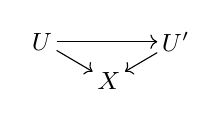
\begin{tikzpicture}[baseline=(current bounding box.center), every node/.style={inner sep=1.5pt, font=\small}]
    \node (U) at (0, 0.5) {$U$};
    \node (Up) at (1.7, 0.5) {$U'$};
    \node (X) at (0.85, 0) {$X$};
    \draw[->] (U) -- (Up);
    \draw[->] (U) -- (X);
    \draw[->] (Up) -- (X);
  \end{tikzpicture}}
\newcommand{\FbFibdiagram}{%
  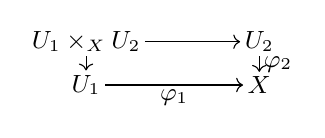
\begin{tikzpicture}[baseline=(current bounding box.center), every node/.style={inner sep=1.5pt, font=\small}]
    \node (A) at (0, 0.55) {$U_1 \times_{X} U_2$};
    \node (U2) at (2.2, 0.55) {$U_2$};
    \node (U1) at (0, 0) {$U_1$};
    \node (X) at (2.2, 0) {$X$};
    \draw[->] (A) -- (U2);
    \draw[->] (A) -- (U1);
    \draw[->] (U2) -- (X) node[midway, right, font=\small] {$\varphi_2$};
    \draw[->] (U1) -- (X) node[midway, below, font=\small] {$\varphi_1$};
  \end{tikzpicture}}
\index{景}
\index{Grothendieck 拓扑}
\index{预层}
\index{层}
\index{平展景}
\index{平坦景}
\index{有限平展拓扑}
\index{完全分解拓扑}
\index{筛}
\index{意象}
\index{连续映射}

为了发展层论以及层的上同调理论(例如在 Grothendieck 1957 年 T\^ohoku 论文中那样)，并不需要有通常意义下的拓扑空间.事实上，只需有一个范畴 $C$ 连同：对 $C$ 的每个对象 $U$，一族特异映射族 $(U_i \to U)_{i \in I}$，称为 $U$ 的覆盖，满足下列公理：
\begin{enumerate}
  \item 对任何覆盖 $(U_i \to U)_{i \in I}$ 和 $C$ 中的任何态射 $V \to U$，纤维积\footnote{对范畴 $C$ 的对象 $X$，$C/X$ 表示对象为 $C$ 中态射 $U \to X$，箭头为交换图
  \begin{center}
  \FbCXdiagram
  \end{center}
  的范畴.使此图交换的态射 $U \to U'$ 也称为 $X$-态射.$C$ 中态射 $\varphi_1 \colon U_1 \to X$，$\varphi_2 \colon U_2 \to X$ 的纤维积 $U_1 \times_{X} U_2$ 是它们在范畴 $C/X$ 中的积.于是，有交换图
  \begin{center}
  \FbFibdiagram
  \end{center}
  具有明显的泛性质.}$U_i \times_{U} V$ 存在，且 $(U_i \times_{U} V \to V)_{i \in I}$ 是 $V$ 的覆盖；
  \item 若 $(U_i \to U)_{i \in I}$ 是 $U$ 的覆盖，且对每个 $i \in I$，$(V_{ij} \to U_i)_{j \in J_i}$ 是 $U_i$ 的覆盖，则族 $(V_{ij} \to U)_{i, j}$ 是 $U$ 的覆盖；
  \item 对 $C$ 中任何 $U$，由单个映射组成的族 $\left(U \xrightarrow{\mathrm{id}} U\right)$ 是 $U$ 的覆盖.
\end{enumerate}
在 (b) 中，映射 $V_{ij} \to U$ 是 $V_{ij} \to U_i \to U$ 的复合.

覆盖系统这时称为 (Grothendieck) 拓扑，而 $C$ 连同该拓扑称为景.若 $T$ 是景，则 $\mathrm{Cat}(T)$ 表示其底层范畴.

例如，设 $X$ 是拓扑空间，$C$ 是对象为 $X$ 的开子集，态射为包含映射的范畴.则族 $(U_i \to U)_{i \in I}$ 且 $(U_i)_{i \in I}$ 是 $U$ 的开覆盖，构成 $C$ 上的 Grothendieck 拓扑.对 $V$ 的开子集 $U$ 与 $U'$，$U \times_{V} U' = U \cap U'$.

景 $T$ 上的集合预层是反变函子 $F \colon \mathrm{Cat}(T) \to \mathbf{Sets}$.于是，对 $\mathrm{Cat}(T)$ 中每个对象 $U$，$F$ 配给一个集合 $F(U)$，对 $\mathrm{Cat}(T)$ 中每个态射 $\varphi \colon U \to V$，配给映射 $F(\varphi) \colon F(V) \to F(U)$，使得 $F(\psi \circ \varphi) = F(\varphi) \circ F(\psi)$ 且 $F(\mathrm{id}_{U}) = \mathrm{id}_{F(U)}$.注意 $T$ 上预层的概念不依赖于覆盖.我们有时把 $F(\varphi) \colon F(V) \to F(U)$ 写为 $a \mapsto a|_{U}$，尽管这可能引起混淆，因为可能有多于一个态射 $U \to V$.

类似地，$T$ 上的(阿贝尔)群或环预层是从 $\mathrm{Cat}(T)$ 到(阿贝尔)群或环范畴的反变函子.

$T$ 上的层是满足层条件的预层 $F$：
\[
(\mathrm{S}) \colon \quad F(U) \to \prod_{i \in I} F(U_i) \rightrightarrows \prod_{(i, j) \in I \times I} F(U_i \times_{U} U_j)
\]
对每个覆盖 $(U_i \to U)$ 正合.于是，$F$ 是层，如果映射
\[
f \mapsto (f|_{U_i}) \colon F(U) \to \prod F(U_i)
\]
把 $F(U)$ 等同于乘积中由这样的族 $(f_i)$ 组成的子集：对所有 $i, j \in I \times I$，
\[
f_i|_{U_i \times_{U} U_j} = f_j|_{U_i \times_{U} U_j}.
\]

当 $T$ 是由拓扑空间产生的景时，这些定义与通常的定义一致.

预层的态射就是函子的态射(又名自然变换)，层的态射是预层的态射.

现在我们列出一些景.本节余下部分中，$X$ 是簇或概形.簇的正则映射族 $(\varphi_i \colon U_i \to U)$ 称为满的，如果 $U = \bigcup \varphi_i(U_i)$，概形的态射族类似.

\textbf{$X$ 上的 Zariski 景} 景 $X_{\mathrm{zar}}$ 是与把 $X$ 看作 Zariski 拓扑的拓扑空间相联系(如上)的景.

\textbf{$X$ 上的平展景} 景 $X_{\mathrm{et}}$ 的底层范畴是 $\mathbf{Et}/X$，其对象是平展态射 $U \to X$，箭头是 $X$-态射 $\varphi \colon U \to V$.覆盖是 $\mathbf{Et}/X$ 中平展态射的满族 $(U_i \to U)$.

\textbf{$X$ 上平展景的变体} 显然，在 Grothendieck 的原始定义中，覆盖取为映射族 $(U_i \to U)_{i \in I}$ 的满族，其中每个映射都是到 $U$ 的某个 Zariski 开子集上的有限平展映射.换言之，定义选取的方式使对该拓扑为``平凡''与 Serre 术语中的``等平凡''一致(见引言).这就是有限平展拓扑，相应的景记为 $X_{\mathrm{fet}}$.\footnote{正确的定义是由 Artin 向他建议的.}

另一个变体由 Nisnevich 提出，它在 $K$ 理论和群概形上同调的研究中被证明有用.它取平展映射的满族 $(U_i \to U)_{i \in I}$ 为覆盖，这些映射有如下性质：对每个 $u \in U$，存在 $i \in I$ 与 $u_i \in U_i$，使得剩余域上的映射 $\kappa(u) \to \kappa(u_i)$ 是同构.该条件对所有 $u \in U$(包括非闭点)都施加，因此即使对代数闭域上的簇，这也不同于平展拓扑.它称为完全分解拓扑，相应的景记为 $X_{\mathrm{cd}}$.$X$ 的点 $x$ 处该拓扑的局部环是 $\mathcal{O}_{X, x}$ 的 Hensel 化(而不是严格 Hensel 化).

在下面两个例子中，我们取 $X$ 为概形.

\textbf{$X$ 上的平坦景} 景 $X_{\mathrm{Fl}}$ 的底层范畴是 $\mathbf{Sch}/X$，即所有 $X$-概形的范畴.覆盖是 $X$-态射的满族 $\left(U_i \xrightarrow{\varphi_i} U\right)$，其中每个 $\varphi_i$ 平坦且有限型.

\textbf{$X$ 上的大平展景} 景 $X_{\mathbf{Et}}$ 的底层范畴是 $\mathbf{Sch}/X$.覆盖是平展 $X$-态射的满族 $(U_i \to U)_{i \in I}$.

\textbf{景 $T_G$} 对每个 pro-有限群 $G$，对应一个景 $T_G$，其底层范畴是 $G$ 的一切有限离散集合的范畴.覆盖是 $G$-映射的任何满族.

\begin{remark}\label{rem:5.1}
(a) 当 $U \to X$ 是 $X$ 的某个覆盖的成员时，我们可以把 $U$ 看作该``拓扑''的 $X$ 的``开子集''.然而注意，对平坦景，$U \to X$ 与 $U' \to X$ 可能都是 $X$ 的``开子集''，但 $X$-态射 $U \to U'$ 可能不把 $U$ 实现为 $U'$ 的``开子集''，即 $U \to X$ 与 $U' \to X$ 可以平坦而 $U \to U'$ 不平坦.

(b) 若底层范畴中的所有概形都拟紧(例如簇)，则可以把覆盖取为有限满族.
\end{remark}

\begin{definition}\label{def:5.2}
设 $T_1$ 与 $T_2$ 是两个景.保持纤维积并把覆盖变为覆盖的函子 $\mathrm{Cat}(T_2) \to \mathrm{Cat}(T_1)$ 称为连续映射 $T_1 \to T_2$.
\end{definition}

例如，拓扑空间的映射 $Y \to X$ 定义相应景的连续映射，当且仅当它按通常意义连续.

有显然的景的连续映射
\[
X_{\mathrm{Fl}} \to X_{\mathbf{Et}} \to X_{\mathrm{et}} \to X_{\mathrm{cd}} \to X_{\mathrm{zar}}.
\]
若 $X = \operatorname{Spec} k$($k$ 是域)，且 $k^{\mathrm{sep}}$ 是 $k$ 的代数闭包，则存在本质互逆的连续映射
\[
T_G \to X_{\mathrm{et}}, \qquad X_{\mathrm{et}} \to T_G,
\]
其中 $G = \operatorname{Gal}(k^{\mathrm{al}}/k)$---见 \S 3.

\begin{remark}\label{rem:5.3}
注意，连续映射 $T_1 \to T_2$ 实际上是反方向的函子.这在 SGA 4 的参与者看来太不合逻辑了，于是他们把连续映射 $T_1 \to T_2$ 定义为保持覆盖的函子 $\mathrm{Cat}(T_1) \to \mathrm{Cat}(T_2)$.然而，这与我们从拓扑空间获得的直觉冲突，在出版版本中被放弃了.
\end{remark}

\textbf{术语对照} 我们称为拓扑的东西在 SGA 4 中称为预拓扑.在那里他们把筛(法语 crible)定义为全子范畴\footnote{这意味着子范畴中的 Hom 集等于所在范畴中的 Hom 集.}，它随任何对象 $V$ 一起包含所有允许到 $V$ 的态射的对象.在 SGA 4 的意义下给范畴 $C$ 一个拓扑，就是给 $C$ 的每个对象 $U$ 一组满足某些自然公理的 $C/U$ 中的筛(同上，II.1).在 SGA 4 中，景被定义为带这种意义的拓扑的范畴.

设 $T$ 是按本节开头定义的景.对任何覆盖 $\mathcal{U} = (U_i \to U)_{i \in I}$，配上筛 $\mathfrak{s}(\mathcal{U})$，其对象是 $\mathrm{Cat}(T)$ 中允许到某个 $U_i$ 的态射的那些对象.由覆盖产生的筛定义了 SGA 4 意义下的拓扑.

意象是等价于景上层范畴的任何范畴.在 SGA 4, p.299 中，论证了意象比景更适合作为研究对象.然而，我在本讲义中不再使用这个词.

有理由更喜欢预拓扑而非拓扑和意象.例如，所有概形范畴上的平展与光滑预拓扑定义相同的层范畴，但给出不同的``局部''概念.见 de Jong 2010 年 6 月 18 日的博客文章.在 Stacks Project 中，他们把景定义为带预拓扑的范畴.

% ============ 6 平展拓扑的层 (原书 pp.42-49) ============
\chapter{平展拓扑的层}\label{sec:6}
\index{Galois 覆盖}
\index{一般 Galois}
\index{层}
\index{常值层}
\index{摩天楼层}
\index{局部常值层}
\index{茎}
\index{忠实平坦}
\index{结构层}

设 $X$ 是簇(或概形).按一般定义，$X_{\mathrm{et}}$ 上的层 $\mathcal{F}$ 是反变函子 $\mathbf{Et}/X \to \mathbf{Sets}$(或 $\mathbf{Ab}$，或 $\ldots$)，使得对每个平展映射 $U \to X$ 与每个平展覆盖 $(U_i \to U)$，
\[
(\mathrm{S}) \colon \quad \mathcal{F}(U) \to \prod_{i \in I} \mathcal{F}(U_i) \rightrightarrows \prod_{(i, j) \in I \times I} \mathcal{F}(U_i \times_{U} U_j)
\]
正合.

注意 $X_{\mathrm{et}}$ 上的层 $\mathcal{F}$ 通过限制对每个平展映射 $U \to X$ 定义了 $U_{\mathrm{zar}}$ 上的层.特别地，若 $U = \coprod U_i$，则 $\mathcal{F}(U) \xrightarrow{\sim} \prod \mathcal{F}(U_i)$.把层条件应用于 $I$ 为空集的情形，发现 $\mathcal{F}(\varnothing)$ 是单元素集合(若 $\mathcal{F}$ 是群层则为零群).这里 $\varnothing$ 是空簇(或空概形).

对 Zariski 覆盖，层条件 (S) 就是熟悉的那个.下面我们考察它对 Galois 覆盖意味着什么.

\subsection*{Galois 覆盖}

设 $\varphi \colon Y \to X$ 是态射，$G$ 是有限群.$G$ 在 $Y$ 上(在 $X$ 上)的右作用是映射 $\alpha \colon G \to \operatorname{Aut}_X(Y)$，使得 $\alpha(gh) = \alpha(h) \circ \alpha(g)$.若 $X$ 与 $Y$ 仿射，使 $\varphi$ 对应于环的映射 $A \to B$，则给出 $G$ 在 $Y$ 上(在 $X$ 上)的右作用与给出 $G$ 在 $A$-代数 $B$ 上的左作用是一回事.

\begin{definition}\label{def:6.1}
设 $Y \to X$ 是忠实平坦映射，$G$ 是作用在 $Y$ 上(在 $X$ 上)的有限群.若态射
\[
Y \times G \to Y \times_{X} Y, \qquad (y, g) \mapsto (y, yg)
\]
是同构，则 $Y \to X$ 称为带群 $G$ 的 $X$ 的 Galois 覆盖.
\end{definition}

这里 $Y \times G$ 表示由 $G$ 的元素指标化的 $Y$ 的副本的不交并：
\[
Y \times G = \coprod_{g} Y_g, \qquad Y_g = Y.
\]
映射 $\mathrm{id} \colon Y_g \to Y$ 与 $g \colon Y_g \to Y$ 定义映射 $Y_g \to Y \times_{X} Y$，而定义中的条件要求这些映射诱导同构 $\coprod_{g} Y_g \to Y \times_{X} Y$.

若 $\varphi \colon Y \to X$ 是 Galois 覆盖，则 $\varphi$ 满，有限且平展，次数等于 $G$ 的阶(因为作平坦基变换后变成这样).反过来，可以证明：若 $Y \to X$ 满，有限且平展，次数等于 $\operatorname{Aut}_X(Y)$ 的阶，则它是带群 $\operatorname{Aut}_X(Y)$ 的 Galois 覆盖.

\begin{remark}\label{rem:6.2}
不可约簇的态射 $\varphi \colon Y \to X$ 称为一般 Galois 的，如果 $k(Y)$ 在 $k(X)$ 上 Galois.有些坏蛋把``一般''去掉，把这样的态射称为 Galois 的.

$A$-代数 $B$ 称为 Galois 的，如果存在作用在 $B$ 上(通过 $A$-代数自同构)的群 $G$，使得 $\operatorname{Spec} B \to \operatorname{Spec} A$ 是带群 $G$ 的 Galois 覆盖.显式地，这意味着 $A \to B$ 忠实平坦，且同态
\[
B \otimes_{A} B \to \prod_{g \in G} B, \qquad b \otimes b' \mapsto (\ldots, b \cdot g(b'), \ldots),
\]
是同构.这里 $\prod_{g \in G} B$ 表示由 $G$ 的元素指标化的 $B$ 的副本的乘积.
\end{remark}

\begin{example}\label{ex:6.3}
设 $K = k[T]/(f(T))$，其中 $k$ 是域，$f(T)$ 是 $k[T]$ 中的首一不可约多项式.若
\[
f(T) = f_1(T)^{e_1} \cdots f_r(T)^{e_r}
\]
是 $f(T)$ 在 $K[T]$ 中分解为互异不可约多项式的幂，则由中国剩余定理，
\[
K \otimes_k K \cong K[T]/(f(T)) \cong \prod K[T]/(f_i(T)^{e_i}).
\]
由此推出，$K$ 是 Galois $k$-代数，当且仅当 $f(T)$ 在 $K[T]$ 中分裂为互异的线性因子，即 $f(T)$ 可分且 $K$ 是它的分裂域.

例如，设 $f(T)$ 是 $n$ 次首一不可约可分多项式.若 $K = k[T]/(f)$ 是 $f$ 的分裂域，则 $K/k$ 是 Galois 的(由标准 Galois 理论)，其 Galois 群 $G$ 是 $f$ 的 $n$ 个根的置换群的 $n$ 阶传递子群.
\end{example}

设 $Y \to X$ 是带群 $G$ 的 Galois 覆盖.则 $G$ 右作用于 $Y$，因此对任意预层 $P$，由于 $P$ 是反变函子，$G$ 左作用于 $P(Y)$.

\begin{proposition}\label{prop:6.4}
设 $Y \to X$ 是带群 $G$ 的 Galois 覆盖，$F$ 是 $X_{\mathrm{et}}$ 上把不交并送到乘积的预层.则 $F$ 对覆盖 $Y \to X$ 满足层条件 (S)，当且仅当限制映射 $F(X) \to F(Y)$ 把 $F(X)$ 等同于 $F(Y)$ 中被 $G$ 固定的元素子集 $F(Y)^{G}$.
\end{proposition}

\begin{proof}
有交换图
\[
\begin{tikzcd}
X \arrow[r, shift left] \arrow[r, shift right] & Y \times_{X} Y \\
X \arrow[u, equal] \arrow[r, shift left] \arrow[r, shift right] & Y \times G \arrow[u, "\sim"']
\end{tikzcd}
\]
其中第一行中的投影映射 $(y, y') \mapsto y$ 与 $(y, y') \mapsto y'$ 分别对应于第二行中的映射 $(y, g) \mapsto y$ 与 $(y, g) \mapsto yg$.把 $F$ 应用于该图，得到交换图
\[
\begin{tikzcd}
F(X) \arrow[r] & F(Y) \arrow[r, shift left] \arrow[r, shift right] & F(Y \times_{X} Y) \\
F(X) \arrow[u, equal] \arrow[r] & F(Y) \arrow[u, "\sim"] \arrow[r, shift left] \arrow[r, shift right] & \prod_{g \in G} F(Y) \arrow[u, "\sim"']
\end{tikzcd}
\]
这里 $\prod_{g \in G} F(Y)$ 是由 $G$ 的元素指标化的 $F(Y)$ 的副本的乘积，而映射 $F(Y) \to \prod_{g \in G} F(Y)$ 分别是
\[
s \mapsto (\ldots, s, \ldots, s, \ldots), \qquad s \mapsto (\ldots, gs, \ldots)
\]
这两个映射在 $s \in F(Y)$ 上一致，当且仅当对所有 $g \in G$，$gs = s$.
\end{proof}

\begin{exercise}\label{exc:6.5}
(a) 设 $F$ 是 $X_{\mathrm{et}}$ 上的 Abel 群层，$Y \to X$ 是带群 $G$ 的 Galois 覆盖.证明复形
\[
F(X) \to F(Y) \to F(Y \times_{X} Y) \to F(Y \times_{X} Y \times_{X} Y) \to \cdots
\]
同构于 $G$ 作用在 $F(Y)$ 上的非齐次上链复形(见 CFT p.62).复形中的每个映射是各投影映射给出的映射的交替和.

(b) 证明 6.3 在把 $k$ 换成局部 Hensel 环时仍然成立.
\end{exercise}

\subsection*{成为层的判别准则}

下一个结果使检验预层是否为层更容易.

\begin{proposition}\label{prop:6.6}
为了验证 $X_{\mathrm{et}}$ 上的预层 $F$ 是层，只需检验 $F$ 对 Zariski 开覆盖和由单个映射组成的平展覆盖 $V \to U$($V$ 与 $U$ 都仿射)满足层条件 (S).
\end{proposition}

\begin{proof}
若 $F$ 对 Zariski 开覆盖满足层条件，则 $F(\coprod U_i) = \prod F(U_i)$.由此推出，对指标集 $I$ 有限的覆盖 $(U_i \to U)_{i \in I}$，序列 (S) 同构于由单个态射 $(\coprod U_i \to U)$ 产生的序列 (S)，因为
\[
\left(\coprod U_i\right) \times_{U} \left(\coprod U_i\right) = \coprod_{(i,j) \in I \times I} \left( U_i \times_{U} U_j \right).
\]
由于仿射簇(或概形)的有限不交并仍是仿射的，命题叙述中的第二个条件蕴含 (S) 对指标集有限且 $U$ 与诸 $U_i$ 仿射的覆盖 $(U_i \to U)_{i \in I}$ 正合.

证明的其余部分只涉及简单的图追图，见 EC II 1.5.
\end{proof}

\begin{remark}\label{rem:6.7}
可以证明，每个有限平展映射 $V \to U$ 都被 Galois 映射 $V' \to U$ 支配，即存在穿过 $V \to U$ 的 Galois 覆盖 $V' \to U$，使得 $V' \to V$ 满射.由此以及命题推出，要验证 $X_{\mathrm{fet}}$(有限平展拓扑---见 \S 5)上的预层 $F$ 是层，只需检验 $F$ 对 Zariski 开覆盖与 Galois 覆盖 $V \to U$ 满足层条件 (S).这些论断对平展拓扑不成立.
\end{remark}

\subsection*{\texorpdfstring{$X_{\mathrm{et}}$ 上层的一些例子}{X\_et 上层的一些例子}}

设 $A \to B$ 是对应于仿射簇(或概形)的满平展态射 $V \to U$ 的环同态.在检验 (\ref{prop:6.6}) 中的第二个条件时，我们通常只用 $A \to B$ 忠实平坦\footnote{回忆平坦同态 $A \to B$ 是忠实平坦的，如果它满足下列等价条件之一：
\begin{enumerate}
  \item 若 $A$-模 $M$ 非零，则 $B \otimes_{A} M$ 非零；
  \item 若 $A$-模的序列 $M' \to M \to M''$ 不正合，则 $B \otimes_{A} M' \to B \otimes_{A} M \to B \otimes_{A} M''$ 也不正合；
  \item 映射 $\operatorname{Spec} B \to \operatorname{Spec} A$ 满射(对仿射 $k$-代数，这等价于 $\operatorname{Specm} B \to \operatorname{Specm} A$ 满射).
\end{enumerate}}这一事实(即不需要用它非分歧).

\textbf{$X_{\mathrm{et}}$ 上的结构层} 对任何平展映射 $U \to X$，定义 $\mathcal{O}_{X_{\mathrm{et}}}(U) = \Gamma(U, \mathcal{O}_U)$.当然，对任何在 $X$ 上平展的 $U$，它在 $U_{\mathrm{zar}}$ 上的限制是层.它是 $X_{\mathrm{et}}$ 上的层这一点由命题~\ref{prop:6.6} 与下一个命题推出.

\begin{proposition}\label{prop:6.8}
对每个忠实平坦同态 $A \to B$，序列
\[
0 \to A \to B \xrightarrow{b \mapsto 1 \otimes b - b \otimes 1} B \otimes_{A} B
\]
正合.
\end{proposition}

\begin{proof}
第 1 步：若 $f \colon A \to B$ 有截面，即满足 $s \circ f = \mathrm{id}$ 的同态 $s \colon B \to A$，则论断成立.

为证明这一点，设 $k \colon B \otimes_{A} B \to B$ 把 $b \otimes b'$ 送到 $b \cdot f(s(b'))$.则
\[
k(1 \otimes b - b \otimes 1) = f(s(b)) - b.
\]
因此，若 $1 \otimes b - b \otimes 1 = 0$，则 $b = f(s(b)) \in f(A)$.

第 2 步：若论断对 $a' \mapsto a' \otimes 1 \colon A' \to A' \otimes_{A} B$ 成立，其中 $A \to A'$ 是某个忠实平坦同态，则它对 $A \to B$ 成立.

$A' \to A' \otimes B$ 的序列由 $A \to B$ 的序列张量 $A'$ 得到.

第 3 步：同态 $b \mapsto b \otimes 1 \colon B \to B \otimes_{A} B$ 有截面，即映射 $b \otimes b' \mapsto bb'$.

由于按假设 $A \to B$ 忠实平坦，这就完成了证明.
\end{proof}

\begin{remark}\label{rem:6.9}
设 $K \to L$ 是按上述意义带群 $G$ 的 Galois 域扩张.则 $L^{G} = K$(由命题~\ref{prop:6.4} 与~\ref{prop:6.8})，从而 $L$ 按通常意义在 $K$ 上 Galois(FT 3.9).
\end{remark}

\textbf{由概形 $Z$ 定义的层} $X$-概形 $Z$ 定义反变函子：
\[
F_Z \colon \mathbf{Et}/X \to \mathbf{Sets}, \qquad F_Z(U) = \operatorname{Hom}_X(U, Z).
\]
我断言这是集合层.容易看出 $F_Z$ 对 Zariski 开覆盖满足层判别准则.因此只需证明，对任何忠实平坦映射 $A \to B$，
\[
Z(A) \to Z(B) \rightrightarrows Z(B \otimes_{A} B)
\]
正合.若 $Z$ 仿射，设由环 $C$ 定义，则序列变为
\[
\operatorname{Hom}_{A\text{-alg}}(C, A) \to \operatorname{Hom}_{A\text{-alg}}(C, B) \rightrightarrows \operatorname{Hom}_{A\text{-alg}}(C, B \otimes_{A} B).
\]
它的正合性立即由命题~\ref{prop:6.8} 推出.非仿射 $Z$ 的情形留给读者.

若 $Z$ 有群结构，则 $F_Z$ 是群层.

\begin{example}\label{ex:6.10}
(a) 设 $\mu_n$ 是由单个方程
\[
T^{n} - 1 = 0
\]
定义的簇(或概形).则 $\mu_n(U)$ 是 $\Gamma(U, \mathcal{O}_U)$ 中 $1$ 的 $n$ 次单位根群.

(b) 设 $\mathbb{G}_{a}$ 是把仿射线看作加法群.则 $\mathbb{G}_{a}(U) = \Gamma(U, \mathcal{O}_U)$(看作 Abel 群).

(c) 设 $\mathbb{G}_{m}$ 是去掉原点的仿射线，看作乘法群.则 $\mathbb{G}_{m}(U) = \Gamma(U, \mathcal{O}_U)^{\times}$.

(d) 设 $\mathrm{GL}_n$ 是在 $n^{2} + 1$ 个变量 $T, T_{11}, \ldots, T_{nn}$ 中由单个方程
\[
T \cdot \det(T_{ij}) = 1
\]
定义的簇(或概形).则 $\mathrm{GL}_n(U) = \mathrm{GL}_n(\Gamma(U, \mathcal{O}_U))$，即元素来自环 $\Gamma(U, \mathcal{O}_U)$ 的可逆 $n \times n$ 矩阵群.例如，$\mathrm{GL}_1 = \mathbb{G}_{m}$.
\end{example}

\textbf{常值层} 设 $X$ 是簇或拟紧概形.对每个集合 $\Lambda$，定义
\[
F_{\Lambda}(U) = \Lambda^{\pi_0(U)}
\]
---由 $U$ 的连通分支集 $\pi_0(U)$ 指标化的 $\Lambda$ 的副本的乘积.配上显然的限制映射，这是层，称为由 $\Lambda$ 定义的 $X_{\mathrm{et}}$ 上的常值层.若 $\Lambda$ 有限，则它是由概形 $X \times \Lambda$($X$ 的由 $\Lambda$ 指标化的副本的不交并)定义的层.当 $\Lambda$ 是群时，$F_{\Lambda}$ 是群层.

\textbf{由凝聚 $\mathcal{O}_X$-模定义的层} 设 $\mathcal{M}$ 是通常代数几何意义下 $X_{\mathrm{zar}}$ 上的凝聚 $\mathcal{O}_X$-模层.对每个平展映射 $\varphi \colon U \to X$，得到 $U_{\mathrm{zar}}$ 上的凝聚 $\mathcal{O}_U$-模层 $\varphi^{*}\mathcal{M}$.例如，若 $U$ 与 $X$ 仿射，分别对应环 $B$ 与 $A$，则 $\mathcal{M}$ 由有限生成 $A$-模 $M$ 定义，$\varphi^{*}\mathcal{M}$ 对应于 $B$-模 $B \otimes_{A} M$.$X_{\mathrm{et}}$ 上有预层 $U \mapsto \Gamma(U, \varphi^{*}\mathcal{M})$，记为 $\mathcal{M}_{\mathrm{et}}$.例如，$(\mathcal{O}_{X_{\mathrm{zar}}})_{\mathrm{et}} = \mathcal{O}_{X_{\mathrm{et}}}$.要验证 $\mathcal{M}_{\mathrm{et}}$ 是层，只需(感谢命题~\ref{prop:6.6})证明：只要 $A \to B$ 忠实平坦，序列
\[
0 \to M \to B \otimes_{A} M \rightrightarrows B \otimes_{A} B \otimes_{A} M
\]
就正合.这可以像 $M = A$ 的情形那样精确证明：再次可以假定 $A \to B$ 有截面，这允许构造收缩同伦.

\begin{example}\label{ex:6.11}
设 $X$ 是域 $k$ 上的簇.对每个态射 $\varphi \colon U \to X$，有正合序列
\[
\varphi^{*}\Omega^{1}_{X/k} \to \Omega^{1}_{U/k} \to \Omega^{1}_{U/X} \to 0
\]
(Hartshorne 1977, II.8.11).若 $\varphi$ 平展，则 $\Omega^{1}_{U/X} = 0$，从而 $\varphi^{*}\Omega^{1}_{X/k} \to \Omega^{1}_{U/k}$ 满射---由于它们是同秩的局部自由层，这蕴含\footnote{提示：利用元素在域中的，列线性无关的方阵可逆.}该映射是同构.因此，$(\Omega^{1}_{X/k})_{\mathrm{et}}$ 在 $U_{\mathrm{zar}}$ 上的限制是 $\Omega^{1}_{U/k}$.
\end{example}

\begin{exercise}\label{exc:6.12}
证明：对每个忠实平坦同态 $A \to B$ 与 $A$-模 $M$，序列
\[
0 \to M \to B \otimes_{A} M \to B \otimes_{A} B \otimes_{A} M \to B \otimes_{A} B \otimes_{A} B \otimes_{A} M \to \cdots
\]
正合.映射 $B^{\otimes i} \otimes_{A} M \to B^{\otimes (i+1)} \otimes_{A} M$ 是 $d_i \otimes 1$，其中 $d_i \colon B^{\otimes i} \to B^{\otimes (i+1)}$ 是在各个位置插入 $1$ 得到的映射的交替和.
\end{exercise}

\textbf{Spec($k$) 上的层} 设 $k$ 是域.$(\operatorname{Spec} k)_{\mathrm{et}}$ 上的 Abel 群预层 $F$ 可以看作共变函子 $\mathbf{Et}/k \to \mathbf{Ab}$(回忆 $\mathbf{Et}/k$ 是平展 $k$-代数的范畴).这样的函子是层，当且仅当对每个有限族 $(A_i)$ 的平展 $k$-代数，$F(\prod A_i) = \bigoplus F(A_i)$，并且对每个域扩张 $K/k_0$($k_0$ 在 $k$ 上有限)的有限 Galois 扩张，$F(k_0) \xrightarrow{\sim} F(K)^{\operatorname{Gal}(K/k_0)}$.

选取 $k$ 的可分闭包 $k^{\mathrm{sep}}$，设 $G = \operatorname{Gal}(k^{\mathrm{sep}}/k)$.对 $(\operatorname{Spec} k)_{\mathrm{et}}$ 上的层 $F$，定义
\[
M_F = \varinjlim F(k'),
\]
其中 $k'$ 遍历 $k^{\mathrm{sep}}$ 中在 $k$ 上有限且 Galois 的子域 $k'$.则 $M_F$ 是离散 $G$-模.

反过来，若 $M$ 是离散 $G$-模，定义
\[
F_M(A) = \operatorname{Hom}_G(F(A), M),
\]
其中 $F(A)$ 是 $G$-集合 $\operatorname{Hom}_{k\text{-alg}}(A, k^{\mathrm{sep}})$(见 \S 3).则 $F_M$ 是 $\operatorname{Spec} k$ 上的层.

函子 $F \mapsto M_F$ 与 $M \mapsto F_M$ 定义了 $(\operatorname{Spec} k)_{\mathrm{et}}$ 上层范畴与离散 $G$-模范畴之间的等价.

\subsection*{茎}

设 $X$ 是代数闭域上的簇，$F$ 是 $X_{\mathrm{et}}$ 上的预层或层.$F$ 在点 $x \in X$ 处的茎是
\[
F_{\bar{x}} = \varinjlim_{(U, u)} F(U),
\]
其中极限遍历 $x$ 的平展邻域.

设 $X$ 是概形，$F$ 是 $X_{\mathrm{et}}$ 上的预层或层.$F$ 在几何点 $\bar{x} \to X$ 处的茎是
\[
F_{\bar{x}} = \varinjlim_{(U, u)} F(U),
\]
其中极限遍历 $\bar{x}$ 的平展邻域.

\begin{example}\label{ex:6.13}
(a) $\mathcal{O}_{X_{\mathrm{et}}}$ 在 $\bar{x}$ 处的茎是 $\mathcal{O}_{X, \bar{x}}$，即 $\bar{x}$ 处的严格局部环.

(b) $F_Z$ 在 $\bar{x}$ 处的茎($Z$ 是 $X$ 上的簇或有限型概形)是 $Z(\mathcal{O}_{X, \bar{x}})$.例如，$\mu_n$,$\mathbb{G}_{a}$，$\mathbb{G}_{m}$ 与 $\mathrm{GL}_n$ 在 $\bar{x}$ 处的茎分别是 $\mu_n(\mathcal{O}_{X, \bar{x}})$,$\mathcal{O}_{X, \bar{x}}$(看作 Abel 群)，$\mathcal{O}^{\times}_{X, \bar{x}}$ 与 $\mathrm{GL}_n(\mathcal{O}_{X, \bar{x}})$.

(c) $\mathcal{M}_{\mathrm{et}}$ 在 $\bar{x}$ 处的茎($\mathcal{M}$ 是凝聚 $\mathcal{O}_X$-模)是 $M_x \otimes_{\mathcal{O}_{X, x}} \mathcal{O}_{X, \bar{x}}$，其中 $M_x$ 是 $\mathcal{M}$ 在 $x$ 处的茎(作为 Zariski 拓扑的层).

(d) 对域 $k$ 上 $\operatorname{Spec} k$ 的层 $F$，在 $\bar{x} = \operatorname{Spec} k^{\mathrm{sep}} \to \operatorname{Spec} k$ 处的茎是 $M_F$(看作 Abel 群).
\end{example}

\subsection*{摩天楼层}

一般地，层 $F$ 称为摩天楼层，如果除有限多个 $x$ 外 $F_{\bar{x}} = 0$.(回忆 $\bar{x}$ 表示 $X$ 的像为 $x \in X$ 的几何点.)我们需要一些特殊的摩天楼层.

设 $X$ 是 Hausdorff 拓扑空间，$x \in X$，$\Lambda$ 是 Abel 群.定义
\[
\Lambda_x(U) = \begin{cases}
\Lambda & \text{若 } x \in U;\\
0 & \text{其他情形}.
\end{cases}
\]
则 $\Lambda_x$ 是 $X$ 上的层.显然，$\Lambda_x$ 在 $y \neq x$ 处的茎是 0，在 $x$ 处的茎是 $\Lambda$.设 $F$ 是 $X$ 上的层.由正向极限的定义，我们看到给出同态 $F_x \overset{\mathrm{def}}{=} \varinjlim_{U} F(U) \to \Lambda$ 与给出相容的映射族 $F(U) \to \Lambda$($U$ 取遍 $x$ 的每个开邻域)是一回事，而给出这样的族与给出层映射 $F \to \Lambda_x$ 是一回事.因此
\[
\operatorname{Hom}(F, \Lambda_x) \cong \operatorname{Hom}(F_x, \Lambda).
\]

现在设 $X$ 是代数闭域上的簇，$x \in X$.对平展映射 $\varphi \colon U \to X$，定义
\[
\Lambda_x(U) = \bigoplus_{u \in \varphi^{-1}(x)} \Lambda.
\]
于是，除非 $x \in \varphi(U)$，$\Lambda_x(U) = 0$，这时它是由映到 $x$ 的 $U$ 的点指标化的 $\Lambda$ 的副本的和.同样，$\Lambda_x$ 是层，它的茎除在 $\bar{x}$ 处为零，在 $\bar{x}$ 处茎为 $\Lambda$.设 $F$ 是 $X$ 上的层，$F_{\bar{x}} \to \Lambda$ 是群同态.选取 $u \in \varphi^{-1}(x)$ 把 $(U, u)$ 实现为 $x$ 的平展邻域，从而确定映射 $F(U) \to F_{\bar{x}} \to \Lambda$.把这些映射对 $u \in \varphi^{-1}(x)$ 组合，得到同态
\[
F(U) \to \Lambda_x(U) \overset{\mathrm{def}}{=} \bigoplus_{u} \Lambda.
\]
它们与限制映射相容，从而定义同态 $F \to \Lambda_x$.这样，我们再次得到同构
\[
\operatorname{Hom}(F, \Lambda_x) \cong \operatorname{Hom}(F_{\bar{x}}, \Lambda).
\]

设 $X$ 是概形，$i \colon \bar{x} \to X$ 是 $X$ 的几何点.对任何平展映射 $\varphi \colon U \to X$，定义
\[
\Lambda_{\bar{x}}(U) = \bigoplus_{\operatorname{Hom}_X(\bar{x}, U)} \Lambda.
\]
同样，这给出 $X_{\mathrm{et}}$ 上的层，并有自然同构 $\operatorname{Hom}(F, \Lambda_{\bar{x}}) \to \operatorname{Hom}(F_{\bar{x}}, \Lambda)$.然而，若 $x \overset{\mathrm{def}}{=} i(\bar{x})$ 不闭，则当 $\bar{y}$ 的像不等于 $x$ 时，$(\Lambda_{\bar{x}})_{\bar{y}} = 0$ 未必成立.因此，除非 $x$ 闭，$\Lambda_{\bar{x}}$ 未必是摩天楼层.

\begin{example}\label{ex:6.14}
设 $X = \operatorname{Spec} k$，几何点 $\bar{x} \to X$ 对应于 $k$ 到其可分闭包 $k^{\mathrm{sep}}$ 的包含.则 $\Lambda_{\bar{x}}$ 是 $X_{\mathrm{et}}$ 上对应于如下离散 $G$-模的层：该模由连续映射 $G \to \Lambda$ 组成(诱导 $G$-模---见 Serre, \emph{Cohomologie Galoisienne}, 2.5).
\end{example}

\subsection*{局部常值层}

设 $X$ 是拓扑空间.$X$ 上的层 $F$ 称为局部常值的，如果对 $X$ 的某个开覆盖中的所有 $U$，$F|_{U}$ 都是常值的.

当 $X$ 连通，局部道路连通且局部单连通时，局部常值层由 $X$ 的基本群分类.

固定点 $x \in X$，设 $F$ 是 $X$ 上的局部常值层.设 $\gamma \colon [0, 1] \to X$ 是满足 $\gamma(0) = x = \gamma(1)$ 的连续映射，即 $\gamma$ 是 $X$ 中基于 $x$ 的闭路.$F$ 在 $[0, 1]$ 上的原像 $\gamma^{*}(F)$ 是常值的.选取 $\gamma^{*}(F)$ 与常值层 $\Lambda$ 的同构，确定了对每个 $0 \leq a \leq 1$ 的同构 $F_{\gamma(a)} \to \Lambda$.由于 $\gamma(0) = \gamma(1) = x$，得到两个同构 $F_x \to \Lambda$，它们相差 $F_x$ 的一个自同构 $\alpha(\gamma)$.映射 $\gamma \mapsto \alpha(\gamma)$ 定义同态 $\pi_1(X, x) \to \operatorname{Aut}(F_x)$.下面是众所周知的：

\begin{proposition}\label{prop:6.15}
映射 $F \mapsto F_x$ 定义了 $X$ 上集合(分别地，Abel 群)的局部常值层范畴与 $\pi_1(X, x)$ 集合(分别地，模)范畴之间的等价.
\end{proposition}

设 $X$ 是代数簇(或概形).$X_{\mathrm{et}}$ 上的层 $F$ 是局部常值的，如果对 $X$ 的某个平展覆盖中的所有 $U \to X$，$F|_{U}$ 都是常值的.

\begin{proposition}\label{prop:6.16}
假定 $X$ 连通，设 $\bar{x}$ 是 $X$ 的几何点.映射 $F \mapsto F_{\bar{x}}$ 定义了 $X$ 上带有限茎的集合(分别地，Abel 群)的局部常值层范畴与有限 $\pi_1(X, \bar{x})$ 集合(分别地，模)范畴之间的等价.
\end{proposition}

\begin{proof}
事实上，可以证明：若 $Z \to X$ 是有限平展映射，则层 $F_Z$ 局部常值且茎有限，而每个这样的层对某个 $Z$ 都是这种形式的；更精确地说，$Z \mapsto F_Z$ 定义了从 $\mathbf{FEt}/X$ 到 $X_{\mathrm{et}}$ 上带有限茎的局部常值层范畴的等价.现在可以应用定理~\ref{thm:3.1} 证明命题.

我概述上述论断的一个证明.考虑满平展态射 $Z \to X$.如上面 6.7 所述，存在满有限平展映射 $Z' \to Z$，使得复合 $Z' \to X$ 是 Galois 覆盖.可以证明 $Z \times_{X} Z'$ 是 $Z'$ 的副本的不交并.层 $F_Z$ 限制为 $Z'$ 上的层 $F_{Z \times_{X} Z'}$，它是常值的.这表明 $F_Z$ 局部常值，并且事实上在有限平展覆盖 $Z' \to Z$ 上变成常值的.

反过来，设 $F$ 是带有限纤维的局部常值层.按假设，存在平展覆盖 $(U_i \to X)_{i \in I}$，使得 $F|_{U_i}$ 常值，从而具有形式 $F_{Z_i}$，其中 $Z_i$ 在 $U_i$ 上有限且平展(事实上，$Z_i$ 是 $U_i$ 的副本的不交并).同构 $(F|_{U_i})|_{U_i \times_{X} U_j} \xrightarrow{\sim} (F|_{U_j})|_{U_i \times_{X} U_j}$ 诱导同构 $Z_i \times_{U_i} (U_i \times_{X} U_j) \to Z_j \times_{U_j} (U_i \times_{X} U_j)$，而下降理论(比较 EC I 2.23)表明由诸 $Z_i$ 与这些同构组成的系统来自某个 $Z \to X$.
\end{proof}

% ============ 7 X_et 上的层范畴 (原书 pp.50-57) ============
\chapter{\texorpdfstring{$X_{\mathrm{et}}$ 上的层范畴}{X\_et 上的层范畴}}\label{sec:7}
\index{Abel 范畴}
\index{预层范畴}
\index{层范畴}
\index{伴随函子}
\index{内射对象}
\index{局部满射}
\index{层化}
\index{Kummer 序列}
\index{Artin-Schreier 序列}
\index{代数空间}
\index{Noether 景}

本节研究 $X_{\mathrm{et}}$ 上 Abel 群层的范畴.特别地，我们证明它是 Abel 范畴.

\subsection*{范畴的一般知识}

设 $T$ 是加性范畴---回忆这意味着集合 $\operatorname{Hom}(A, B)$ 带有 Abel 群结构，使得复合映射双加性，且 $T$ 中每个有限对象族都有直和.$T$ 中的序列
\[
0 \to A \to B \xrightarrow{\alpha} C
\]
正合，如果对所有对象 $T \in T$，
\[
0 \to \operatorname{Hom}(T, A) \to \operatorname{Hom}(T, B) \to \operatorname{Hom}(T, C)
\]
正合，这时 $A$ 称为 $\alpha$ 的核.序列
\[
A \xrightarrow{\beta} B \to C \to 0
\]
正合，如果对所有对象 $T \in T$，
\[
0 \to \operatorname{Hom}(C, T) \to \operatorname{Hom}(B, T) \to \operatorname{Hom}(A, T)
\]
正合，这时 $C$ 称为 $\beta$ 的余核.

设 $T$ 是每个态射都有核与余核的加性范畴.设 $\alpha \colon A \to B$ 是 $T$ 中的态射.$\alpha$ 的余核的核称为 $\alpha$ 的像，$\alpha$ 的核的余核称为 $\alpha$ 的余像.有从 $\alpha$ 的余像到 $\alpha$ 的像的典范态射，若它总是同构，则 $T$ 称为 Abel 范畴.

设 $T$ 是 Abel 范畴.把两个定义结合起来，得到短正合序列
\[
0 \to A \to B \to C \to 0
\]
的概念，从而得到长正合序列的概念.

从一个加性范畴到另一个加性范畴的函子，我们总指加性函子，即要求映射 $\operatorname{Hom}(X, Y) \to \operatorname{Hom}(FX, FY)$ 是 Abel 群同态.

现在设 $C$ 是小范畴\footnote{范畴称为小的，如果它的对象构成集合(而不是类).}，$T$ 是从 $C$ 到 Abel 群范畴 $\mathbf{Ab}$ 的反变函子 $F \colon C \to \mathbf{Ab}$ 的范畴.态射 $\alpha \colon F_1 \to F_2$ 是自然变换.于是，$\alpha$ 给 $C$ 的每个对象 $U$ 配上同态 $\alpha(U) \colon F_1(U) \to F_2(U)$，使得对每个态射 $\varphi \colon V \to U$，图
\[
\begin{tikzcd}[row sep=small, column sep=small]
  F_1(U) \arrow[r, "\alpha(U)"] \arrow[d, "F_1(\varphi)"'] & F_2(U) \arrow[d, "F_2(\varphi)"] \\
  F_1(V) \arrow[r, "\alpha(V)"'] & F_2(V)
\end{tikzcd}
\]
交换.

显然，$T$ 在 $\operatorname{Hom}(F_1, F_2)$ 的显然群结构和直和
\[
(\oplus_i F_i)(U) = \oplus_i F_i(U)
\]
下成为加性范畴.

我们把验证如下论断留作(简单的)习题：

\begin{quote}
\refstepcounter{theorem}\label{item:7.1}
\textbf{7.1} (a) $C$ 上反变函子的序列 $\cdots \to F_i \to G_i \to H_i \to \cdots$ 正合，当且仅当对所有 $U \in C$，序列 $\cdots \to F_i(U) \to G_i(U) \to H_i(U) \to \cdots$ 正合.

(b) $C$ 上反变函子的范畴是 Abel 的.
\end{quote}

\begin{remark}\label{rem:7.2}
在范畴的定义中，要求对每对对象 $X, Y$，$\operatorname{Hom}(X, Y)$ 是集合(而不是类).若 $C$ 不小，则 $C$ 上两个函子之间的自然变换 $\alpha \colon F \to G$ 可能不构成集合.
\end{remark}

\textbf{伴随函子} 设 $C_1$ 与 $C_2$ 是 Abel 范畴.函子 $L \colon C_1 \to C_2$ 与 $R \colon C_2 \to C_1$ 称为伴随的，如果
\[
\operatorname{Hom}_{C_2}(LX_1, X_2) \cong \operatorname{Hom}_{C_1}(X_1, RX_2),
\]
关于 $X_1$ 与 $X_2$ 函子性地成立.也说 $L$ 是 $R$ 的左伴随，$R$ 是 $L$ 的右伴随.若 $L$ 有右伴随，则右伴随唯一(到唯一的同构).

回忆加性范畴的对象 $I$ 称为内射的，如果 $\operatorname{Hom}(\cdot, I)$ 是正合函子.

我们把验证如下论断留作(简单的)习题：

\begin{quote}
\refstepcounter{theorem}\label{item:7.3}
\textbf{7.3} (a) 有左伴随的函子 $R$ 左正合(事实上保持乘积与逆向极限).

(b) 有右伴随的函子 $L$ 右正合(事实上保持直和与正向极限).

(c) 有正合左伴随的函子 $R$ 保持内射对象.
\end{quote}

\subsection*{预层范畴}

设 $X$ 是簇(或概形).按定义，$X_{\mathrm{et}}$ 上 Abel 群的预层就是反变函子 $\mathbf{Et}/X \to \mathbf{Ab}$.为了把上一节的讨论应用于它们，严格地说，我们应该把 $\mathbf{Et}/X$ 换成小范畴.例如，可以把 $\mathbf{Et}/X$ 换成如下形式的平展映射 $U \to X$ 的集合：$U$ 由如下形状的环的商所联系的簇(或概形)拼接而成：$A[T_1, T_2, \ldots]$，其中 $A = \Gamma(V, \mathcal{O}_X)$($V$ 是 $X$ 的某个开仿射子集)，$\{T_1, T_2, \ldots\}$ 是固定符号集.我们将忽略这个问题，并把 $X_{\mathrm{et}}$ 上 Abel 群预层的范畴 $\mathrm{PreSh}(X_{\mathrm{et}})$ 当作 $\mathbf{Et}/X$ 上所有反变函子的范畴来谈论.它是 Abel 范畴，其中 $P' \to P \to P''$ 正合，当且仅当对一切平展映射 $U \to X$，$P'(U) \to P(U) \to P''(U)$ 正合.核，余核，乘积，直和，逆向极限，正向极限等在 $\mathrm{PreSh}(X_{\mathrm{et}})$ 中以显然的方式形成：对每个平展映射 $U \to X$ 构造核，余核等，并取诱导的限制映射.

\subsection*{层范畴}

设 $X$ 是簇(或概形).我们定义范畴 $\mathrm{Sh}(X_{\mathrm{et}})$ 为 $\mathrm{PreSh}(X_{\mathrm{et}})$ 的以 $X_{\mathrm{et}}$ 上 Abel 群层为对象的全子范畴.于是，给出 $X_{\mathrm{et}}$ 上层 $F' \to F$ 的态射就是给出函子的自然变换 $F' \to F$.显然，$\mathrm{Sh}(X_{\mathrm{et}})$ 是加性范畴.我们考察 $\mathrm{Sh}(X_{\mathrm{et}})$ 中的正合性意味着什么.

层(或预层)的态射 $\alpha \colon F \to F'$ 称为局部满的，如果对每个 $U$ 与 $s \in F'(U)$，存在覆盖 $(U_i \to U)$，使得对每个 $i$，$s|_{U_i}$ 在 $F(U_i) \to F'(U_i)$ 的像中.

\begin{lemma}\label{lem:7.4}
设 $\alpha \colon F \to F'$ 是 $X_{\mathrm{et}}$ 上层之间的同态.如下论断等价：
\begin{enumerate}
  \item 层序列 $F \xrightarrow{\alpha} F' \to 0$ 正合；
  \item 映射 $\alpha$ 局部满；
  \item 对每个几何点 $\bar{x} \to X$，映射 $\alpha_{\bar{x}} \colon F_{\bar{x}} \to F'_{\bar{x}}$ 满射.
\end{enumerate}
\end{lemma}

\begin{proof}
(b) $\Rightarrow$ (a).设 $\beta \colon F' \to T$ 是层映射，使得 $\beta \circ \alpha = 0$；我们必须证明这蕴含 $\beta = 0$.

设 $s' \in F'(U)$($U \to X$ 平展).按假设，存在覆盖 $(U_i \to U)_{i \in I}$ 与 $s_i \in F(U_i)$，使得 $\alpha(s_i) = s'|_{U_i}$.现在
\[
\beta(s')|_{U_i} = \beta(s'|_{U_i}) = \beta \circ \alpha(s_i) = 0, \qquad \text{对所有 } i.
\]
由于 $T$ 是层，这蕴含 $\beta(s') = 0$.

(a) $\Rightarrow$ (c).设对某个 $\bar{x} \in X$，$\alpha_{\bar{x}}$ 不满，并设 $\Lambda \neq 0$ 是 $F_{\bar{x}} \to F'_{\bar{x}}$ 的余核.设 $\Lambda_x$ 是上一节定义的层；于是对 $X_{\mathrm{et}}$ 上任意层 $G$，$\operatorname{Hom}(G, \Lambda_x) = \operatorname{Hom}(G_{\bar{x}}, \Lambda)$.映射 $F'_{\bar{x}} \to \Lambda$ 定义非零态射 $F' \to \Lambda_x$，它与 $F \to F'$ 的复合为零(因为它对应于复合 $F_{\bar{x}} \to F'_{\bar{x}} \to \Lambda$).因此，$F \xrightarrow{\alpha} F' \to 0$ 不正合.

(c) $\Rightarrow$ (b).设 $U \to X$ 平展，$\bar{u} \to U$ 是 $U$ 的几何点.复合 $\bar{u} \to U \to X$ 是几何点；记它为 $\bar{x}$.$\bar{u}$ 的平展邻域通过与 $U \to X$ 复合给出 $\bar{x}$ 的平展邻域，而以这种方式产生的 $\bar{x}$ 的平展邻域是共尾的；因此对 $X_{\mathrm{et}}$ 上每个层 $F$，$F_{\bar{u}} \cong F_{\bar{x}}$.

于是，假设蕴含对 $U$ 的每个几何点 $\bar{u} \to U$，$F_{\bar{u}} \to F'_{\bar{u}}$ 满射.设 $s \in F'(U)$.设 $u \in U$，$\bar{u} \to U$ 是像为 $u$ 的 $U$ 的几何点.因为 $F_{\bar{u}} \to F'_{\bar{u}}$ 满射，存在其像包含 $u$ 的平展映射 $V \to U$，使得 $s|_{V}$ 在 $F(V) \to F'(V)$ 的像中.对足够多的 $u \in U$ 应用这个论断，得到所求的覆盖.
\end{proof}

\begin{proposition}\label{prop:7.5}
设
\[
0 \to F' \to F \to F''
\]
是 $X_{\mathrm{et}}$ 上的层序列.如下论断等价：
\begin{enumerate}
  \item 该序列在层范畴中正合；
  \item 对所有平展映射 $U \to X$，序列
  \[
  0 \to F'(U) \to F(U) \to F''(U)
  \]
  正合；
  \item 对 $X$ 的每个几何点 $\bar{x} \to X$，序列
  \[
  0 \to F'_{\bar{x}} \to F_{\bar{x}} \to F''_{\bar{x}}
  \]
  正合.
\end{enumerate}
\end{proposition}

\begin{proof}
在下一小节中，我们证明函子 $i \colon \mathrm{Sh}(X_{\mathrm{et}}) \to \mathrm{PreSh}(X_{\mathrm{et}})$ 有左伴随 $a$.因此(见~\ref{item:7.3})，$i$ 左正合，这证明了 (a) 与 (b) 的等价.

Abel 群正合序列的正向极限正合，从而 (b) 蕴含 (c).逆命题不难，利用 $s \in F(U)$ 为零，当且仅当对 $U$ 的所有几何点 $\bar{u}$, $s_{\bar{u}} = 0$(比较前一个命题 (c) 蕴含 (b) 的证明).
\end{proof}

\begin{proposition}\label{prop:7.6}
设
\[
0 \to F' \to F \to F'' \to 0
\]
是 $X_{\mathrm{et}}$ 上 Abel 群层的序列.如下论断等价：
\begin{enumerate}
  \item 该序列在层范畴中正合；
  \item 映射 $F \to F''$ 局部满，且对所有开平展映射 $U \to X$，序列
  \[
  0 \to F'(U) \to F(U) \to F''(U)
  \]
  正合；
  \item 对每个几何点 $\bar{x} \to X$，序列
  \[
  0 \to F'_{\bar{x}} \to F_{\bar{x}} \to F''_{\bar{x}} \to 0
  \]
  正合.
\end{enumerate}
\end{proposition}

\begin{proof}
结合最后两个命题.
\end{proof}

\begin{remark}\label{rem:7.7}
在最后三个命题的 (c) 中，只需对簇 $X$ 的每个闭点 $x$ 的一个几何点 $\bar{x} \to x \in X$，或对概形 $X$ 的每个点 $x$ 的一个几何点 $\bar{x} \to x \in X$ 检验条件.
\end{remark}

\begin{proposition}\label{prop:7.8}
$X_{\mathrm{et}}$ 上 Abel 群层的范畴 $\mathrm{Sh}(X_{\mathrm{et}})$ 是 Abel 范畴.
\end{proposition}

\begin{proof}
从态射的余像到其像的映射是同构，因为它在茎上同构.
\end{proof}

\begin{example}\label{ex:7.9}
(a) (Kummer 序列).设 $n$ 是不被 $X$ 的任何剩余域的特征整除的整数.例如，若 $X$ 是特征 $p \neq 0$ 的域 $k$ 上的簇，则要求 $p$ 不整除 $n$.考虑序列
\[
0 \to \mu_n \to \mathbb{G}_{m} \xrightarrow{t \mapsto t^{n}} \mathbb{G}_{m} \to 0.
\]
由命题~\ref{prop:7.6} 与例~\ref{ex:6.13}(b)，为证明它正合，只需验证对 $X$ 的每个严格局部环 $A = \mathcal{O}_{X, \bar{x}}$，
\[
0 \to \mu_n(A) \to A^{\times} \xrightarrow{t \mapsto t^{n}} A^{\times} \to 0
\]
正合.除第二个 $A^{\times}$ 处外这都是显然的，而在这里我们必须证明 $A^{\times}$ 的每个元素都是 $n$ 次幂.但 $\frac{d(T^{n} - a)}{dT} = nT^{n-1} \neq 0$(在 $A$ 的剩余域中)，因此 $T^{n} - a$ 在 $A[T]$ 中分裂.

(b) (Artin-Schreier 序列).设 $X$ 是特征 $p \neq 0$ 的域 $k$ 上的簇，考虑序列
\[
0 \to \mathbb{Z}/p\mathbb{Z} \to \mathbb{G}_{a} \xrightarrow{t \mapsto t^{p} - t} \mathbb{G}_{a} \to 0.
\]
同样，为证明该序列正合，必须验证对 $X$ 的每个严格局部环 $A = \mathcal{O}_{X, \bar{x}}$，
\[
0 \to \mathbb{Z}/p\mathbb{Z} \to A \xrightarrow{t \mapsto t^{p} - t} A \to 0
\]
正合.除第二个 $A$ 处外这都是显然的，但 $\frac{d(T^{p} - T - a)}{dT} = -1 \neq 0$(在 $A$ 的剩余域中)，因此 $T^{p} - T - a$ 在 $A[T]$ 中分裂.
\end{example}

\begin{remark}\label{rem:7.10}
若 $p$ 整除 $X$ 的某个剩余域的特征，则
\[
0 \to \mu_p \to \mathbb{G}_{m} \xrightarrow{t \mapsto t^{p}} \mathbb{G}_{m} \to 0
\]
对 $X$ 上的平展拓扑不正合.然而，它对平坦拓扑正合，因为对任何 $a \in \Gamma(U, \mathcal{O}_U)$($U$ 仿射)，方程 $T^{p} - a$ 定义 $U$ 的平坦覆盖.因此 $\mathbb{G}_{m}(U)$ 的每个元素对平坦拓扑局部地都是 $p$ 次幂.
\end{remark}

\subsection*{与预层相伴的层}

本小节中，``层''(或``预层'')指集合的层(或预层).

\begin{definition}\label{def:7.11}
设 $P \to aP$ 是从预层 $P$ 到(某个景上的)层的同态；如果从 $P$ 到层的所有其他同态都唯一穿过 $P \to aP$，即对所有层 $F$，
\[
\operatorname{Hom}(P, F) \cong \operatorname{Hom}(aP, F),
\]
则 $aP$ 称为与 $P$ 相伴的层(或 $P$ 的层化).
\end{definition}

显然，带映射 $P \to aP$ 的 $aP$ 若存在，则唯一到唯一的同构.本小节余下部分中，我们在各种情形中构造 $aP$.首先给出 $F$ 是与 $P$ 相伴的层的判别准则.

设 $P$ 是预层.截面 $s_1, s_2 \in P(U)$ 称为局部相等的，如果对 $U$ 的某个覆盖 $(U_i \to U)_{i \in I}$ 中的所有 $U_i$，$s_1|_{U_i} = s_2|_{U_i}$.层判别准则蕴含层的局部相等截面相等.

\begin{lemma}\label{lem:7.12}
设 $i \colon P \to F$ 是从预层 $P$ 到层 $F$ 的同态.假定：
\begin{enumerate}
  \item $P$ 中在 $F(U)$ 中有相同像的截面只有那些局部相等的截面，且
  \item $i$ 局部满.
\end{enumerate}
则 $(F, i)$ 是与 $P$ 相伴的层.
\end{lemma}

\begin{proof}
设 $i' \colon P \to F'$ 是从 $P$ 到层的第二个映射，对某个 $U$，设 $s \in F(U)$.由 (b)，知道对 $U$ 的某个覆盖 $(U_i \to U)$，存在 $s_i \in P(U_i)$，使得 $i(s_i) = s|_{U_i}$.由 (a)，$i'(s_i) \in F'(U_i)$ 不依赖于 $s_i$ 的选取，而且 $i'(s_i)$ 与 $i'(s_j)$ 在 $F'(U_i \times_{U} U_j)$ 上的限制一致.我们定义 $\alpha(s)$ 为 $F'(U)$ 中限制为所有 $i$ 的 $i'(s_i)$ 的唯一元素.则 $s \mapsto \alpha(s) \colon F \to F'$ 是满足 $i \circ \alpha = i'$ 的唯一同态.
\end{proof}

\begin{lemma}\label{lem:7.13}
设 $P$ 是层 $F$ 的子预层.对每个 $U$，设 $P'(U)$ 是 $F(U)$ 中如下元素的集合：存在覆盖 $(U_i \to U)_{i \in I}$，使得对每个 $i$，$s|_{U_i} \in P(U_i)$(即 $s$ 局部在 $P$ 中).则 $P'$ 是 $F$ 的子层，且 $P \to P'$ 局部满.
\end{lemma}

\begin{proof}
证明是平凡的.
\end{proof}

我们把 $P'$ 称为 $F$ 的由 $P$ 生成的子层.

要构造 $aP$，只需构造满足 (7.12a) 的层 $F$ 与同态 $P \to F$，因为这时 $F$ 的由 $P$ 的像生成的子层就是与 $P$ 相伴的层.

现在我们处理 $X_{\mathrm{et}}$ 上的层.

\begin{lemma}\label{lem:7.14}
若 $i \colon P \to F$ 满足引理~\ref{lem:7.12} 的条件 (a) 和 (b)，则对所有几何点 $\bar{x}$，
\[
i_{\bar{x}} \colon P_{\bar{x}} \to F_{\bar{x}}
\]
是同构.
\end{lemma}

\begin{proof}
这容易由各个定义推出.
\end{proof}

对每个 $x \in X$，选取像为 $x$ 的几何点 $\bar{x} \to X$.对 $X$ 上的预层 $P$，定义 $P^{*} = \prod (P_{\bar{x}})_{\bar{x}}$，其中 $(P_{\bar{x}})_{\bar{x}}$ 是按 \S 6 的方式与 Abel 群 $P_{\bar{x}}$ 相伴的层.则 $P^{*}$ 是层，且自然映射 $P \to P^{*}$ 满足 (\ref{lem:7.12}) 的条件 (a).

\begin{theorem}\label{thm:7.15}
对 $X_{\mathrm{et}}$ 上的每个预层 $P$，存在相伴层 $i \colon P \to aP$.映射 $i$ 在茎上诱导同构 $P_{\bar{x}} \to (aP)_{\bar{x}}$.函子 $a \colon \mathrm{PreSh}(X_{\mathrm{et}}) \to \mathrm{Sh}(X_{\mathrm{et}})$ 正合.
\end{theorem}

\begin{proof}
取 $aP$ 为 $P^{*}$ 的由 $i(P)$ 生成的子层.则 $i \colon P \to aP$ 满足引理~\ref{lem:7.12} 的条件 (a) 和 (b)，前两个论断由它推出.若 $P' \to P \to P''$ 是 Abel 群的正合序列，则对所有 $x \in X$，$P'_{\bar{x}} \to P_{\bar{x}} \to P''_{\bar{x}}$ 正合(因为 Abel 群正合序列的正向极限正合).但最后的序列可以等同于 $(aP')_{\bar{x}} \to (aP)_{\bar{x}} \to (aP'')_{\bar{x}}$，这表明 $aP' \to aP \to aP''$ 正合.
\end{proof}

\begin{example}\label{ex:7.16}
群 $\Lambda$ 定义常值预层 $P_{\Lambda}$，使得对一切 $U \neq \varnothing$，$P_{\Lambda}(U) = \Lambda$.与 $P_{\Lambda}$ 相伴的层是 $F_{\Lambda}$(见 \S 6).

若 $P$ 是 Abel 群层，则 $aP$ 也是.
\end{example}

\begin{remark}\label{rem:7.17}
设 $(F_i)_{i \in I}$ 是 $X_{\mathrm{et}}$ 上 Abel 群层的族.

设 $P$ 是如下预层：对所有平展映射 $U \to X$，$P(U) = \prod_{i \in I} F_i(U)$，限制映射显然.则 $P$ 是层，且它是诸 $F_i$ 的乘积.类似的评注适用于逆向极限与核.

设 $P$ 是如下预层：对所有平展映射 $U \to X$，$P(U) = \bigoplus_{i \in I} F_i(U)$，限制映射显然.一般地，$P$ 不是层，但 $aP$ 是 $\mathrm{Sh}(X_{\mathrm{et}})$ 中诸 $F_i$ 的直和.类似的评注适用于正向极限与余核.

为免读者以为层范畴``就像 Abel 群范畴一样''，让我指出：一般地它没有足够的投射对象；层的正合序列的乘积也不一定正合.
\end{remark}

\begin{aside}\label{asd:7.18}
设 $P$ 是拓扑空间 $X$ 上的集合预层.定义 $E(P)$ 为 $\coprod_{x \in X} P_x$，设 $\pi \colon E(P) \to X$ 是把 $P_x$ 的每个元素送到 $x$ 的映射.$P(U)$ 的 $s$ 定义 $\pi$ 在 $U$ 上的截面 $s \colon U \to E(P)$，即 $x \mapsto s_x$.赋予 $E(P)$ 使所有映射 $s \colon U \to E(P)$ 连续的最细拓扑：于是 $V \subset E(P)$ 开，当且仅当对所有开集 $U \subset X$ 与 $s \in P(U)$，$s^{-1}(V)$ 在 $U$ 中开.

[邀请读者画一幅图：$X$ 表示成水平线，每个茎 $P_x$ 表示成 $x$ 上方的一条短竖线；``层'',``茎'',``截面''这些术语的由来现在应当清楚了.]

对 $X$ 的每个开子集 $U$，设 $F(U)$ 是 $\pi$ 在 $U$ 上的一切连续截面 $s \colon U \to E(P)$ 的集合.显然的映射 $P \to F$ 把 $F$ 实现为与 $P$ 相伴的层.[空间 $E(P)$ 是与 $P$ 相伴的``\'etal\'e 空间''---见 Godement, R., \emph{Th\'eorie des Faisceaux}, Hermann, 1964, II 1.2.可以避免使用这些空间---事实上，Grothendieck 已把它们从数学中驱逐出去了---但它们相当有用，例如用于定义层的逆像.有趣的是，对平展拓扑有一个(需要代数空间的)类比，它例如对定义 Frobenius 映射在上同调群上的作用是有用的.这一方面在讲义的这个版本中强调得不够.
\end{aside}

\begin{aside}\label{asd:7.19}
景 $T$ 上的集合预层 $P$ 称为分离的，如果两个截面只要局部相等就相等.对预层 $P$，定义 $P^{+}$ 为如下预层：
\[
P^{+}(U) = \varinjlim \operatorname{Ker}\left( \prod P(U_i) \rightrightarrows \prod P(U_i \times_{X} U_j) \right),
\]
---极限遍历所有覆盖(假定极限存在).不难证明：
\begin{enumerate}
  \item 若 $P$ 分离，则 $P^{+}$ 是层；
  \item 对任意 $P$，$P^{+}$ 分离.
\end{enumerate}
于是，对每个预层 $P$，$P^{++}$ 是层.事实上，它就是与 $P$ 相伴的层.

正如 Waterhouse 指出的(Pac. J. Math 57 (1975), 597--610)，存在极限不存在的景：问题是极限遍历的是一个类而非集合，不能换成集合上的极限.除了可能 fpqc 景外，这似乎对实际使用的任何景都不是问题.
\end{aside}

\subsection*{Artin 代数空间}

Zariski 拓扑允许我们把仿射簇拼接起来得到一般簇.可以问平展拓扑是否允许我们把仿射簇拼接起来得到更一般的对象.答案是肯定的！

为简单起见，我在固定的代数闭域 $k$ 上工作，只考虑 $k$-簇.

赋予 $\mathbf{Aff}/k$(所有仿射 $k$-簇的范畴)平展拓扑.该景上的层是满足如下条件的反变函子 $A \colon \mathbf{Aff}/k \to \mathbf{Sets}$：对 $\mathbf{Aff}/k$ 中平展映射的每个满族 $(U_i \to U)_{i \in I}$ 满足层条件.注意 $A$ 也可以看作从仿射 $k$-代数到 $\mathbf{Sets}$ 的共变函子.对每个 $k$-簇 $V$，把仿射 $k$-代数 $A$ 送到 $V$ 中坐标在 $A$ 里的点的集合的函子 $A \mapsto V(A)$ 是 $(\mathbf{Aff}/k)_{\mathrm{et}}$ 上的层；此外，由 Yoneda 引理，$k$-簇的范畴可以看作 $(\mathbf{Aff}/k)_{\mathrm{et}}$ 上层范畴的全子范畴.

设 $U$ 是仿射 $k$-簇.$U$ 上的平展等价关系是子簇 $R \subset U \times U$，使得：
\begin{enumerate}
  \item 对每个仿射 $k$-代数 $A$，$R(A)$ 是 $U(A)$ 上的等价关系(按通常意义---这些是集合)；
  \item 包含 $R \hookrightarrow U \times U$ 与投影映射 $U \times U \rightrightarrows U$ 的复合满且平展.
\end{enumerate}
$(\mathbf{Aff}/k)_{\mathrm{et}}$ 上的层 $A$ 是代数空间，如果存在仿射 $k$-簇 $U$，$U$ 上的平展等价关系 $R$ 和把 $A$ 实现为 $U$ 除以 $R$ 的层论商层的层映射 $U \to A$.最后这个条件意味着，
\begin{enumerate}
  \item 对每个仿射 $k$-代数 $A$ 与 $s_1, s_2 \in U(A)$，$s_1$ 与 $s_2$ 在 $A(A)$ 中有相同的像，当且仅当 $(s_1, s_2) \in R(A)$；
  \item 层映射 $U \to A$ 局部满.
\end{enumerate}
代数簇的范畴是代数空间范畴的全子范畴.代数空间比代数簇有许多优点，我只提两个.

代数空间在群作用下的商更可能存在.例如，Hironaka 构造了非奇异 3 维簇 $V$ 和 2 阶群 $G$ 在 $V$ 上的自由作用，使得商 $V/G$ 不作为代数簇存在(问题是存在不包含在任何仿射开集中的 $G$ 轨道).有限群自由作用下的代数空间的商总是作为代数空间存在(Artin 1973, p.109).关于代数空间商的非常一般的定理，见 Keel, S., and Mori, S., \emph{Quotients by groupoids}, Annals of Mathematics, 145 (1997), 193--213.

从 $\mathbb{C}$ 上完备代数簇的范畴到紧解析空间范畴有自然的全忠实函子 $V \mapsto V(\mathbb{C})$，但对这个函子的本质像没有方便的刻画.对完备代数空间范畴有：它由这样的紧解析空间 $M$ 组成：$M$ 上亚纯函数域有等于 $M$ 的维数的超越次数(这些是 Moishezon 空间).

\subsection*{附记}

设 $X$ 是簇(或拟紧概形).则 $X$ 的每个开子集 $U$ 都拟紧，即 $U$ 的开子集覆盖 $U = \bigcup U_i$ 都有有限子覆盖.此外，由于我把平展态射定义为有限型(而不是局部有限型)，每个在 $X$ 上平展的 $U$ 都拟紧.因为平展态射是开的，这蕴含每个平展覆盖 $(U_i \to U)_{i \in I}$ 都有有限子覆盖.每个覆盖族都含有限覆盖子族的景称为 Noether 景.注意拓扑空间 $X$ 定义的景很少是 Noether 的：若 $X$ 是 Hausdorff 的，它的景是 Noether 的，当且仅当 $X$ 的每个开子集都紧.

\begin{quote}
\refstepcounter{theorem}\label{item:7.20}
\textbf{7.20} 对 Noether 景，要证明预层是层，只需对有限覆盖检验层条件.由此推出，按朴素(即预层)方式形成的层的直和与正向极限仍是层，并且由此推出上同调与直和及(对有向集的)正向极限交换.见 EC III.3.
\end{quote}

% ============ 8 层的直像与逆像 (原书 pp.58-63) ============
\chapter{层的直像与逆像}\label{sec:8}
\index{直像}
\index{逆像}
\index{零延拓}
\index{内射对象}
\index{支集}
\index{紧支集}

\subsection*{层的直像}

设 $\varphi \colon Y \to X$ 是簇(或概形)的态射，$P$ 是 $Y_{\mathrm{et}}$ 上的预层.对平展映射 $U \to X$，定义
\[
\varphi_{*}P(U) = P(U \times_{X} Y).
\]
由于 $U \times_{X} Y \to Y$ 平展(见命题~\ref{prop:2.11})，这个定义有意义.配上显然的限制映射，$\varphi_{*}P$ 成为 $X_{\mathrm{et}}$ 上的预层.

\begin{lemma}\label{lem:8.1}
若 $F$ 是层，则 $\varphi_{*}F$ 也是层.
\end{lemma}

\begin{proof}
对 $X$ 上的簇(或概形) $V$，设 $V_Y$ 表示 $Y$ 上的簇(或概形) $V \times_{X} Y$.则 $V \mapsto V_Y$ 是把平展映射送到平展映射，把满映射族送到满映射族，把 $X$ 上的纤维积送到 $Y$ 上的纤维积的函子.

设 $(U_i \to U)$ 是 $\mathbf{Et}/X$ 中平展映射的满族.则 $(U_{iY} \to U_Y)$ 是 $\mathbf{Et}/Y$ 中平展映射的满族，从而
\[
F(U_Y) \to \prod F(U_{iY}) \rightrightarrows \prod F(U_{iY} \times_{Y} U_{jY})
\]
正合.但这等于序列
\[
(\varphi_{*}F)(U) \to \prod (\varphi_{*}F)(U_i) \rightrightarrows \prod (\varphi_{*}F)(U_i \times_{X} U_j),
\]
因此它也正合.
\end{proof}

显然，函子
\[
\varphi_{*} \colon \mathrm{PreSh}(Y_{\mathrm{et}}) \to \mathrm{PreSh}(X_{\mathrm{et}})
\]
正合.因此，它的限制
\[
\varphi_{*} \colon \mathrm{Sh}(Y_{\mathrm{et}}) \to \mathrm{Sh}(X_{\mathrm{et}})
\]
左正合.它通常不右正合：$F \to F'$ 局部满不蕴含 $\varphi_{*}F \to \varphi_{*}F'$ 局部满.例如，若 $X$ 是代数闭域上的代数簇，$\varphi \colon X \to P$ 是把 $X$ 映到点的映射，则 $\varphi_{*}$ 本质上就是把层 $F$ 送到其整体截面群 $\Gamma(X, F)$ 的函子，而 $F \to F'$ 局部满不蕴含 $\Gamma(X, F) \to \Gamma(X, F')$ 满射.

\begin{example}\label{ex:8.2}
设 $i \colon \bar{x} \to X$ 是 $X$ 的几何点.函子 $F \mapsto F(\bar{x})$ 把 $\bar{x}$ 上的层范畴等同于 Abel 群范畴.设 $\Lambda$ 是看作 $\bar{x}$ 上层的 Abel 群.则 $i_{*}\Lambda = \Lambda_{\bar{x}}$，即 \S 6 中定义的摩天楼层.

$Y$ 的几何点 $\bar{y} \to Y$ 通过 $\bar{y} \to Y \xrightarrow{\varphi} X$ 定义 $X$ 的几何点，记为 $\bar{x}$(或 $\varphi(\bar{y})$).显然
\[
(\varphi_{*}F)_{\bar{x}} = \varinjlim F(V),
\]
其中极限遍历 $\bar{y}$ 的所有这样的平展邻域：对 $\bar{x}$ 的某个平展邻域 $U$，它们具有形式 $U_Y$.于是，有典范映射
\[
(\varphi_{*}F)_{\bar{x}} \to F_{\bar{y}}.
\]
一般地，这个映射既不是单射也不是满射.
\end{example}

\begin{proposition}\label{prop:8.3}
(a) 设 $\varphi \colon V \hookrightarrow X$ 是开浸入，即开子簇(或子概形)到 $X$ 的包含.则
\[
(\varphi_{*}F)_{\bar{x}} = \begin{cases}
F_{\bar{x}} & x \in V;\\
? & x \notin V.
\end{cases}
\]
(b) 设 $\varphi \colon Z \hookrightarrow X$ 是闭浸入，即闭子簇(或子概形)到 $X$ 的包含.则
\[
(\varphi_{*}F)_{\bar{x}} = \begin{cases}
F_{\bar{x}} & x \in Z;\\
0 & x \notin Z.
\end{cases}
\]
(c) 设 $\varphi \colon Y \to X$ 是有限映射.则
\[
(\varphi_{*}F)_{\bar{x}} = \bigoplus_{y \mapsto x} F^{d(y)}_{\bar{y}},
\]
其中 $d(y)$ 是 $\kappa(y)$ 在 $\kappa(x)$ 上的可分次数.例如，若 $\varphi$ 是代数闭域上次数为 $d$ 的簇的有限平展映射，则
\[
(\varphi_{*}F)_{\bar{x}} = F^{d}_{\bar{x}}.
\]
\end{proposition}

\begin{proof}
当 $\varphi \colon V \hookrightarrow X$ 是浸入(开的或闭的)时，对任何态射 $\varphi' \colon U \to X$，纤维积 $U \times_{X} V = \varphi'^{-1}(V)$.

(a) 若 $x \in V$，则对 $\bar{x}$ 的任何``足够小''的平展邻域 $\varphi' \colon U \to X$, $\varphi'(U) \subset V$，从而 $U = \varphi'^{-1}(V) = U \times_{X} V$.因此，$\bar{x}$ 的具有形式 $U_V$ 的平展邻域构成共尾集，这证明了第一个等式.关于第二个，除了指出当 $x \notin V$ 时 $(\varphi_{*}F)_{\bar{x}}$ 不必为零(见下面的例子)外，没什么可说的.

(b) 若 $x \notin Z$，则对 $\bar{x}$ 的任何``足够小''的平展邻域 $\varphi' \colon U \to X$, $\varphi'(U) \cap Z = \varnothing$，从而 $U \times_{X} Z = \varphi'^{-1}(Z) = \varnothing$；因此 $F(U_Z) = 0$.当 $x \in Z$ 时，必须看到每个平展映射 $\bar{\varphi}' \colon \bar{U} \to Z$($x \in \varphi'(\bar{U})$)都``延拓''为平展映射 $\varphi' \colon U \to X$.用环的语言，这相当于证明平展同态 $\bar{A} \to \bar{B}$($\bar{A} = A/\mathfrak{a}$)提升为平展同态 $A \to B$.但这很容易：我们可以假定 $\bar{B} = (\bar{A}[T]/(\bar{f}(T)))_{\bar{b}}$，其中 $\bar{f}(T)$ 是首一多项式，使得 $\bar{f}'(T)$ 在 $(\bar{A}[T]/(\bar{f}(T)))_{\bar{b}}$ 中可逆---见 \S 2(标准平展态射)；选取提升 $\bar{f}(T)$ 的 $f(T) \in A[T]$，对适当的 $b$ 置 $B = (A[T]/(f(T)))_b$.

(c) 我们省略证明.
\end{proof}

\begin{corollary}\label{cor:8.4}
若 $\varphi$ 有限或是闭浸入，则函子 $\varphi_{*}$ 正合.
\end{corollary}

\begin{proof}
这由该命题与命题~\ref{prop:7.6} 推出.
\end{proof}

\begin{example}\label{ex:8.5}
我们列出一些例子，都是类比.

(a) 设 $X$ 是以原点为中心的 $\mathbb{R}^{2}$ 中半径 1 的开圆盘，$U = X \setminus \{(0,0)\}$，$j$ 是包含 $U \hookrightarrow X$.设 $F$ 是对应于 $\pi_1(U, u)$-模 $F$ 的 $U$ 上的局部常值层---回忆 $\pi_1(U, u) = \mathbb{Z}$(见命题~\ref{prop:6.15}；这里 $u$ 是 $U$ 的任意点).则
\[
(j_{*}F)_{(0,0)} = F^{\pi_1(U,u)} \quad (\text{被 } \pi_1 \text{ 固定的元素}).
\]

(b) 设 $X$ 是代数闭域上的仿射线，$U = X \setminus \{0\}$，$j$ 是包含 $U \hookrightarrow X$.设 $F$ 是对应于 $\pi_1(U, \bar{u})$-模 $F$ 的 $U$ 上的局部常值层---回忆 $\pi_1(U, \bar{u}) = \widehat{\mathbb{Z}}$.则
\[
(j_{*}F)_{\bar{0}} = F^{\pi_1(U,\bar{u})} \quad (\text{被 } \pi_1 \text{ 固定的元素}).
\]

(c) 设 $X = \operatorname{Spec} R$，其中 $R$ 是 Hensel 离散赋值环，$U = \operatorname{Spec} K$，其中 $K$ 是 $R$ 的分式域，$j$ 是包含 $U \hookrightarrow X$.设 $F$ 是对应于 $\pi_1(U, \bar{u})$-模 $F$ 的 $U$ 上的局部常值层---回忆 $\pi_1(U, \bar{u}) = \operatorname{Gal}(K^{\mathrm{sep}}/K)$.这里 $\bar{u}$ 是对应于包含 $K \hookrightarrow K^{\mathrm{sep}}$ 的几何点.设 $I$(惯性群)是 $\pi_1(U, \bar{u})$ 中平凡作用于剩余域的元素组成的子群.则
\[
(j_{*}F)_{\bar{x}} = F^{I} \quad (\text{被 } I \text{ 固定的元素}),
\]
其中 $x$ 是 $\operatorname{Spec} R$ 的闭点.
\end{example}

\begin{proposition}\label{prop:8.6}
对任意态射 $Z \xrightarrow{\varphi} Y \xrightarrow{\varphi'} X$，$(\varphi' \circ \varphi)_{*} = \varphi'_{*} \circ \varphi_{*}$.
\end{proposition}

\begin{proof}
这由定义显然.
\end{proof}

\subsection*{层的逆像}

设 $\varphi \colon Y \to X$ 是簇(或概形)的态射.我们将定义函子 $\varphi_{*}$ 的左伴随.设 $P$ 是 $X_{\mathrm{et}}$ 上的预层.对平展映射 $V \to Y$，定义
\[
P'(V) = \varinjlim P(U),
\]
其中正向极限遍历交换图
\[
\begin{tikzcd}[row sep=small, column sep=small]
  V \arrow[r] \arrow[rd] & U \arrow[d] \\
                         & X
\end{tikzcd}
\]
$U \to X$ 平展，且映射 $V \to U$ 与 $V \to Y$ 使图交换.容易看出，对 $Y$ 上的任意预层 $Q$，下列对象之间有自然的双射对应：
\begin{itemize}
  \item 态射 $P' \to Q$；
  \item 由如上交换图指标化的映射族 $P(U) \to Q(V)$，与限制映射相容；
  \item 态射 $P \to \varphi_{*}Q$.
\end{itemize}
因此
\[
\operatorname{Hom}_{Y_{\mathrm{et}}}(P', Q) \cong \operatorname{Hom}_{X_{\mathrm{et}}}(P, \varphi_{*}Q),
\]
关于 $P$ 与 $Q$ 函子性地成立.遗憾的是，即使 $P$ 是层，$P'$ 也不必是层.因此，对 $X_{\mathrm{et}}$ 上的层 $F$，定义 $\varphi^{*}F = a(F')$.则对 $Y_{\mathrm{et}}$ 上的任意层 $G$，
\[
\operatorname{Hom}_{Y_{\mathrm{et}}}(\varphi^{*}F, G) \cong \operatorname{Hom}_{Y_{\mathrm{et}}}(F', G) \cong \operatorname{Hom}_{X_{\mathrm{et}}}(F, \varphi_{*}G),
\]
从而 $\varphi^{*}$ 是 $\varphi_{*} \colon \mathrm{Sh}(Y_{\mathrm{et}}) \to \mathrm{Sh}(X_{\mathrm{et}})$ 的左伴随.

\begin{proposition}\label{prop:8.7}
对任意态射 $Z \xrightarrow{\varphi} Y \xrightarrow{\varphi'} X$，$(\varphi' \circ \varphi)^{*} = \varphi^{*} \circ \varphi'^{*}$.
\end{proposition}

\begin{proof}
两者都是 $(\varphi' \circ \varphi)_{*} = \varphi'_{*} \circ \varphi_{*}$ 的左伴随.
\end{proof}

\begin{example}\label{ex:8.8}
设 $\varphi \colon U \to X$ 是平展态射.对 $X_{\mathrm{et}}$ 上的任意层 $F$ 与 $U_{\mathrm{et}}$ 上的任意层 $G$，容易看出
\[
\operatorname{Hom}(F|_{U_{\mathrm{et}}}, G) \cong \operatorname{Hom}(F, \varphi_{*}G)
\]
---在两种情形中，给出态射都是给出由平展映射 $V \to U$ 指标化的，与限制相容的映射族 $F(V) \to G(V)$.因此，在这种情况下，$\varphi^{*} \colon \mathrm{Sh}(X_{\mathrm{et}}) \to \mathrm{Sh}(U_{\mathrm{et}})$ 就是限制映射.

这也可以直接从 $\varphi^{*}$ 的定义看出，因为对每个 $V \to U$，取极限的图族中有终对象，即
\[
\begin{tikzcd}[row sep=small, column sep=small]
  V \arrow[r, equal] \arrow[rd] & V \arrow[d] \\
  U \arrow[r, "\varphi"] & X
\end{tikzcd}
\]
\end{example}

\begin{remark}\label{rem:8.9}
设 $i \colon \bar{x} \to X$ 是 $X$ 的几何点.对 $X_{\mathrm{et}}$ 上的任意层 $F$，$(i^{*}F)(\bar{x}) = F_{\bar{x}}$---这由 $i^{*}$ 与 $F_{\bar{x}}$ 的定义显然.因此，对任意态射 $\varphi \colon Y \to X$ 与 $Y$ 的几何点 $i \colon \bar{y} \to Y$，
\[
(\varphi^{*}F)_{\bar{y}} = i^{*}(\varphi^{*}F)(\bar{y}) = F_{\bar{x}},
\]
其中 $\bar{x}$ 是 $X$ 的几何点 $\bar{y} \xrightarrow{i} Y \xrightarrow{\varphi} X$.

由于这对 $Y$ 的所有几何点都成立，我们看到 $\varphi^{*}$ 正合，从而 $\varphi_{*}$ 保持内射对象(由 7.3).
\end{remark}

\begin{remark}\label{rem:8.10}
设 $F_Z$ 是由簇 $Z$ 定义的 $X_{\mathrm{et}}$ 上的层.则 $\varphi^{*}(F_Z)$ 是由簇 $Z \times_{Y} X$ 定义的层 $F_{Z \times_{Y} X}$ 这一点不总为真.例如，若 $\varphi \colon X \to P$ 是代数闭域 $k$ 上的簇到点的映射，则 $\varphi^{*}(\mathbb{G}_{a})$ 是由群 $\mathbb{G}_{a}(k) = k$ 定义的常值层.

然而，当 $\varphi$ 平展或 $Z \to X$ 平展时，$\varphi^{*}(F_Z) = F_{Z \times_{Y} X}$ 为真.
\end{remark}

\begin{remark}\label{rem:8.11}
对拓扑空间的连续映射 $\varphi \colon Y \to X$，可以用相伴的 \'etal\'e 空间非常简单地描述层的逆像：$\varphi^{*}(F)$ 是如下层：它在开子集 $U \subset Y$ 上的截面是连续映射 $s \colon U \to E(F)$，使得对所有 $u$，$s(u)$ 位于 $\varphi(u)$ 上的茎中.
\end{remark}

\subsection*{足够内射对象的存在性}

设 $X$ 是簇(或概形).

\begin{proposition}\label{prop:8.12}
$\mathrm{Sh}(X_{\mathrm{et}})$ 中的每个层 $F$ 都能嵌入内射层.
\end{proposition}

\begin{proof}
对每个 $x \in X$，选取像为 $x$ 的几何点 $i_x \colon \bar{x} \to X$，并把 Abel 群 $F_{\bar{x}}$ 嵌入内射 Abel 群 $I(x)$.则 $I_x \overset{\mathrm{def}}{=} i_{x*}(I(x))$ 内射(见注记~\ref{rem:8.9}).由于内射对象的乘积内射，$I \overset{\mathrm{def}}{=} \prod I_x$ 是内射层.复合 $F \hookrightarrow P^{*} \hookrightarrow I$ 就是所求的嵌入.
\end{proof}

\subsection*{零延拓}

设 $X$ 是簇(或概形)，$j \colon U \hookrightarrow X$ 是开浸入.如我们上面所述，对 $U_{\mathrm{et}}$ 上的层 $F$，$j_{*}F$ 在 $U$ 之外的点处的茎不必为零.现在我们定义``零延拓''函子 $j_{!}$，使得 $j_{!}F$ 确实有这个性质.

设 $P$ 是 $U_{\mathrm{et}}$ 上的预层.对任何平展映射 $\varphi' \colon V \to X$，定义
\[
P_{!}(V) = \begin{cases}
P(V) & \text{若 } \varphi'(V) \subset U;\\
0 & \text{其他情形}.
\end{cases}
\]
则 $P_{!}$ 是 $X_{\mathrm{et}}$ 上的预层，且对 $X_{\mathrm{et}}$ 上的任何其他预层 $Q$，态射 $P \to Q|_{U}$ 唯一延拓为态射 $P_{!} \to Q$(显然).因此
\[
\operatorname{Hom}_{X_{\mathrm{et}}}(P_{!}, Q) \cong \operatorname{Hom}_{U_{\mathrm{et}}}(P, Q|_{U})
\]
函子性地成立.遗憾的是，即使 $P$ 是层，$P_{!}$ 也不必是层.因此，对 $U_{\mathrm{et}}$ 上的层 $F$，定义 $j_{!}F = a(F_{!})$.则对 $X_{\mathrm{et}}$ 上的任意层 $G$，
\[
\operatorname{Hom}_{X_{\mathrm{et}}}(j_{!}F, G) \cong \operatorname{Hom}_{X_{\mathrm{et}}}(F_{!}, G) \cong \operatorname{Hom}_{U_{\mathrm{et}}}(F, G|_{U}),
\]
从而 $j_{!}$ 是 $j^{*} \colon \mathrm{Sh}(X_{\mathrm{et}}) \to \mathrm{Sh}(U_{\mathrm{et}})$ 的左伴随.

\begin{proposition}\label{prop:8.13}
设 $j \colon U \hookrightarrow X$ 是开浸入.对 $U_{\mathrm{et}}$ 上的任意层 $F$ 与几何点 $\bar{x} \to X$,
\[
(j_{!}F)_{\bar{x}} = \begin{cases}
F_{\bar{x}} & x \in U;\\
0 & x \notin U.
\end{cases}
\]
\end{proposition}

\begin{proof}
由引理~\ref{lem:7.14}，只需对把 $j_{!}F$ 换成 $F_{!}$ 证明，这时它立即由定义推出.
\end{proof}

\begin{corollary}\label{cor:8.14}
函子 $j_{!} \colon \mathrm{Sh}(U_{\mathrm{et}}) \to \mathrm{Sh}(X_{\mathrm{et}})$ 正合，且 $j^{*}$ 保持内射对象.
\end{corollary}

\begin{proof}
论断的第一部分由该命题与命题~\ref{prop:7.6} 推出，第二部分由第一部分与~\ref{item:7.3} 推出.
\end{proof}

设 $Z$ 是 $U$ 在 $X$ 中的补集，用 $i$ 表示包含 $Z \hookrightarrow X$.设 $F$ 是 $X_{\mathrm{et}}$ 上的层.有典范态射 $j_{!}j^{*}F \to F$(由伴随性对应于 $j^{*}F$ 上的恒等映射)与典范态射 $F \to i_{*}i^{*}F$(由伴随性对应于 $i^{*}F$ 上的恒等映射).

\begin{proposition}\label{prop:8.15}
对 $X$ 上的任意层 $F$，序列
\[
0 \to j_{!}j^{*}F \to F \to i_{*}i^{*}F \to 0
\]
正合.
\end{proposition}

\begin{proof}
这可以在茎上检验.对 $x \in U$，茎序列是
\[
0 \to F_{\bar{x}} \xrightarrow{\mathrm{id}} F_{\bar{x}} \to 0 \to 0;
\]
对 $x \notin U$，茎序列是
\[
0 \to 0 \to F_{\bar{x}} \xrightarrow{\mathrm{id}} F_{\bar{x}} \to 0.
\]
两者显然正合.
\end{proof}

\begin{remark}\label{rem:8.16}
可以对任何平展映射 $j \colon U \to X$ 定义 $j_{!}$.设 $F$ 是 $U_{\mathrm{et}}$ 上的层.对任何平展映射 $\varphi' \colon V \to X$，定义
\[
F_{!}(V) = \bigoplus_{\alpha} F(V),
\]
其中求和遍历满足 $j \circ \alpha = \varphi'$ 的态射 $\alpha \colon V \to U$.则 $F_{!}$ 是 $X_{\mathrm{et}}$ 上的预层，我们定义 $j_{!}F$ 为它的相伴层.同样，$j_{!}$ 是 $j^{*}$ 的左伴随且正合.因此 $j^{*}$ 保持内射对象.
\end{remark}

\subsection*{\texorpdfstring{$X = U \cup Z$ 上的层}{X = U ∪ Z 上的层}}

设 $X$ 是簇(或概形)，
\[
U \xrightarrow{j} X \xleftarrow{i} Z
\]
是态射，其中 $j$ 是开浸入，$i$ 是闭浸入，且 $X = j(U) \cup i(Z)$.我们把 $U$ 与 $Z$ 等同于 $X$ 的子簇(或子概形).

由 $X_{\mathrm{et}}$ 上的层 $F$，得到 $Z$ 上的层 $F_1 \overset{\mathrm{def}}{=} i^{*}F$ 与 $U$ 上的层 $F_2 = j^{*}F$.此外，有典范同态 $F \to j_{*}j^{*}F$(由伴随性对应于 $j^{*}F$ 上的恒等映射).对它应用 $i^{*}$，得到态射 $\Phi_F \colon F_1 \to i^{*}j_{*}F_2$.

设 $\mathrm{Tr}(X, U, Z)$ 是如下范畴：对象是三元组 $(F_1, F_2, \Phi)$，其中 $F_1$ 是 $Z_{\mathrm{et}}$ 上的层，$F_2$ 是 $U_{\mathrm{et}}$ 上的层，$\Phi$ 是映射 $F_1 \to i^{*}j_{*}F_2$.态射 $(F_1, F_2, \Phi) \to (F'_1, F'_2, \Phi')$ 是满足下图交换的态射对 $\psi_1 \colon F_1 \to F'_1$ 与 $\psi_2 \colon F_2 \to F'_2$:
\[
\begin{tikzcd}
F_1 \arrow[r, "\Phi"] \arrow[d, "\psi_1"] & i^{*}j_{*}F_2 \arrow[d, "i^{*}j_{*}\psi_2"] \\
F'_1 \arrow[r, "\Phi'"'] & i^{*}j_{*}F'_2
\end{tikzcd}
\]

\begin{proposition}\label{prop:8.17}
函子 $F \mapsto (F_1, F_2, \Phi_F)$ 是等价 $\mathrm{Sh}(X_{\mathrm{et}}) \to \mathrm{Tr}(X, U, Z)$.
\end{proposition}

\begin{proof}
本质逆由函子
\[
(F_1, F_2, \Phi) \mapsto i_{*}F_1 \times_{i_{*}i^{*}j_{*}F_2} j_{*}F_2
\]
给出.细节见 EC p.74.
\end{proof}

在这个范畴等价下，
\[
0 \to j_{!}j^{*}F \to F \to i_{*}i^{*}F \to 0
\]
对应于正合序列
\[
0 \to (0, j^{*}F, 0) \to (i^{*}F, j^{*}F, \Phi_F) \to (i^{*}F, 0, 0) \to 0.
\]
当且仅当 $\Phi_F = 0$ 时该序列分裂.

设 $Y$ 是 $X$ 的子集.我们说层 $F$ 的支集在 $Y$ 中，如果只要 $x \notin Y$ 就有 $F_{\bar{x}} = 0$.

\begin{corollary}\label{cor:8.18}
对任何闭浸入 $i \colon Z \hookrightarrow X$，$i_{*}$ 定义了 $Z_{\mathrm{et}}$ 上层范畴与支集在 $Z$ 中的 $X_{\mathrm{et}}$ 上层范畴之间的等价.
\end{corollary}

\begin{proof}
这由该命题与显然的事实推出：$F$ 的支集在 $Z$ 中，当且仅当它对应于形如 $(F_1, 0, 0)$ 的三元组.
\end{proof}

% ============ 9 上同调: 定义与基本性质 (原书 pp.64-69) ============
\chapter{上同调：定义与基本性质}\label{sec:9}
\index{上同调}
\index{导出函子}
\index{Ext 群}
\index{带支集上同调}
\index{切除}
\index{同伦公理}
\index{有理等价}
\index{维数公理}

在上一节中，我们证明了 Abel 群层范畴 $\mathrm{Sh}(X_{\mathrm{et}})$ 是具有足够内射对象的 Abel 范畴.函子
\[
F \mapsto \Gamma(X, F) \colon \mathrm{Sh}(X_{\mathrm{et}}) \to \mathbf{Ab}
\]
左正合，我们定义 $H^{r}(X_{\mathrm{et}}, \Lambda)$ 为它的第 $r$ 个右导出函子.显式地，对层 $F$，选取内射分解
\[
0 \to F \to \mathcal{I}^{0} \to \mathcal{I}^{1} \to \mathcal{I}^{2} \to \cdots,
\]
并对它应用函子 $\Gamma(X, \cdot)$ 得到复形
\[
\Gamma(X, \mathcal{I}^{0}) \to \Gamma(X, \mathcal{I}^{1}) \to \Gamma(X, \mathcal{I}^{2}) \to \cdots.
\]
它(一般地)不再正合，而 $H^{r}(X_{\mathrm{et}}, F)$ 定义为它的第 $r$ 个上同调群.导出函子理论表明：
\begin{enumerate}
  \item 对任意层 $F$，$H^{0}(X_{\mathrm{et}}, F) = \Gamma(X, F)$；
  \item 若 $\mathcal{I}$ 内射，则对 $r > 0$，$H^{r}(X_{\mathrm{et}}, \mathcal{I}) = 0$；
  \item 层的短正合序列
  \[
  0 \to F' \to F \to F'' \to 0
  \]
  产生长正合序列
  \[
  0 \to H^{0}(X_{\mathrm{et}}, F') \to H^{0}(X_{\mathrm{et}}, F) \to H^{0}(X_{\mathrm{et}}, F'') \to H^{1}(X_{\mathrm{et}}, F') \to \cdots,
  \]
  而且长正合序列与短正合序列的关联是函子性的.
\end{enumerate}
此外，函子 $H^{r}(X_{\mathrm{et}}, \cdot)$ 由性质 (a),(b),(c) 唯一确定(到唯一的同构).

\begin{remark}\label{rem:9.1}
我们将经常使用如下论断：
设 $L = L_2 \circ L_1$，其中 $L_1$ 与 $L_2$ 都是带足够内射对象的 Abel 范畴之间的左正合函子.若 $L_1$ 保持内射对象且对某个对象 $X$，$(R^{r}L_1)(X) = 0$，则 $(R^{r}L)(X) = (R^{r}L_2)(L_1X)$.

证明是显然的：选取 $X$ 的内射分解 $X \to I^{\bullet}$，注意对 $L_1$ 的假设蕴含 $L_1X \to L_1I^{\bullet}$ 是 $L_1X$ 的内射分解，它可以用来计算 $(R^{r}L_2)(L_1X)$.现在 $(R^{r}L)(X)$ 与 $(R^{r}L_2)(L_1X)$ 都是 $L_2(L_1I^{\bullet}) = LI^{\bullet}$ 的第 $r$ 个上同调群.
\end{remark}

\begin{remark}\label{rem:9.2}
设 $\varphi \colon U \to X$ 是平展态射.如我们在注记~\ref{rem:8.16} 中所述，$\varphi^{*} \colon \mathrm{Sh}(X_{\mathrm{et}}) \to \mathrm{Sh}(U_{\mathrm{et}})$ 正合且保持内射对象.由于复合
\[
\mathrm{Sh}(X_{\mathrm{et}}) \xrightarrow{\varphi^{*}} \mathrm{Sh}(U_{\mathrm{et}}) \xrightarrow{\Gamma(U, \cdot)} \mathbf{Ab}
\]
是 $\Gamma(U, \cdot)$(回忆在这种情况下 $\varphi^{*}$ 就是限制)，我们看到 $F \mapsto F(U) \colon \mathrm{Sh}(X_{\mathrm{et}}) \to \mathbf{Ab}$ 的右导出函子是 $F \mapsto H^{r}(U_{\mathrm{et}}, F|_{U})$.我们常把 $H^{r}(U_{\mathrm{et}}, F|_{U})$ 写为 $H^{r}(U_{\mathrm{et}}, F)$.
\end{remark}

\begin{remark}\label{rem:9.3}
设 $\varphi \colon Y \to X$ 是态射.我们知道 $\varphi^{*}$ 正合(见注记~\ref{rem:8.9})，因此 $X$ 上层
\[
0 \to F' \to F \to F'' \to 0
\]
的短正合序列产生上同调群的长正合序列
\[
0 \to H^{0}(Y_{\mathrm{et}}, \varphi^{*}F') \to \cdots \to H^{r}(Y_{\mathrm{et}}, \varphi^{*}F') \to H^{r}(Y_{\mathrm{et}}, \varphi^{*}F) \to H^{r}(Y, \varphi^{*}F'') \to \cdots.
\]
由导出函子的泛性质(Weibel 2.4.7)，自然映射 $H^{0}(X_{\mathrm{et}}, F) \to H^{0}(Y_{\mathrm{et}}, \varphi^{*}F)$ 唯一延拓为与边缘映射相容的自然映射族 $H^{r}(X_{\mathrm{et}}, F) \to H^{r}(Y_{\mathrm{et}}, \varphi^{*}F)$.
\end{remark}

在本节余下部分，我们验证 Eilenberg-Steenrod 公理的类比成立.

\subsection*{维数公理}

设 $x = \operatorname{Spec} k$($k$ 是某个域), $\bar{x} = \operatorname{Spec} k^{\mathrm{sep}}$($k^{\mathrm{sep}}$ 是 $k$ 的某个可分闭包).如我们在 \S 6 中所述，函子
\[
F \mapsto M_F \overset{\mathrm{def}}{=} F_{\bar{x}}
\]
定义了 $x_{\mathrm{et}}$ 上层范畴与离散 $G$-模范畴之间的等价，其中 $G = \operatorname{Gal}(k^{\mathrm{sep}}/k)$.由于 $(M_F)^{G} = \Gamma(x, F)$，$M \mapsto M^{G}$ 与 $F \mapsto \Gamma(x, F)$ 的导出函子相对应.因此
\[
H^{r}(x, F) \cong H^{r}(G, M_F).
\]
为了使
\[
H^{r}(x, F) = 0 \quad (r > 0, \text{ 对所有 } F),
\]
正如维数公理所要求的，我们应该取 $x$ 为几何点，即可分闭域的谱.于是，正如我们在其他语境中已经看到的，对平展景而言，起拓扑空间中点的作用的是几何点.

\subsection*{正合性公理}

设 $Z$ 是 $X$ 的闭子簇(或子概形), $U = X \setminus Z$.对 $X_{\mathrm{et}}$ 上的任意层 $F$，定义
\[
\Gamma_Z(X, F) = \operatorname{Ker}(\Gamma(X, F) \to \Gamma(U, F)).
\]
于是 $\Gamma_Z(X, F)$ 是支集在 $Z$ 上的 $F$ 的截面群.我们有时从记号中去掉 $X$.函子 $F \mapsto \Gamma_Z(X, F)$ 显然左正合，我们把它对 $F$ 的第 $r$ 个右导出函子记为 $H^{r}_{Z}(X, \cdot)$($F$ 的支集在 $Z$ 上的上同调).

\begin{theorem}\label{thm:9.4}
对 $X_{\mathrm{et}}$ 上的任意层 $F$ 与闭子集 $Z \subset X$，有长正合序列
\[
\cdots \to H^{r}_{Z}(X, F) \to H^{r}(X, F) \to H^{r}(U, F) \to H^{r+1}_{Z}(X, F) \to \cdots.
\]
该序列关于空间对 $(X, X \setminus Z)$ 与 $F$ 函子性.
\end{theorem}

我们将在下一小节证明它.

\subsection*{Ext 群}

对固定的层 $F_0$，
\[
F \mapsto \operatorname{Hom}_X(F_0, F) \colon \mathrm{Sh}(X_{\mathrm{et}}) \to \mathbf{Ab}
\]
左正合，我们把它对 $F$ 的第 $r$ 个右导出函子记为 $\operatorname{Ext}^{r}(F_0, \cdot)$.于是，
\begin{enumerate}
  \item 对任意层 $F$，$\operatorname{Ext}^{0}(F_0, F) = \operatorname{Hom}(F_0, F)$；
  \item 若 $\mathcal{I}$ 内射，则对 $r > 0$，$\operatorname{Ext}^{r}(F_0, \mathcal{I}) = 0$；
  \item 层的短正合序列
  \[
  0 \to F' \to F \to F'' \to 0
  \]
  产生长正合序列
  \[
  \cdots \to \operatorname{Ext}^{r}_{X}(F_0, F') \to \operatorname{Ext}^{r}_{X}(F_0, F) \to \operatorname{Ext}^{r}_{X}(F_0, F'') \to \cdots,
  \]
  而且长正合序列与短正合序列的关联是函子性的.
\end{enumerate}

\begin{example}\label{ex:9.5}
设 $\mathbb{Z}$ 表示 $X$ 上的常值层.对 $X$ 上的任意层 $F$，映射 $\alpha \mapsto \alpha(1)$ 是同构 $\operatorname{Hom}_X(\mathbb{Z}, F) \xrightarrow{\sim} F(X)$.因此 $\operatorname{Hom}_X(\mathbb{Z}, \cdot) \cong \Gamma(X, \cdot)$，从而 $\operatorname{Ext}^{r}_{X}(\mathbb{Z}, \cdot) \cong H^{r}(X_{\mathrm{et}}, \cdot)$.

由于 $\operatorname{Hom}_X(F_0, \cdot)$ 关于 $F_0$ 函子性，$\operatorname{Ext}^{r}_{X}(F_0, \cdot)$ 也关于 $F_0$ 函子性.
\end{example}

\begin{proposition}\label{prop:9.6}
$X_{\mathrm{et}}$ 上层
\[
0 \to F''_0 \to F_0 \to F'_0 \to 0
\]
的短正合序列对任意层 $F$ 产生长正合序列
\[
\cdots \to \operatorname{Ext}^{r}_{X}(F'_0, F) \to \operatorname{Ext}^{r}_{X}(F_0, F) \to \operatorname{Ext}^{r}_{X}(F''_0, F) \to \cdots.
\]
\end{proposition}

\begin{proof}
若 $\mathcal{I}$ 内射，则
\[
0 \to \operatorname{Hom}_X(F''_0, \mathcal{I}) \to \operatorname{Hom}_X(F_0, \mathcal{I}) \to \operatorname{Hom}_X(F'_0, \mathcal{I}) \to 0
\]
正合.对 $F$ 的任何内射分解 $F \to \mathcal{I}^{\bullet}$，
\[
0 \to \operatorname{Hom}_X(F''_0, \mathcal{I}^{\bullet}) \to \operatorname{Hom}_X(F_0, \mathcal{I}^{\bullet}) \to \operatorname{Hom}_X(F'_0, \mathcal{I}^{\bullet}) \to 0
\]
是复形的正合序列，由同调代数的标准结果，它产生上同调群的长正合序列
\[
\cdots \to \operatorname{Ext}^{r}_{X}(F''_0, F) \to \operatorname{Ext}^{r}_{X}(F_0, F) \to \operatorname{Ext}^{r}_{X}(F'_0, F) \to \cdots.
\]
\end{proof}

现在证明定理~\ref{thm:9.4}.设
\[
U \xrightarrow{j} X \xleftarrow{i} Z
\]
如定理的叙述中所示.设 $\mathbb{Z}$ 表示由 $\mathbb{Z}$ 定义的 $X$ 上的常值层，考虑正合序列 (\ref{prop:8.15})
\[
0 \to j_{!}j^{*}\mathbb{Z} \to \mathbb{Z} \to i_{*}i^{*}\mathbb{Z} \to 0. \qquad (*)
\]
对 $X_{\mathrm{et}}$ 上的任意层 $F$，
\[
\operatorname{Hom}_X(j_{!}j^{*}\mathbb{Z}, F) = \operatorname{Hom}_U(j^{*}\mathbb{Z}, j^{*}F) = F(U),
\]
从而 $\operatorname{Ext}^{r}_{X}(j_{!}j^{*}\mathbb{Z}, F) = H^{r}(U_{\mathrm{et}}, F)$.由正合序列
\[
0 \to \operatorname{Hom}(i_{*}i^{*}\mathbb{Z}, F) \to \operatorname{Hom}(\mathbb{Z}, F) \to \operatorname{Hom}(j_{!}j^{*}\mathbb{Z}, F)
\]
发现 $\operatorname{Hom}_X(i_{*}i^{*}\mathbb{Z}, F) = \Gamma_Z(X, F)$，从而 $\operatorname{Ext}^{r}_{X}(i_{*}i^{*}\mathbb{Z}, F) = H^{r}_{Z}(X, F)$.因此，对应于 $(*)$，如 (\ref{prop:9.6}) 中的 Ext 的长正合序列，就是定理~\ref{thm:9.4} 所需的序列.

\subsection*{切除}

拓扑空间的切除说，支集在 $Z$ 上的上同调应当只依赖于 $Z$ 在 $X$ 中的邻域，例如，把 $X$ 换成 $Z$ 的开邻域不应改变 $H^{r}_{Z}(X, F)$.下面是对平展拓扑的类似陈述.

\begin{theorem}\label{thm:9.7}[切除]
设 $\varphi \colon X' \to X$ 是平展映射，$Z' \subset X'$ 是 $X'$ 的闭子簇(或子概形)，使得
\begin{enumerate}
  \item $Z \overset{\mathrm{def}}{=} \varphi(Z')$ 在 $X$ 中闭，且 $\varphi$ 到 $Z'$ 的限制是同构 $Z' \to Z$；
  \item $\varphi(X' \setminus Z') \subset X \setminus Z$.
\end{enumerate}
则对 $X_{\mathrm{et}}$ 上的任意层 $F$，典范映射 $H^{r}_{Z}(X_{\mathrm{et}}, F) \to H^{r}_{Z'}(X'_{\mathrm{et}}, F|_{X'})$ 对所有 $r$ 都是同构.
\end{theorem}

\begin{proof}
设 $U' = X' \setminus Z'$，$U = X \setminus Z$.我们有交换图
\[
\begin{tikzcd}[row sep=small, column sep=small]
  U' \arrow[r, "j'"] \arrow[d, "\varphi"] & X' \arrow[d, "\varphi"] & Z' \arrow[l, "i'"'] \arrow[d, "\varphi"] \\
  U \arrow[r, "j"'] & X & Z \arrow[l, "i"]
\end{tikzcd}
\]
这产生图
\[
\begin{tikzcd}
0 \arrow[r] & \Gamma_{Z'}(X', \varphi^{*}F) \arrow[r] & \Gamma(X', \varphi^{*}F) \arrow[r] & \Gamma(U', \varphi^{*}F) \\
0 \arrow[r] & \Gamma_{Z}(X, F) \arrow[r] \arrow[u] & \Gamma(X, F) \arrow[r] \arrow[u] & \Gamma(U, F) \arrow[u]
\end{tikzcd}
\]
第一个竖箭头由其余两个诱导.由于 $\varphi^{*}$ 正合且保持内射对象，只需对 $r = 0$ 证明定理，即证明上图 (对 $F$) 中的映射 $\Gamma_Z(X, F) \to \Gamma_{Z'}(X', F|_{X'})$ 是同构.

设 $s \in \Gamma_Z(X, F)$ 在 $\Gamma_{Z'}(X', F|_{X'})$ 中映到零.则 $s$(看作 $\Gamma(X, F)$ 的元素)在 $\Gamma(X', F)$ 与 $\Gamma(U, F)$ 中限制为零.由于映射对 $(X' \to X, U \to X)$ 是 $X$ 的覆盖且 $F$ 是层，这蕴含 $s = 0$.

设 $s' \in \Gamma_{Z'}(X', F|_{X'})$，把它看作 $\Gamma(X', F)$ 的元素.我们必须找到限制为 $s'$(在 $\Gamma(X', F)$ 中)与 $0$(在 $\Gamma(U, F)$ 中)的 $s \in \Gamma(X, F)$.一旦我们检验了两个截面在``重叠''处一致，层判别准则就为我们提供这样的截面.首先注意 $U \times_{X} X' = \varphi^{-1}(U) = U'$，且两个截面在 $U'$ 上都限制为零.还剩下检验 $s'$ 在两个映射 $X' \rightrightarrows X' \times_{X} X'$ 下的限制相等，这可以在茎上做.对 $U' \times_{X} U'$ 中的点，两个限制都为零.两个映射 $Z' \rightrightarrows Z' \times_{X} Z'$ 相等，因此在 $Z' \times_{X} Z'$ 的点处两个限制一致.由于 $X' \times_{X} X' = U' \times_{X} U' \cup Z' \times_{X} Z'$，这完成了证明.
\end{proof}

定理中的情形出现于：$\varphi \colon X' \to X$ 平展，且 $X$ 含闭子概形，使得存在态射 $s \colon Z \to X'$，满足 $\varphi \circ s = \mathrm{id}_{Z}$ 且 $\varphi^{-1}(Z) = s(Z)$.

\begin{corollary}\label{cor:9.8}
设 $x$ 是 $X$ 的闭点.对 $X$ 上的任意层 $F$，有同构 $H^{r}_{x}(X, F) \to H^{r}_{x}(\operatorname{Spec} \mathcal{O}^{\mathrm{h}}_{X, x}, F)$，其中 $\mathcal{O}^{\mathrm{h}}_{X, x}$ 是 $\mathcal{O}_{X, x}$ 的 Hensel 化.
\end{corollary}

\begin{proof}
按定理，对 $x$ 的任何使 $u$ 是 $U$ 中唯一映到 $x$ 的点的平展邻域 $(U, u)$，$H^{r}_{x}(X, F) = H^{r}_{u}(U, F)$.这样的平展邻域是共尾的，对它们取极限，得到所需的同构(关于取概形的逆向极限时上同调的行为见下面 10.9).
\end{proof}

\subsection*{同伦公理}

回忆同伦公理说同伦的映射在上同调上诱导相同的映射.这个陈述有一个类比，其中同伦等价换成有理等价.

为简单起见，设 $X$ 是代数闭域 $k$ 上的代数簇.设 $Z$ 是 $X \times \mathbb{P}^{1}$ 的闭子簇，它在投影映射 $\pi \colon X \times \mathbb{P}^{1} \to \mathbb{P}^{1}$ 下的像在 $\mathbb{P}^{1}$ 中稠密.对任意闭点 $t \in \mathbb{P}^{1}$，$Z(t) \overset{\mathrm{def}}{=} Z \cap (X \times \{t\})$ 是 $X \times \{t\} = X$ 的闭子簇(相交应在相交理论的意义下进行，即允许重数---见后面).我们可以把 $t \in \pi(Z)$ 的 $Z(t)$ 看作 $X$ 上的代数循环的连续族，并且如果 $Z_1$ 与 $Z_2$ 出现在这样的族中，我们写 $Z_1 \sim Z_2$.我们说两个代数循环 $Z$ 与 $Z'$ 有理等价，如果存在代数循环 $Z_1, Z_2, \ldots, Z_r$，使得
\[
Z \sim Z_1 \sim \cdots \sim Z_r \sim Z'.
\]

\begin{theorem}\label{thm:9.9}
若两个态射 $\varphi, \varphi'$ 的图象有理等价，则它们在平展上同调上定义相同的映射.
\end{theorem}

\begin{proof}
态射定义的上同调映射只依赖于态射图象 $\Gamma_{\varphi}$ 的上同调类，而这个上同调类只依赖于 $\Gamma_{\varphi}$ 的有理等价类(见后面 \S 23).
\end{proof}

% ============ 10 \v{C}ech 上同调 (原书 pp.70-75) ============
\chapter{\v{C}ech 上同调}\label{sec:10}
\index{\v{C}ech 上同调}
\index{Mayer-Vietoris 序列}
\index{谱序列}
\index{逆向极限}

用导出函子的定义直接计算上同调群是不实际的.在 $X$ 的温和假设下，导出函子群与 \v{C}ech 群一致，后者有时更易处理.

\subsection*{\v{C}ech 群的定义}

设 $\mathcal{U} = (U_i \to X)_{i \in I}$ 是 $X$ 的平展覆盖，$P$ 是 $X_{\mathrm{et}}$ 上的 Abel 群预层.定义
\[
C^{r}(\mathcal{U}, P) = \prod_{(i_0, \ldots, i_r) \in I^{r+1}} P(U_{i_0 \cdots i_r}), \qquad \text{其中 } U_{i_0 \cdots i_r} = U_{i_0} \times_{X} \cdots \times_{X} U_{i_r}.
\]
对 $s = (s_{i_0 \cdots i_r}) \in C^{r}(\mathcal{U}, P)$，按规则定义 $d^{r}s \in C^{r+1}(\mathcal{U}, P)$：
\[
(d^{r}s)_{i_0 \cdots i_{r+1}} = \sum_{j=0}^{r+1} (-1)^{j} \operatorname{res}_j(s_{i_0 \cdots i_{j-1} i_{j+1} \cdots i_{r+1}}),
\]
其中 $\operatorname{res}_j$ 是对应于投影映射
\[
U_{i_0 \cdots i_{r+1}} \to U_{i_0 \cdots i_{j-1} i_{j+1} \cdots i_{r+1}}
\]
的限制映射.

与经典情形一样，通过直接计算验证
\[
C^{\bullet}(\mathcal{U}, P) \overset{\mathrm{def}}{=} C^{0}(\mathcal{U}, P) \to \cdots \to C^{r}(\mathcal{U}, P) \xrightarrow{d^{r}} C^{r+1}(\mathcal{U}, P) \to \cdots
\]
是复形.定义
\[
\check{H}^{r}(\mathcal{U}, P) = H^{r}(C^{\bullet}(\mathcal{U}, P)).
\]
它称为 $P$ 关于覆盖 $\mathcal{U}$ 的第 $r$ 个 \v{C}ech 上同调群.

注意
\[
\check{H}^{0}(\mathcal{U}, P) = \operatorname{Ker}\left( \prod P(U_i) \rightrightarrows \prod P(U_{ij}) \right).
\]
因此，对层 $F$，
\[
\check{H}^{0}(\mathcal{U}, F) = \Gamma(X, F).
\]

\begin{example}\label{ex:10.1}
设 $\mathcal{U}$ 是由带 Galois 群 $G$ 的单个 Galois 覆盖 $Y \to X$ 组成的 $X$ 的覆盖.若 $P$ 是 $X$ 上把不交并送到乘积的预层，则
\[
\check{H}^{r}(\mathcal{U}, P) = H^{r}(G, P(Y)) \quad (\text{群上同调});
\]
见习题~\ref{exc:6.5}.
\end{example}

$X$ 的第二个覆盖 $\mathcal{V} = (V_j \to X)_{j \in J}$ 称为 $\mathcal{U}$ 的加细，如果存在映射 $\psi \colon J \to I$，使得对所有 $j \in J$，$V_j \to X$ 穿过 $U_{\psi(j)} \to X$.$\psi$ 与 $X$-态射 $\varphi_j \colon V_j \to U_{\psi(j)}$(对每个 $j$)的选取确定复形映射
\[
\psi^{\bullet} \colon C^{\bullet}(\mathcal{U}, P) \to C^{\bullet}(\mathcal{V}, P), \qquad (\psi^{r}s)_{j_0 \cdots j_r} = s_{\psi(j_0) \cdots \psi(j_r)}|_{V_{j_0 \cdots j_r}}.
\]
与经典情形一样，可以验证上同调群上的映射
\[
\rho(\mathcal{V}, \mathcal{U}) \colon \check{H}^{r}(\mathcal{U}, P) \to \check{H}^{r}(\mathcal{V}, P)
\]
不依赖于所有选择.我们可以对所有覆盖取极限，从而得到 \v{C}ech 上同调群
\[
\check{H}^{r}(X, P) \overset{\mathrm{def}}{=} \varinjlim_{\mathcal{U}} \check{H}^{r}(\mathcal{U}, P).
\]
它们有如下性质：
\begin{enumerate}
  \item 对 $X$ 上的任意层 $F$，$\check{H}^{0}(X, F) = \Gamma(X, F)$；
  \item 对所有内射层 $\mathcal{I}$, $\check{H}^{r}(X, \mathcal{I}) = 0$($r > 0$).
\end{enumerate}
论断 (a) 显然.论断 (b) 通过证明如下事实来证：对每个覆盖 $(U_i \to X)$，存在 Abel 群预层的正合序列 $Z^{\bullet}$，使得对所有层 $F$，
\[
C^{\bullet}(\mathcal{U}, F) = \operatorname{Hom}(Z^{\bullet}, F).
\]
若 $\mathcal{I}$ 作为层内射，则它作为预层也内射(因为 $a$ 是包含函子的正合左伴随；比较 7.3c)，从而 $\operatorname{Hom}(Z^{\bullet}, \mathcal{I})$ 正合.细节见 EC III 2.4 的证明.

由此推出，同构 $\check{H}^{0}(X, F) \cong H^{0}(X, F)$ 对所有 $r$ 与 $F$ 延拓为同构，当且仅当层的每个短正合序列
\[
0 \to F' \to F \to F'' \to 0
\]
都给出 \v{C}ech 上同调群的长正合序列
\[
\cdots \to \check{H}^{r}(X, F') \to \check{H}^{r}(X, F) \to \check{H}^{r}(X, F'') \to \cdots.
\]

\begin{theorem}\label{thm:10.2}
假定 $X$ 的每个有限子集都包含在开仿射集中，且 $X$ 拟紧(例如 $X$ 可以是拟射影簇).则对层的任何短正合序列
\[
0 \to F' \to F \to F'' \to 0,
\]
复形
\[
0 \to C^{\bullet}(\mathcal{U}, F') \to C^{\bullet}(\mathcal{U}, F) \to C^{\bullet}(\mathcal{U}, F'') \to 0
\]
在 $X$ 的平展覆盖上的直限正合，从而给出 \v{C}ech 上同调群的长正合序列.因此对所有 $r$ 与所有层 $F$，
\[
\check{H}^{r}(X, F) \cong H^{r}(X, F).
\]
\end{theorem}

证明 \v{C}ech 复形的直限的正合性的困难如下：由于 $F \to F'' \to 0$ 正合，我们知道 $F(U_{i_0 \cdots i_n}) \to F''(U_{i_0 \cdots i_n})$ 局部满，即对每个 $s \in F''(U_{i_0 \cdots i_n})$，存在覆盖 $(V_j \to U_{i_0 \cdots i_n})_{j \in J}$，使得对每个 $j$，$s|_{V_j}$ 提升到 $F(V_j)$；问题是一般地我们不知道诸 $V_j$ 能否取为形式 $V_{i_0 \cdots i_n} = V_{i_0} \times_{X} \cdots \times_{X} V_{i_n}$，其中 $V_{i_m}$ 映到 $U_{i_m}$.

定理证明的关键是 M. Artin 的如下结果(Advances in Math. 7 (1971), 282--296.)(另见 Hochster 和 Huneke, Ann. of Math., 135 (1992)，定理 9.2):

\begin{quote}
设 $A$ 是环，$p_1, \ldots, p_r$ 是 $A$ 中的素理想，$A_1, \ldots, A_r$ 是局部环 $A_{p_1}, \ldots, A_{p_r}$ 的严格 Hensel 化.则 $A_0 \overset{\mathrm{def}}{=} A_1 \otimes_{A} \cdots \otimes_{A} A_r$ 有性质：任何忠实平坦平展映射 $A_0 \to B$ 都有截面 $B \to A_0$.
\end{quote}

几乎按定义，严格局部环有这个性质.这个论断的趣味在于它对从单个环得到的严格局部环的张量积成立.

定理~\ref{thm:10.2} 证明的其余部分见 Artin 的论文或 EC III 2.17.

\begin{remark}\label{rem:10.3}
(a) 对 Zariski 拓扑，只有较弱的结论为真：对簇或分离概形，凝聚 $\mathcal{O}_X$-模的 \v{C}ech 上同调与导出函子上同调一致.这由如下事实推出：对任何开仿射 $U$ 与凝聚 $\mathcal{O}_X$-模的正合序列
\[
0 \to \mathcal{M}' \to \mathcal{M} \to \mathcal{M}'' \to 0,
\]
\[
0 \to \Gamma(U, \mathcal{M}') \to \Gamma(U, \mathcal{M}) \to \Gamma(U, \mathcal{M}'') \to 0
\]
正合.因此，对应于 $X$ 的开仿射覆盖 $X = \bigcup U_i$ 的 \v{C}ech 复形正合(因为分离空间中开仿射的有限交是仿射的---AG 4.27).

当然，常值层的 \v{C}ech 上同调群与导出函子上同调群一致：当 $X$ 不可约时它们都为零.

(b) 关于拓扑空间的 \v{C}ech 上同调的大部分形式体系都适用于平展景，但不是全部.例如，\v{C}ech 上同调不能用交错上链计算，如例~\ref{ex:10.1} 所示.通常的证明失效，因为从一个平展 $X$-簇到另一个可能有多个映射.
\end{remark}

\subsection*{第一上同调群的比较}

在任何景上，第一 \v{C}ech 上同调群等于第一导出函子群.我们概述证明.

\begin{proposition}\label{prop:10.4}
对 $X_{\mathrm{et}}$ 上的层 $F$，设 $\mathcal{H}^{r}(F)$ 是预层 $U \mapsto H^{r}(U, F|_{U})$.对所有 $r > 0$，与 $\mathcal{H}^{r}(F)$ 相伴的层是 0.
\end{proposition}

\begin{proof}
考虑函子
\[
\mathrm{Sh}(X_{\mathrm{et}}) \xrightarrow{i} \mathrm{PreSh}(X_{\mathrm{et}}) \xrightarrow{a} \mathrm{Sh}(X_{\mathrm{et}}).
\]
回忆 \S 7 中 $i$ 左正合且 $a$ 正合.设 $F \to \mathcal{I}^{\bullet}$ 是 $F$ 的内射分解.则
\[
\mathcal{H}^{r}(F) = H^{r}(i\mathcal{I}^{\bullet}).
\]
因为 $a$ 正合且 $a \circ i = \mathrm{id}$，
\[
a(\mathcal{H}^{r}(F)) \overset{\mathrm{def}}{=} a(H^{r}(i\mathcal{I}^{\bullet})) = H^{r}(ai\mathcal{I}^{\bullet}) = H^{r}(\mathcal{I}^{\bullet}) = 0 \quad (r > 0).
\]
\end{proof}

\begin{corollary}\label{cor:10.5}
设 $s \in H^{r}(X, F)$($r > 0$ 适当).则存在覆盖 $(U_i \to X)$，使得 $s$ 在每个群 $H^{r}(U_i, F)$ 中的像为零.
\end{corollary}

\begin{proof}
回忆对任何预层 $P$，$P$ 中映到 $aP$ 的零的截面恰好是局部为零的截面，即限制到 $X$ 的某个覆盖中的 $U_i$ 上为零的截面.
\end{proof}

现在我们定义映射 $H^{1}(X, F) \to \check{H}^{1}(X, F)$.选取 $F$ 的内射嵌入 $F \hookrightarrow \mathcal{I}$，设 $\mathcal{G}$ 是余核.于是，有正合序列
\[
0 \to F \to \mathcal{I} \to \mathcal{G} \to 0,
\]
它产生正合上同调序列
\[
0 \to F(X) \to \mathcal{I}(X) \to \mathcal{G}(X) \to H^{1}(X, F) \to 0.
\]
设 $s \in H^{1}(X, F)$，$t \in \mathcal{G}(X)$ 映到 $s$.由上面的推论，存在覆盖 $(U_i \to X)$，使得 $s$ 在每个 $U_i$ 上限制为零，从而 $t|_{U_i}$ 提升为 $\mathcal{I}(U_i)$ 的元素 $\tilde{t}_i$.设 $s_{ij} = \tilde{t}_j|_{U_{ij}} - \tilde{t}_i|_{U_{ij}}$(看作 $F(U_{ij})$ 的元素).容易检验 $s_{ij}$ 是一个 1-上链.

\begin{proposition}\label{prop:10.6}
映射 $s \mapsto (s_{ij})$ 定义同构 $H^{1}(X, F) \to \check{H}^{1}(X, F)$.
\end{proposition}

\begin{proof}
我们留作习题让读者找直接证明.或者，我们下面给出一个涉及谱序列的证明.
\end{proof}

\subsection*{联系 \v{C}ech 上同调与导出函子上同调的谱序列}

由于我们将多次使用它，我陈述 Grothendieck 关于谱序列存在性的定理.

\begin{theorem}\label{thm:10.7}
设 $A$，$B$，$C$ 是 Abel 范畴，假定 $A$ 与 $B$ 有足够的内射对象.设 $F \colon A \to B$ 与 $G \colon B \to C$ 是左正合函子，并假定若 $\mathcal{I}$ 内射则对 $r > 0$，$(R^{r}G)(F\mathcal{I}) = 0$(例如当 $F$ 把内射对象送到内射对象时成立).则存在谱序列
\[
E^{rs}_2 = (R^{r}G)(R^{s}F)(A) \Rightarrow R^{r+s}(FG)(A).
\]
\end{theorem}

EC pp.307--309 有三页的谱序列解释，Shatz, \emph{Profinite Groups, Arithmetic, and Geometry}, Princeton, 1972, II.4 有十四页的解释，Weibel 第 V 章有四十五页的解释.

现在我们概述联系 \v{C}ech 上同调与导出函子上同调的谱序列的推导.

可以证明 $X_{\mathrm{et}}$ 上的预层范畴有足够的内射对象.与层情形的论证相同，对内射预层 $\mathcal{I}$，对 $r > 0$，$\check{H}^{r}(X_{\mathrm{et}}, \mathcal{I}) = 0$.由于预层的短正合序列显然给出 \v{C}ech 上同调群的长正合序列，我们看到 $\check{H}^{r}(X_{\mathrm{et}}, \cdot)$ 是
\[
P \mapsto \check{H}^{0}(X_{\mathrm{et}}, P) \colon \mathrm{PreSh}(X_{\mathrm{et}}) \to \mathbf{Ab}
\]
的第 $r$ 个右导出函子.

考虑函子序列
\[
\mathrm{Sh}(X_{\mathrm{et}}) \xrightarrow{i} \mathrm{PreSh}(X_{\mathrm{et}}) \xrightarrow{\check{H}^{0}(X_{\mathrm{et}}, \cdot)} \mathbf{Ab}.
\]
$i$ 的第 $r$ 个右导出函子是 $\mathcal{H}^{r}(\cdot)$.我们已经注意到 $i$ 保持内射对象，因此 Grothendieck 的一个定理(Weibel 1994, 5.8.3)为我们提供谱序列：
\[
\check{H}^{r}(X_{\mathrm{et}}, \mathcal{H}^{s}(F)) \Rightarrow H^{r+s}(X_{\mathrm{et}}, F).
\]
由推论~\ref{cor:10.5}，对 $s > 0$，$\check{H}^{0}(X_{\mathrm{et}}, \mathcal{H}^{s}(F)) = 0$.于是，对层 $F$，
\[
\check{H}^{r}(X, F) \cong H^{r}(X, F) \quad (r = 0, 1),
\]
且有正合序列
\[
0 \to \check{H}^{2}(X, F) \to H^{2}(X, F) \to \check{H}^{1}(X, \mathcal{H}^{1}(F)) \to \check{H}^{3}(X, F) \to H^{3}(X, F).
\]
类似地，对 $X$ 的任何平展覆盖 $\mathcal{U} = (U_i \to X)$，存在谱序列
\[
\check{H}^{r}(\mathcal{U}, \mathcal{H}^{s}(F)) \Rightarrow H^{r+s}(X_{\mathrm{et}}, F).
\]

\textbf{Mayer-Vietoris 序列} 当 $\mathcal{U} = (U_i \to X)$ 是 $X$ 的(Zariski 意义下的)开覆盖时，\v{C}ech 上同调群可以用交错上链计算.例如，若 $X = U_0 \cup U_1$，则预层 $P$ 的 \v{C}ech 上同调群是复形
\[
\Gamma(U_0, P) \oplus \Gamma(U_1, P) \to \Gamma(U_0 \cap U_1, P)
\]
的上同调群；特别地，对 $r \geq 2$，$\check{H}^{r}(\mathcal{U}, P) = 0$.

\begin{theorem}\label{thm:10.8}
设 $X = U_0 \cup U_1$(两个开子集的并).对 $X_{\mathrm{et}}$ 上的任意层 $F$，有无限正合序列
\[
\cdots \to H^{s}(X, F) \to H^{s}(U_0, F) \oplus H^{s}(U_1, F) \to H^{s}(U_0 \cap U_1, F) \to H^{s+1}(X, F) \to \cdots.
\]
\end{theorem}

\begin{proof}
在上述讨论中取 $P = \mathcal{H}^{s}(F)$($s > 0$)，得到正合序列
\[
0 \to \check{H}^{0}(\mathcal{U}, \mathcal{H}^{s}(F)) \to H^{s}(U_0, F) \oplus H^{s}(U_1, F) \to H^{s}(U_0 \cap U_1, F) \to \check{H}^{1}(\mathcal{U}, \mathcal{H}^{s}(F)) \to 0.
\]
在谱序列
\[
\check{H}^{r}(\mathcal{U}, \mathcal{H}^{s}(F)) \Rightarrow H^{r+s}(X, F)
\]
中，除非 $r = 0, 1$，$\check{H}^{r}(\mathcal{U}, \mathcal{H}^{s}(F)) = 0$.因此谱序列给出正合序列
\[
0 \to \check{H}^{1}(\mathcal{U}, \mathcal{H}^{s}(F)) \to H^{s+1}(X, F) \to \check{H}^{0}(\mathcal{U}, \mathcal{H}^{s+1}(F)) \to 0 \quad (\text{所有 } s \geq 0).
\]
把这些序列拼接起来，得到定理叙述中的序列.
\end{proof}

\subsection*{上同调对概形逆向极限的行为}

设 $I$ 是有向集，$(X_i)_{i \in I}$ 是以 $I$ 为指标集的概形的射影系统.若转移映射
\[
X_i \xleftarrow{\varphi^{j}_i} X_j, \qquad i \leq j,
\]
仿射，即对任何开仿射 $U \subset X_i$，$(\varphi^{j}_i)^{-1}(U)$ 仿射，则逆向极限概形 $X_\infty = \varprojlim X_i$ 存在.例如，若所有 $X_i$ 都仿射，设 $X_i = \operatorname{Spec}(A_i)$，则我们有环的正向系统 $(A_i)_{i \in I}$，且 $X_\infty = \operatorname{Spec} A_\infty$，其中 $A_\infty = \varinjlim A_i$.

\begin{theorem}\label{thm:10.9}
设 $I$ 是有向集，$(X_i)_{i \in I}$ 是 $X$-概形的逆向系统.假定所有 $X_i$ 都拟紧，且映射 $X_i \to X_j$ 都仿射.设 $X_\infty = \varprojlim X_i$，对 $X$ 上的任意层 $F$，设 $F_i$ 是它在 $X_i$ 上的逆像($i \in I \cup \{\infty\}$).则
\[
\varinjlim_{i} H^{r}(X_{i,\mathrm{et}}, F_i) \cong H^{r}(X_\infty, F_\infty).
\]
\end{theorem}

\begin{proof}
一般情形的证明相当困难.它依赖于如下事实：$X_\infty$ 上有限型的平展概形范畴是诸 $X_i$ 上这样的范畴的正向极限.见 SGA4, VII.5.8，或 Artin 1962, III.3.

然而，对 \v{C}ech 上同调证明定理要容易得多(见 EC III.3.17).当 10.2 适用时，可以恢复导出函子群的定理.
\end{proof}

% ============ 11 主齐性空间与 H^1 (原书 pp.76-80) ============
\chapter{\texorpdfstring{主齐性空间与 $H^{1}$}{主齐性空间与 H1}}\label{sec:11}
\index{主齐性空间}
\index{扭子}
\index{1-上链}
\index{Hilbert 定理 90}
\index{Picard 群}
\index{局部自由层}
\index{下降}
\index{gerbe}

在上一节中，我们证明了 $H^{1}(X_{\mathrm{et}}, F)$ 与 $\check{H}^{1}(X_{\mathrm{et}}, F)$ 一致.本节解释如何把 $\check{H}^{1}(X_{\mathrm{et}}, F)$ 解释为 $F$ 的主齐性空间群.由于不难做到(只是定义要稍微小心)，我们处理非交换群层.

\subsection*{第一 \v{C}ech 群的定义}

设 $\mathcal{U} = (U_i \to X)_{i \in I}$ 是 $X$ 的平展覆盖，$G$ 是 $X_{\mathrm{et}}$ 上的群层(不一定是交换的).与上一节一样，我们把 $U_{ij\cdots}$ 写为 $U_i \times_{X} U_j \times_{X} \cdots$.

$\mathcal{U}$ 的取值于 $G$ 的 1-上链是族 $(g_{ij})_{(i,j) \in I \times I}$，其中 $g_{ij} \in G(U_{ij})$，使得
\[
(g_{ij}|_{U_{ijk}}) \cdot (g_{jk}|_{U_{ijk}}) = g_{ik}|_{U_{ijk}}, \qquad \text{所有 } i, j, k.
\]
两个上链 $g$ 与 $g'$ 称为上同调的，记为 $g \sim g'$，如果存在族 $(h_i)_{i \in I}$，$h_i \in G(U_i)$，使得
\[
g'_{ij} = (h_i|_{U_{ij}}) \cdot g_{ij} \cdot (h_j|_{U_{ij}})^{-1}, \qquad \text{所有 } i, j.
\]
1-上链模 $\sim$ 的集合记为 $\check{H}^{1}(X_{\mathrm{et}}, G)$.它一般不是群，但确实有特殊的元素：由对所有 $i, j$ 取 $g_{ij} = 1$ 的 1-上链 $(g_{ij})$ 表示的元素.

群层序列
\[
1 \to G' \to G \to G'' \to 0
\]
称为正合的，如果对所有平展映射 $U \to X$，
\[
1 \to G'(U) \to G(U) \to G''(U)
\]
正合，且 $G \to G''$ 局部满.这样的序列产生集合的序列
\[
1 \to G'(X) \to G(X) \to G''(X) \to \check{H}^{1}(X, G') \to \check{H}^{1}(X, G) \to \check{H}^{1}(X, G'')
\]
它在如下意义下正合：每个箭头的像恰是被下一个箭头映到特殊元素的集合.

\subsection*{主齐性空间}

设 $G$ 是群，$S$ 是 $G$ 右作用的集合.则 $S$ 称为 $G$ 的主齐性空间(或扭子)，如果对某个(从而每个) $s \in S$，映射 $g \mapsto sg \colon G \to S$ 是双射.

设 $G$ 是 $X_{\mathrm{et}}$ 上的群层，$S$ 是 $G$ 右作用的集合层.则 $S$ 称为 $G$ 的主齐性空间，如果
\begin{enumerate}
  \item 存在 $X$ 的平展覆盖 $(U_i \to X)_{i \in I}$，使得对所有 $i$，$S(U_i) \neq \varnothing$；
  \item 对每个平展映射 $U \to X$ 与 $s \in \Gamma(U, S)$，映射 $g \mapsto sg \colon G|_{U} \to S|_{U}$ 是层同构.
\end{enumerate}

主齐性空间 $S$ 称为平凡的，如果它(作为带 $G$ 右作用的层)同构于通过右乘作用于自身的 $G$，或者等价地，如果 $S(X) \neq \varnothing$.公理要求 $S$ 局部同构于平凡主齐性空间.

我们说覆盖 $(U_i \to X)_{i \in I}$ 分裂 $S$，如果 $S(U_i) \neq \varnothing$.

设 $S$ 是 $G$ 的主齐性空间.设 $(U_i \to X)_{i \in I}$ 是分裂 $S$ 的 $X$ 的平展覆盖，对每个 $i$ 选取 $s_i \in S(U_i)$.由条件 (b)，存在唯一的 $g_{ij} \in G(U_{ij})$，使得
\[
(s_i|_{U_{ij}}) \cdot g_{ij} = s_j|_{U_{ij}}.
\]
则 $(g_{ij})_{I \times I}$ 是上链，因为(省略限制记号)
\[
s_i \cdot g_{ij} \cdot g_{jk} = s_k = s_i \cdot g_{ik}.
\]
此外，把 $s_i$ 换成 $s'_i = s_i \cdot h_i$($h_i \in G(U_i)$)给出上同调的上链.因此，$S$ 在 $\check{H}^{1}(\mathcal{U}, G)$ 中定义类 $c(S)$，其中 $\mathcal{U} = (U_i \to X)_{i \in I}$.

\begin{proposition}\label{prop:11.1}
映射 $S \mapsto c(S)$ 定义了被 $\mathcal{U}$ 分裂的 $G$ 的主齐性空间的同构类集合到 $\check{H}^{1}(\mathcal{U}, G)$ 的双射.
\end{proposition}

\begin{proof}
设 $\alpha \colon S \to S'$ 是 $G$-层的同构，选取 $s_i \in S(U_i)$.则 $\alpha(s_i) \in S'$，且(省略限制记号)
\[
s_i \cdot g_{ij} = s_j \Rightarrow \alpha(s_i) \cdot g_{ij} = \alpha(s_j).
\]
因此，由族 $(\alpha(s_i))$ 定义的 1-上链等于由 $(s_i)$ 定义的.这表明 $c(S)$ 只依赖于 $S$ 的同构类，从而 $S \mapsto c(S)$ 确实定义了同构类集合上的映射.

设 $c(S) = c(S')$.则我们可以选取定义相同 1-上链 $(g_{ij})$ 的截面 $s_i \in S(U_i)$ 与 $s'_i \in S'(U_i)$.设存在 $t \in S(X)$.则
\[
t|_{U_i} = s_i \cdot g_i
\]
对唯一 $g_i \in G(U_i)$；由等式 $(t|_{U_i})|_{U_{ij}} = (t|_{U_j})|_{U_{ji}}$，发现
\[
g_{ij} = g_{ij} \cdot (g_j|_{U_{ij}}). \qquad (*)
\]
因为 $S$ 是层，$t \mapsto (g_i)_{i \in I}$ 是 $S(X)$ 到满足 $(*)$ 的族 $(g_i)_{i \in I}$($g_i \in G(U_i)$)的集合上的双射.对 $S'$ 有类似的陈述，从而存在典范双射 $S(X) \to S'(X)$.对任何 $V \to X$，可以对 $V$ 的覆盖 $(U_i \times_{X} V \to V)$ 与元素 $s_i|_{U_i \times_{X} V}$，$s'_i|_{U_i \times_{X} V}$ 应用同样的论证，得到典范双射 $S(V) \to S'(V)$.这些双射的族是 $G$-层的同构 $S \to S'$.

于是，映射是到 $\check{H}^{1}(\mathcal{U}, G)$ 的单射，还剩下证明它满射.

设 $(g_{ij})_{I \times I}$ 是覆盖 $\mathcal{U} = (U_i \to X)$ 的 1-上链.对任何平展映射 $V \to X$，设 $(V_i \to V)$ 是 $V$ 的覆盖，其中 $V_i = U_i \times_{X} V$.定义 $S(V)$ 为满足
\[
(g_i|_{V_{ij}}) = g_{ij} \cdot (g_j|_{V_{ij}})
\]
的族 $(g_i)_{i \in I}$($g_i \in G(V_i)$)的集合.证明这定义 $G$-集合的层且 $c(S)$ 由 $(g_{ij})$ 表示，只涉及常规检验.
\end{proof}

\begin{remark}\label{rem:11.2}
当 $G$ 是由 $X$ 上的群概形 $G$ 定义的层时，人们希望知道每个 $G$ 的主齐性空间 $S$ 都是由概形定义的层.一般地，这可能是下降理论中的困难问题：我们知道对每个 $i \in I$，$S|_{U_i}$ 由 $U_i$ 上的概形表示，即由 $G_{U_i}$ 表示，并且希望知道这蕴含 $S$ 本身由 $X$ 上的概形 $S$ 表示.

已知当例如 $G$ 由 $X$ 上的仿射概形定义时，$S$ 由概形定义.1978 年已知结果的概述见 EC III 4.3---今天知道的也没有多多少.
\end{remark}

\begin{example}\label{ex:11.3}
设 $\underline{G}$ 是由有限群 $G$ 定义的 $X_{\mathrm{et}}$ 上的常值层.$X$ 的带群 $G$ 的 Galois 覆盖是 $\underline{G}$ 的主齐性空间，且每个主齐性空间都来自 Galois 覆盖.当 $X$ 连通时，$X$ 的带群 $G$ 的 Galois 覆盖由连续同态 $\pi_1(X, \bar{x}) \to G$ 分类，其中 $\bar{x} \to X$ 是 $X$ 的任意几何点.于是，对连通的 $X$，有典范同构
\[
H^{1}(X_{\mathrm{et}}, \underline{G}) \cong \operatorname{Hom}_{\mathrm{conts}}(\pi_1(X, \bar{x}), G).
\]
\end{example}

\subsection*{\texorpdfstring{$\check{H}^{1}(X, \mathrm{GL}_n)$ 的解释}{H^1(X, GL_n) 的解释}}

设 $L^{n}(X)$ 是 $X$ 上对 Zariski 拓扑的秩 $n$ 的 $\mathcal{O}_X$-模局部自由层的同构类集合.

\begin{theorem}\label{thm:11.4}
有自然双射
\[
L^{n}(X_{\mathrm{zar}}) \leftrightarrow \check{H}^{1}(X_{\mathrm{zar}}, \mathrm{GL}_n) \leftrightarrow \check{H}^{1}(X_{\mathrm{et}}, \mathrm{GL}_n) \leftrightarrow \check{H}^{1}(X_{\mathrm{fl}}, \mathrm{GL}_n).
\]
\end{theorem}

\begin{proof}
(梗概).设 $\mathcal{M}$ 是 $X_{\mathrm{zar}}$ 上秩 $n$ 的 $\mathcal{O}_X$-模局部自由层.按定义，这意味着存在开覆盖 $X = \bigcup U_i$，使得对所有 $i$，$\mathcal{M}|_{U_i} \cong \mathcal{O}^{n}_{U_i}$.

注意，我们可以取 $U_i$ 仿射，设 $U_i = \operatorname{Spec} A_i$，则 $\mathcal{M}|_{U_i}$ 是与 $A_i$-模 $A^{n}_i$ 相伴的层---特别地，$\mathcal{M}$ 凝聚.

现在对每个 $i$ 选取同构 $\alpha_i \colon \mathcal{M}|_{U_i} \to \mathcal{O}^{n}_{U_i}$.则族
\[
\alpha_{ij} \overset{\mathrm{def}}{=} (\alpha_i|_{U_{ij}}) \circ (\alpha_j|_{U_{ij}})^{-1} \in \mathrm{GL}_n(U_{ij}), \qquad (i, j) \in I \times I
\]
是 1-上链，因为(省略限制记号)
\[
\alpha_{ij} \circ \alpha_{jk} = \alpha_i \circ \alpha^{-1}_{j} \circ \alpha_j \circ \alpha^{-1}_{k} = \alpha_i \circ \alpha^{-1}_{k} = \alpha_{ik} \quad (\text{在 } U_{ijk} \text{ 上}).
\]
此外，若把 $\alpha_i$ 换成 $h_i \circ \alpha_i$，则 $\alpha_{ij}$ 换成
\[
\alpha'_{ij} = h_i \circ \alpha_{ij} \circ h^{-1}_{j},
\]
从而 $(\alpha_{ij})$ 在 $\check{H}^{1}(\mathcal{U}, \mathrm{GL}_n)$($\mathcal{U} = (U_i)$)中的类只依赖于 $\mathcal{M}$.这样，我们得到良定义映射 $L^{n}(X_{\mathrm{zar}}) \to \check{H}^{1}(X_{\mathrm{zar}}, \mathrm{GL}_n)$，并且不难证明它是双射(比较 11.1 的证明).

我们可以类似地定义 $L^{n}(X_{\mathrm{et}})$ 与 $L^{n}(X_{\mathrm{fl}})$，类似的论证表明存在双射 $L^{n}(X_{\tau}) \to \check{H}^{1}(X_{\tau}, \mathrm{GL}_n)$($\tau = \mathrm{et}$ 或 $\mathrm{fl}$).于是，还剩下证明映射 $\mathcal{M} \mapsto \mathcal{M}_{\mathrm{et}}$ 与 $\mathcal{M} \mapsto \mathcal{M}_{\mathrm{fl}}$\footnote{层 $\mathcal{M}_{\mathrm{et}}$ 定义于 \S 6；$\mathcal{M}_{\mathrm{fl}}$ 的定义类似.}给出双射 $L^{n}(X_{\mathrm{zar}}) \to L^{n}(X_{\mathrm{et}})$ 与 $L^{n}(X_{\mathrm{zar}}) \to L^{n}(X_{\mathrm{fl}})$.我们处理平坦情形.必须证明：
\begin{enumerate}
  \item 每个 $X_{\mathrm{fl}}$ 上的 $\mathcal{O}_{X_{\mathrm{fl}}}$-模局部自由层都具有形式 $\mathcal{M}_{\mathrm{fl}}$($\mathcal{M}$ 是 $X_{\mathrm{zar}}$ 上的 $\mathcal{O}_X$-模凝聚层)；
  \item 设 $\mathcal{M}$ 是 $X_{\mathrm{zar}}$ 上的 $\mathcal{O}_X$-模凝聚层；若 $\mathcal{M}_{\mathrm{fl}}$ 局部自由，则 $\mathcal{M}$ 也局部自由；
  \item 对 $L^{n}(X_{\mathrm{zar}})$ 中的 $\mathcal{M}$ 与 $\mathcal{N}$, $\mathcal{M} \cong \mathcal{N}$，当且仅当 $\mathcal{M}_{\mathrm{fl}} \cong \mathcal{N}_{\mathrm{fl}}$.
\end{enumerate}
显然，只需对仿射 $X$ 验证这些论断.

为证明 (b)，需要交换代数的如下结果.

\begin{quote}
\refstepcounter{theorem}\label{item:11.5}
\textbf{11.5} 设 $A$ 是环(交换 Noether 环，一如既往)，$M$ 是有限生成 $A$-模.如下论断等价：
\begin{enumerate}
  \item 对 $A$ 的所有极大理想(从而所有素理想) $\mathfrak{m}$, $A_{\mathfrak{m}}$-模 $M_{\mathfrak{m}}$ 自由；
  \item 存在 $A$ 中的有限元素集 $f_1, \ldots, f_n$，使得 $A = (f_1, \ldots, f_n)$，且对所有 $i$，$M_{f_i}$ 是自由 $A_{f_i}$-模；
  \item $M$ 投射.
\end{enumerate}
见例如 Eisenbud\footnote{\emph{Commutative Algebra}, Springer.} 1995, A3.2.当然，(b) 说的是 $M$ 在 $\operatorname{Spec} A$ 上定义的凝聚层 $\mathcal{M}$(对 Zariski 拓扑)局部自由.
\end{quote}

现在设 $M$ 是有限生成 $A$-模，$A \to B$ 是忠实平坦同态.回忆 $M$ 投射意味着 $\operatorname{Hom}_A(M, \cdot)$ 是正合函子.但对任何 $A$-模 $N$，
\[
B \otimes_{A} \operatorname{Hom}_A(M, N) = \operatorname{Hom}_B(B \otimes_{A} M, B \otimes_{A} N),
\]
从而若 $B \otimes_{A} M$ 投射，则 $M$ 也投射.

现在设 $M$ 定义的 $\mathcal{O}_X$-模凝聚层 $\mathcal{M}$ 在 $X$ 的某个平坦覆盖 $(U_i \xrightarrow{\varphi_i} X)_{i \in I}$ 上变成自由的.以可能扩大 $I$ 为代价，可以假定每个 $U_i$ 仿射.但 $\varphi_i(U_i)$ 在 $X$ 中开，且 $X$ 拟紧，因此可以假定 $I$ 有限.则 $Y = \coprod U_i$ 仿射.于是，存在忠实平坦映射 $A \to B$，使得 $B \otimes_{A} M$ 自由.特别地，$B \otimes_{A} M$ 投射，从而 $M$ 投射.这证明了 (b).

为证明 (a)，我们再次需要交换代数的结果.设 $A \to B$ 是忠实平坦同态.对 $B$-模 $N$，设 $N^{0}$ 与 $N^{1}$ 是分别通过
\[
b \mapsto 1 \otimes b \colon B \to B \otimes_{A} B, \qquad b \mapsto b \otimes 1 \colon B \to B \otimes_{A} B
\]
张量得到的 $B \otimes_{A} B$-模.给出满足某个自然上链条件的同构 $\varphi \colon N^{0} \to N^{1}$\footnote{见 Waterhouse, \emph{Introduction to Affine Group Schemes}, Springer, 1979, 17.2.}就是给出满足 $B \otimes_{A} M = N$ 的 $A$-模 $M$.由于两个映射与 $A \to B$ 的复合相等，$(B \otimes_{A} M)^{0} = (B \otimes_{A} M)^{1}$，从而对 $N = B \otimes_{A} M$，$\varphi$ 可取恒等映射.反过来，给定满足上链条件的 $\varphi$，定义 $M$ 为 $N$ 的如下子模：映射
\[
N \xrightarrow{\text{典范}} N^{1} \quad \text{与} \quad N \xrightarrow{\text{典范}} N^{0} \xrightarrow{\varphi} N^{1}
\]
在它上面一致.

设 $\mathcal{M}$ 是 $X_{\mathrm{fl}}$ 上的 $\mathcal{O}_X$-模层，假定它在某个平坦覆盖上等于 $\mathcal{N}_{\mathrm{fl}}$(如前，可以取为由单个仿射映射 $Y \to X$ 组成).于是 $Y \to X$ 对应于忠实平坦映射 $A \to B$，$\mathcal{M}|_{Y}$ 是由 $B$-模 $N$ 定义的层.复合 $Y \times_{X} Y \rightrightarrows Y \to X$ 相等，因此 $\mathcal{M}$ 到 $Y \times_{X} Y$ 的两个限制相等.恒等映射 $\mathcal{M}|_{Y \times_{X} Y} \to \mathcal{M}|_{Y \times_{X} Y}$ 定义满足上一段上链条件的同构 $\varphi \colon N^{0} \to N^{1}$.因此，对 $(N, \varphi)$，它来自 $A$-模 $M$.最后，由于 $M$ 的构造，$\mathcal{M}$ 是与 $M$ 相伴的层.

这完成了 (a) 的梗概证明，我们省略 (c) 的证明.
\end{proof}

\begin{corollary}\label{cor:11.6}
有典范同构 $H^{1}(X_{\mathrm{et}}, \mathbb{G}_{m}) \cong \operatorname{Pic}(X)$.
\end{corollary}

\begin{proof}
按定义，$\operatorname{Pic}(X)$ 是 $X$ 上对 Zariski 拓扑的秩 1 的 $\mathcal{O}_X$-模局部自由层的同构类群.因此，定理中 $n = 1$ 的情形表明 $\operatorname{Pic}(X) \cong \check{H}^{1}(X_{\mathrm{et}}, \mathbb{G}_{m})$.但由于 $\mathbb{G}_{m}$ 交换，这等于 $H^{1}(X_{\mathrm{et}}, \mathbb{G}_{m})$.
\end{proof}

在 $X = \operatorname{Spec} K$($K$ 是域)的情形，推论说 $H^{1}(X_{\mathrm{et}}, \mathbb{G}_{m}) = 0$.这个论断常称为 Hilbert 定理 90，尽管它是原定理的相当大的推广(原定理见 FT 5.25).该推论也常被称为 Hilbert 定理 90.

\begin{remark}\label{rem:11.7}
事实上，证明推论比证明定理稍容易.对应于连续态射 $\varphi \colon X_{\mathrm{fl}} \to X_{\mathrm{zar}}$，有 Leray 谱序列 $H^{r}(X_{\mathrm{zar}}, R^{s}\varphi_{*}\mathbb{G}_{m}) \Rightarrow H^{r+s}(X_{\mathrm{fl}}, \mathbb{G}_{m})$，其中 $R^{s}\varphi_{*}\mathbb{G}_{m}$ 是与预层 $U \mapsto H^{r}(U_{\mathrm{zar}}, \mathbb{G}_{m})$ 相伴的层(见下一节).该谱序列给出映射 $H^{1}(X_{\mathrm{zar}}, \mathbb{G}_{m}) \to H^{1}(X_{\mathrm{fl}}, \mathbb{G}_{m})$，若 $R^{1}\varphi_{*}\mathbb{G}_{m} = 0$ 则它是同构.要检验这一点，只需证明 $R^{1}\varphi_{*}\mathbb{G}_{m}$ 的茎为零，而这归结为证明：当 $Y = \operatorname{Spec} \mathcal{O}_{X, x}$($x \in X$ 适当)时，$H^{1}(Y_{\mathrm{fl}}, \mathbb{G}_{m}) = 0$.于是，我们只需在上面的证明中取 $A$ 为局部环且 $n = 1$ 的情形给出论证.这稍容易一些.
\end{remark}

\subsection*{\texorpdfstring{非交换 $H^{2}$}{非交换 H2}}

可以对任何群层 $G$(不一定是交换的)定义 $H^{2}(X_{\mathrm{et}}, G)$(事实上，对更一般的对象：束(band，法语 lien)).该集合分类被 $G$ 束缚的 gerbe(法语 gerbes)的等价类.这个理论的简短但并非完全可靠\footnote{p.223 第一段中的一些论断只对交换的 $F$ 成立.}的概述，见 Deligne et al, \emph{Hodge Cycles, Motives, and Shimura Varieties}, Lecture Notes in Math. 900, Springer, 1982, pp 220--228.

% ============ 12 高阶直像; Leray 谱序列 (原书 pp.81-83) ============
\chapter{高阶直像；Leray 谱序列}\label{sec:12}
\index{高阶直像}
\index{Leray 谱序列}

\subsection*{高阶直像}

设 $\varphi \colon Y \to X$ 是簇(或概形)的态射.回忆对 $Y_{\mathrm{et}}$ 上的层 $F$，我们把 $\varphi_{*}F$ 定义为 $X_{\mathrm{et}}$ 上满足
\[
\Gamma(U, \varphi_{*}F) = \Gamma(U_Y, F), \qquad U_Y \overset{\mathrm{def}}{=} U \times_{X} Y
\]
的层.

函子 $\varphi_{*} \colon \mathrm{Sh}(Y_{\mathrm{et}}) \to \mathrm{Sh}(X_{\mathrm{et}})$ 左正合，因此可以考虑它的右导出函子 $R^{r}\varphi_{*}$.我们称层 $R^{r}\varphi_{*}F$ 为 $F$ 的高阶直像.

\begin{proposition}\label{prop:12.1}
对任何 $\varphi \colon Y \to X$ 与 $Y_{\mathrm{et}}$ 上的层 $F$，$R^{r}\varphi_{*}F$ 是与预层 $U \mapsto H^{r}(U_Y, F)$ 相伴的 $X_{\mathrm{et}}$ 上的层.
\end{proposition}

\begin{proof}
设 $\varphi_{p}$ 是 $Y_{\mathrm{et}}$ 上的预层 $P$ 送到 $X_{\mathrm{et}}$ 上的预层 $U \mapsto \Gamma(U_Y, P)$ 的函子 $\mathrm{PreSh}(Y_{\mathrm{et}}) \to \mathrm{PreSh}(X_{\mathrm{et}})$---它显然正合.由 $\varphi_{*}$ 的定义，图
\[
\begin{tikzcd}
\mathrm{PreSh}(Y_{\mathrm{et}}) \arrow[r, "\varphi_{p}"] & \mathrm{PreSh}(X_{\mathrm{et}}) \arrow[d, "a"] \\
\mathrm{Sh}(Y_{\mathrm{et}}) \arrow[u, "i"] \arrow[r, "\varphi_{*}"'] & \mathrm{Sh}(X_{\mathrm{et}})
\end{tikzcd}
\]
交换($i$ 是``把层看作预层''的函子).设 $F \to \mathcal{I}^{\bullet}$ 是 $F$ 的内射分解.则因为 $a$ 与 $\varphi_{p}$ 正合，
\[
R^{r}\varphi_{*}F \overset{\mathrm{def}}{=} H^{r}(\varphi_{*}\mathcal{I}) = H^{r}(a \circ \varphi_{p} \circ i \, \mathcal{I}^{\bullet}) = a \circ \varphi_{p}(H^{r}(i\mathcal{I}^{\bullet})).
\]
如我们已经注意到的(10.4 的证明)，$H^{r}(i\mathcal{I}^{\bullet})$ 是预层 $U \mapsto H^{r}(U, F)$，从而 $\varphi_{p}(H^{r}(i\mathcal{I}^{\bullet}))$ 是预层 $U \mapsto H^{r}(U_Y, F)$.
\end{proof}

\begin{corollary}\label{cor:12.2}
$R^{r}\varphi_{*}F$ 在 $\bar{x} \to X$ 处的茎是 $\varinjlim H^{r}(U_Y, F)$，其中极限遍历 $\bar{x}$ 的所有平展邻域 $(U, u)$.
\end{corollary}

\begin{proof}
按定义，$\varinjlim H^{r}(U_Y, F)$ 是 $\varphi_{p}(R^{r}i(F))$ 的茎，由定理~\ref{thm:7.15}，它等于 $a\varphi_{p}(R^{r}i(F))$ 的茎.
\end{proof}

\begin{example}\label{ex:12.3}
若 $\varphi \colon Y \hookrightarrow X$ 是闭浸入，则 $\varphi_{*}$ 正合，从而对 $r > 0$，$R^{r}\varphi_{*}F = 0$.更一般地，若 $\varphi \colon Y \to X$ 是有限映射，则对 $r > 0$，$R^{r}\varphi_{*}F = 0$(同样因为 $\varphi_{*}$ 正合，8.4).
\end{example}

\begin{example}\label{ex:12.4}
假定 $X$ 连通且正规，设 $g \colon \xi \hookrightarrow X$ 是 $X$ 的一般点的包含.则
\[
(R^{r}g_{*}F)_{\bar{x}} = H^{r}(\operatorname{Spec} K_{\bar{x}}, F),
\]
其中 $K_{\bar{x}}$ 是 $\mathcal{O}_{X, \bar{x}}$ 的分式域.此外，在这种情况下，$g_{*}$ 把 $\xi$ 上的常值层送到常值层.我们把它显式化.

设 $K^{\mathrm{sep}}$ 是 $K$ 的可分闭包，$G = \operatorname{Gal}(K^{\mathrm{sep}}/K)$.设 $M = M_F$，即与 $F$ 对应的 $G$-模(如 \S 6 中).则 $F$ 常值，当且仅当 $G$ 平凡作用于 $M$；$F$ 局部常值，当且仅当 $G$ 在 $M$ 上的作用穿过有限商.

映射 $\operatorname{Spec} K^{\mathrm{sep}} \to \operatorname{Spec} K \to X$ 是 $X$ 的几何点，记为 $\bar{\xi}$.严格局部环 $\mathcal{O}_{X, \bar{\xi}}$ 是 $K^{\mathrm{sep}}$，因为 $X$ 在 $K^{\mathrm{sep}}$ 中 $K$ 的任何有限扩张 $L$ 中的正规化会在 $X$ 的某个非空开子集上平展.于是，若 $r = 0$，$(R^{r}g_{*}F)_{\bar{\xi}} = M$，否则为 0.

一般地，$K_{\bar{x}}$ 是 $K^{\mathrm{sep}}$ 中所有这样的有限扩张 $L$ 的并：$X$ 在 $L$ 中的正规化在位于 $x$ 之上的某个点处非分歧.于是 $(R^{r}g_{*}F)_{\bar{x}} = H^{r}(H, M)$，其中 $H = \operatorname{Gal}(K^{\mathrm{sep}}/K_{\bar{x}})$.

例如，设 $X = \operatorname{Spec} A$，$A$ 是 Dedekind 整环.设 $\widetilde{A}$ 是 $A$ 在 $K^{\mathrm{sep}}$ 中的整闭包.$X$ 的闭点 $x$ 是 $A$ 的非零素理想 $\mathfrak{p}$，而位于 $\mathfrak{p}$ 之上的 $\widetilde{A}$ 的素理想 $\widetilde{\mathfrak{p}}$ 的选取确定 $X$ 的几何点 $\bar{x} \to x \to X$.在这种情况下，$K_{\bar{x}} = (K^{\mathrm{sep}})^{I(\widetilde{\mathfrak{p}})}$，其中 $I(\widetilde{\mathfrak{p}}) \subset G$ 是 $\widetilde{\mathfrak{p}}$ 的惯性群.于是 $(R^{r}g_{*}F)_{\bar{x}} = H^{r}(I(\widetilde{\mathfrak{p}}), M)$.
\end{example}

\begin{example}\label{ex:12.5}
假定 $X$ 整，但不一定正规.则 $g \colon \xi \to X$ 分解为 $g \colon \xi \to \widetilde{X} \to X$，其中 $\widetilde{X}$ 是 $X$ 在 $\xi$ 中的正规化.例如：
\[
X = \operatorname{Spec} A; \quad A \text{ 整环};
\qquad
\xi = \operatorname{Spec} K; \quad K \text{ 是 } A \text{ 的分式域};
\qquad
\widetilde{X} = \operatorname{Spec} \widetilde{A}; \quad \widetilde{A} \text{ 是 } A \text{ 在 } K \text{ 中的整闭包}.
\]
由于 $\widetilde{X} \to X$ 有限，这表明 $g$ 分解为上面两个例子中考虑过的类型映射的复合.

对映射 $\widetilde{X} \to X$，常值层的直像不一定是常值的.考虑例如映射
\[
\varphi \colon \mathbb{A}^{1} \to \{Y^{2} = X^{3} + X^{2}\}, \qquad t \mapsto (t^{2} - 1, t(t^{2} - 1)),
\]
从 $\mathbb{A}^{1}$ 到结点三次曲线.映射是一一对应的，除了两个点 $\pm 1$ 映到曲线上的点 $(0, 0)$.因此，对 $\mathbb{A}^{1}$ 上的常值层 $\Lambda$，除非 $x = (0, 0)$(此时它是 $\Lambda \oplus \Lambda$), $(\varphi_{*}\Lambda)_{\bar{x}} = \Lambda$.
\end{example}

\begin{example}\label{ex:12.6}
设 $X$ 是整概形，考虑 $X$ 的点 $z$ 的包含 $i \colon z \to X$($z$ 不一定是一般点或闭点).设 $Z$ 是 $z$ 在 $X$ 中的闭包，则 $Z$ 不可约且 $z$ 是它的一般点.则 $i$ 分解为
\[
z \to \widetilde{Z} \to Z \hookrightarrow X,
\]
它是最后三个例子中考虑过的类型的映射的复合.
\end{example}

\subsection*{Leray 谱序列}

\begin{theorem}\label{thm:12.7}[Leray 谱序列]
设 $\varphi \colon Y \to X$ 是簇(或概形)的态射.对 $Y_{\mathrm{et}}$ 上的任意层 $F$，存在谱序列
\[
H^{r}(X_{\mathrm{et}}, R^{s}\varphi_{*}F) \Rightarrow H^{r+s}(Y_{\mathrm{et}}, F).
\]
\end{theorem}

\begin{proof}
函子 $\varphi_{*} \colon \mathrm{Sh}(Y_{\mathrm{et}}) \to \mathrm{Sh}(X_{\mathrm{et}})$ 与 $\Gamma(X, \cdot) \colon \mathrm{Sh}(X_{\mathrm{et}})$ 都左正合，且它们的复合是 $\Gamma(Y, \cdot)$.由于 $\varphi_{*}$ 保持内射对象，这个定理是定理~\ref{thm:10.7} 的特殊情形.
\end{proof}

原始的 Leray 谱序列与上述序列有完全相同的形式：对拓扑空间的任何连续映射 $\varphi \colon Y \to X$ 与 $Y$ 上的层 $F$，存在谱序列
\[
H^{r}(X, R^{s}\varphi_{*}F) \Rightarrow H^{r+s}(Y, F).
\]

\begin{example}\label{ex:12.8}
设 $X$ 是域 $k$ 上的簇，$\varphi \colon X \to P$ 是把 $X$ 映到点 $P = \operatorname{Specm}(k)$ 的映射.设 $\bar{k}$ 是 $k$ 的可分闭包，$\bar{X}$ 是由 $X$ 基变换得到的 $\bar{k}$ 上的簇.设 $\Gamma = \operatorname{Gal}(\bar{k}/k)$.当把 $\mathrm{Sh}(P_{\mathrm{et}})$ 等同于离散 $\Gamma$-模范畴 $\mathrm{Mod}_{\Gamma}$ 时，$\varphi_{*}$ 等同于函子
\[
\mathrm{Sh}(X_{\mathrm{et}}) \to \mathrm{Mod}_{\Gamma}, \qquad F \mapsto F(\bar{X}) \overset{\mathrm{def}}{=} \varinjlim_{k'} F(X_{k'})
\]
(极限遍历在 $k$ 上有限的 $\bar{k}$ 的子域 $k'$).于是，在这种情况下，Leray 谱序列变为
\[
H^{r}(\Gamma, H^{s}(\bar{X}_{\mathrm{et}}, F)) \Rightarrow H^{r+s}(X, F),
\]
其中
\[
H^{s}(\bar{X}, F) \overset{\mathrm{def}}{=} \varinjlim_{k'} H^{s}(X_{k'}, F|_{X_{k'}}) = H^{s}(\bar{X}, \varphi'^{*}F), \qquad \varphi' \colon \bar{X} \to X.
\]
\end{example}

% ============ 13 Weil 因子正合序列与 G_m 的上同调 (原书 pp.84-88) ============
\chapter{\texorpdfstring{Weil 因子正合序列与 $\mathbb{G}_{m}$ 的上同调}{Weil 因子正合序列与 G\_m 的上同调}}\label{sec:13}
\index{Weil 因子}
\index{素因子}
\index{拟代数闭域}
\index{Tsen 定理}
\index{Lang 定理}
\index{Brauer 群}
\index{Hilbert 定理 90}

我们在上一节看到 $H^{1}(X_{\mathrm{et}}, \mathbb{G}_{m}) = H^{1}(X_{\mathrm{zar}}, \mathcal{O}^{\times}_{X}) = \operatorname{Pic}(X)$，因此这个群是已知的(更准确地说，它有个名字，所以我们可以假装知道它).现在我们希望尝试对所有 $r$ 计算 $H^{r}(X_{\mathrm{et}}, \mathbb{G}_{m})$.这是一个关键情形，因为一旦知道 $H^{r}(X_{\mathrm{et}}, \mathbb{G}_{m})$，就能用 Kummer 序列 (7.9a) 对与剩余域特征互素的所有 $n$ 计算 $H^{r}(X_{\mathrm{et}}, \mu_n)$.

\subsection*{Weil 因子正合序列}

\textbf{环的正合序列} 我们将使用交换代数的一些结果.

\begin{quote}
\refstepcounter{theorem}\label{item:13.1}
\textbf{13.1} 设 $A$ 是整闭整环.则
\[
A = \bigcap_{\mathrm{ht}(\mathfrak{p}) = 1} A_{\mathfrak{p}}
\]
(在 $A$ 的分式域 $K$ 中相交).
\end{quote}

回忆 Noether 环中素理想的高度 $\mathrm{ht}(\mathfrak{p})$ 是素理想链 $\mathfrak{p} = \mathfrak{p}_h \supset \mathfrak{p}_{h-1} \supset \cdots$ 的最大长度.因此，整环中高度 1 的素理想就是极小的非零素理想.对这样的素理想 $\mathfrak{p}$，$A_{\mathfrak{p}}$ 恰好有一个非零素理想.由于 $A_{\mathfrak{p}}$ 又整闭，它是离散赋值环.设 $\operatorname{ord}_{\mathfrak{p}}$ 是 $A_{\mathfrak{p}}$ 定义的 $K$ 上的赋值，即 $A_{\mathfrak{p}} = \{a \in K \mid \operatorname{ord}_{\mathfrak{p}}(a) \geq 0\}$.则 (\ref{item:13.1}) 说 $A = \{a \in K \mid \text{所有 } \mathfrak{p} \text{ 都有 } \operatorname{ord}_{\mathfrak{p}}(a) \geq 0\}$，这蕴含 $A^{\times} = \{a \in K \mid \text{所有 } \mathfrak{p} \text{ 都有 } \operatorname{ord}_{\mathfrak{p}}(a) = 0\}$.换言之，序列
\[
0 \to A^{\times} \to K^{\times} \xrightarrow{a \mapsto (\operatorname{ord}_{\mathfrak{p}}(a))} \bigoplus_{\mathrm{ht}(\mathfrak{p}) = 1} \mathbb{Z}
\]
正合.第二个映射一般不满.例如，当 $A$ 是 Dedekind 整环时，它的余核是代数数论意义下 $A$ 的理想类群.

我们还需要交换代数的两个进一步结果.

\begin{quote}
\refstepcounter{theorem}\label{item:13.2}
\textbf{13.2} (a) (Noether) 整环 $A$ 是唯一分解整环，当且仅当 $A$ 中每个高度 1 的素理想 $\mathfrak{p}$ 都是主理想.

(b) 正则局部环是唯一分解整环.
\end{quote}

于是，当 $A$ 是整环时，
\[
0 \to A^{\times} \to K^{\times} \xrightarrow{(\operatorname{ord}_{\mathfrak{p}})} \bigoplus_{\mathrm{ht}(\mathfrak{p}) = 1} \mathbb{Z} \to 0
\]
正合，当且仅当 $A$ 是唯一分解整环.

回忆唯一分解整环是整闭的.

\textbf{Zariski 拓扑的正合序列} \footnote{另见 AG \S 10.}回忆簇(或概形)称为正规的，如果对每个连通开仿射 $U \subset X$，$\Gamma(U, \mathcal{O}_X)$ 是整闭整环，或者等价地，如果对所有 $x \in X$，$\mathcal{O}_{X, x}$ 是整闭整环.

在本小节余下部分，我们假定 $X$ 连通且正规.则存在 $X$ 上的有理函数域 $K$，它是任何开仿射 $U \subset X$ 的 $\Gamma(U, \mathcal{O}_X)$ 的分式域---当 $X$ 是簇时，$K$ 记为 $k(X)$；当 $X$ 是概形时，记为 $R(X)$.

$X$ 上的素(Weil)因子是余维数 1 的闭不可约子簇(或闭整子概形) $Z$，$X$ 上的(Weil)因子是由素因子生成的自由 Abel 群的元素 $D = \sum n_Z Z$.对 $X$ 的任何非空开子集 $U$，映射 $Z \mapsto Z \cap U$ 是从与 $U$ 相交的 $X$ 的素因子集合到 $U$ 的素因子集合的双射---逆映射把 $U$ 的素因子送到它在 $X$ 中的闭包.若 $U$ 是 $X$ 中的开仿射子集，设 $\Gamma(U, \mathcal{O}_X) = A$，则映射 $\mathfrak{p} \mapsto V(\mathfrak{p})$($\mathfrak{p}$ 的零集)是从 $A$ 的高度 1 的素理想集合到 $U$ 的素因子集合的双射---逆映射把 $U$ 的素因子 $Z$ 送到在 $Z$ 上为零的函数组成的理想 $\mathcal{I}(Z)$.

特别地，$X$ 上的每个素因子 $Z$ 定义 $K$ 上的离散赋值 $\operatorname{ord}_{Z}$，即对应于理想 $\mathcal{I}(Z) \subset \Gamma(U, \mathcal{O}_X)$ 的那个赋值($U$ 是与 $Z$ 相交的开仿射).直观上，对 $f \in K$，$\operatorname{ord}_Z(f)$ 是 $f$ 沿 $Z$ 的零点(或极点)的阶.

\begin{proposition}\label{prop:13.3}
$X_{\mathrm{zar}}$ 上有层序列
\[
0 \to \mathcal{O}^{\times}_{X} \to \mathcal{K}^{\times} \to \mathcal{D}iv \to 0,
\]
其中对所有非空开集 $U$，$\Gamma(U, \mathcal{K}^{\times}) = K^{\times}$，而 $\mathcal{D}iv(U)$ 是 $U$ 上的因子群.该序列总是左正合，当 $X$ 正则(例如非奇异簇)时正合.
\end{proposition}

\begin{proof}
对 $X$ 中的任何开仿射 $U$，设 $\Gamma(U, \mathcal{O}_X) = A$，则 $U$ 上的截面序列是前面讨论过的序列
\[
0 \to A^{\times} \to K^{\times} \to \bigoplus_{\mathrm{ht}(\mathfrak{p}) = 1} \mathbb{Z} \to 0.
\]
对任何 $x \in X$，$x$ 处的茎序列具有相同的形式，只把 $A$ 换成 $\mathcal{O}_{X, x}$.由于 $\mathcal{O}_{X, x}$ 是整闭整环，该序列总是左正合，若 $\mathcal{O}_{X, x}$ 正则则正合.
\end{proof}

回忆当把不可约簇 $X$ 看作概形时，它有一性质：属于 $X$ 的所有非空开子集的一般点 $\xi$.于是，若 $\mathcal{K}^{\times}$ 表示点 $\xi$ 上的常值层(Zariski 拓扑)，则对所有非空开集 $U \subset X$，$\Gamma(U, g_{*}\mathcal{K}^{\times}) = K^{\times}$，其中 $g \colon \xi \to X$ 是包含映射.类似地，设 $z$ 是素因子 $Z \subset X$ 的一般点，$i_z \colon z \to X$ 是 $z$ 到 $X$ 的包含.对开子集 $U \subset X$，$z \in U$，当且仅当 $U \cap Z$ 非空.按定义，$z$ 的 Zariski 闭包是余维数 1 的 $Z$，因此说 $z$ 有余维数 1.因此，
\[
\Gamma\left(U, \bigoplus_{\operatorname{codim}(z) = 1} i_{z*}\mathbb{Z}\right) = \mathcal{D}iv(U).
\]
把这些评注结合起来，看到 (\ref{prop:13.3}) 中的序列可以重写为
\[
0 \to \mathcal{O}^{\times}_{X} \to g_{*}\mathcal{K}^{\times} \to \bigoplus_{\operatorname{codim}(z) = 1} i_{z*}\mathbb{Z} \to 0.
\]

\textbf{平展拓扑的正合序列}

\begin{proposition}\label{prop:13.4}
对任何连通正规簇(或概形) $X$，$X_{\mathrm{et}}$ 上有层序列
\[
0 \to \mathbb{G}_{m} \to g_{*}\mathbb{G}_{m, K} \to \bigoplus_{\operatorname{codim}(z) = 1} i_{z*}\mathbb{Z} \to 0.
\]
它总是左正合，若 $X$ 正则(例如非奇异簇)则正合.
\end{proposition}

\begin{proof}
对连通的平展映射 $U \to X$，该序列到 $U_{\mathrm{zar}}$ 上的限制是 (\ref{prop:13.3}) 中的序列.由于 $X$ 正则时 $U$ 也正则(见命题~\ref{prop:2.12})，论断成立.
\end{proof}

\subsection*{\texorpdfstring{应用：曲线上 $\mathbb{G}_{m}$ 的上同调}{应用：曲线上 G\_m 的上同调}}

设 $X$ 是代数闭域 $k$ 上的完备非奇异代数曲线.我们将用 Weil 因子正合序列计算层 $\mathbb{G}_{m}$ 在 $X$ 上的上同调.

为此，需要使用数论的一些结果.

域 $k$ 称为\footnote{这样的域也称为 $C_1$；域 $C_r$ 的定义类似，但要求 $d^{r} < n$.}拟代数闭的，如果每个非常数齐次多项式 $f(T_1, \ldots, T_n) \in k[T_1, \ldots, T_n]$ 的次数 $d < n$ 在 $k^{n}$ 中有非平凡零点.代数闭域显然满足这个条件，因为若 $T_1$ 确实出现在 $f(T_1, \ldots, T_n)$ 中，则对 $T_i$ 的适当取值 $c_i$，多项式 $f(T_1, c_2, \ldots, c_n)$ 的次数 $> 1$，从而在 $k$ 中有零点.

\begin{quote}
\refstepcounter{theorem}\label{item:13.5}
\textbf{13.5} 如下域是拟代数闭的：
\begin{enumerate}
  \item 有限域；
  \item 代数闭域上的一维函数域；
  \item 带代数闭剩余域的 Hensel 离散赋值环 $R$ 的分式域 $K$，只要 $K$ 的完备化在 $K$ 上可分.
\end{enumerate}
\end{quote}

域 $K$ 称为子域 $k$ 上的 $n$ 个变量的函数域，如果它(作为域)在 $k$ 上有限生成且超越次数为 $n$.于是，这样的域作为 $k$ 上 $n$ 维连通簇上的有理函数域出现.(c) 中的可分性条件例如在 $R = \mathcal{O}^{\mathrm{h}}_{X, x}$($x$ 是域上有限型概形上的点)时成立，当然在 $K$ 特征为零时也成立.

论断 (a) 由 E. Artin 猜想，由 Chevalley 证明(Shatz 1972, p.109).论断 (b) 是 Tsen 定理的重述，通常称为 Tsen 定理(同上，pp.108--109).论断 (c) 是 Lang 的定理(同上，p.116).

这些结果与 Galois 上同调的相关性由如下命题表明.

\begin{proposition}\label{prop:13.6}
设 $k$ 是拟代数闭域，$G = \operatorname{Gal}(k^{\mathrm{sep}}/k)$.则：
\begin{enumerate}
  \item $k$ 的 Brauer 群为零，即 $H^{2}(G, (k^{\mathrm{sep}})^{\times}) = 0$；
  \item 对 $r > 1$ 与任何挠离散 $G$-模 $M$，$H^{r}(G, M) = 0$；
  \item 对 $r > 2$ 与任何离散 $G$-模 $M$，$H^{r}(G, M) = 0$.
\end{enumerate}
\end{proposition}

\begin{proof}
(a) 为证明 (a)，必须证明 $k$ 上的每个中心可除代数 $D$ 的次数为 1(见 CFT 第 IV 章).设 $[D \colon k] = n^{2}$，选取 $D$ 作为 $k$-向量空间的一组基 $e_1, \ldots, e_{n^2}$.则存在 $n$ 次齐次多项式 $f(X_1, \ldots, X_{n^2})$，使得 $f(a_1, \ldots, a_{n^2})$ 是元素 $\alpha = \sum a_i e_i \in D$ 的既约范数.$D$ 在 $k$ 上的既约范数是 $\operatorname{Nm}_{Q[\alpha]/Q}(\alpha)^{r}$($r = \frac{n}{[Q[\alpha] \colon Q]}$)，若 $\alpha \neq 0$ 则它非零(因为 $Q[\alpha]$ 是域).因此 $f(X_1, \ldots, X_{n^2})$ 无非平凡零点，由于 $k$ 拟代数闭，这蕴含 $n \geq n^{2}$.只有 $n = 1$ 才可能.

(b) 首先证明若 $k$ 拟代数闭，则 $k$ 的任何有限扩张也拟代数闭(Shatz 1972, p.107).连同 (a)，这个评注表明对 $k$ 的有限扩张的有限 Galois 扩张 $L/K$，对 $r = 1, 2$，$H^{r}(\operatorname{Gal}(L/K), L^{\times}) = 0$.现在 Tate 定理(CFT II 3.11)蕴含对任何有限且 Galois 的 $L/k$ 与所有 $r > 0$，$H^{r}(\operatorname{Gal}(L/k), L^{\times}) = 0$.取逆向极限，发现对 $r > 0$，$H^{r}(G, (k^{\mathrm{sep}})^{\times}) = 0$.由 Kummer 序列
\[
0 \to \mu_n \to (k^{\mathrm{sep}})^{\times} \xrightarrow{n} (k^{\mathrm{sep}})^{\times} \to 0
\]
的上同调序列，发现对所有 $r > 1$ 与 $n$ 与 $k$ 的特征互素，$H^{r}(G, \mu_n) = 0$.

设 $p$ 是 $\neq \operatorname{char}(k)$ 的素数.存在 $k$ 的次数与 $p$ 互素的有限 Galois 扩张 $K$，使得 $K$ 含本原 $p$ 次单位根.复合
\[
H^{r}(G, \mathbb{Z}/p\mathbb{Z}) \xrightarrow{\operatorname{Res}} H^{r}(H, \mathbb{Z}/p\mathbb{Z}) \xrightarrow{\text{核限制}} H^{r}(G, \mathbb{Z}/p\mathbb{Z}), \qquad H = \operatorname{Gal}(k^{\mathrm{sep}}/K),
\]
是乘以 $[K \colon k]$(见 CFT II 1.30)，从而是同构.由于 $H^{r}(H, \mathbb{Z}/p\mathbb{Z}) = H^{r}(H, \mu_p) = 0$，对 $r > 1$，$H^{r}(G, \mathbb{Z}/p\mathbb{Z}) = 0$(第一个评注然后表明这对 $G$ 的任何开子群也成立).

直接由 Artin-Schreier 正合序列
\[
0 \to \mathbb{Z}/p\mathbb{Z} \to k \xrightarrow{t \mapsto t^{p} - t} k \to 0
\]
与 (CFT II 1.24)，发现对特征 $p$ 的任何域 $k$ 与 $r > 1$，$H^{r}(G, \mathbb{Z}/p\mathbb{Z}) = 0$.

现在设 $M$ 是有限 $G$-模.我们希望证明对 $r > 1$，$H^{r}(G, M) = 0$.可以假定 $M$ 的阶是素数 $p$ 的幂.Sylow 定理与上面使用的限制-核限制论证允许我们假定 $G$ 通过有限的 $p$-群 $\bar{G}$ 作用在 $M$ 上.现在一个标准结果表明 $p$-幂阶的简单 $\bar{G}$-模只有带平凡作用的 $\mathbb{Z}/p\mathbb{Z}$，从而 $M$ 有商都为 $\mathbb{Z}/p\mathbb{Z}$ 的合成列.归纳论证现在表明对 $r > 1$，$H^{r}(G, M) = 0$.

由于任何挠 $G$-模都是其有限子模的并，且上同调与正向极限交换，这完成了证明.

(c) 我们省略证明.然而，也许值得注意，对有限域 $k$，
\[
H^{2}(G, \mathbb{Z}) \cong H^{1}(G, \mathbb{Q}/\mathbb{Z}) = \operatorname{Hom}_{\mathrm{conts}}(G, \mathbb{Q}/\mathbb{Z}) = \mathbb{Q}/\mathbb{Z} \neq 0.
\]
\end{proof}

\begin{theorem}\label{thm:13.7}
对代数闭域上的连通非奇异曲线 $X$，
\[
H^{r}(X_{\mathrm{et}}, \mathbb{G}_{m}) = \begin{cases}
\Gamma(X, \mathcal{O}^{\times}_{X}), & r = 0;\\
\operatorname{Pic}(X), & r = 1;\\
0, & r > 1.
\end{cases}
\]
\end{theorem}

这将在我们证明下一个引理后由 Weil 因子正合序列推出(因为对任何正则概形 $X$，$\operatorname{Pic}(X) = \{$因子$\}/\{$主因子$\}$---见 Hartshorne, II.6.16).

\begin{lemma}\label{lem:13.8}
上同调群 $H^{r}(X_{\mathrm{et}}, g_{*}\mathbb{G}_{m, \xi})$ 与 $H^{r}(X_{\mathrm{et}}, \mathcal{D}iv_X)$ 对所有 $r > 0$ 都为零.
\end{lemma}

\begin{proof}
对 $X$ 的闭点 $x$，$i_{x*}$ 正合，从而对 $x_{\mathrm{et}}$ 上的任意层 $F$，$H^{r}(X_{\mathrm{et}}, i_{x*}F) = H^{r}(x_{\mathrm{et}}, F) = 0$.因此对 $r > 0$，$H^{r}(X_{\mathrm{et}}, \mathcal{D}iv_X) = 0$.

现在考虑 $R^{r}g_{*}\mathbb{G}_{m, \xi}$.由 (\ref{ex:12.4})，
\[
(R^{r}g_{*}\mathbb{G}_{m, \xi})_{\bar{y}} = \begin{cases}
0 & \text{若 } y = \xi \text{ 且 } r > 0;\\
H^{r}(\operatorname{Spec} K_{\bar{y}}, \mathbb{G}_{m}) & \text{若 } y = x \neq \xi.
\end{cases}
\]
这里 $K_{\bar{x}}$ 是 Hensel 离散赋值环 $\mathcal{O}_{X, \bar{x}}$ 的分式域，因此 Lang 定理~\ref{item:13.5}(c) 表明对 $r > 0$，$H^{r}(\operatorname{Spec} K_{\bar{x}}, \mathbb{G}_{m}) = 0$.因此对 $r > 0$，$R^{r}g_{*}\mathbb{G}_{m, \xi} = 0$，从而 $g$ 的 Leray 谱序列表明对所有 $r$，$H^{r}(X_{\mathrm{et}}, g_{*}\mathbb{G}_{m, \xi}) = H^{r}(G, (K^{\mathrm{sep}})^{\times})$，其中 $G = \operatorname{Gal}(K^{\mathrm{sep}}/K)$.现在对 $r = 1$，由 Hilbert 定理 90（推论~\ref{cor:11.6}）, $H^{r}(G, (K^{\mathrm{sep}})^{\times}) = 0$；对 $r > 1$，由 Tsen 定理~\ref{item:13.5}(b) 与命题~\ref{prop:13.6} 的 (c), $H^{r}(G, (K^{\mathrm{sep}})^{\times}) = 0$.
\end{proof}

设 $X$ 是连通非奇异簇(或正则整拟紧概形), $K = k(X)$(或 $K = R(X)$).与上面类似的论证表明有正合序列
\[
0 \to H^{0}(X_{\mathrm{et}}, \mathbb{G}_{m}) \to K^{\times} \to \bigoplus_{\operatorname{codim}(x) = 1} \mathbb{Z} \to H^{1}(X_{\mathrm{et}}, \mathbb{G}_{m}) \to 0
\]
与
\[
0 \to H^{2}(X_{\mathrm{et}}, \mathbb{G}_{m}) \to H^{2}(K, \mathbb{G}_{m, \xi}).
\]
此外，对 $r > 1$，$H^{r}(X_{\mathrm{et}}, \mathbb{G}_{m})$ 是挠群.这里(及其他地方) $H^{r}(K, \cdot) = H^{r}(\operatorname{Spec}(K)_{\mathrm{et}}, \cdot)$.(见 EC III 2.22.)

现在假定 $X$ 的维数为 1，它的剩余域完全，且 $K$ 特征为零或 $X$ 是域上的代数曲线(从而 Lang 定理中的可分性条件成立).则最后一个正合序列延拓为长序列
\[
0 \to H^{2}(X_{\mathrm{et}}, \mathbb{G}_{m}) \to H^{2}(K, \mathbb{G}_{m, \xi}) \to \bigoplus_{v} H^{1}(\kappa(v), \mathbb{Q}/\mathbb{Z}) \to \cdots
\]
\[
\cdots \to H^{r}(X_{\mathrm{et}}, \mathbb{G}_{m}) \to H^{r}(K, \mathbb{G}_{m}) \to \bigoplus_{v} H^{r-1}(\kappa(v), \mathbb{Q}/\mathbb{Z}) \to \cdots
\]
这里求和遍历 $X$ 的闭点 $v$，$\kappa(v)$ 是 $v$ 处的剩余域.当 $\kappa(v)$ 有限时，对 $r > 1$，$H^{r}(\kappa(v), \mathbb{Q}/\mathbb{Z}) = 0$.

设 $X = \operatorname{Spec} R$，其中 $R$ 是全虚数域 $K$ 的整数环.把上面的序列与整体类域论的基本序列(CFT VIII 4.2)
\[
0 \to H^{2}(K, \mathbb{G}_{m}) \to \bigoplus_{v} H^{2}(K_v, \mathbb{G}_{m}) \to \mathbb{Q}/\mathbb{Z} \to 0
\]
比较，发现
\[
H^{2}(X_{\mathrm{et}}, \mathbb{G}_{m}) = 0 \quad \text{且} \quad H^{3}(X_{\mathrm{et}}, \mathbb{G}_{m}) = \mathbb{Q}/\mathbb{Z}.
\]

% ============ 14 曲线的上同调 (原书 pp.89-104) ============
\chapter{曲线的上同调}\label{sec:14}
\index{曲线}
\index{Picard 群}
\index{紧支集上同调}
\index{Poincar\'e 对偶}
\index{Weil 配对}
\index{Hochschild-Serre 谱序列}
\index{可构造层}
\index{局部 Ext 群}
\index{有限域上的曲线}

本节研究曲线的平展上同调.这不仅是一般簇的平展上同调研究的范例，而且一般情形的许多证明都是从曲线的情形出发对簇的维数作归纳.

\subsection*{曲线的 Picard 群}

我们在上一节看到，对代数闭域 $k$ 上的连通非奇异曲线 $U$，
\[
H^{r}(U_{\mathrm{et}}, \mathbb{G}_{m}) = \begin{cases}
k^{\times}, & r = 0;\\
\operatorname{Pic}(U), & r = 1;\\
0, & r > 1.
\end{cases}
\]
我们希望用 Kummer 序列计算 $\mu_n$ 的上同调，但首先需要知道 $\operatorname{Pic}(U)$ 的结构.

$U$ 的 Picard 群可以由正合序列
\[
K^{\times} \to \bigoplus_{x \in U} \mathbb{Z} \to \operatorname{Pic}(U) \to 0
\]
定义.这里 $K = k(U)$，即 $U$ 上的有理函数域，求和遍历 $U$ 的所有闭点.对 $U$ 的闭点 $x$，设 $[x]$ 是对应于它的因子.于是 $\mathcal{D}iv(U)$ 的任何元素都可以写成有限和 $D = \sum_{x \in U} n_x [x]$，$n_x \in \mathbb{Z}$.$D = \sum n_x [x]$ 的次数是 $\sum n_x$.

现在设 $X$ 是代数闭域上的完备连通非奇异曲线.$X$ 上的非零有理函数 $f$ 的因子 $\mathrm{div}(f)$ 的次数为零(有理函数的极点与零点按重数计一样多).设 $\mathcal{D}iv^{0}(X)$ 表示次数为 0 的因子群，$\operatorname{Pic}^{0}(X)$ 是 $\mathcal{D}iv^{0}(X)$ 除以主因子子群的商.

\begin{proposition}\label{prop:14.1}
序列
\[
0 \to \operatorname{Pic}^{0}(X) \to \operatorname{Pic}(X) \to \mathbb{Z} \to 0
\]
正合.对与 $k$ 的特征互素的任何整数 $n$，
\[
z \mapsto nz \colon \operatorname{Pic}^{0}(X) \to \operatorname{Pic}^{0}(X)
\]
满射，其核等于秩 $2g$ 的自由 $\mathbb{Z}/n\mathbb{Z}$-模，其中 $g$ 是 $X$ 的亏格.
\end{proposition}

\begin{proof}
该序列是映射对 $K^{\times} \xrightarrow{\mathrm{div}} \mathcal{D}iv^{0}(X) \hookrightarrow \mathcal{D}iv(X)$ 的核-余核序列\footnote{映射对 $A \xrightarrow{f} B \xrightarrow{g} C$ 的核-余核正合序列是
\[
0 \to \operatorname{Ker}(f) \to \operatorname{Ker}(g \circ f) \to \operatorname{Ker}(g) \to \operatorname{Coker}(f) \to \operatorname{Coker}(g \circ f) \to \operatorname{Coker}(g) \to 0
\]
(CFT II 4.2).}的一部分.

第二个论断的证明更困难.首先假定 $k = \mathbb{C}$.选取 Riemann 曲面 $X(\mathbb{C})$ 上全纯微分的一组基 $\omega_1, \ldots, \omega_g$ 与 $H_1(X(\mathbb{C}), \mathbb{Z})$ 的一组基 $\gamma_1, \ldots, \gamma_{2g}$.设 $\Lambda$ 是由向量
\[
\left( \int_{\gamma_i} \omega_1, \ldots, \int_{\gamma_i} \omega_g \right), \qquad i = 1, \ldots, 2g
\]
生成的 $\mathbb{C}^{g}$ 的子群.对每对点 $z_0, z_1 \in X(\mathbb{C})$，选取从 $z_0$ 到 $z_1$ 的道路 $\gamma(z_0, z_1)$，设
\[
I(z_0, z_1) = \left( \int_{\gamma(z_0, z_1)} \omega_1, \ldots, \int_{\gamma(z_0, z_1)} \omega_g \right) \in \mathbb{C}^{g}.
\]
它在 $\mathbb{C}^{g}/\Lambda$ 中的像不依赖于道路 $\gamma(z_0, z_1)$ 的选取，而映射 $[z_1] - [z_0] \mapsto I(z_0, z_1)$ 通过线性延拓给出同态
\[
i \colon \mathcal{D}iv^{0}(X) \to \mathbb{C}^{g}/\Lambda.
\]
著名的 Abel 定理(Fulton, W., \emph{Algebraic Topology}, Springer 1995, 21.18)说 $i(D) = 0$，当且仅当 $D$ 主；同样著名的 Jacobi 反演定理说 $i$ 满(同上，21.32).因此，$i$ 诱导同构
\[
\operatorname{Pic}^{0}(X) \xrightarrow{\sim} \mathbb{C}^{g}/\Lambda.
\]
显然，对任何整数 $n$，$x \mapsto nx \colon \mathbb{C}^{g}/\Lambda \to \mathbb{C}^{g}/\Lambda$ 满射，且核为
\[
\frac{1}{n}\Lambda/\Lambda \cong \left(\frac{1}{n}\mathbb{Z}/\mathbb{Z}\right)^{2g} \cong (\mathbb{Z}/n\mathbb{Z})^{2g}.
\]
这完成了 $k = \mathbb{C}$ 情形的证明.

对任意代数闭域 $k$，证明类似，但需要 Jacobi 簇的代数理论.简言之，存在维数 $g$ 的阿贝尔簇 $J$，称为 $X$ 的 Jacobi 簇，使得 $\operatorname{Pic}^{0}(X) \cong J(k)$.对代数闭域 $k$ 上维数 $g$ 的任意阿贝尔簇 $J$ 与 $k$ 的特征互素的整数 $n$，$n \colon J(k) \to J(k)$ 满射，且核是秩 $2g$ 的自由 $\mathbb{Z}/n\mathbb{Z}$-模(见例如我的文章，\emph{Arithmetic Geometry}, Springer, 1986).
\end{proof}

\subsection*{\texorpdfstring{$\mu_n$ 的上同调}{mu_n 的上同调}}

\begin{proposition}\label{prop:14.2}
设 $X$ 是代数闭域 $k$ 上的完备连通非奇异曲线.对与 $k$ 的特征互素的任何 $n$，
\[
H^{0}(X, \mu_n) = \mu_n(k), \qquad H^{1}(X, \mu_n) \cong (\mathbb{Z}/n\mathbb{Z})^{2g}, \qquad H^{2}(X, \mu_n) \cong \mathbb{Z}/n\mathbb{Z},
\]
且 $r > 2$ 时 $H^{r}(X, \mu_n) = 0$.
\end{proposition}

\begin{proof}
由 Kummer 序列 (\ref{ex:7.9})，得到正合序列
\[
\cdots \to H^{r}(X_{\mathrm{et}}, \mu_n) \to H^{r}(X_{\mathrm{et}}, \mathbb{G}_{m}) \xrightarrow{n} H^{r}(X_{\mathrm{et}}, \mathbb{G}_{m}) \to \cdots.
\]
于是，论断可以由 (\ref{prop:14.1}) 与 (\ref{thm:13.7}) 读出.
\end{proof}

\begin{proposition}\label{prop:14.3}
设 $U$ 是代数闭域 $k$ 上的非奇异曲线.对与 $k$ 的特征互素的任何 $n$ 与 $U$ 的闭点 $x$，
\[
H^{2}_{x}(U, \mu_n) \cong \mathbb{Z}/n\mathbb{Z}; \qquad H^{r}_{x}(U, \mu_n) = 0 \quad (r \neq 2).
\]
\end{proposition}

\begin{proof}
设 $R$ 是 $\mathcal{O}_{U, u}$ 的 Hensel 化.由切除 (\ref{cor:9.8})，
\[
H^{r}_{x}(U, \mu_n) \cong H^{r}_{x}(V, \mu_n), \qquad V = \operatorname{Spec} R.
\]
现在对 $r > 0$，$H^{r}(V, \mathbb{G}_{m}) = 0$(定理~\ref{thm:13.7} 对 $V$ 也适用)，因此空间对 $(V, V \setminus x)$ 的正合序列
\[
\cdots \to H^{r}_{x}(V, \mathbb{G}_{m}) \to H^{r}(V, \mathbb{G}_{m}) \to H^{r}(V \setminus x, \mathbb{G}_{m}) \to \cdots
\]
为我们提供对所有 $r \neq 1$ 的同构
\[
H^{r-1}(V \setminus x, \mathbb{G}_{m}) \to H^{r}_{x}(V, \mathbb{G}_{m}).
\]
但 $V \setminus x = \operatorname{Spec} K$，其中 $K$ 是 $R$ 的分式域，而 Lang 定理~(\ref{item:13.5}c) 与命题~\ref{prop:13.6} 表明对 $r \geq 1$，$H^{r}(K, \mathbb{G}_{m}) = 0$.因此
\[
H^{1}_{x}(V, \mathbb{G}_{m}) \cong H^{0}(K, \mathbb{G}_{m})/H^{0}(V, \mathbb{G}_{m}) \cong \mathbb{Z}, \qquad H^{r}_{x}(V, \mathbb{G}_{m}) = 0 \quad (r \neq 1).
\]
命题现在由 Kummer 序列的正合序列
\[
\cdots \to H^{r}_{x}(V, \mu_n) \to H^{r}_{x}(V, \mathbb{G}_{m}) \xrightarrow{n} H^{r}_{x}(V, \mathbb{G}_{m}) \to \cdots
\]
推出.
\end{proof}

\begin{remark}\label{rem:14.4}
设 $M$ 是秩 1 的自由 $\mathbb{Z}/n\mathbb{Z}$-模，$M$ 也表示由 $M$ 定义的簇(或概形) $Y$ 上的常值层.则
\[
H^{r}(Y_{\mathrm{et}}, M) \cong H^{r}(Y_{\mathrm{et}}, \mathbb{Z}/n\mathbb{Z}) \otimes M \cong H^{r}(Y_{\mathrm{et}}, \mathbb{Z}/n\mathbb{Z}).
\]
当 $Y$ 是含 $n$ 个互异单位根的域 $k$ 上的簇时，该评注适用于 $M = \mu_n$.
\end{remark}

\subsection*{曲线的紧支集上同调}

首先回忆一些定义.域 $k$ 上的单变量函数域是 $k$ 上超越次数为 1 且在 $k$ 上有限生成的域 $K \supset k$，即 $K$ 是 $k(T)$($T$ 在 $k$ 上超越)的有限扩张.$k$ 上的曲线 $U$ 是正则的，如果对所有 $u$，$\mathcal{O}_{U, u}$ 是离散赋值环.非奇异曲线正则，但正则曲线不必非奇异，除非 $k$ 完全(按定义，域 $k$ 上的簇 $U$ 非奇异，如果 $U_{k^{\mathrm{al}}}$ 在 $k^{\mathrm{al}}$ 上非奇异---用概形语言，$U$ 在 $\operatorname{Spec} k$ 上光滑).

设 $U$ 是域 $k$ 上的连通正则曲线.则 $K \overset{\mathrm{def}}{=} k(U)$ 是 $k$ 上的单变量函数域，而映射 $u \mapsto \mathcal{O}_{U, u}$ 是从 $U$ 到满足如下条件的离散赋值环 $R \subset K$ 的集合的单射：
\begin{quote}
($\ast$) $R$ 含 $k$ 且以 $K$ 为分式域.
\end{quote}
单射性的证明使用簇分离(见``记号与约定'')---对``原点翻倍的仿射线''(AG 4.10)，该映射不是单射.

反过来，每个单变量函数域 $K$ 都典范地联系一条连通完备正则曲线 $X$.事实上，可以把 $X$ 定义为满足 ($\ast$) 的 $K$ 中所有离散赋值环的集合，并赋予其真闭子集为有限集的拓扑.对 $X$ 中的每个开集 $U$，定义
\[
\Gamma(U, \mathcal{O}_X) = \bigcap_{R \in U} R.
\]
则 $(X, \mathcal{O}_X)$ 是以 $K$ 为有理函数域的完备曲线，$X$ 在点 $R$ 处的局部环就是 $R$ 本身.(见 Hartshorne 1977, I.6.)

设 $U$ 是 $k$ 上的连通正则曲线，$X$ 是与 $k(U)$ 典范联系的连通完备正则曲线.则映射
\[
j \colon U \to X, \qquad j(u) = \mathcal{O}_{U, u},
\]
把 $U$ 实现为 $X$ 的开子簇.对 $U$ 上的层 $F$，定义
\[
H^{r}_{c}(U, F) = H^{r}(X, j_{!}F),
\]
并把 $H^{r}_{c}(U, F)$ 称为 $F$ 的紧支集上同调群.关于这个术语的解释见下面 \S 18.

因为 $j_{!}$ 正合，$U$ 上层的短正合序列给出上同调群的长正合序列.然而，因为 $j_{!}$ 不保持内射对象，$H^{r}_{c}(U, F)$ 不是 $H^{0}_{c}(U, \cdot)$ 的第 $r$ 个右导出函子.

\begin{proposition}\label{prop:14.5}
对代数闭域 $k$ 上的任何连通正则曲线 $U$ 与 $k$ 的特征不能整除的整数 $n$，有典范同构
\[
H^{2}_{c}(U, \mu_n) \to \mathbb{Z}/n\mathbb{Z}.
\]
\end{proposition}

\begin{proof}
设 $j \colon U \hookrightarrow X$ 是 $U$ 到完备正则曲线的典范包含，$i \colon Z \hookrightarrow X$ 是 $U$ 在 $X$ 中的补集.把 $\mu_n$ 看作 $X$ 上的层.由序列(见命题~\ref{prop:8.15})
\[
0 \to j_{!}j^{*}\mu_n \to \mu_n \to i_{*}i^{*}\mu_n \to 0
\]
得到正合序列
\[
\cdots \to H^{r}_{c}(U, \mu_n) \to H^{r}(X, \mu_n) \to H^{r}(X, i_{*}i^{*}\mu_n) \to \cdots.
\]
但
\[
H^{r}(X, i_{*}i^{*}\mu_n) \cong H^{r}(Z, i^{*}\mu_n) = 0 \quad (r > 0),
\]
从而
\[
H^{2}_{c}(U, \mu_n) \cong H^{2}(X, \mu_n) \cong \mathbb{Z}/n\mathbb{Z}.
\]
\end{proof}

\begin{remark}\label{rem:14.6}
对任何 $x \in U$，$U$ 上的层 $F$ 与 $r \geq 0$，有典范映射 $H^{r}_{x}(U, F) \to H^{r}_{c}(U, F)$.对 $F = \mu_n$ 与 $r = 2$，该映射与 (\ref{prop:14.3}) 和 (\ref{prop:14.5}) 中的同构相容.
\end{remark}

\subsection*{Poincar\'e 对偶定理}

本小节中，$U$ 是代数闭域 $k$ 上的连通正则曲线，$n$ 是 $k$ 的特征不能整除的整数.

所谓有限局部常值层 $F$，我指被 $n$ 消灭，茎有限的局部常值层.于是，对某个有限平展覆盖 $U' \to U$，$F|_{U'}$ 是由有限 $\mathbb{Z}/n\mathbb{Z}$-模 $M$ 定义的常值层，而给出 $U$ 上的有限局部常值层 $F$ 就是给出带 $\pi_1(U, \bar{u})$ 连续作用的有限 $\mathbb{Z}/n\mathbb{Z}$-模.(见 \S 6.)

\begin{theorem}\label{thm:14.7}[Poincar\'e 对偶]
对 $U$ 上的任何有限局部常值层 $F$ 与整数 $r \geq 0$，有有限群的典范完美配对
\[
H^{r}_{c}(U, F) \times H^{2-r}(U, \mathcal{L}F(1)) \to H^{2}_{c}(U, \mu_n) \cong \mathbb{Z}/n\mathbb{Z}.
\]
\end{theorem}

配对 $M \times N \to C$ 称为完美的，如果诱导映射
\[
M \to \operatorname{Hom}(N, C), \qquad N \to \operatorname{Hom}(M, C)
\]
都是同构.层 $\mathcal{L}F(1)$ 是
\[
V \mapsto \operatorname{Hom}_{V}(F|_{V}, \mu_n|_{V}).
\]
注意，若 $G = \mathcal{L}F(1)$，则 $F = \mathcal{L}G(1)$.

关于上述定理与拓扑空间通常的 Poincar\'e 对偶定理的关系的讨论见 \S 24.

我推迟到后面描述这个配对.在定理证明的梗概中，我省略图交换性的证明.然而，必须理解定理讲的是特定的配对，即它不只是说这些群互为对偶，而是说它们带特定的配对互为对偶.

\begin{example}\label{ex:14.8}
设 $X$ 是代数闭域 $k$ 上的完备连通非奇异曲线.在这种情况下，配对是
\[
H^{r}(X, F) \times H^{2-r}(X, \mathcal{L}F(1)) \to H^{2}(X, \mu_n) \cong \mathbb{Z}/n\mathbb{Z}.
\]
取 $F = \mathbb{Z}/n\mathbb{Z}$ 并把两个群之一与 $\mu_n$ 作张量积(比较 14.4)，得到配对
\[
H^{r}(X, \mu_n) \times H^{2-r}(X, \mu_n) \to H^{2}(X, \mu_n \otimes \mu_n) \cong \mu_n.
\]
对 $r = 1$，它可以等同于 $X$ 的 Jacobi 簇上 $n$ 阶点上的 Weil 配对
\[
\operatorname{Jac}(X)_n \times \operatorname{Jac}(X)_n \to \mu_n
\]
(AV I \S 13).
\end{example}

\subsection*{Poincar\'e 对偶证明的梗概}

在证明中，我们经常以如下形式使用五引理.考虑行正合的交换图
\[
\begin{tikzcd}
0 \arrow[r] & A' \arrow[r] \arrow[d, "\alpha"] & B' \arrow[r] \arrow[d, "\beta"] & C' \arrow[r] \arrow[d, "\gamma"] & D' \arrow[d, "\delta"] \\
0 \arrow[r] & A \arrow[r] & B \arrow[r] & C \arrow[r] & D
\end{tikzcd}
\]
则
\[
\beta, \delta \text{ 单射}, \alpha \text{ 满射} \Rightarrow \gamma \text{ 单射};
\qquad
\alpha, \gamma \text{ 满射}, \delta \text{ 单射} \Rightarrow \beta \text{ 满射}.
\]

第 0 步：对任何挠层 $F$，群 $H^{r}(U, F)$ 与 $H^{r}_{c}(U, F)$ 对 $r > 2$ 为零.

\begin{proof}
关于 $H^{r}(U, F) = 0$ 的消失见下面的定理~\ref{thm:15.1}.它蕴含对 $r > 2$，$H^{r}_{c}(U, F) \overset{\mathrm{def}}{=} H^{r}(X, j_{!}F) = 0$.
\end{proof}

于是，定理对 $r \neq 0, 1, 2$ 成立.

为方便，写 $T^{r}(U, F) = H^{2-r}_{c}(U, \mathcal{L}F(1))^{\vee}$(最后的 $\vee$ 表示 $\operatorname{Hom}(\cdot, \mathbb{Z}/n\mathbb{Z})$ 意义下的对偶).我们必须证明：由定理中的配对(把 $F$ 换成 $\mathcal{L}F(1)$)定义的映射
\[
\varphi^{r}(U, F) \colon H^{r}(U, F) \to T^{r}(U, F)
\]
对 $U$ 上所有有限局部常值层 $F$ 都是有限群的同构.

因为 $\operatorname{Hom}_{\mathbb{Z}/n\mathbb{Z}}(\cdot, \mathbb{Z}/n\mathbb{Z})$ 保持 $\mathbb{Z}/n\mathbb{Z}$-模序列的正合性，$F \mapsto \mathcal{L}F(1)$ 也如此(在茎上看).于是，有限局部常值层的正合序列
\[
0 \to F' \to F \to F'' \to 0
\]
产生正合序列
\[
\cdots \to T^{s}(U, F') \to T^{s}(U, F) \to T^{s}(U, F'') \to T^{s+1}(U, F') \to \cdots.
\]

第 1 步：设 $\varphi \colon U' \to U$ 是有限映射.定理对 $U'$ 上的 $F$ 成立，当且仅当它对 $U$ 上的 $\varphi_{*}F$ 成立.

\begin{proof}
回忆 $\varphi_{*}$ 正合且保持内射对象，因此对所有 $r$，$H^{r}(U, \varphi_{*}F) \cong H^{r}(U', F)$.由于对 $T^{s}$ 有类似的陈述，看到 $\varphi^{r}(U, \varphi_{*}F)$ 可以等同于 $\varphi^{r}(U', F)$.
\end{proof}

第 2 步：设 $V = U \setminus x$($x \in U$ 适当).则在标记为同构处有正合交换图
\[
\begin{tikzcd}
H^{r}_{x}(U, \mu_n) \arrow[r] \arrow[d] & H^{r}(U, \mu_n) \arrow[r] \arrow[d, "{\varphi^{r}(U, \mu_n)}"] & H^{r}(V, \mu_n) \arrow[r] \arrow[d, "{\varphi^{r}(V, \mu_n)}"] & H^{r+1}_{x}(U, \mu_n) \arrow[d] \\
H^{2-r}(x, \mathbb{Z}/n\mathbb{Z})^{\vee} \arrow[r] & H^{2-r}_{c}(U, \mathbb{Z}/n\mathbb{Z})^{\vee} \arrow[r] & H^{2-r}_{c}(V, \mathbb{Z}/n\mathbb{Z})^{\vee} \arrow[r] & H^{3-r}(x, \mathbb{Z}/n\mathbb{Z})^{\vee}
\end{tikzcd}
\]

\begin{proof}
上面的序列是空间对 $(U, V)$ 的正合序列.由 (\ref{prop:14.3})，当 $r = 2$ 时 $H^{r}_{x}(V, \mu_n) = H^{0}(x, \mathbb{Z}/n\mathbb{Z})$，否则为零.

下面的序列是
\[
0 \to j_{!}\mathbb{Z}/n\mathbb{Z} \to \mathbb{Z}/n\mathbb{Z} \to i_{*}i^{*}\mathbb{Z}/n\mathbb{Z} \to 0
\]
的紧支集上同调序列，其中 $j$ 与 $i$ 分别是 $V$ 与 $x$ 到 $U$ 的包含(见注记~\ref{rem:8.16}).

对 $r = 2$，未标记的竖映射是由配对
\[
H^{0}(x, \mathbb{Z}/n\mathbb{Z}) \times H^{0}(x, \mathbb{Z}/n\mathbb{Z}) \to H^{0}(x, \mathbb{Z}/n\mathbb{Z}) \cong \mathbb{Z}/n\mathbb{Z}
\]
(点 $x$ 的 Poincar\'e 对偶)给出的同构；对 $r \neq 2$，它是零群之间的映射.
\end{proof}

第 3 步：映射 $\varphi^{0}(U, \mathbb{Z}/n\mathbb{Z})$ 是有限群的同构.

\begin{proof}
在这种情况下，配对是
\[
H^{0}(U, \mathbb{Z}/n\mathbb{Z}) \times H^{2}_{c}(U, \mu_n) \to H^{2}_{c}(U, \mu_n) \cong \mathbb{Z}/n\mathbb{Z}.
\]
这里 $H^{0}(U, \mathbb{Z}/n\mathbb{Z}) = \mathbb{Z}/n\mathbb{Z}$，它在 $H^{2}_{c}(U, \mu_n)$ 上的作用由 $H^{2}_{c}(U, \mu_n)$ 的自然 $\mathbb{Z}/n\mathbb{Z}$-模结构定义.
\end{proof}

第 4 步：定理对 $r = 0$ 且 $F$ 局部常值成立.

\begin{proof}
设 $U' \to U$ 是使 $F|_{U'}$ 常值的有限平展覆盖.可以把 $F|_{U'}$ 嵌入 $U'$ 上的层 $F_0 = (\mathbb{Z}/n\mathbb{Z})^{s}$($s$ 适当).对 $F|_{U'} \hookrightarrow F_0$ 应用 $\varphi_{*}$，并把结果与自然包含 $F \hookrightarrow \varphi_{*}\varphi^{*}F$ 复合，得到序列
\[
0 \to F \to \varphi_{*}F_0 \to F'' \to 0
\]
中的第一个映射.余核 $F''$ 又局部常值(当 $U' \to U$ 选取为 Galois 时，$F''$ 在 $U'$ 上变成常值).考虑图
\[
\begin{tikzcd}
0 \arrow[r] & H^{0}(U, F) \arrow[r] \arrow[d, "{\varphi^{0}(U,F)}"] & H^{0}(U, \varphi_{*}F_0) \arrow[r] \arrow[d, "{\varphi^{0}(U,\varphi_{*}F_0)}"] & H^{0}(U, F'') \arrow[d, "{\varphi^{0}(U,F'')}"] \\
0 \arrow[r] & T^{0}(U, F) \arrow[r] & T^{0}(U, \varphi_{*}F_0) \arrow[r] & T^{0}(U, F'')
\end{tikzcd}
\]
``$0$''群实际上为零，但我们需要的一切只是箭头是同构.映射 $\varphi^{0}(U, \varphi_{*}F_0)$ 由第 1 步和第 3 步是同构.五引理表明 $\varphi^{0}(U, F)$ 是单射.由于这对所有局部常值层 $F$ 成立，$\varphi^{0}(U, F'')$ 是单射，五引理现在表明 $\varphi^{0}(U, F)$ 满射.最后，$H^{0}(U, F)$ 显然有限.
\end{proof}

第 5 步：映射 $\varphi^{1}(U, \mu_n)$ 是单射.

\begin{proof}
回忆 (\ref{ex:11.3}): $H^{1}(U, \mathbb{Z}/n\mathbb{Z}) = \operatorname{Hom}_{\mathrm{conts}}(\pi_1(U, \bar{u}), \mathbb{Z}/n\mathbb{Z})$.设 $s \in H^{1}(U, \mathbb{Z}/n\mathbb{Z})$，$\varphi \colon U' \to U$ 是对应于 $s$ 的核的 Galois 覆盖.则 $s$ 在 $H^{1}(U', \mathbb{Z}/n\mathbb{Z})$ 中映到零，后者同构于 $H^{1}(U, \varphi_{*}\mathbb{Z}/n\mathbb{Z})$.设 $F''$ 是 $\mathbb{Z}/n\mathbb{Z} \to \varphi_{*}(\mathbb{Z}/n\mathbb{Z})$ 的余核，考虑
\[
\begin{tikzcd}
H^{0}(U, \varphi_{*}\mathbb{Z}/n\mathbb{Z}) \arrow[r] \arrow[d] & H^{0}(U, F'') \arrow[r] \arrow[d] & H^{1}(U, \mathbb{Z}/n\mathbb{Z}) \arrow[r] \arrow[d, "{\varphi^{1}(U,\mathbb{Z}/n\mathbb{Z})}"] & H^{1}(U, \varphi_{*}\mathbb{Z}/n\mathbb{Z}) \arrow[d] \\
T^{0}(U, \varphi_{*}\mathbb{Z}/n\mathbb{Z}) \arrow[r] & T^{0}(U, F'') \arrow[r] & T^{1}(U, \mathbb{Z}/n\mathbb{Z}) \arrow[r] & T^{1}(U, \varphi_{*}\mathbb{Z}/n\mathbb{Z})
\end{tikzcd}
\]
由 $\varphi$ 的选取，$s$ 在 $H^{1}(U, \varphi_{*}\mathbb{Z}/n\mathbb{Z})$ 中映到零，而图追图表明：若 $s$ 也在 $T^{1}(U, \mathbb{Z}/n\mathbb{Z})$ 中映到零，则 $s$ 为零.
\end{proof}

第 6 步：映射 $\varphi^{r}(U, \mathbb{Z}/n\mathbb{Z})$ 对 $r = 1, 2$ 都是有限群的同构.

\begin{proof}
首先取 $U = X$.对 $r = 1$，$\varphi$ 是映射 $H^{1}(X, \mathbb{Z}/n\mathbb{Z}) \to H^{1}(X, \mu_n)^{\vee}$.因为 $\varphi^{1}(X, \mathbb{Z}/n\mathbb{Z})$ 单射(第 5 步)，且 $H^{1}(X, \mathbb{Z}/n\mathbb{Z})$ 有限，与 $H^{1}(X, \mu_n)$ 同阶(14.2, 14.4)，它是同构.对 $r = 2$，必须证明配对
\[
H^{2}(X, \mathbb{Z}/n\mathbb{Z}) \times \mu_n(k) \to H^{2}(X, \mu_n)
\]
完美，但这由 (\ref{rem:14.4}) 推出.

我们已经证明 $\varphi^{r}(X, \mathbb{Z}/n\mathbb{Z})$ 对 $r = 1, 2$ 是有限群的同构.要推出 $\varphi^{r}(U, \mathbb{Z}/n\mathbb{Z})$ 的同样论断，逐个去掉 $X \setminus U$ 的点，并把五引理应用于第 2 步的图.
\end{proof}

第 7 步：映射 $\varphi^{r}(U, F)$ 对 $r = 1, 2$ 且 $F$ 局部常值都是有限群的同构.

\begin{proof}
把第 4 步的论证应用两次.
\end{proof}

这完成了定理~\ref{thm:14.7} 证明的梗概.

\subsection*{Hochschild-Serre 谱序列}

本小节中，$X$ 是任意簇(或概形).

\begin{theorem}\label{thm:14.9}
设 $\varphi \colon Y \to X$ 是带 Galois 群 $G$ 的 Galois 覆盖.对 $X_{\mathrm{et}}$ 上的任意层 $F$，存在谱序列
\begin{equation}
H^{r}(G, H^{s}(Y_{\mathrm{et}}, F|_{Y})) \Rightarrow H^{r+s}(X_{\mathrm{et}}, F). \tag{1}
\end{equation}
\end{theorem}

\begin{proof}
对 $X$ 上的任意层 $F$，$F(Y)$ 是左 $G$-模，且 $F(X) = F(Y)^{G}$(见命题~\ref{prop:6.4}).因此函子
\[
\mathrm{Sh}(X_{\mathrm{et}}) \xrightarrow{F \mapsto F(Y)} G\text{-}\mathrm{Mod} \xrightarrow{M \mapsto M^{G}} \mathbf{Ab}
\]
的复合是 $\Gamma(X, \cdot)$.一旦证明 $\mathcal{I}$ 内射蕴含对 $r > 0$，$H^{r}(Y, \mathcal{I}(Y)) = 0$，定理就由 (\ref{thm:10.7}) 推出.但若 $\mathcal{I}$ 作为层内射，则它作为预层也内射，从而对 $r > 0$，$\check{H}^{r}(Y/X, \mathcal{I}) = 0$(见 \S 10).如我们在 (\ref{ex:10.1}) 中所述，$\check{H}^{r}(Y/X, \mathcal{I}) = \check{H}^{r}(G, \mathcal{I}(Y))$.
\end{proof}

\begin{quote}
\textbf{注记} 当 $Y$ 与 $X$ 是域的谱时，(1) 变成 Hochschild-Serre 谱序列，因此它也通常被称为 Hochschild-Serre 谱序列.然而，正如 Serre 所解释的，\footnote{``En septembre 1950, un peu avant de clarifier ce qui allait \^etre ma th\`ese, j'ai vu que les suites spectrales de Leray s'appliquaient aussi \`a la cohomologie des extensions de groupes. C'\'etait d'ailleurs presque \'evident vu ce qu'avaient d\'ej\`a fait Cartan-Leray: ils avaient montr\'e que, si $X \to Y$ est un rev\^etement galoisien de groupe $\Gamma$, il y a une suite spectrale qui part de $H^{*}(\Gamma, H^{*}(X))$ et aboutit \`a $H^{*}(Y)$. [Cette suite spectrale est souvent appel\'ee maintenant ``de Hochschild-Serre''---je n'y peux rien].'' Serre, Notices AMS, Sept. 2011, p.1087.}``Cartan-Leray 谱序列''会更合适.
\end{quote}

\begin{remark}\label{rem:14.10}
设
\[
\cdots \to Y_i \to Y_{i-1} \to \cdots \to Y_1 \to Y_0 = X
\]
是其中每个映射 $Y_i \to Y_j$ 都 Galois 的塔.设 $G_i$ 是 $Y_i$ 在 $X$ 上的 Galois 群，$G = \varprojlim G_i$.对每个 $i$，存在谱序列
\[
H^{r}(G_i, H^{s}(Y_i, F_i)) \Rightarrow H^{r+s}(X, F), \qquad F_i = F|_{Y_i}.
\]
取逆向极限，得到谱序列
\[
H^{r}(G, H^{s}(Y_\infty, F_\infty)) \Rightarrow H^{r+s}(X, F).
\]
这里 $H^{r}(G, \cdot)$ 是用连续上链计算的 pro-有限群 $G$ 的上同调群，$Y_\infty = \varprojlim Y_i$，$F_\infty$ 是 $F$ 在 $Y_\infty$ 上的逆像(比较 10.9 与 CFT II 4.4).
\end{remark}

\begin{example}\label{ex:14.11}
设 $A$ 是分式域为 $K$ 的 Dedekind 整环，$K^{\mathrm{sep}}$ 是 $K$ 的可分闭包.设 $K^{\mathrm{un}}$ 是所有这样的子域 $L \subset K^{\mathrm{sep}}$ 的复合：$[L \colon K] < \infty$，且 $A$ 在 $L$ 中的整闭包在所有素理想上都在 $A$ 上非分歧.设 $G = \operatorname{Gal}(K^{\mathrm{un}}/K)$---它是 $\pi_1(U, \bar{\xi})$，其中 $U = \operatorname{Spec} A$，$\bar{\xi}$ 是几何点 $\operatorname{Spec} K^{\mathrm{sep}} \to U$.设 $F_M$ 是对应于离散 $\pi_1$-模 $M$ 的 $U$ 上的局部常值层.则存在谱序列
\[
H^{r}(\pi_1(U, \bar{\xi}), H^{s}(\widetilde{U}, F_M)) \Rightarrow H^{r+s}(U, F_M).
\]
若对 $s > 0$，$H^{s}(\widetilde{U}, F_M) = 0$，则这给出对所有 $r$ 的同构
\[
H^{r}(\pi_1(U, \bar{\xi}), M) \cong H^{r}(U, F_M).
\]
\end{example}

\subsection*{仿射曲线上局部常值层的上同调}

本节中，我们假定：若 $\operatorname{char}(k) = p \neq 0$，则层没有 $p$-挠.

设 $X$ 是域 $k$ 上的完备连通非奇异曲线.对 $X$ 的任何非空有限闭点集 $S$，$U = X \setminus S$ 仿射.(Riemann-Roch 定理为我们提供 $U$ 上的非常数函数 $f$，即非常数函数 $f \colon U \to \mathbb{A}^{1}$.)

\begin{proposition}\label{prop:14.12}
设 $U$ 是代数闭域上的非奇异仿射曲线.对 $U$ 上的任何局部常值挠层 $F$，对 $r \geq 2$，$H^{r}(U_{\mathrm{et}}, F) = 0$.
\end{proposition}

\begin{proof}
首先证明 $H^{2}(U, \mu_n) = 0$.由 Weil 因子序列，我们发现 $H^{1}(U, \mathbb{G}_{m}) = \operatorname{Pic}(U)$，且对 $r > 1$，$H^{r}(U, \mathbb{G}_{m}) = 0$，因此 Kummer 序列表明 $H^{2}(U, \mu_n) = \operatorname{Pic}(U)/n\operatorname{Pic}(U)$，且对 $r > 2$，$H^{r}(U, \mu_n) = 0$.

设 $X$ 是包含 $U$ 的完备非奇异曲线.由于 $U$ 至少省略 $X$ 的一个点，投影映射
\[
\mathcal{D}iv(X) \to \mathcal{D}iv(U)
\]
\[
\bigoplus_{x \in X} \mathbb{Z} \to \bigoplus_{x \in U} \mathbb{Z}
\]
把 $\mathcal{D}iv^{0}(X) \overset{\mathrm{def}}{=} \{\sum n_x [x] \mid \sum n_x = 0\}$ 映到 $\mathcal{D}iv(U)$ 上.由于投影映射把主因子送到主因子，看到 $\operatorname{Pic}(U)$ 是 $\operatorname{Pic}^{0}(X)$ 的商，而后者是可除的.因此 $\operatorname{Pic}(U)$ 也可除，从而 $H^{2}(U, \mu_n) = 0$.

其次，设 $F$ 是 $U$ 上带有限纤维的局部常值层.存在有限 Galois 覆盖 $\varphi \colon U' \to U$，使得 $F|_{U'}$ 常值，并有满射``迹映射'' $\varphi_{*}\varphi^{*}F \to F$.因为对 $r \geq 2$，$H^{r}(U, \varphi_{*}\varphi^{*}F) = 0$，由此推出对 $r \geq 2$，$H^{r}(U, F) = 0$.(设 $G$ 是 $U'$ 在 $U$ 上的 Galois 群.对任何平展映射 $V \to U$，$\Gamma(V, \varphi_{*}\varphi^{*}F) = \Gamma(U' \times_{U} V, F)$，它是带固定模 $\Gamma(V, F)$ 的 $G$-模.迹映射是 $s \mapsto \sum_{g \in G} gs$.要看出它满射，在茎上看.)

最后，局部常值挠层是带有限纤维的局部常值层的正向极限.
\end{proof}

\begin{proposition}\label{prop:14.13}
设 $U$ 是带 $\pi_1(U, \bar{u}) = 1$(对某个(从而每个)几何点 $\bar{u} \to U$)的连通簇(或概形).则对 $U$ 上的任何局部常值层，$H^{1}(U, F) = 0$.
\end{proposition}

\begin{proof}
由 (\ref{prop:6.16})，任何局部常值层都常值，而由 (\ref{ex:11.3}), $H^{1}(U, F_M) = \operatorname{Hom}(\pi_1(U, \bar{u}), M) = 0$.
\end{proof}

\begin{theorem}\label{thm:14.14}
设 $U$ 是代数闭域 $k$ 上的光滑仿射曲线，$F$ 是对应于离散 $\pi_1(U, \bar{u})$-模 $M$ 的 $U$ 上的局部常值挠层.则对所有 $r$，$H^{r}(U, F) \cong H^{r}(\pi_1(U, \bar{u}), M)$.
\end{theorem}

\begin{proof}
设 $\widetilde{U}$ 是 $U$ 的通用覆盖簇.则由 (\ref{prop:14.12})，对 $r \geq 2$，$H^{r}(\widetilde{U}, F) = 0$，且因为 $\widetilde{U}$ 单连通，$H^{1}(\widetilde{U}, F) = 0$.现在可以应用 (\ref{ex:14.11}).
\end{proof}

\subsection*{有限域上的曲线}

设 $k$ 是有限域，$\Gamma = \operatorname{Gal}(k^{\mathrm{al}}/k)$.则 $\Gamma \cong \widehat{\mathbb{Z}}$，其中 $1 \in \widehat{\mathbb{Z}}$ 对应于 $\Gamma$ 中的 Frobenius 元素 $F$.本节中，$n$ 是与 $k$ 的特征互素的整数.

有典范同构
\[
H^{1}(\Gamma, \mathbb{Z}/n\mathbb{Z}) \to \operatorname{Hom}_{\mathrm{conts}}(\Gamma, \mathbb{Z}/n\mathbb{Z}) \xrightarrow{\varphi \mapsto \varphi(F)} \mathbb{Z}/n\mathbb{Z}.
\]
此外，对 $r > 1$ 与任何挠离散 $\Gamma$-模(见~\ref{item:13.5} 与命题~\ref{prop:13.6}), $H^{r}(\Gamma, M) = 0$.

\begin{proposition}\label{prop:14.15}
设 $M$ 是有限离散 $\Gamma$-模，$\check{M} = \operatorname{Hom}(M, \mathbb{Z}/n\mathbb{Z})$(对偶 Abel 群).则杯积配对
\[
H^{r}(\Gamma, M) \times H^{1-r}(\Gamma, \check{M}) \to H^{1}(\Gamma, \mathbb{Z}/n\mathbb{Z}) \cong \mathbb{Z}/n\mathbb{Z}
\]
是有限群的完美配对.
\end{proposition}

\begin{proof}
按定义，$H^{0}(\Gamma, M) = M^{\Gamma}$，即 $\Gamma$ 平凡作用的最大的 $M$ 的子群.把交叉同态 $f \colon \Gamma \to M$ 送到它在 Frobenius 元素上的值的映射诱导 $H^{1}(\Gamma, M)$ 到 $M_{\Gamma}$(即 $\Gamma$ 平凡作用的最大的 $M$ 的商)的同构.在对偶 $M \leftrightarrow \check{M}$ 中，$\Gamma$ 平凡作用的最大的子群对应于 $\Gamma$ 平凡作用的最大的商群，即完美配对
\[
M \times \check{M} \to \mathbb{Z}/n\mathbb{Z}
\]
诱导完美配对
\[
M^{\Gamma} \times (\check{M})_{\Gamma} \to \mathbb{Z}/n\mathbb{Z}.
\]
\end{proof}

该命题可以更简洁地陈述为：对任何被 $n$ 消灭的有限 $\Gamma$-模 $M$，
\[
(M^{\Gamma})^{\vee} = (M^{\vee})_{\Gamma}, \qquad (M_{\Gamma})^{\vee} = (M^{\vee})^{\Gamma}.
\]

设 $U$ 是有限域 $k$ 上的连通非奇异曲线，$\bar{U}$ 是由基变换得到的 $k^{\mathrm{al}}$ 上的曲线.对任何挠 $\Gamma$-模 $M$，
\[
H^{r}(\Gamma, M) = M^{\Gamma}, M_{\Gamma}, 0 \quad \text{分别地, 对 } r = 0, 1, \geq 2.
\]
因此，对 $U$ 上的任何挠层 $F$，Hochschild-Serre 谱序列给出短正合序列
\begin{equation}
0 \to H^{r-1}(\bar{U}, F)_{\Gamma} \to H^{r}(U, F) \to H^{r}(\bar{U}, F)^{\Gamma} \to 0, \tag{2}
\end{equation}
对紧支集上同调群类似地，
\[
0 \to H^{r-1}_{c}(\bar{U}, F)_{\Gamma} \to H^{r}_{c}(U, F) \to H^{r}_{c}(\bar{U}, F)^{\Gamma} \to 0.
\]
若 $F$ 是被 $n$ 消灭的 $U$ 上的有限局部常值层，则该序列中的群有限，而按命题~\ref{prop:14.15}，它的对偶是
\[
0 \to (H^{r}_{c}(\bar{U}, F)^{\vee})^{\Gamma} \to H^{r}_{c}(U, F)^{\vee} \to (H^{r-1}_{c}(\bar{U}, F)^{\vee})_{\Gamma} \to 0.
\]
用定理~\ref{thm:14.7} 替换该序列中的两个群，得到序列
\begin{equation}
0 \to H^{2-r}(\bar{U}, \mathcal{L}F(1))^{\Gamma} \to H^{r}_{c}(U, F)^{\vee} \to H^{3-r}(\bar{U}, \mathcal{L}F(1))_{\Gamma} \to 0. \tag{3}
\end{equation}
比较 (2) 与 (3) 提示：

\begin{theorem}\label{thm:14.16}[Poincar\'e 对偶]
对 $U$ 上的任何有限局部常值层 $F$ 与整数 $r \geq 0$，有有限群的典范完美配对
\[
H^{r}_{c}(U, F) \times H^{3-r}(U, \mathcal{L}F(1)) \to H^{3}_{c}(U, \mu_n) \cong \mathbb{Z}/n\mathbb{Z}.
\]
\end{theorem}

\begin{proof}
唯一的困难是定义配对，并验证它与 $\bar{U}$ 上的配对相容，即证明
\[
\begin{tikzcd}
0 \arrow[r] & H^{r-1}_{c}(\bar{U}, F)_{\Gamma} \arrow[r] \arrow[d] & H^{r}_{c}(U, F) \arrow[r] \arrow[d] & H^{r}_{c}(\bar{U}, F)^{\Gamma} \arrow[r] \arrow[d] & 0 \\
0 \arrow[r] & (H^{3-r}(\bar{U}, \mathcal{L}F(1))^{\Gamma})^{\vee} \arrow[r] & H^{3-r}(U, \mathcal{L}F(1))^{\vee} \arrow[r] & (H^{2-r}(\bar{U}, \mathcal{L}F(1))_{\Gamma})^{\vee} \arrow[r] & 0
\end{tikzcd}
\]
交换.
\end{proof}

\subsection*{有限域上函数域的 Galois 上同调中的正合序列}

设 $X$ 是有限域 $k$ 上的完备非奇异连通曲线，$U$ 是 $X$ 的开子集.设 $F$ 是对应于阶与 $k$ 的特征互素的有限 $\pi_1(U, \bar{u})$-模 $M$ 的 $U$ 上的层.我们希望纯粹用 Galois 上同调群解释正合序列
\[
\cdots \to H^{r}_{Z}(X, j_{!}F) \to H^{r}(X, j_{!}F) \to H^{r}(U, F) \to \cdots.
\]
设 $G = \pi_1(U, \bar{u})$，对一切 $v \in X \setminus U$，设 $G_v$ 是 $v$ 处的分解群.则
\[
H^{r}(U, F) \cong H^{r}(G, M)
\]
\[
H^{r}(X, j_{!}F) \overset{\mathrm{def}}{=} H^{r}_{c}(U, F) \cong H^{3-r}(U, \mathcal{L}F(1))^{\vee} \cong H^{3-r}(G, \check{M}(1))^{\vee}.
\]
还剩下计算 $H^{r}_{Z}(X, j_{!}F)$.由切除，$H^{r}_{Z}(X, j_{!}F) = \bigoplus H^{r}_{z}(X_z, j_{!}F)$，其中 $X_z = \operatorname{Spec} \mathcal{O}^{\mathrm{h}}_{X, z}$.

\begin{lemma}\label{lem:14.17}
设 $V = \operatorname{Spec} A$，其中 $A$ 是离散赋值环，$u$ 与 $z$ 分别是 $V$ 的开点与闭点.对 $u$ 上的任何层 $F$ 与所有 $r$，$H^{r}(V, j_{!}F) = 0$，因此空间对 $(V, u)$ 的正合序列中的边缘映射
\[
H^{r-1}(u, F) \to H^{r}_{z}(V, F)
\]
对所有 $r$ 都是同构.
\end{lemma}

\begin{proof}
见我的书 \emph{Arithmetic Duality Theorems}, II 1.1.
\end{proof}

于是
\[
H^{r}_{Z}(U, j_{!}F) = \bigoplus_{v \in Z} H^{r-1}(G_v, M).
\]

\begin{theorem}\label{thm:14.18}
对阶与 $k$ 的特征互素的任何有限离散 $G$-模 $M$，有典范正合序列
\[
\begin{array}{c}
0 \to H^{0}(G, M) \to \displaystyle\bigoplus_{v \in Z} H^{0}(G_v, M) \to H^{2}(G, \check{M}(1))^{\vee} \\
\downarrow \\
H^{1}(G, \check{M}(1))^{\vee} \to \displaystyle\bigoplus_{v \in Z} H^{1}(G_v, M) \to H^{1}(G, M) \\
\downarrow \\
H^{2}(G, M) \to \displaystyle\bigoplus_{v \in Z} H^{2}(G_v, M) \to H^{0}(G, \check{M}(1))^{\vee} \to 0
\end{array}
\]
\end{theorem}

\begin{proof}
在空间对 $(X, U)$ 的 $j_{!}F$ 的正合序列中，对 $F$($U$ 上对应于 $M$ 的局部常值层)作上面描述的代换.
\end{proof}

\subsection*{数域的 Galois 上同调中的正合序列}

设 $K$ 是数域，$S$ 是 $K$ 的有限素点集，包含无限素点.设 $R_S$ 是 $K$ 中的 $S$-整数环，即 $K$ 中满足 $\operatorname{ord}_v(a) \geq 0$($v \notin S$)的元素 $a$ 组成的环.

\begin{theorem}\label{thm:14.19}
设 $G_S$ 是 $K$ 在 $S$ 外非分歧的最大扩张的 Galois 群，$M$ 是其阶在 $R_S$ 中为单位的有限离散 $G_S$-模.有典范正合序列
\[
\begin{array}{c}
0 \to H^{0}(G_S, M) \to \displaystyle\bigoplus_{v \in Z} H^{0}(G_v, M) \to H^{2}(G_S, \check{M}(1))^{\vee} \\
\downarrow \\
H^{1}(G_S, \check{M}(1))^{\vee} \to \displaystyle\bigoplus_{v \in Z} H^{1}(G_v, M) \to H^{1}(G_S, M) \\
\downarrow \\
H^{2}(G_S, M) \to \displaystyle\bigoplus_{v \in Z} H^{2}(G_v, M) \to H^{0}(G_S, \check{M}(1))^{\vee} \to 0
\end{array}
\]
\end{theorem}

定理~\ref{thm:14.19} 是 Tate 的非常重要结果---见他在 ICM 1962 的报告(Poitou 大约同时得到类似结果).它的直接证明(基于 Tate 的未发表证明)见我的书 \emph{Arithmetic Duality Theorems} 的 I.4.或者，它可以由 $R_S$ 的平展上同调的一个定理恢复(见下面 (\ref{thm:14.22})).

\subsection*{配对与 Ext 群}

本小节解释如何定义上述对偶定理中的配对，以及如何把定理推广到更一般的层.

首先陈述推广 (\ref{thm:14.7}) 的定理，然后解释它.

\begin{theorem}\label{thm:14.20}
设 $U$ 是代数闭域 $k$ 上的非奇异曲线.对 $U$ 上 $\mathbb{Z}/n\mathbb{Z}$-模的一切可构造层 $F$ 与所有 $r \geq 0$，有有限群的典范完美配对
\[
H^{r}_{c}(U, F) \times \operatorname{Ext}^{2-r}_{U, n}(F, \mu_n) \to H^{r}_{c}(U, \mu_n) \cong \mathbb{Z}/n\mathbb{Z}.
\]
\end{theorem}

\textbf{可构造层} 域 $k$ 上的曲线 $U$ 上的层 $F$ 称为可构造的，如果
\begin{enumerate}
  \item 对 $U$ 的某个非空开子集 $V$，$F|_{V}$ 局部常值；
  \item $F$ 的茎有限.
\end{enumerate}
应用 (\ref{prop:8.17}) 与 (\ref{prop:6.16})，看到给出 $U$ 上的可构造层必须给出
\begin{enumerate}
  \item $U$ 的有限闭点集 $S$；设 $V = U \setminus S$；
  \item 有限离散 $\pi_1(V, \bar{\xi})$-模 $M_V$(这里 $\xi$ 是 $U$ 的一般点)；
  \item 对每个 $v \in S$，有限离散 $\operatorname{Gal}(k(v)^{\mathrm{sep}}/k(v))$-模 $M_v$；
  \item 对群的共变同态 $M_v \to M_V$.
\end{enumerate}

Abel 群层 $F$ 可以看作 $\mathbb{Z}$-模层(这里 $\mathbb{Z}$ 是常值层).说它是 $\mathbb{Z}/n\mathbb{Z}$-模层无非是说 $nF = 0$.

\textbf{Ext 群} 对任何簇(或概形) $X$，设 $\mathrm{Sh}(X_{\mathrm{et}, n})$ 是 $X_{\mathrm{et}}$ 上 $\mathbb{Z}/n\mathbb{Z}$-模层的范畴.与全范畴一样，$\mathrm{Sh}(X_{\mathrm{et}, n})$ 有足够的内射对象.对 $\mathrm{Sh}(X_{\mathrm{et}, n})$ 中的层 $F$，无论用 $\mathrm{Sh}(X_{\mathrm{et}})$ 还是 $\mathrm{Sh}(X_{\mathrm{et}, n})$ 中的内射分解计算，$H^{r}(X_{\mathrm{et}}, F)$ 都相同(见 EC III 2.25).然而，若 $F$ 与 $G$ 是两个被 $n$ 消灭的层，则 $\operatorname{Ext}^{r}(F, G)$ 依赖于在哪个范畴中计算.当 $X$ 是代数闭域的谱时已经可以看到这一点.这里 $\mathrm{Sh}(X_{\mathrm{et}})$ 是 $\mathbb{Z}$-模的范畴，$\mathrm{Sh}(X_{\mathrm{et}, n})$ 是 $\mathbb{Z}/n\mathbb{Z}$-模的范畴.在第一个范畴中，$\operatorname{Ext}^{1}(\mathbb{Z}/n\mathbb{Z}, \mathbb{Z}/n\mathbb{Z}) \neq 0$，因为
\[
0 \to \mathbb{Z}/n\mathbb{Z} \to \mathbb{Z}/n^{2}\mathbb{Z} \xrightarrow{n} \mathbb{Z}/n\mathbb{Z} \to 0
\]
不分裂，而在第二个范畴中 $\operatorname{Ext}^{1}(\mathbb{Z}/n\mathbb{Z}, \mathbb{Z}/n\mathbb{Z}) = 0$，因为 $\mathbb{Z}/n\mathbb{Z}$ 内射(作为 $\mathbb{Z}/n\mathbb{Z}$-模).

$\operatorname{Ext}^{r}_{U, n}(F, G)$ 指在范畴 $\mathrm{Sh}(U_{\mathrm{et}, n})$ 中计算的 Ext 群.

\begin{lemma}\label{lem:14.21}
若 $F$ 局部常值，则 $\operatorname{Ext}^{r}_{U, n}(F, \mu_n) \cong H^{r}(U_{\mathrm{et}}, \mathcal{L}F(1))$，其中 $\mathcal{L}F(1)$ 是层
\[
V \mapsto \operatorname{Hom}_{V}(F|_{V}, \mu_n).
\]
\end{lemma}

\begin{proof}
(证明的梗概.) 对任意簇(或概形) $Y$ 上的层 $F$ 与 $G$，定义 $\mathcal{H}om(F, G)$ 为层
\[
V \mapsto \operatorname{Hom}_{V_{\mathrm{et}}}(F|_{V}, G|_{V})
\]
---容易检验 $\mathcal{H}om(F, G)$ 确实是层.设 $F_0$ 是带有限茎的 $\mathbb{Z}/n\mathbb{Z}$-模局部常值层.函子
\[
G \mapsto \mathcal{H}om(F_0, G) \colon \mathrm{Sh}(Y_{\mathrm{et}, n}) \to \mathrm{Sh}(Y_{\mathrm{et}, n})
\]
左正合，因此可以构造它的右导出函子 $\mathcal{E}xt^{r}(F_0, \cdot)$.它们称为局部 Ext 群.它们与整体 Ext 群由谱序列
\[
H^{r}(Y_{\mathrm{et}}, \mathcal{E}xt^{s}(F_0, G)) \Rightarrow \operatorname{Ext}^{s}(F_0, G)
\]
联系.在 $F_0$ 的假设下，茎
\[
\mathcal{E}xt^{r}(F_0, G)_{\bar{y}} = \operatorname{Ext}^{r}((F_0)_{\bar{y}}, G_{\bar{y}})
\]
对所有几何点 $\bar{y}$ 成立.右边的 Ext 在 $\mathbb{Z}/n\mathbb{Z}$-模范畴中形成.因此，在引理的情形中，
\[
\mathcal{E}xt^{r}(F, \mu_n)_{\bar{y}} = \operatorname{Ext}^{r}(F_{\bar{y}}, \mu_n) \cong \operatorname{Ext}^{r}(F_{\bar{y}}, \mathbb{Z}/n\mathbb{Z}) = 0 \quad (r > 0),
\]
而谱序列给出同构
\[
H^{r}(X_{\mathrm{et}}, \mathcal{H}om(F, \mu_n)) \cong \operatorname{Ext}^{r}_{X, n}(F, \mu_n),
\]
正如所要求的.更多细节见 EC II 3.20, III 1.22, III 1.31.
\end{proof}

于是，对局部常值层 $F$，定理~\ref{thm:14.20} 中的配对具有形式
\[
H^{r}_{c}(U, F) \times H^{2-r}(U, \mathcal{L}F(1)) \to H^{2}_{c}(U, \mu_n) \cong \mathbb{Z}/n\mathbb{Z}.
\]

\textbf{配对} 定义配对有各种方法，但(幸运的是)它们都一致，至少到符号.也许最简单的是把 Ext 群解释为扩张的等价类，然后把配对定义为迭代边缘映射.

在任何 Abel 范畴中，$\operatorname{Ext}^{r}(A, B)$($r > 0$)的元素可以解释为 $r$ 重扩张
\[
0 \to B \to E_1 \to \cdots \to E_r \to A \to 0
\]
的等价类.有自然配对
\[
\operatorname{Ext}^{r}(A, B) \times \operatorname{Ext}^{s}(B, C) \to \operatorname{Ext}^{r+s}(A, C),
\]
它既可以通过拼接扩张定义，也可以作为迭代边缘映射定义，即把扩张
\[
0 \to C \to E_1 \to \cdots \to E_s \to B \to 0
\]
拆成短正合序列
\[
\begin{array}{c}
0 \to K_s \to E_s \to B \to 0\\
0 \to K_{s-1} \to E_{s-1} \to K_s \to 0\\
\vdots
\end{array}
\]
并形成边缘映射
\[
\operatorname{Ext}^{r}(A, B) \to \operatorname{Ext}^{r+1}(A, K_s) \to \operatorname{Ext}^{r+2}(A, K_{s-1}) \to \cdots \to \operatorname{Ext}^{r+s}(A, C).
\]
见 Mitchell, B., \emph{Theory of Categories}, Academic Press, 1965, VII.3 或 Bourbaki, N., \emph{Alg\`ebre}, Chap. X.

在我们的情形中，$\operatorname{Ext}^{s}(F, \mu_n)$ 的元素由正合序列
\[
0 \to \mu_n \to E_1 \to \cdots \to E_s \to F \to 0
\]
表示.应用 $j_{!}$ 得到扩张
\[
0 \to j_{!}\mu_n \to j_{!}E_1 \to \cdots \to j_{!}E_s \to j_{!}F \to 0,
\]
它定义迭代边缘映射
\[
H^{r}(X, j_{!}F) \to H^{r+s}(X, j_{!}\mu_n).
\]

\textbf{定理~\ref{thm:14.20} 的证明} 对可构造层 $F$，对 $r \geq 2$，$\operatorname{Ext}^{r}_{X, n}(F, \cdot) = 0$，且 $\operatorname{Ext}^{1}_{X, n}(F, \cdot)$ 的支集在有限集($F|_{V}$ 局部常值的开集 $V$ 的补集)上，因此 $\operatorname{Ext}^{r}_{X, n}(F, \mu_n)$ 的消失由第一个论断与 (\ref{lem:14.21}) 证明中的谱序列推出.定理~\ref{thm:14.7} 在 $F$ 局部常值的情形蕴含定理~\ref{thm:14.20}，五引理论证然后允许得到完整定理(见 EC p.177，第 2 步).

\subsection*{数域中的整数环}

如前，设 $K$ 是全虚数域，$S$ 是 $K$ 的包含无限素点的有限素点集.设 $R_S$ 是 $K$ 中的 $S$-整数环，$n$ 是在 $R_S$ 中为单位的整数.

\begin{theorem}\label{thm:14.22}
设 $U = \operatorname{Spec} R_S$.

(a) 有典范同构 $H^{3}_{c}(U, \mu_n) \cong \mathbb{Z}/n\mathbb{Z}$.

(b) 对 $U$ 上 $\mathbb{Z}/n\mathbb{Z}$-模的任何可构造层 $F$，有有限群的典范完美配对
\[
H^{r}_{c}(U, F) \times \operatorname{Ext}^{3-r}_{U, n}(F, \mu_n) \to H^{3}_{c}(U, \mu_n) \cong \mathbb{Q}/\mathbb{Z}.
\]
\end{theorem}

该定理的证明见我的 \emph{Arithmetic Duality Theorems}, II 3.或者，在 $F$ 局部常值的情形，定理~\ref{thm:14.19} 蕴含定理~\ref{thm:14.22}，而由此容易推出一般情形(同上，II 3.5).

% ============ 15 上同调维数 (原书 pp.105-107) ============
\chapter{上同调维数}\label{sec:15}
\index{上同调维数}
\index{域的代数闭包}
\index{Tsen 定理}
\index{Tate 定理}

簇(或概形) $X$ 称为有上同调维数 $c$，如果 $c$ 是使对 $r > c$ 与 $X_{\mathrm{et}}$ 上的所有挠层 $F$，$H^{r}(X_{\mathrm{et}}, F) = 0$ 的最小整数(或 $\infty$).pro-有限群 $G$ 的上同调维数 $c$ 类似地定义：对 $r > c$ 与离散挠 $G$-模 $M$，$H^{r}(G, M) = 0$.对域 $K$，
\[
\operatorname{cd}(K) \overset{\mathrm{def}}{=} \operatorname{cd}(\operatorname{Spec} K) = \operatorname{cd}(\operatorname{Gal}(K^{\mathrm{sep}}/K)).
\]
例如，若 $K$ 可分闭，则 $\operatorname{cd}(K) = 0$；若 $K$ 有限，则 $\operatorname{cd}(K) = 1$(尽管 $H^{2}(\operatorname{Gal}(K^{\mathrm{al}}/K), \mathbb{Z}) = \mathbb{Q}/\mathbb{Z} \neq 0$)；且 $\operatorname{cd}(\mathbb{R}) = 1$(因为循环群的上同调是周期的).

代数拓扑的一个标准结果说，对实维数 $d$ 的流形 $M$，对 $r > d$，$H^{r}(M, F) = 0$；复分析的一个标准结果说，对复维数 $d$(从而实维数 $2d$)的 Stein 流形 $M$，对 $r > d$，$H^{r}(M, F) = 0$.这些论断的类比在平展拓扑中成立.

\begin{theorem}\label{thm:15.1}
对代数闭域 $k$ 上的簇 $X$，
\[
\operatorname{cd}(X) \leq 2\dim(X).
\]
若 $X$ 仿射，则
\[
\operatorname{cd}(X) \leq \dim(X).
\]
事实上，正如我们后面将看到的，当 $X$ 完备时，$H^{2\dim X}(X, \mathbb{Z}/n\mathbb{Z}) \neq 0$.整个证明中，$m = \dim X$.
\end{theorem}

我们说层 $F$ 的支集在维数 $d$ 中，如果 $F = \bigcup i_{Z*}F_Z$，其中并遍历 $X$ 的维数 $d$ 的不可约闭子簇 $Z$，$i_Z$ 是包含 $Z \hookrightarrow X$，$F_Z$ 是 $Z$ 上的层.对这样的层，
\[
H^{r}(X, F) = \varinjlim H^{r}(X, i_{Z*}F_Z) = \varinjlim H^{r}(Z, F_Z).
\]

\subsection*{域的上同调维数}

证明的出发点是域的如下结果(由 Grothendieck 猜想，由 Tate 证明).

\begin{theorem}\label{thm:15.2}
设 $K$ 是其子域 $k$ 上超越次数为 $d$ 的域.则
\[
\operatorname{cd}(K) \leq \operatorname{cd}(k) + d.
\]
\end{theorem}

\begin{proof}
Tsen 定理是 $d = 1$，$k$ 代数闭的情形.一般情形由此出发作归纳证明.见 Shatz 1972, p.119，定理 28.
\end{proof}

\subsection*{定理~\ref{thm:15.1} 第一个论断的证明}

定理对 $X$ 的维数作归纳证明.于是，可以假定若 $F$ 的支集在维数 $d < m$ 中，则
\[
H^{r}(X, F) = 0 \quad (r > 2d).
\]
可以假定 $X$ 连通.设 $g \colon \xi \hookrightarrow X$ 是 $X$ 的一般点.由伴随性对应于 $g^{*}F$ 上恒等映射的映射 $F \to g_{*}g^{*}F$ 在一般茎上诱导同构 $F_{\bar{\xi}} \to (g_{*}g^{*}F)_{\bar{\xi}}$，因此该映射的核与余核的每个截面都有真闭子概形上的支集.于是，由归纳假设，只需对形式为 $g_{*}F$ 的层证明定理.

\subsection*{子簇的局部环与严格局部环}

设 $X$ 是域 $k$ 上的不可约代数簇.对 $X$ 的任何不可约闭子簇 $Z$，可以联系环 $\mathcal{O}_{X, Z}$.用簇的语言，它是 $\varinjlim \Gamma(U, \mathcal{O}_X)$，其中 $U$ 遍历 $X$ 的满足 $U \cap Z \neq \varnothing$ 的开子集；用概形的语言，它是一般点处的局部环.它的剩余域是 $Z$ 上有理函数域 $k(Z)$，它在 $k$ 上的超越次数为 $\dim Z$.此外，$k(Z)$ 在 $k$ 上可分，即存在 $k(Z)$ 中代数无关的元素 $T_1, \ldots, T_m$，使得 $k(Z)$ 是 $k(T_1, \ldots, T_m)$ 的可分代数扩张(否则 $Z$ 就不是簇).

\begin{lemma}\label{lem:15.3}
设 $A$ 是含域 $k$ 的 Hensel 局部环.设 $K$ 是 $A$ 的剩余域，并假定 $K$ 在 $k$ 上可分.则 $A$ 含域 $L$，它被商映射 $\pi \colon A \to K$ 同构地映到 $K$ 上.
\end{lemma}

\begin{proof}
设 $T_1, \ldots, T_m$ 是 $A$ 中这样的元素：$\pi(T_1), \ldots, \pi(T_m)$ 在 $k$ 上代数无关，且 $K$ 是 $k(\pi(T_1), \ldots, \pi(T_m))$ 的可分代数扩张.设 $L$ 是含 $k(T_1, \ldots, T_m)$ 的 $A$ 的极大子域---由 Zorn 引理，这样的域存在.因为 $\mathfrak{m}_{A} \cap L = \{0\}$，$\pi$ 把 $L$ 同构地映到 $K$ 的子域 $\pi L$ 上.设 $\alpha \in K$.则 $\alpha$ 是多项式 $f(T) \in L[T]$ 的单根.因为 $A$ 是 Hensel 的，存在 $\alpha' \in A$，使得 $\pi(\alpha') = \alpha$ 且 $\alpha'$ 是 $f(T)$ 的根.现在 $L[\alpha']$ 是含 $L$ 的 $A$ 的子域.因为 $L$ 极大，$\alpha' \in L$，这表明 $\alpha \in \pi L$.
\end{proof}

\begin{lemma}\label{lem:15.4}
设 $Z$ 是簇 $X$ 的闭不可约子簇，$A$ 是 $\mathcal{O}_{X, Z}$ 的 Hensel 化.$L$ 的分式域 $L$ 含 $k(Z)$，且在 $k(Z)$ 上的超越次数为 $\dim X - \dim Z$.
\end{lemma}

\begin{proof}
前一个引理表明 $L \supset k(Z)$，因此只需计算它的超越次数.但 $L$ 是 $k(X)$ 的代数扩张，从而在 $k$ 上的超越次数为 $\dim X$，而 $k(Z)$ 在 $k$ 上的超越次数为 $\dim Z$.
\end{proof}

\begin{lemma}\label{lem:15.5}
层 $R^{s}g_{*}F$ 的支集在维数 $\leq m - s$ 中.
\end{lemma}

\begin{proof}
设 $Z$ 是 $X$ 的闭不可约子簇，$z = \operatorname{Spec} k(Z)$ 是它的一般点.$k(Z)^{\mathrm{sep}}$ 的可分闭包的选取确定 $X$ 的几何点 $\bar{z} \to z \hookrightarrow X$，而 $\bar{z}$ 处的严格局部环是 $\mathcal{O}^{\mathrm{h}}_{X, Z}$ 的最大非分歧扩张.于是，它的剩余域是 $k(Z)^{\mathrm{sep}}$，它的分式域 $K_{\bar{z}}$ 是 $k(X)$ 的代数扩张.与上面相同的论证表明它在 $k(Z)^{\mathrm{sep}}$ 上的超越次数为 $\dim X - \dim Z$.由 (\ref{ex:8.5})，
\[
(R^{s}g_{*}F)_{\bar{z}} = H^{s}(K_{\bar{z}}, F),
\]
由 (\ref{thm:15.2})，对 $s > m - \dim Z$，它为零.于是，正如所断言的，$(R^{s}g_{*}F)_{\bar{z}} \neq 0$ 蕴含 $s \leq m - \dim Z$.
\end{proof}

由归纳假设，发现
\[
H^{r}(X, R^{s}g_{*}F) = 0 \quad \text{当 } s \neq 0 \text{ 且 } r > 2(m - s) \text{ 时}.
\]
在谱序列
\[
H^{r}(X, R^{s}g_{*}F) \Rightarrow H^{r+s}(\xi, F)
\]
中，末项 $H^{r+s}(\xi, F) = 0$(当 $r + s > n$ 时，再由 15.2).由此推出，当 $r > 2m$ 时，$H^{r}(X, g_{*}F) = 0$.

\begin{question}\label{question:15.6}
由此还推出上面谱序列中的复形
\[
E^{0, n}_2 \to E^{2, n-1}_2 \to \cdots \to E^{2n, 0}_2
\]
必须正合.它是什么？
\end{question}

\subsection*{第二个论断的证明}

第二个论断的证明需要从 $m = 1$ 的情形(在 14.12 中证明)出发的复杂归纳与极限论证.它需要紧合基变换定理 \S 17.

% ============ 16 纯性; Gysin 序列 (原书 pp.108-113) ============
\chapter{纯性；Gysin 序列}\label{sec:16}
\index{纯性}
\index{Gysin 序列}
\index{Tate 扭转}
\index{完全交}
\index{光滑对}
\index{上同调纯性}

固定整数 $n > 0$，设 $\Lambda = \mathbb{Z}/n\mathbb{Z}$.对 $n \cdot 1$ 是 $R$ 中单位的任何环 $R$，定义 $\mu_n(R)$ 为 $R$ 中 $1$ 的 $n$ 次单位根群，并定义
\[
\mu_n(R)^{\otimes r} = \begin{cases}
\underbrace{\mu_n(R) \otimes \cdots \otimes \mu_n(R)}_{r \text{ 个}}, & r > 0;\\
\Lambda, & r = 0;\\
\operatorname{Hom}_{\Lambda}(\mu_n(R)^{\otimes (-r)}, \Lambda), & r < 0.
\end{cases}
\]
当 $R$ 是含 $n$ 次单位根的整环时，这些群都是 $\Lambda$ 上的秩 1 自由模，而本原 $n$ 次单位根的选取同时确定它们全体的一组基.

设 $X$ 是特征不整除 $n$ 的域 $k$ 上的簇(或满足 $n\mathcal{O}_X = \mathcal{O}_X$ 的概形).我们定义 $\Lambda(r)$ 为 $X_{\mathrm{et}}$ 上满足
\[
\Gamma(U, \Lambda(r)) = \mu_n(\Gamma(U, \mathcal{O}_U))^{\otimes r}
\]
($U \to X$ 平展且仿射)的层.若 $k$ 含 $n$ 次单位根，则每个层都同构于常值层 $\Lambda$，而 $k$ 中本原 $n$ 次单位根的选取确定对所有 $r$ 的同构 $\Lambda(r) \xrightarrow{\sim} \Lambda$.无论如何，每个层 $\Lambda(r)$ 都局部常值.对 $X_{\mathrm{et}}$ 上被 $n$ 消灭的层 $F$，设
\[
F(r) = F \otimes \Lambda(r), \qquad \text{所有 } r \in \mathbb{Z}.
\]

\subsection*{定理的陈述；推论}

为简单起见，现在假定 $k$ 代数闭.

$k$-簇的光滑对 $(Z, X)$ 是非奇异 $k$-簇 $X$ 连同非奇异子簇 $Z$.我们说 $(Z, X)$ 有余维数 $c$，如果 $Z$ 的每个连通分支\footnote{回忆非奇异簇的每个连通分支都不可约.}在 $X$ 的对应分支中都有余维数 $c$.

\begin{theorem}\label{thm:16.1}
对余维数 $c$ 的 $k$-簇的光滑对 $(Z, X)$ 与 $X$ 上的 $\Lambda$-模局部常值层 $F$，对所有 $r \geq 0$ 有典范同构
\[
H^{r-2c}(Z, F(-c)) \to H^{r}_{Z}(X, F).
\]
\end{theorem}

\begin{corollary}\label{cor:16.2}
在定理的情形中，有同构
\[
H^{r}(X, F) \to H^{r}(U, F), \qquad 0 \leq r < 2c - 1,
\]
与正合序列(Gysin 序列)
\[
0 \to H^{2c-1}(X, F) \to H^{2c-1}(U, F|_{U}) \to \cdots
\]
\[
\to H^{r-2c}(Z, F(-c)) \to H^{r}(X, F) \to H^{r}(U, F) \to \cdots.
\]
\end{corollary}

\begin{proof}
用定理把空间对 $(X, X \setminus Z)$ 的正合序列中的群 $H^{r}_{Z}(X, F)$ 换成群 $H^{r-2c}(Z, F(-c))$.
\end{proof}

\begin{example}\label{ex:16.3}
回忆对 $k$ 上任何非奇异仿射曲线 $U$，$H^{1}(U, \mathbb{G}_{m}) = \operatorname{Pic}(U)$，且对 $r > 1$，$H^{r}(U, \mathbb{G}_{m}) = 0$.因此 $H^{1}(\mathbb{A}^{1}, \mathbb{G}_{m}) = 0$，因为 $k[T]$ 是主理想整环.Kummer 序列
\[
\begin{tikzcd}
0 \arrow[r] & H^{0}(\mathbb{A}^{1}, \mu_n) \arrow[r] \arrow[d, equal] & H^{0}(\mathbb{A}^{1}, \mathbb{G}_{m}) \arrow[r] \arrow[d, equal] & H^{0}(\mathbb{A}^{1}, \mathbb{G}_{m}) \arrow[r] \arrow[d, equal] & H^{1}(\mathbb{A}^{1}, \mu_n) \arrow[r] & 0 \\
& k^{\times} \arrow[r, "n"] & k[T]^{\times} \arrow[r, "n"] & k[T]^{\times} &
\end{tikzcd}
\]
的上同调序列表明对 $r > 0$，$H^{r}(\mathbb{A}^{1}, \mu_n) = 0$.K\"unneth 公式(\S 22)现在蕴含对 $r > 0$，$H^{r}(\mathbb{A}^{m}, \Lambda) = 0$，即 $\mathbb{A}^{m}$ 是``无环的''.因此，对 $(\mathbb{P}^{m-1}, \mathbb{P}^{m})$ 的 Gysin 序列表明
\[
H^{0}(\mathbb{P}^{m}, \Lambda) \cong H^{0}(\mathbb{A}^{m}, \Lambda) \cong \Lambda
\]
\[
H^{1}(\mathbb{P}^{m}, \Lambda) \hookrightarrow H^{1}(\mathbb{A}^{m}, \Lambda) = 0
\]
且
\[
H^{r-2}(\mathbb{P}^{m-1}, \Lambda(-1)) \cong H^{r}(\mathbb{P}^{m}, \Lambda).
\]
归纳论证现在表明
\[
H^{r}(\mathbb{P}^{m}, \Lambda) = \Lambda, 0, \Lambda(-1), 0, \Lambda(-2), \ldots, \Lambda(-m),
\]
\[
r = 0 \quad 1 \quad 2 \quad 3 \quad 4 \quad \ldots \quad 2m
\]
即
\[
H^{r}(\mathbb{P}^{m}, \Lambda) = \begin{cases}
\Lambda(-\frac{r}{2}), & r \text{ 偶}, \leq 2m;\\
0, & \text{其他情形}.
\end{cases}
\]
\end{example}

\begin{example}\label{ex:16.4}
设 $X$ 是 $\mathbb{P}^{m+1}$ 中的非奇异超曲面，即齐次理想 $\mathcal{I}(X) = (f)$ 的 $\mathbb{P}^{m+1}$ 的闭子簇，其中 $f$ 是 $k[T_0, \ldots, T_{m+1}]$ 中的齐次多项式，使得
\[
f, \frac{\partial f}{\partial T_0}, \ldots, \frac{\partial f}{\partial T_{m+1}}
\]
在 $\mathbb{P}^{m+1}$ 中没有公共零点.则 $U \overset{\mathrm{def}}{=} \mathbb{P}^{m+1} \setminus X$ 仿射(AG 6.21)，从而对 $r > m + 1$，$H^{r}(U, \Lambda) = 0$.因此，Gysin 序列为我们提供映射
\[
H^{r}(X, \Lambda) \to H^{r+2}(\mathbb{P}^{m+1}, \Lambda(1)),
\]
它们对 $r > m$ 是同构，对 $r = m$ 是满射.因此对 $r > m$，$H^{r}(X, \Lambda) \cong H^{r}(\mathbb{P}^{m}, \Lambda)$，且 $H^{m}(X, \Lambda) \cong H^{m}(\mathbb{P}^{m}, \Lambda) \oplus H^{m}(X, \Lambda)^{0}$，其中 $H^{m}(X, \Lambda)^{0}$ 是 $H^{m}(X, \Lambda) \to H^{m+2}(\mathbb{P}^{m+1}, \Lambda(1))$ 的核.用 Poincar\'e 对偶(见下一个附记)，得到典范分解
\[
H^{*}(X, \Lambda) \cong H^{*}(\mathbb{P}^{m}, \Lambda) \oplus H^{m}(X, \Lambda)^{0},
\]
其中 $H^{*}(\cdot, \Lambda)$ 表示分次 $\Lambda$-模 $\bigoplus H^{r}(\cdot, \Lambda)$.

更一般地，$\mathbb{P}^{N}$ 中维数 $m$ 的闭子簇 $X$ 称为完全交，如果它的齐次理想由 $N - m$ 个多项式生成.则存在链
\[
\mathbb{P}^{N} \supset X_{N-1} \supset \cdots \supset X_m = X,
\]
其中每个 $X_r = H_r \cap X_{r+1}$(作为概形)，$H_r$ 是 $\mathbb{P}^{N}$ 中的超曲面.我们说 $X$ 是光滑完全交，如果存在所有 $X_r$ 都非奇异的这样的链.对维数 $m$ 的光滑完全交 $X$，用 Gysin 序列与 Poincar\'e 对偶作归纳论证再次表明有典范分解
\[
H^{*}(X, \Lambda) \cong H^{*}(\mathbb{P}^{m}, \Lambda) \oplus H^{m}(X, \Lambda)^{0}.
\]
我们后面将看到 $H^{m}(X, \Lambda)^{0}$ 是秩 $\beta'_{m}$ 的自由 $\Lambda$-模，该秩只依赖于 $m$ 与生成 $\mathcal{I}(X)$ 的多项式的次数，并且事实上 $\beta'_{m}$ 有显式公式.例如，若 $X$ 是次数 $d$，维数 $m$ 的非奇异超曲面，则
\[
\beta'_{m} = \frac{(d-1)^{m+2} + (-1)^{m}(d-1)}{d}.
\]
后面我们将看到，这些结果蕴含：若 $X$ 是有限域 $\mathbb{F}_q$ 上的维数 $m$ 的光滑完全交，即生成 $\mathcal{I}(X)$ 的 $N - m$ 个多项式可以选取系数在 $\mathbb{F}_q$ 中，则
\[
|\#X(\mathbb{F}_q) - \#\mathbb{P}^{m}(\mathbb{F}_q)| \leq \beta'_{m} q^{\frac{m}{2}}.
\]
与 $\#X(\mathbb{F}_q) \sim q^{m}$ 相比，误差项 $\beta'_{m} q^{\frac{m}{2}}$ 非常小！

遗憾的是，光滑完全交是非常特殊的簇.例如，当我们爆破维数 $m > 1$ 的非奇异簇 $X$ 上的点 $P$ 时，$P$ 被换成与 $P$ 处的切空间相联系的射影空间，即 $\mathbb{P}^{m-1}$ 的副本.于是，对新簇 $Y$，
\[
\#Y(\mathbb{F}_q) = \#X(\mathbb{F}_q) + \#\mathbb{P}^{m-1}(\mathbb{F}_q) - 1 = \#X(\mathbb{F}_q) + q^{m-1} + \cdots + q.
\]
若上述不等式对 $X$ 成立，则对 $Y$ 不成立.
\end{example}

\begin{aside}\label{asd:16.5}
后面我们将看到如下形式的 Poincar\'e 对偶定理：对 $k$ 上维数 $m$ 的非奇异簇 $U$，有典范完美配对
\[
H^{r}_{c}(U, \Lambda) \times H^{2m-r}(U, \Lambda(m)) \to H^{2m}_{c}(U, \Lambda(m)) \cong \Lambda.
\]
这里 $H^{r}_{c}$ 是``紧支集上同调群''，当 $X$ 完备时它等于通常的上同调群.
\end{aside}

\begin{example}\label{ex:16.6}
设 $X$ 是射影空间中维数 $m$ 的连通非奇异闭簇.由 Bertini 定理(Hartshorne 1977, III.7.9.1)，存在连通非奇异簇的序列
\[
X = X_m \supset X_{m-1} \supset \cdots \supset X_1,
\]
其中每个 $X_r$ 是前一个簇的超平面截.由 Gysin 序列，得到映射
\[
H^{1}(X_1, \Lambda) \xrightarrow{\text{满}} H^{3}(X_2, \Lambda(1)) \xrightarrow{\sim} \cdots \xrightarrow{\sim} H^{2m-1}(X_m, \Lambda(m-1)).
\]
用 Poincar\'e 对偶，得到单射
\[
H^{1}(X, \Lambda(1)) \to H^{1}(X_1, \Lambda(1)). \qquad (*)
\]
包含 $X_1 \hookrightarrow X$ 在 Picard 群上定义映射
\[
\operatorname{Pic}(X) \to \operatorname{Pic}(X_1).
\]
映射 $(*)$ 可以等同于
\[
\operatorname{Pic}(X)^m \to \operatorname{Pic}(X_1)^m.
\]
代数闭域上阿贝尔簇的挠点在 Zariski 拓扑中稠密，因此这表明由 $X_1 \hookrightarrow X$ 诱导的映射
\[
\operatorname{PicVar}(X) \to \operatorname{Jac}(X_1)
\]
是单射.这个结果在经典中已知：对非奇异簇 $X$ 上的``一般''曲线 $C$，$X$ 的 Picard 簇是 $C$ 的 Jacobi 簇的子簇.
\end{example}

\subsection*{定理的重述}

现在允许 $k$ 是任意域.

设 $Z$ 是簇 $X$ 的闭子簇(或概形 $X$ 的闭子概形)，$i \colon Z \hookrightarrow X$ 是包含映射.如我们在 8.18 中看到的，函子 $i_{*}$ 与 $i^{*}$ 定义了支集在 $Z$ 上的 $X$ 的平展层范畴与 $Z$ 的平展层范畴之间的等价.由于 $i_{*}$ 正合且保持内射对象，$H^{r}(X, i_{*}F) = H^{r}(Z, F)$，有时允许把 $F$ 与 $i_{*}F$ 混淆.

如常，设 $U = X \setminus Z$，用 $j$ 表示包含 $U \hookrightarrow X$.

对 $X$ 上的层 $F$，定义 $F^{\dagger}$ 为 $F$ 的支集在 $Z$ 上的最大子层.于是，对任何平展映射 $\varphi' \colon V \to X$，
\[
F^{\dagger}(V) = \Gamma_{\varphi'^{-1}(Z)}(V, F) = \operatorname{Ker}(F(V) \to F(\varphi'^{-1}(U))).
\]
容易看出这确实定义 $X$ 上的层，且
\[
F^{\dagger} = \operatorname{Ker}(F \to j_{*}j^{*}F).
\]
设 $G$ 是支集在 $Z$ 上的 $X$ 上的层.则任何同态 $\alpha \colon G \to F$ 的像都在 $F^{\dagger}$ 中，从而
\[
\operatorname{Hom}_X(G, F^{\dagger}) \cong \operatorname{Hom}_X(G, F).
\]
现在定义 $i^{\dagger}F$ 为看作 $Z$ 上层的 $F^{\dagger}$，即 $i^{\dagger}F = i^{*}F^{\dagger}$.则 $i^{\dagger}$ 是函子 $\mathrm{Sh}(X_{\mathrm{et}}) \to \mathrm{Sh}(Z_{\mathrm{et}})$，而显示的同构可以解释为典范同构
\[
\operatorname{Hom}_Z(G, i^{\dagger}F) \cong \operatorname{Hom}_X(i_{*}G, F).
\]
这表明 $i^{\dagger}$ 是 $i_{*}$ 的右伴随.因为 $i^{\dagger}$ 有左伴随，它左正合，且因为左伴随正合，它保持内射对象.

\begin{theorem}\label{thm:16.7}[上同调纯性]
设 $(Z, X)$ 是余维数 $c$ 的代数簇的光滑对.对 $X$ 上的 $\Lambda$-模局部常值层 $F$，$R^{2c}i^{\dagger}F \cong (i^{*}F)(-c)$，且对 $r \neq 2c$，$R^{r}i^{\dagger}F = 0$.
\end{theorem}

\textbf{为什么定理~\ref{thm:16.7} 蕴含定理~\ref{thm:16.1}} 考虑函子
\[
\mathrm{Sh}(X_{\mathrm{et}}) \xrightarrow{i^{\dagger}} \mathrm{Sh}(Z_{\mathrm{et}}) \xrightarrow{\Gamma(Z, \cdot)} \mathbf{Ab}.
\]
这些函子左正合，$i^{\dagger}$ 保持内射对象，而复合是 $\Gamma_Z(X, \cdot)$.因此(见定理~\ref{thm:10.7})，存在谱序列
\[
E^{r, s}_2 = H^{r}(Z, R^{s}i^{\dagger}F) \Rightarrow H^{r+s}_{Z}(X, F).
\]
由定理~\ref{thm:16.7}，知道除非 $s = 2c$，$E^{r, s}_2 = 0$.由此推出 $E^{r, s}_1 = E^{r, s}_2$，从而
\[
H^{r}_{Z}(X, F) \cong H^{r-2c}(Z, R^{2c}i^{\dagger}F) \cong H^{r-2c}(Z, F(-c)).
\]

\textbf{为什么定理~\ref{thm:16.7} 成立} 一旦定义了映射，问题对 $X$ 上的平展拓扑就是局部的.下一个引理表明任何余维数 $c$ 的光滑对都(对平展拓扑)局部同构于标准光滑对 $(\mathbb{A}^{m-c}, \mathbb{A}^{m})$.

\begin{lemma}\label{lem:16.8}
设 $Z \subset X$ 是余维数 $c$ 的光滑对，$P \in Z$.存在 $P$ 的开邻域 $V$ 与平展映射 $V \to \mathbb{A}^{m}$($m = \dim X$)，其到 $V \cap Z$ 的限制是到 $\mathbb{A}^{m-c}$ 的平展映射.
\end{lemma}

\begin{proof}
按假设，$\operatorname{Tgt}_{P}(Z)$ 是 $\operatorname{Tgt}_{P}(X)$ 的余维数 $c$ 的子空间.选取定义在 $P$($X$ 中)的开邻域 $V$ 上的正则函数 $f_1, \ldots, f_m$，使得 $df_1, \ldots, df_{m-c}$ 构成 $\operatorname{Tgt}_{P}(Z)$ 的对偶空间的一组基，且 $df_1, \ldots, df_m$ 构成 $\operatorname{Tgt}_{P}(X)$ 的对偶空间的一组基.考虑映射
\[
\alpha \colon V \to \mathbb{A}^{m}, \qquad Q \mapsto (f_1(Q), \ldots, f_m(Q)).
\]
映射 $d\alpha \colon \operatorname{Tgt}_{P}(X) \to \operatorname{Tgt}_{\alpha(P)}(\mathbb{A}^{m})$ 是 $v \mapsto (df_1(v), \ldots, df_m(v))$，它是同构.因此 $\alpha$ 在 $P$ 处平展.类似地，它到 $Z \to \mathbb{A}^{m-c}$ 的限制在 $P$(看作 $Z$ 的点)处平展.
\end{proof}

定理~\ref{thm:16.7} 的证明作归纳，从 $m = 1 = c$ 的情形出发，后者在 (\ref{prop:14.3}) 中证明.

\subsection*{推广}

回忆概形 $X$ 称为正则的，如果对所有 $x \in X$，局部环 $\mathcal{O}_{X, x}$ 正则.有限型态射 $\varphi \colon X \to S$ 称为光滑的，如果
\begin{enumerate}
  \item 它平坦，且
  \item 对每个代数闭几何点 $\bar{s} \to S$，纤维 $X_{\bar{s}}$ 正则.
\end{enumerate}
第二个条件意味着，对任何 $s \in S$，纤维 $\varphi^{-1}(s)$ 是非奇异簇.当 $X \to S$ 光滑时，我们说 $X$ 在 $S$ 上光滑.

对域 $k$ 上的簇 $X$，我们说 $X$ 非奇异，当 $X \to \operatorname{Spec} k$ 光滑时.于是，非奇异簇正则，而代数闭域上的正则簇光滑.非完全域上的簇可以正则而不非奇异---例如，若 $t \notin k$ 且 $p = \operatorname{char}(k)$，则 $Y^{2} = X^{p} - t$ 是这样的簇.

\begin{example}\label{ex:16.9}
设 $X_1$ 是 $\mathbb{Q}_p$ 上的非奇异完备曲线.则存在紧合平坦态射 $X \to \operatorname{Spec} \mathbb{Z}_p$，其一般纤维是 $X_1 \to \operatorname{Spec} \mathbb{Q}_p$.事实上，总是存在正则的这样的 $X$，但并非总是存在在 $\operatorname{Spec} \mathbb{Z}_p$ 上光滑的 $X$.对椭圆曲线，这在我们的椭圆曲线讲义 \S 9 中讨论.
\end{example}

如下猜想一般仍开放.

\begin{conjecture}\label{conj:16.10}
设 $X$ 是正则概形，$i \colon Z \hookrightarrow X$ 是 $X$ 的正则闭子概形，使得 $Z$ 在 $X$ 的每一点处都有余维数 $c$.则对所有满足 $n\mathcal{O}_X = \mathcal{O}_X$ 的整数 $n$，$R^{2c}i^{\dagger}\Lambda \cong \Lambda(-c)$，且对 $r \neq 2c$，$R^{r}i^{\dagger}\Lambda = 0$.
\end{conjecture}

当 $Z$ 与 $X$ 都在基概形 $S$ 上光滑时，该猜想在 SGA 4 中证明.在 $X$ 与 $n$ 的一些假设下，Thomason 能够从 Quillen 局部化定理(它是 $K$ 群的纯性论断)推出该猜想(Thomason, R.W., \emph{Absolute Cohomological Purity}, Bull. Soc. Math. France 112 (1984), 397--406).

\begin{proposition}\label{prop:16.11}
设 $(Z, X)$ 是纯性猜想 (\ref{conj:16.10}) 成立的一对余维数 $c$ 的对象.设 $U = X \setminus Z$，$i, j$ 如常表示包含映射.则
\[
R^{r}j_{*}\Lambda \cong \begin{cases}
\Lambda, & r = 0;\\
i_{*}\Lambda(-c), & r = 2c - 1;\\
0, & \text{其他情形}.
\end{cases}
\]
\end{proposition}

\begin{proof}
空间对 $(X, U)$ 的正合序列是
\[
\cdots \to H^{r}_{Z}(X, \Lambda) \to H^{r}(X, \Lambda) \to H^{r}(U, \Lambda) \to \cdots.
\]
对任何平展映射 $\varphi' \colon X' \to X$ 得到类似序列，只把 $U$ 与 $Z$ 换成 $U' = \varphi'^{-1}(U)$ 与 $Z' = \varphi'^{-1}(Z)$.当 $X'$ 变动时，这变成预层的正合序列，在应用``层化''函子 $a$ 后仍正合.现在与 $X' \mapsto H^{r}(X', \Lambda)$ 相伴的层对 $r > 0$ 为零，对 $r = 0$ 为 $\Lambda$，与 $X' \mapsto H^{r}(U', \Lambda)$ 相伴的层是 $R^{r}j_{*}\Lambda$.最后，与 $X' \mapsto H^{r}_{Z'}(X', \Lambda)$ 相伴的层是 $R^{r}i^{\dagger}\Lambda$，对 $r = 2c$ 它是 $\Lambda(-c)_Z$，否则为零.
\end{proof}

\begin{quote}
\textbf{注记} 关于纯性的更一般结果，见 Jo\"el Riou. \emph{Puret\'e (d'apr\`es Ofer Gabber)}. Notes des expos\'es des 16 juin 2006 et 13 avril 2007 au groupe de travail sur les r\'esultats r\'ecents de Gabber \`a l'\'Ecole Polytechnique, 2007 \href{http://www.math.u-psud.fr/~riou/doc/gysin.pdf}{此处}.
\end{quote}

% ============ 17 紧合基变换定理 (原书 pp.114-117) ============
\chapter{紧合基变换定理}\label{sec:17}
\index{紧合态射}
\index{紧合基变换定理}
\index{可构造层}
\index{完备簇}
\index{大平展景}

\subsection*{拓扑中的紧合基变换定理}

本小节中，所有拓扑空间都假定 Hausdorff.

回忆紧空间在连续映射下的像是紧的，从而闭的.此外，拓扑空间 $X$ 紧，当且仅当对所有拓扑空间 $Y$，投影映射 $X \times Y \to Y$ 闭(Bourbaki, N., \emph{Topologie G\'en\'erale}, I, \S 10, Th. 1 的推论 1).

连续映射 $\varphi \colon X \to S$ 称为紧合的，如果它泛闭，即对所有连续映射 $T \to S$，投影映射 $X \times_{S} T \to T$ 闭.当 $S$ 局部紧时，连续映射 $\varphi \colon X \to S$ 紧合，当且仅当 $S$ 的每个紧子集的原像紧，这时 $X$ 也局部紧(同上，命题 7).

设 $\varphi \colon X \to S$ 是连续映射，$F$ 是 $X$ 上的层.对 $s \in S$，
\[
(R^{r}\varphi_{*}F)_s = \varinjlim_{V} H^{r}(\varphi^{-1}(V), F),
\]
其中极限遍历 $s$ 在 $S$ 中的开邻域 $V$(比较 12.2).若 $\varphi$ 闭，则对 $\varphi^{-1}(s)$ 的任何开邻域 $U$，$\varphi(X \setminus U)$ 闭，且 $V \overset{\mathrm{def}}{=} X \setminus \varphi(X \setminus U)$ 是 $s$ 的开邻域.由于 $\varphi^{-1}(V) \subset U$，看到
\[
(R^{r}\varphi_{*}F)_s = \varinjlim_{U} H^{r}(U, F),
\]
其中极限现在遍历 $\varphi^{-1}(s)$ 的所有开邻域 $U$.

\begin{lemma}\label{lem:17.1}
设 $Z$ 是局部紧空间 $X$ 的紧子集.则对 $X$ 上的任何层 $F$，有典范同构
\[
\varinjlim H^{r}(U, F) \cong H^{r}(Z, i^{*}F)
\]
($Z$ 在 $X$ 中的开邻域 $U$ 上的极限).
\end{lemma}

\begin{proof}
由于两个群在内射层上对 $r > 0$ 都为零，且把层的短正合序列变成长的正合序列，只需(由导出函子的唯一性)对 $r = 0$ 验证论断.这里使用 $Z$ 与 $X$ 的假设(见 Iversen 1986, III 2.2($r = 0$ 的情形)与 III 6.3(对所有 $r$ 的推广)).
\end{proof}

\begin{theorem}\label{thm:17.2}
设 $\varphi \colon X \to S$ 是紧合映射，其中 $S$ 是局部紧拓扑空间.对 $X$ 上的任何层 $F$ 与 $s \in S$，$(R^{r}\varphi_{*}F)_s \cong H^{r}(X_s, F)$，其中 $X_s = \varphi^{-1}(s)$.
\end{theorem}

\begin{proof}
把上面的论断结合起来.
\end{proof}

设 $\varphi \colon X \to S$ 与 $F$ 如定理中所示，$f \colon T \to S$ 是连续映射.构成纤维积图
\[
\begin{tikzcd}
X \arrow[d, "\varphi"'] & X' = X \times_{S} T \arrow[l, "f'"'] \arrow[d, "\varphi'"] \\
S & T \arrow[l, "f"']
\end{tikzcd}
\]
设 $t \in T$ 映到 $s \in S$.则 $f'$ 在纤维上定义同构 $X'_t \to X_s$，因此定理蕴含
\[
(R^{r}\varphi_{*}F)_s \cong H^{r}(X_s, F) \cong H^{r}(X'_t, f'^{*}F) \cong (R^{r}\varphi'_*(f'^{*}F))_t.
\]

\begin{theorem}\label{thm:17.3}
在上述情形中，有 $T$ 上层 的典范同构
\[
f^{*}(R^{r}\varphi_{*}F) \to R^{r}\varphi'_*(f'^{*}F).
\]
\end{theorem}

\begin{proof}
首先定义这个映射.由于 $f^{*}$ 与 $f_{*}$ 伴随，只需定义函子的态射
\[
R^{r}\varphi_{*} \to f_{*} \circ R^{r}\varphi'_* \circ f'^{*}.
\]
我们把它取为如下态射的复合：
\[
R^{r}\varphi_{*} \to R^{r}\varphi_{*} \circ f'_* \circ f'^{*}
\]
(由 $\mathrm{id} \to f'_* \circ f'^{*}$ 诱导),
\[
R^{r}\varphi_{*} \circ f'_* \circ f'^{*} \to R^{r}(\varphi \circ f')_* \circ f'^{*} = R^{r}(f \circ \varphi')_* \circ f'^{*}
\]
(映射 $R^{r}\varphi_{*} \circ f'_* \to R^{r}(\varphi \circ f')_*$ 由 Leray 谱序列给出)，以及
\[
R^{r}(f \circ \varphi')_* \circ f'^{*} \to f_{*} \circ R^{r}\varphi'_* \circ f'^{*}.
\]
于是，有 $T$ 上层 的典范映射 $f^{*}(R^{r}\varphi_{*}F) \to R^{r}\varphi'_*(f'^{*}F)$，因为它在茎上同构，它是同构.
\end{proof}

\begin{remark}\label{rem:17.4}
事实上，定理~\ref{thm:17.2} 是定理~\ref{thm:17.3} 中 $T \to S$ 取为 $s \to S$ 的特殊情形.
\end{remark}

\subsection*{几何中的紧合基变换定理}

回忆(AG 7.1) $k$ 上的代数簇 $X$ 称为完备的，如果对所有 $k$-簇 $T$，投影映射 $X \times T \to T$ 闭(即把 Zariski 闭集送到闭集).例如，$k$ 上的射影簇完备(AG 7.7)，而仿射簇完备，当且仅当它有限.

更一般地，簇(或概形)的正则映射 $X \to S$ 称为紧合的，如果对所有 $T \to S$，投影映射 $X \times_{S} T \to T$ 闭(且 $X \to S$ 分离).例如，有限态射，例如闭浸入，是紧合的(同上，6.24)，而 $k$-簇 $X$ 完备，当且仅当映射 $X \to P$(点)紧合.

回忆 $X_{\mathrm{et}}$ 上的层 $F$ 局部常值，如果存在覆盖 $(U_i \to X)_{i \in I}$，使得对所有 $i \in I$，$F|_{U_i}$ 常值.当 $F$ 茎有限时，这等价于存在单个有限满平展映射 $U \to X$，使得 $F|_{U}$ 常值.

遗憾的是，局部常值层的类对直像(甚至紧合映射的直像，甚至闭浸入的直像)不稳定，因此我们需要更大的类.

\begin{definition}\label{def:17.5}
$X_{\mathrm{et}}$ 上的层 $F$ 称为可构造的，如果
\begin{enumerate}
  \item 对每个闭浸入 $i \colon Z \hookrightarrow X$($Z$ 不可约)，存在非空开子集 $U \subset Z$，使得 $(i^{*}F)|_{U}$ 局部常值；
  \item $F$ 的茎有限.
\end{enumerate}
\end{definition}

\begin{remark}\label{rem:17.6}
可以证明每个挠层都是它的可构造子层的并.
\end{remark}

\begin{theorem}\label{thm:17.7}
设 $\varphi \colon X \to S$ 是紧合态射，$F$ 是 $X$ 上的可构造层.则对所有 $r \geq 0$，$R^{r}\varphi_{*}F$ 可构造，且对 $S$ 的每个几何点 $\bar{s} \to S$, $(R^{r}\varphi_{*}F)_{\bar{s}} = H^{r}(X_{\bar{s}}, F|_{X_{\bar{s}}})$.
\end{theorem}

这里 $X_{\bar{s}} \overset{\mathrm{def}}{=} X \times_{S} \bar{s}$ 是 $\varphi$ 在 $\bar{s}$ 上的几何纤维，$F|_{X_{\bar{s}}}$ 是 $F$ 在映射 $X_{\bar{s}} \to X$ 下的逆像.

\begin{corollary}\label{cor:17.8}
设 $X$ 是可分闭域 $k$ 上的完备簇，$F$ 是 $X$ 上的可构造层.
(a) 对所有 $r$，群 $H^{r}(X_{\mathrm{et}}, F)$ 有限.
(b) 对任何可分闭域 $k' \supset k$，$H^{r}(X, F) = H^{r}(X', F)$，其中 $X' = X_{k'}$.
\end{corollary}

\begin{proof}
(a) 考虑映射 $\varphi \colon X \to s$($X$ 到点).映射 $G \mapsto \Gamma(s, G)$ 把 $s_{\mathrm{et}}$ 上的可构造层范畴等同于有限 Abel 群范畴，并把 $R^{r}\varphi_{*}F$ 等同于 $H^{r}(X_{\mathrm{et}}, F)$.论断现在由定理推出，因为 $\varphi$ 紧合.

(b) 设 $\bar{s} = \operatorname{Spec} k$, $\bar{s}' = \operatorname{Spec} k'$.对应包含 $k \hookrightarrow k$(恒等映射)与 $k \hookrightarrow k'$ 的映射 $\bar{s} \to s$ 与 $\bar{s}' \to s$ 是 $s$ 的几何点.层在几何点 $\bar{t}$ 处的茎只依赖于 $t$，因此定理蕴含
\[
H^{r}(X, F) \xrightarrow{17.7} (R^{r}\varphi_{*}F)_{\bar{s}} \cong (R^{r}\varphi_{*}F)_{\bar{s}'} \xrightarrow{17.7} H^{r}(X_{k'}, F).
\]
\end{proof}

\begin{remark}\label{rem:17.9}
即使对 $\mathbb{Q}$ 上的点 $P$ 与层 $\mathbb{Z}/2\mathbb{Z}$，推论 (a) 的论断在去掉 $k$ 可分闭的条件后也假，因为在这种情况下 $H^{1}(P, \mathbb{Z}/2\mathbb{Z}) = H^{1}(P, \mu_2) \cong \mathbb{Q}^{\times}/\mathbb{Q}^{\times 2}$，它是由 $-1$ 与诸素数的类生成的 $\mathbb{F}_2$ 上的无限维向量空间.

推论 (b) 的论断在去掉 $X$ 完备的条件后也假，即使对 $\mathbb{A}^{1}$ 上的层 $\mathbb{Z}/p\mathbb{Z}$ 也假，因为 $\mathbb{Z}/p\mathbb{Z}$ 在 $\mathbb{A}^{1}_{k'}$ 上的逆像仍是 $\mathbb{Z}/p\mathbb{Z}$，且(见例~\ref{ex:7.9}b)
\[
H^{1}(\mathbb{A}^{1}, \mathbb{Z}/p\mathbb{Z}) = k[T]/(T^{p} - T) \neq k'[T]/(T^{p} - T) = H^{1}(\mathbb{A}^{1}_{k'}, \mathbb{Z}/p\mathbb{Z}).
\]
\end{remark}

\begin{theorem}\label{thm:17.10}
设 $\varphi \colon X \to S$ 紧合，对某个态射 $f \colon T \to S$，设 $X' = X \times_{S} T$：
\[
\begin{tikzcd}
X \arrow[d, "\varphi"'] & X' \arrow[l, "f'"'] \arrow[d, "\varphi'"] \\
S & T \arrow[l, "f"']
\end{tikzcd}
\]
对 $X$ 上的任何挠层 $F$，有典范同构
\[
f^{*}(R^{r}\varphi_{*}F) \to R^{r}\varphi'_*(f'^{*}F).
\]
\end{theorem}

\begin{proof}
这可以像定理~\ref{thm:17.3} 从定理~\ref{thm:17.2} 推出那样，从定理~\ref{thm:17.7} 推出：首先用函子的伴随性构造映射，然后用定理在茎上验证映射是同构.
\end{proof}

定理~\ref{thm:17.10} 就是紧合基变换定理.

\subsection*{关于证明的评注}

定理~\ref{thm:17.7} 与~\ref{thm:17.10} 是平展上同调基本定理中最难证明的.我解释为什么.本节中，我只考虑代数闭域上的簇.

设 $S$ 是簇，$S_{\mathbf{Et}}$ 是 $S$ 上的大平展景：$S_{\mathbf{Et}}$ 的底层范畴是 $S$ 上所有簇的范畴，覆盖族是 $S$-簇的平展映射的满族 $(T_i \to T)$.$S_{\mathbf{Et}}$ 上的层是满足所有覆盖的层条件(\S 5, S)的反变函子 $F \colon \mathrm{Cat}(S_{\mathbf{Et}}) \to \mathbf{Ab}$，即对每个正则映射 $T \to S$，$F$ 到 $T_{\mathrm{et}}$ 的限制都是层.

设 $f \colon S_{\mathbf{Et}} \to S_{\mathrm{et}}$ 是显然的连续态射.考虑 $S_{\mathbf{Et}}$ 上层 $F$ 的如下条件：
\begin{enumerate}
  \item $F \xrightarrow{\sim} f_{*}f^{*}F$；
  \item $f_{*}F$ 可构造.
\end{enumerate}
注意 $f_{*}F$ 是 $F$ 到 $S_{\mathrm{et}}$ 的限制.于是 (a) 说 $F$(以自然的方式)由它到 $S_{\mathrm{et}}$ 的限制决定，(b) 说 $F$ 到 $S_{\mathrm{et}}$ 的限制可构造.

\begin{proposition}\label{prop:17.11}
$S_{\mathbf{Et}}$ 上的层 $F$ 满足 (a) 与 (b)，当且仅当它由在 $S$ 上拟有限的簇 $F \to S$ 表示，即当且仅当对所有 $T \to S$，$F(T) = \operatorname{Hom}_S(T, F)$.
\end{proposition}

\begin{proof}
证明的讨论见 EC V.1.
\end{proof}

现在设 $\varphi \colon X \to S$ 是紧合映射，$F$ 是 $X_{\mathrm{et}}$ 上的可构造层.定义 $F^r$ 为 $S_{\mathbf{Et}}$ 上满足 $F^r|_{T} = R^{r}\varphi'_*(f'^{*}F)$(记号如定理中)的层.当 $T' \to T$ 不平展时，限制映射 $F^r(T) \to F^r(T')$ 由定理中的基变换映射给出.或者，可以定义 $F^r$ 为 $R^{r}\varphi_*(f'^{*}F)$，其中 $f'^{*}F$ 是 $F$ 在 $X_{\mathbf{Et}}$ 上的逆像，$R^{r}\varphi_*$ 在大平展景上计算.定理断言 $F^r$ 满足 (a) 与 (b).按命题，这等价于断言 $F^r$ 由在 $S$ 上拟有限的簇表示.

困难就在这里：我们有一个定义在 $S$ 上所有簇的范畴上的函子，希望证明它由在 $S$ 上拟有限的簇表示.这样的论断通常非常难证明.

这种情况证明的出发点是 Grothendieck 的如下定理：设 $\varphi \colon X \to S$ 是紧合正则映射；则 $R^{1}\varphi_{*}\mathbb{G}_{m}$ 在 $S_{\mathbf{Et}}$ 上由 Picard 概形 $\operatorname{Pic}_{X/S}$ 表示---它是 $S$ 上簇的无限并.由 Kummer 序列，发现
\[
R^{1}\varphi_{*}\mu_n = \operatorname{Ker}\left( \operatorname{Pic}_{X/S} \xrightarrow{n} \operatorname{Pic}_{X/S} \right),
\]
从而可表示.这个论证足以在 $\varphi$ 的纤维是曲线时证明定理，而一般情形对 $X$ 在 $S$ 上的相对维数作归纳证明.见 Artin 1973 的最后一章.

% ============ 18 紧支集上同调群 (原书 pp.118-122) ============
\chapter{紧支集上同调群}\label{sec:18}
\index{紧支集上同调}
\index{完备化}
\index{紧支集高阶直像}
\index{Nagata 嵌入定理}

\subsection*{来自拓扑的启发}

在平展上同调中，与在拓扑中一样，定义紧支集上同调群很重要---我们在曲线的情形已经看到这一点(\S 14).它们应当与通常的上同调群对偶.

传统定义(Greenberg 1967, p.162)是，对流形 $U$，
\[
H^{r}_{c}(U, \mathbb{Z}) = \varinjlim_{Z} H^{r}_{Z}(U, \mathbb{Z}),
\]
其中 $Z$ 遍历 $U$ 的紧子集.更一般地(Iversen 1986, III.1)，当 $F$ 是局部紧拓扑空间 $U$ 上的层时，定义
\[
\Gamma_c(U, F) = \varinjlim_{Z} \Gamma_Z(U, F),
\]
其中 $Z$ 同样遍历 $U$ 的紧子集，并设 $H^{r}_{c}(U, \cdot) = R^{r}\Gamma_c(U, \cdot)$.

对代数簇 $U$ 与 $U_{\mathrm{et}}$ 上的层 $F$，这提示定义
\[
\Gamma_c(U, F) = \varinjlim_{Z} \Gamma_Z(U, F),
\]
其中 $Z$ 遍历 $U$ 的完备子簇 $Z$，并设 $H^{r}_{c}(U, \cdot) = R^{r}\Gamma_c(U, \cdot)$.

然而，这个定义导致异常的群.例如，若 $U$ 是代数闭域上的仿射簇，则 $U$ 的完备子簇只有有限子簇(AG 7.5)，而对有限子簇 $Z \subset U$，
\[
H^{r}_{Z}(U, F) = \bigoplus_{z \in Z} H^{r}_{z}(U, F).
\]
因此，若 $U$ 光滑且维数为 $m$，$\Lambda$ 是常值层 $\mathbb{Z}/n\mathbb{Z}$，则
\[
H^{r}_{c}(U, \Lambda) = \varinjlim H^{r}_{Z}(U, \Lambda) = \bigoplus_{z \in U} H^{r}_{z}(U, \Lambda) = \begin{cases}
\bigoplus_{z \in U} \Lambda(-m), & r = 2m;\\
0, & \text{其他情形}.
\end{cases}
\]
这些群甚至不有限.我们需要不同的定义.

若 $j \colon U \to X$ 是拓扑空间 $U$ 到局部紧空间 $X$ 的开子集上的同胚，则
\[
H^{r}_{c}(U, F) = H^{r}(X, j_{!}F)
\]
(Iversen 1986, p.184).特别地，当 $X$ 紧时，
\[
H^{r}_{c}(U, F) = H^{r}(X, F).
\]
我们把这个作为我们的定义.

\subsection*{紧支集上同调}

\begin{definition}\label{def:18.1}
对簇 $U$ 上的任何挠层 $F$，定义
\[
H^{r}_{c}(U, F) = H^{r}(X, j_{!}F),
\]
其中 $X$ 是含 $U$ 为其稠密开子簇的任何完备簇，$j$ 是包含映射.
\end{definition}

开浸入 $j \colon U \hookrightarrow X$(从 $U$ 到完备簇 $X$，使 $j(U)$ 在 $X$ 中稠密)称为 $U$ 的完备化(或紧化).沿用拓扑中的术语，我们把 $H^{r}_{c}(U, F)$ 称为 $F$ 的紧支集上同调群(而不是更合逻辑的完备支集上同调群).

这个定义\footnote{对十九世纪迷信的信徒而言，他们认为所有簇都天然地带有射影空间中的嵌入，两个问题都不会出现.}提出两个问题：
\begin{enumerate}
  \item 每个簇都有完备化吗？
  \item 紧支集上同调群不依赖于完备化吗？
\end{enumerate}
第一个问题由 Nagata 在 1962 年给出肯定回答.\footnote{Nagata, Masayoshi, \emph{Imbedding of an abstract variety in a complete variety}, J. Math. Kyoto Univ. 2 (1962), 1--10.\\
Nagata, Masayoshi, \emph{A generalization of the imbedding problem of an abstract variety in a complete variety}, J. Math. Kyoto Univ. 3 (1963), 89--102.}更一般地，他证明：对从一个 Noether 概形到另一个的有限型分离态射 $\varphi \colon U \to S$，存在紧合态射 $\bar{\varphi} \colon X \to S$ 与开浸入 $j \colon U \to X$，使得 $\varphi = \bar{\varphi} \circ j$:
\[
\begin{tikzcd}
U \arrow[rr, "j"] \arrow[rd, "\varphi"'] & & X \arrow[ld, "\bar{\varphi}"] \\
& S &
\end{tikzcd}
\]
Nagata 的原始证明用赋值环.更现代，概形论的证明见 L\"utkebohmert, W., \emph{On compactification of schemes}, Manuscripta Math. 80 (1993), 95--111，以及 Deligne, Pierre, \emph{Le th\'eor\`eme de plongement de Nagata}. Kyoto J. Math. 50 (2010), no. 4, 661--670.

注意，与曲线的情形不同，在高维中嵌入不唯一：从任何完备化出发，都可以通过爆破与压平边界的子簇构造其他的完备化.然而，下一个命题表明 (b) 的答案也是肯定的---需要要求 $F$ 是挠层，以便能应用紧合基变换定理.

\begin{proposition}\label{prop:18.2}
当 $F$ 是挠层时，群 $H^{r}(X, j_{!}F)$ 不依赖于嵌入 $j \colon U \hookrightarrow X$ 的选取.
\end{proposition}

\begin{proof}
设 $j_1 \colon U \hookrightarrow X_1$ 与 $j_2 \colon U \hookrightarrow X_2$ 是 $U$ 的两个完备化.考虑到乘积的对角映射 $j \colon U \hookrightarrow X_1 \times X_2$，设 $X$ 是 $U$ 在 $X_1 \times X_2$ 中的闭包.则 $j \colon U \hookrightarrow X$ 是 $U$ 的完备化，而投影映射是 $X \to X_1$，$X \to X_2$，在 $U$ 上诱导恒等映射.只需证明 $H^{r}_{c}(X_1, j_{1!}F) \cong H^{r}_{c}(X, j_{!}F)$.考虑：
\[
\begin{tikzcd}
U \arrow[r, "j"] \arrow[rd, "j_1"'] & X \arrow[d, "\varphi"] \\
& X_1
\end{tikzcd}
\]
Leray 谱序列给出
\[
H^{r}(X_1, R^{s}\varphi_*(j_{!}F)) \Rightarrow H^{r+s}(X, j_{1!}F).
\]
按定理~\ref{thm:17.7}，$(R^{r}\varphi_*)(j_{!}F)$ 的茎可以在 $X/X_1$ 的几何纤维上计算.但 $x \in U$ 时 $\varphi$ 在 $\bar{x}$ 上的纤维由单点组成，而 $x \notin U$ 时 $j_{!}F$ 在该纤维上为零.由此推出 $r = 0$ 时 $R^{r}\varphi_*(j_{!}F) = j_{!}F$，否则为零.
\end{proof}

\begin{proposition}\label{prop:18.3}
(a) 层的短正合序列给出紧支集上同调群的长正合序列.

(b) 对 $U$ 的任何完备子簇 $Z$，有典范映射 $H^{r}_{Z}(U, F) \to H^{r}_{c}(U, F)$；对 $r = 0$，这些映射诱导同构
\[
H^{0}_{c}(U, F) \cong \varinjlim H^{0}_{Z}(U, F)
\]
($U$ 的完备子簇 $Z$ 上的极限).

(c) 若 $F$ 可构造，则 $H^{r}_{c}(U, F)$ 有限.
\end{proposition}

\begin{proof}
(a) 因为 $j_{!}$ 正合(\ref{prop:8.13})，$U$ 上层 的短正合序列
\[
0 \to F' \to F \to F'' \to 0
\]
给出 $X$ 上层 的短正合序列
\[
0 \to j_{!}F' \to j_{!}F \to j_{!}F'' \to 0,
\]
从而给出正合上同调序列
\[
\cdots \to H^{r}_{c}(U, F') \to H^{r}_{c}(U, F) \to H^{r}_{c}(U, F'') \to \cdots.
\]

(b) 设 $j \colon U \hookrightarrow X$ 是 $U$ 的完备化，$i \colon X \setminus U \hookrightarrow X$ 是互补的闭浸入.由正合序列(见命题~\ref{prop:8.15})
\[
0 \to j_{!}F \to j_{*}F \to i_{*}i^{*}j_{*}F \to 0,
\]
发现
\[
H^{0}_{c}(U, F) = \operatorname{Ker}(\Gamma(U, F) \to \Gamma(X \setminus U, i^{*}j_{*}F)).
\]
但由 $i^{*}$ 与 $j_{*}$ 的定义，看到\footnote{事实上，这不太正确，因为在形成逆像时需要层化(见 \S 8).}
\[
\Gamma(X \setminus U, i^{*}j_{*}F) = \varinjlim \Gamma(V \times_{X} U, F),
\]
其中极限遍历像含 $X \setminus U$ 的平展映射 $\varphi' \colon V \to X$.因此，$H^{0}_{c}(U, F)$ 是 $\Gamma(U, F)$ 中这样的截面子群：它在某个像含 $X \setminus U$ 的平展映射 $V \to X$ 对应的 $V \times_{X} U$ 上为零.

设 $Z$ 是 $U$ 的完备子簇，$s \in \Gamma_Z(U, F)$.于是 $s \in \Gamma(U, F)$ 且 $s|_{U \setminus Z} = 0$.因为 $Z$ 完备，它在 $X$ 中闭.现在 $s$ 在 $V \cap U$ 上为零，其中 $V$ 是 $Z$ 在 $X$ 中的(开)补集，这表明 $s \in H^{0}_{c}(U, F)$.我们已经证明
\[
\Gamma_Z(U, F) \subset H^{0}_{c}(U, F).
\]
反过来，设 $s \in H^{0}_{c}(U, F)$.则 $s$ 在某个像含 $X \setminus U$ 的平展映射 $\varphi' \colon V \to X$ 对应的 $V \times_{X} U$ 上为零.现在 $Z \overset{\mathrm{def}}{=} X \setminus \varphi'(V)$ 是 $U$ 的完备子簇，且 $U \setminus Z = U \cap \varphi'(V)$.因为 $V \times_{X} U \to U \cap \varphi'(V)$ 是平展覆盖且 $s|_{V \times_{X} U} = 0$，有 $s|_{U \setminus Z} = 0$.因此 $s \in \Gamma_Z(U, F)$，从而
\[
\bigcup_{Z} \Gamma_Z(U, F) = H^{0}_{c}(U, F).
\]
在上述证明过程中，我们证明了：对任何完备子簇 $Z \subset U$，$H^{0}_{Z}(U, F) \subset H^{0}_{c}(U, F)$.关于 $\delta$-函子的一般结果表明，态射 $H^{0}_{Z}(U, \cdot) \to H^{0}_{c}(U, \cdot)$ 唯一延拓为 $\delta$-函子的态射.显式地，假定该态射已经与连接同态相容地延拓到 $\leq r$ 维.给定 $F$，把它嵌入内射层 $F \hookrightarrow \mathcal{I}$，设 $F'$ 是商.有唯一的映射 $H^{r+1}_{Z}(U, F) \to H^{r+1}_{c}(U, F)$ 使下图交换：
\[
\begin{tikzcd}
\cdots \arrow[r] & H^{r}_{Z}(U, \mathcal{I}) \arrow[r] \arrow[d] & H^{r}_{Z}(U, F') \arrow[r] \arrow[d] & H^{r+1}_{Z}(U, F) \arrow[r] \arrow[d, dashed] & 0 \arrow[d] \\
\cdots \arrow[r] & H^{r}_{c}(U, \mathcal{I}) \arrow[r] & H^{r}_{c}(U, F') \arrow[r] & H^{r+1}_{c}(U, F) \arrow[r] & H^{r+1}_{c}(U, \mathcal{I})
\end{tikzcd}
\]
(c) 若 $F$ 可构造，则 $j_{!}F$ 也可构造，从而这由推论~\ref{cor:17.8} 推出.
\end{proof}

注意 $H^{r}_{c}(U, \cdot)$ 不是 $H^{0}_{c}(U, \cdot)$ 的第 $r$ 个右导出函子(从而不是导出函子).这令人遗憾：尽管 $H^{r}_{c}(U, \cdot)$ 不依赖于 $U$ 的完备化的选取，但似乎没有办法不先选取完备化就定义它：尽管 $H^{r}_{c}(U, \cdot)$ 是 $U$ 的内在对象，但似乎没有纯粹内在的定义.

\subsection*{具紧合支集的高阶直像}

利用 Nagata 定理的全部力量，可以定义具紧合支集的高阶直像(这里拓扑中的术语与逻辑所要求的术语一致).设 $\varphi \colon U \to S$ 是簇的正则映射(或概形的有限型分离态射)，$\bar{\varphi} \colon X \to S$ 是紧合态射，存在开浸入 $j \colon U \to X$，使得 $\varphi = \bar{\varphi} \circ j$ 且 $j(U)$ 在 $X$ 中稠密.对 $U$ 上的任何挠层 $F$，定义
\[
R^{r}\varphi_{!}F = R^{r}\bar{\varphi}_*(j_{!}F).
\]

\begin{proposition}\label{prop:18.4}
(a) 层 $R^{r}\varphi_{!}F$ 不依赖于分解 $\varphi = \bar{\varphi} \circ j$ 的选取.

(b) 层的短正合序列给出具紧合支集的高阶直像的长正合序列.

(c) 若 $F$ 可构造，则 $R^{r}\varphi_{!}F$ 也可构造.

(d) 对正则映射对 $U_1 \xrightarrow{\varphi_1} U_2 \xrightarrow{\varphi_2} S$ 与 $U_1$ 上的挠层 $F$，存在谱序列
\[
R^{r}\varphi_{2!}(R^{s}\varphi_{1!}F) \Rightarrow R^{r+s}(\varphi_2 \circ \varphi_1)_{!}(F).
\]
\end{proposition}

\begin{proof}
(a),(b),(c) 的证明与命题~\ref{prop:18.3} 中相应论断的证明类似.(d) 的证明因需要构造位于 $\varphi_1$ 的``完备化''之上的 $\varphi_2 \circ \varphi_1$ 的``完备化''而复杂---见 EC p.229.
\end{proof}

同样，$R^{r}\varphi_{!}$ 不是 $R^{0}\varphi_{!}$ 的第 $r$ 个右导出函子.更准确的记号应该是 $R^{r}_{c}\varphi_{*}$.

% ============ 19 有限性定理; Z_ℓ 模层 (原书 pp.123-126) ============
\chapter{\texorpdfstring{有限性定理; $\mathbb{Z}_{\ell}$ 模层}{有限性定理；Z\_l 模层}}\label{sec:19}
\index{有限性定理}
\index{$\mathbb{Z}_{\ell}$ 模层}
\index{$\ell$ 进层}
\index{$\mathbb{Q}_{\ell}$ 模层}
\index{lisse 层}

\subsection*{有限性定理}

\begin{theorem}\label{thm:19.1}
设 $X$ 是可分闭域 $k$ 上的簇，$F$ 是 $X_{\mathrm{et}}$ 上的可构造层.在如下两种情形中，群 $H^{r}(X_{\mathrm{et}}, F)$ 都有限.
\begin{enumerate}
  \item $X$ 完备，或
  \item $F$ 没有 $p$-挠，其中 $p$ 是 $k$ 的特征.
\end{enumerate}
\end{theorem}

\begin{proof}
情形 (a) 是紧合基变换定理的一部分，在第 17 节讨论.

对非奇异簇 $X$ 与 $X_{\mathrm{et}}$ 上的局部常值层 $F$，可以通过对 $X$ 的维数作归纳并利用初等纤维化(\S 21)的存在性证明 $H^{r}(X_{\mathrm{et}}, F)$ 有限---见 SGA 4, VI.5.2.

或者，在这种情况下，它由 Poincar\'e 对偶定理(见后面)推出，后者表明
\[
H^{r}(X, F) \text{ 与 } H^{2m-r}_{c}(X, \mathcal{L}F(m)) \text{ 对偶}, \qquad m = \dim X.
\]

一般情形更困难---见 SGA $4\frac{1}{2}$, pp.233--261.[但当然，用 de Jong 的分解定理可以简化证明.]
\end{proof}

\subsection*{\texorpdfstring{$\mathbb{Z}_{\ell}$ 模层}{Z\_l 模层}}

到目前为止，我们只谈论了挠层.然而，对我们而言，拥有特征零域上的向量空间作为上同调群很重要，例如为了有好的 Lefschetz 不动点公式.然而，非挠层系数的平展上同调群是异常的.例如，当 $X$ 正规时，
\[
H^{1}(X_{\mathrm{et}}, \mathbb{Z}) = \operatorname{Hom}_{\mathrm{conts}}(\pi_1(X, \bar{x}), \mathbb{Z}),
\]
($\mathbb{Z}$ 带离散拓扑)，它为零，因为连续同态 $f \colon \pi_1(X, \bar{x}) \to \mathbb{Z}$ 在 $\pi_1(X, \bar{x})$ 的某个开子群上必须为零，而这样的子群有有限指数($\pi_1(X, \bar{x})$ 紧).\footnote{更好的是，假定 $X$ 正规，设 $i \colon x \to X$ 是一般点的包含.则 $\mathbb{Z}_X \cong i_{*}\mathbb{Z}$，且对 $j = 1$，$R^{j}i_{*}\mathbb{Z} = 0$，从而 $H^{1}(X_{\mathrm{et}}, \mathbb{Z}_X) \cong H^{1}(X_{\mathrm{et}}, i_{*}\mathbb{Z}) \cong H^{1}(x_{\mathrm{et}}, \mathbb{Z})$，它为零.当 $X$ 是以单个结点为奇异点的连通曲线时，$H^{1}(X_{\mathrm{et}}, \mathbb{Z}) \cong \mathbb{Z}$.要看出这一点，考察正合序列 $0 \to \mathbb{Z} \to \varphi_{*}\mathbb{Z} \to \varphi_{*}\mathbb{Z}/\mathbb{Z} \to 0$ 的上同调，其中 $\varphi \colon \widetilde{X} \to X$ 是 $X$ 的正规化.}类似地，按显然的定义，$H^{1}(X_{\mathrm{et}}, \mathbb{Z}_{\ell}) = 0$(它由对 $\mathbb{Z}_{\ell}$ 的离散拓扑连续的同态 $\pi_1(X, \bar{x}) \to \mathbb{Z}_{\ell}$ 组成).解决办法是定义
\[
H^{r}(X_{\mathrm{et}}, \mathbb{Z}_{\ell}) = \varprojlim_{n} H^{r}(X_{\mathrm{et}}, \mathbb{Z}/\ell^{n}\mathbb{Z})
\]
---上同调不与层的逆向极限交换.按这个定义，
\[
H^{1}(X_{\mathrm{et}}, \mathbb{Z}_{\ell}) \overset{\mathrm{def}}{=} \varprojlim_{n} H^{1}(X_{\mathrm{et}}, \mathbb{Z}/\ell^{n}\mathbb{Z}) \cong \varprojlim_{n} \operatorname{Hom}_{\mathrm{conts}}(\pi_1(X, \bar{x}), \mathbb{Z}/\ell^{n}\mathbb{Z})
\]
\[
\cong \operatorname{Hom}_{\mathrm{conts}}(\pi_1(X, \bar{x}), \mathbb{Z}_{\ell}),
\]
其中 $\mathbb{Z}/\ell^{n}\mathbb{Z}$ 带离散拓扑，$\mathbb{Z}_{\ell}$ 带 $\ell$ 进拓扑(读者应检验最后的 $\cong$).

给出有限生成 $\mathbb{Z}_{\ell}$-模 $M$ 与给出族 $(M_n, f_{n+1} \colon M_{n+1} \to M_n)_{n \in \mathbb{N}}$ 是一回事，后者满足：
\begin{enumerate}
  \item 对所有 $n$，$M_n$ 是有限 $\mathbb{Z}/\ell^{n}\mathbb{Z}$-模；
  \item 对所有 $n$，映射 $f_{n+1} \colon M_{n+1} \to M_n$ 诱导同构 $M_{n+1}/\ell^{n}M_{n+1} \to M_n$.
\end{enumerate}
给定 $M$，取 $M_n = M/\ell^{n}M$，$f_{n+1}$ 为商映射.反过来，给定 $(M_n, f_{n+1})$，定义 $M = \varprojlim_{n} M_n$.事实上，对应 $M \leftrightarrow (M_n, f_{n+1})$ 可以做成范畴的等价\footnote{设
\[
M_n = \mathbb{Z}/\ell^{n}\mathbb{Z} \times \mathbb{Z}/\ell^{n-1}\mathbb{Z} \times \cdots \times \mathbb{Z}/\ell\mathbb{Z},
\]
$M_{n+1} \to M_n$ 是显然的商映射.则 $M = \varprojlim M_n = \prod \mathbb{Z}_{\ell}$(由正整数指标化的 $\mathbb{Z}_{\ell}$ 的副本的乘积).这个例子表明有限 $\mathbb{Z}_{\ell}$-模的逆向极限不必是有限生成 $\mathbb{Z}_{\ell}$-模.然而，这个例子不满足 $M_n = M_{n+1}/\ell^{n}M_{n+1}$ 的条件，因此与本段中的论断不矛盾.不过，也许应该加条件：对某个 $n_0$，系统 $N_n \overset{\mathrm{def}}{=} \ell^{n_0}M_{n+n_0}$ 平坦.由有限生成 $\mathbb{Z}_{\ell}$-模 $M$ 得到的任何系统 $M/\ell^{n}M$ 都满足这个条件，其中 $n_0$ 选取为使 $\ell^{n_0}$ 消灭 $M$ 的挠的数.}.

设 $(M_n, f_n)_{n \in \mathbb{N}}$ 是满足 (a),(b) 的系统.由归纳，得到典范同构 $M_{n+s}/\ell^{n}M_{n+s} \cong M_n$.把
\[
0 \to \mathbb{Z}/\ell^{s}\mathbb{Z} \xrightarrow{\text{``}\ell^{n}\text{''}} \mathbb{Z}/\ell^{n+s}\mathbb{Z} \to \mathbb{Z}/\ell^{n}\mathbb{Z} \to 0
\]
与 $M$ 作张量积，得到序列
\[
0 \to M_s \to M_{n+s} \to M_n \to 0,
\]
若 $M$ 平坦(等价地，无挠)，则它正合.

上面的讨论启发如下定义：$X$ 上的 $\mathbb{Z}_{\ell}$-模层(或 $\ell$ 进层)是族 $(M_n, f_{n+1} \colon M_{n+1} \to M_n)$，使得
\begin{enumerate}
  \item 对每个 $n$，$M_n$ 是 $\mathbb{Z}/\ell^{n}\mathbb{Z}$-模的可构造层；
  \item 对每个 $n$，映射 $f_{n+1} \colon M_{n+1} \to M_n$ 诱导同构 $M_{n+1}/\ell^{n}M_{n+1} \to M_n$.
\end{enumerate}

设 $(M_n, f_n)_{n \in \mathbb{N}}$ 是 $X$ 上的 $\mathbb{Z}_{\ell}$-模层.由归纳，得到典范同构 $M_{n+s}/\ell^{n}M_{n+s} \cong M_n$.把
\[
0 \to \mathbb{Z}/\ell^{s}\mathbb{Z} \xrightarrow{\text{``}\ell^{n}\text{''}} \mathbb{Z}/\ell^{n+s}\mathbb{Z} \to \mathbb{Z}/\ell^{n}\mathbb{Z} \to 0
\]
与 $M_{n+s}$ 作张量积，得到序列
\[
0 \to M_s \to M_{n+s} \to M_n \to 0.
\]
如果对所有 $n$ 与 $s$ 这个序列都正合，我们说 $M$ 平坦.

对 $\mathbb{Z}_{\ell}$-模层 $M = (M_n)$，定义
\[
H^{r}(X_{\mathrm{et}}, M) = \varprojlim_{n} H^{r}(X_{\mathrm{et}}, M_n), \qquad H^{r}_{c}(X_{\mathrm{et}}, M) = \varprojlim_{n} H^{r}_{c}(X_{\mathrm{et}}, M_n).
\]
例如，若用 $M_n$ 为常值层 $\mathbb{Z}/\ell^{n}\mathbb{Z}$，$f_n$ 显然的 $\mathbb{Z}_{\ell}$-模层记 $\mathbb{Z}_{\ell}$，则
\[
H^{r}(X_{\mathrm{et}}, \mathbb{Z}_{\ell}) \overset{\mathrm{def}}{=} \varprojlim H^{r}(X_{\mathrm{et}}, \mathbb{Z}/\ell^{n}\mathbb{Z}).
\]

\begin{theorem}\label{thm:19.2}
设 $M = (M_n)$ 是域 $k$ 上的簇 $X$ 上的平坦 $\mathbb{Z}_{\ell}$-模层.假定 $k$ 可分闭，且 $X$ 完备或 $\ell \neq \operatorname{char}(k)$.则每个 $H^{r}(X_{\mathrm{et}}, M)$ 都有限生成，且有上同调群的正合序列
\[
\cdots \to H^{r}(X_{\mathrm{et}}, M) \xrightarrow{\ell^{n}} H^{r}(X_{\mathrm{et}}, M) \to H^{r}(X_{\mathrm{et}}, M_n) \to H^{r+1}(X_{\mathrm{et}}, M) \to \cdots.
\]
\end{theorem}

\begin{proof}
对每个 $s \geq 0$，得到正合序列
\[
0 \to M_s \to M_{n+s} \to M_n \to 0.
\]
它们相容，因为图
\[
\begin{tikzcd}
0 \arrow[r] & M_{s+1} \arrow[r] \arrow[d, "f_{s+1}"] & M_{n+1+s} \arrow[r] \arrow[d, "f_{n+s+1}"] & M_n \arrow[r] \arrow[d, "\mathrm{id}"] & 0 \\
0 \arrow[r] & M_s \arrow[r] & M_{n+s} \arrow[r] & M_n \arrow[r] & 0
\end{tikzcd}
\]
交换.对每个 $n$ 形成上同调序列并对所有 $n$ 取逆向极限，得到正合序列
\[
\cdots \to H^{r}(M) \xrightarrow{\ell^{n}} H^{r}(M) \to H^{r}(M_n) \to H^{r+1}(M) \to \cdots.
\]
这给出正合序列
\[
0 \to H^{r}(M)/\ell^{n}H^{r}(M) \to H^{r}(M_n) \to H^{r+1}(M)[\ell^{n}] \to 0.
\]
因为 $H^{r}(M)$ 是 $\ell$ 幂挠有限群的逆向极限，它没有非零元素被 $\ell$ 的所有幂整除.于是 $\varprojlim H^{r+1}(M)[\ell^{n}] = 0$(转移映射是 $H^{r+1}(M)[\ell^{n}] \xrightarrow{\ell} H^{r+1}(M)[\ell^{n+1}]$)且 $\varprojlim H^{r}(M)/\ell^{n}H^{r}(M) \cong H^{r}(M)$.由此推出 $H^{r}(M)$ 由任何模 $\ell$ 生成它的子集生成.
\end{proof}

\begin{remark}\label{rem:19.3}
紧 $\mathbb{Z}_{\ell}$-模不必有限生成---考虑例如无限个 $\mathbb{F}_{\ell}$ 副本的乘积.

$\mathbb{Z}_{\ell}$-模层 $M = (M_n)$ 称为局部常值的，如果每个 $M_n$ 局部常值.给出连通簇 $X$ 上的局部常值层 $M$ 就是给出有限生成 $\mathbb{Z}_{\ell}$-模 $M$ 连同 $\pi_1(X, \bar{x})$ 在 $M$ 上的连续作用($M$ 上的 $\ell$ 进拓扑).则
\[
H^{1}(X_{\mathrm{et}}, M) = H^{1}_{\mathrm{conts}}(\pi_1(X, \bar{x}), M),
\]
其中 $H^{1}_{\mathrm{conts}}(\pi_1(X, \bar{x}), M)$ 由交叉同态 $f \colon \pi_1(X, \bar{x}) \to M$($M$ 上的 $\ell$ 进拓扑连续的)的等价类组成.

注意，$\mathbb{Z}_{\ell}$-模的局部常值层不必在 $X$ 的任何平展覆盖上变成平凡的，即它不是局部常值的.要使它如此，$\pi_1(X, \bar{x})$ 的作用必须穿过有限商.因此，``$\mathbb{Z}_{\ell}$-模的局部常值层''这个术语是术语的滥用.通常它们被称为``constant-tordu'',``lisse''或``光滑''.
\end{remark}

\subsection*{\texorpdfstring{$\mathbb{Q}_{\ell}$ 模层}{Q\_l 模层}}

$\mathbb{Q}_{\ell}$-向量空间层就是 $\mathbb{Z}_{\ell}$-层 $M = (M_n)$，只是我们定义
\[
H^{r}(X_{\mathrm{et}}, M) = \left( \varprojlim H^{r}(X_{\mathrm{et}}, M_n) \right) \otimes_{\mathbb{Z}_{\ell}} \mathbb{Q}_{\ell}.
\]
例如，
\[
H^{r}(X_{\mathrm{et}}, \mathbb{Q}_{\ell}) = \left( \varprojlim H^{r}(X_{\mathrm{et}}, \mathbb{Z}/\ell^{n}\mathbb{Z}) \right) \otimes_{\mathbb{Z}_{\ell}} \mathbb{Q}_{\ell} = H^{r}(X_{\mathrm{et}}, \mathbb{Z}_{\ell}) \otimes \mathbb{Q}_{\ell}.
\]
在讲义余下部分，$H^{r}(X, \mathbb{Z}_{\ell})$ 表示 $\varprojlim H^{r}(X_{\mathrm{et}}, \mathbb{Z}/\ell^{n}\mathbb{Z})$，$H^{r}(X_{\mathrm{et}}, \mathbb{Q}_{\ell})$ 表示 $H^{r}(X_{\mathrm{et}}, \mathbb{Z}_{\ell}) \otimes \mathbb{Q}_{\ell}$.

\begin{quote}
\textbf{注记} 关于更一般的有限性定理，见 Gabber 的讲义，``Finiteness theorems for \'etale cohomology of excellent schemes''(\href{http://www.math.polytechnique.fr/~laszlo/gdtgabber/abelien.pdf}{此处})与``A finiteness theorem for non abelian $H^{1}$ of excellent schemes''(\href{http://www.math.polytechnique.fr/~laszlo/gdtgabber/non-abelien.pdf}{此处})，以及 Illusie 等人的讲义，``Travaux de Gabber sur l'uniformisation et la cohomologie \'etale des sch\'emas quasi-excellents''(\href{http://www.math.polytechnique.fr/~orgogozo/travaux_de_Gabber/GTG/GTG.pdf}{此处}).
\end{quote}

% ============ 20 光滑基变换定理 (原书 pp.127-129) ============
\chapter{光滑基变换定理}\label{sec:20}
\index{光滑基变换定理}
\index{紧合-光滑基变换定理}
\index{特殊化}
\index{逆特殊化映射}
\index{提升到特征零}
\index{初等纤维化}

这只是简要总结.

\subsection*{拓扑中的紧合-光滑基变换定理}

设 $\varphi \colon X \to S$ 是流形的紧合映射.若 $\varphi$ 光滑，即切空间上的映射 $d\varphi$ 在 $X$ 的所有点处都满，则 $\varphi$ 是纤维化，由此推出对 $X$ 上的任何局部常值层 $F$，$R^{r}\varphi_{*}F$ 局部常值.

\subsection*{光滑基变换定理}

本小节余下部分中，我们只考虑代数闭域 $k$ 上的簇.

考虑图：
\[
\begin{tikzcd}
X \arrow[d, "\varphi"'] & X' = X \times_{S} T \arrow[l, "f'"'] \arrow[d, "\varphi'"] \\
S & T \arrow[l, "f"']
\end{tikzcd}
\]
对 $X$ 上的任何层 $F$，有 $T$ 上层 的典范态射
\[
f^{*}(R^{r}\varphi_{*}F) \to R^{r}\varphi'_*(f'^{*}F),
\]
称为基变换态射(或映射)---见定理~\ref{thm:17.3} 的证明.

\begin{theorem}\label{thm:20.1}[光滑基变换]
若 $f \colon T \to S$ 光滑，则对挠与 $k$ 的特征互素的所有可构造层 $F$，基变换态射都是同构.
\end{theorem}

\subsection*{紧合-光滑基变换定理}

回忆紧合基变换定理的有限性部分说：若 $\varphi \colon X \to S$ 紧合且 $F$ 可构造，则 $R^{r}\varphi_{*}F$ 可构造.

\begin{theorem}\label{thm:20.2}[紧合-光滑基变换]
若 $\varphi \colon X \to S$ 紧合且光滑，$F$ 是带有限茎的局部常值层，则只要 $F$ 中的挠与 $k$ 的特征互素，$R^{r}\varphi_{*}F$ 就是带有限茎的局部常值层.
\end{theorem}

设 $x_0$ 与 $x_1$ 是看作概形的 $X$ 的点(因此 $x_0$ 与 $x_1$ 不必闭).我们说 $x_0$ 是 $x_1$ 的特殊化，如果它包含在 $x_1$ 的闭包中.则 $X$ 的每个含 $x_0$ 的 Zariski 开子集也含 $x_1$.选取几何点 $\bar{x}_0 \to x_0 \hookrightarrow X$ 与 $\bar{x}_1 \to x_1 \hookrightarrow X$.则 $\bar{x}_0$ 的平展邻域 $(U, u)$ 可以赋予 $\bar{x}_1$ 的平展邻域的结构($U \to X$ 的像含 $x_1$，因此可以选取提升 $\bar{x}_1 \to X$ 的态射 $\bar{x}_1 \to U$).一旦对 $\bar{x}_0$ 的每个平展邻域相容地做到这一点，就得到 $X_{\mathrm{et}}$ 上每个层 $F$ 的逆特殊化映射
\[
F_{\bar{x}_0} \to F_{\bar{x}_1}.
\]
例如，取 $F = \mathbb{G}_{a}$，得到严格局部环上的映射
\[
\mathcal{O}_{X, \bar{x}_0} \to \mathcal{O}_{X, \bar{x}_1}.
\]
逆特殊化映射的定义涉及选择，但一旦固定映射 $\mathcal{O}_{X, \bar{x}_0} \to \mathcal{O}_{X, \bar{x}_1}$，映射 $F_{\bar{x}_0} \to F_{\bar{x}_1}$ 就关于 $F$ 成为典范的.换言之，不存在唯一的典范映射 $F_{\bar{x}_0} \to F_{\bar{x}_1}$，而是存在一族特殊的映射，其成员称为逆特殊化映射.若族中一个成员是同构，则它们都是.

\begin{proposition}\label{prop:20.3}
$X_{\mathrm{et}}$ 上的可构造层 $F$ 局部常值，当且仅当逆特殊化映射 $F_{\bar{x}_0} \to F_{\bar{x}_1}$ 都是同构.
\end{proposition}

把它与如下拓扑情形比较.设 $F$ 是挖去原点的圆盘 $U$ 上的局部常值层，$j \colon U \hookrightarrow X$ 是 $U$ 到整个圆盘的包含.层 $F$ 对应于带 $\pi_1(U, u)$ 作用($u \in U$)的模 $M$.$j_{*}F$ 在 $u$ 处的茎是 $M$，在 $o$ 处的茎是 $M^{\pi_1(U,u)}$.于是，特殊茎 $(j_{*}F)_o$ 同构于一般茎 $(j_{*}F)_u$(通过逆特殊化映射)，当且仅当 $\pi_1$ 平凡作用于 $M$，这意味着 $j_{*}F$ 常值.

现在可以如下重述紧合-光滑基变换定理.

\begin{theorem}\label{thm:20.4}
设 $\varphi \colon X \to S$ 紧合且光滑，$F$ 是 $X$ 上带有限茎的局部常值层，其挠与 $k$ 的特征互素.对满足 $s_0$ 是 $s_1$ 的特殊化的一对几何点 $\bar{s}_0$ 与 $\bar{s}_1$，逆特殊化映射
\[
H^{r}(X_{\bar{s}_0}, F) \to H^{r}(X_{\bar{s}_1}, F)
\]
是同构.这里 $X_{\bar{s}} = X \times_{S} \bar{s}$，即 $\varphi$ 在 $\bar{s}$ 上的几何纤维.
\end{theorem}

\subsection*{应用}

上述结果对概形也成立，而这里有一个引人注目的应用.设 $X$ 是特征 $p \neq 0$ 的代数闭域 $k$ 上的完备非奇异簇.我们说 $X$ 可以提升到特征零，如果
\begin{enumerate}
  \item 存在离散赋值环 $R$，其分式域 $K$ 特征为零，剩余域为 $k$；且
  \item 存在在 $S = \operatorname{Spec} R$ 上紧合且光滑，特殊纤维为 $X$ 的概形 $\varphi \colon X \to S$.
\end{enumerate}
例如，$\mathbb{P}^{n}$ 的子簇 $X$ 可以提升到特征零，如果存在齐次多项式 $f_i(T_0, \ldots, T_n) \in R[T_0, \ldots, T_n]$，使得
\begin{enumerate}
  \item 模 $\mathfrak{m}_{R}$，$f_i$ 生成 $X$ 在 $\mathbb{P}^{n}$ 中的嵌入的齐次理想；
  \item 看作 $K[T_0, \ldots, T_n]$ 中多项式时，$f_i$ 定义与 $X$ 有相同维数的 $K$ 上的簇 $X_1$.
\end{enumerate}
显然，$\mathbb{P}^{n}$ 中的任何非奇异超曲面都可以提升---只需把定义 $X$ 的单个多项式从 $k[T_0, \ldots, T_n]$ 提升到 $R[T_0, \ldots, T_n]$.类似地，$\mathbb{P}^{n}$ 中的任何光滑完全交都可以提升到特征零.曲线与阿贝尔簇可以提升到特征零，但除此之外所知甚少.当然，许多簇不能提升.问题是这样的：假定 $X$ 在 $\mathbb{P}^{n}$ 中有余维数 $r$，但它的齐次理想 $\mathcal{I}(X)$ 需要 $s > r$ 个生成元；当 $\mathcal{I}(X)$ 的生成元提升到 $R[T_0, \ldots, T_n]$ 时，一般地它们将在特征零中定义维数小于 $X$ 的簇 $X_1$---一般只能说
\[
n - s \leq \dim X_1 \leq \dim X = n - r.
\]

\begin{theorem}\label{thm:20.5}
假定特征 $p \neq 0$ 的代数闭域 $k$ 上的簇 $X_0$ 可以提升到特征零域 $K$ 上的簇 $X_1$.对任何有限 Abel 群 $\Lambda$，
\[
H^{r}(X_0, \Lambda) \cong H^{r}(X_{1, K^{\mathrm{al}}}, \Lambda).
\]
特别地，$X_0$ 的 Betti 数与 $X_1$ 的 Betti 数相等.在下一节中，我们将证明 $X_1$ 的上同调群等于拓扑空间 $X_1(\mathbb{C})$ 的上同调群(假定 $K$ 可以嵌入 $\mathbb{C}$).
\end{theorem}

% ============ 21 比较定理 (原书 pp.130-134) ============
\chapter{比较定理}\label{sec:21}
\index{比较定理}
\index{Riemann 存在定理}
\index{初等纤维化}
\index{解析簇}
\index{GAGA}

设 $X$ 是非奇异簇.则 $X$ 可以以自然的方式赋予复流形的结构.我把 $X$ 看作复流形时写为 $X^{\mathrm{an}}$，把 $X$ 看作带复拓扑的拓扑空间时写为 $X^{\mathrm{cx}}$($X^{\mathrm{an}}$ 就是 $X^{\mathrm{cx}}$ 连同环层).

\begin{theorem}\label{thm:21.1}
设 $X$ 是 $\mathbb{C}$ 上的非奇异簇.对任何有限 Abel 群 $\Lambda$ 与 $r \geq 0$，$H^{r}(X_{\mathrm{et}}, \Lambda) \cong H^{r}(X^{\mathrm{cx}}, \Lambda)$.
\end{theorem}

\begin{remark}\label{rem:21.2}
定理对奇异簇也成立，但这时陈述稍困难(需要知道解析簇)，证明也稍长.定理对一切可构造层也成立.见 SGA 4, XVI 4.

在两种拓扑中，$H^{0}(X, \Lambda) = \Lambda^{\pi_0(X)}$，其中 $\pi_0(X)$ 是 $X$ 的连通分支集.于是，对 $r = 0$，定理无非断言 $X$ 对 Zariski 拓扑的连通分支集与 $X^{\mathrm{cx}}$ 对复拓扑的连通分支集相同，或者等价地：若 $X$ 对 Zariski 拓扑连通，则它对复拓扑连通.

这是有点令人惊讶的结果.设 $X = \mathbb{A}^{1}$.当然，它对两种拓扑都连通(Zariski 拓扑的非空开子集是只省略有限多个点的那些；复拓扑使 $X$ 同胚于 $\mathbb{R}^{2}$).当我们从 $X$ 中去掉一个圆时，它对复拓扑不连通，但对 Zariski 拓扑仍连通.这并不与定理矛盾，因为去掉圆的 $\mathbb{A}^{1}_{\mathbb{C}}$ 不是代数簇.

设 $X$ 是连通非奇异(从而不可约)曲线.我们证明它对复拓扑连通.给 $X$ 去掉或加上有限个点不会改变它对复拓扑是否连通，因此可以假定 $X$ 射影.设 $X$ 是两个非空开(从而闭)集 $X_1$ 与 $X_2$ 的不交并.由 Riemann-Roch 定理，存在只在 $X_1$ 中有极点的 $X$ 上的非常数有理函数 $f$.因此，它到 $X_2$ 的限制全纯.因为 $X_2$ 紧，$f$ 在 $X_2$ 的每个连通分支上常值(Cartan, H., \emph{Elementary Theory of Analytic Functions of One or Several Variables}, Addison-Wesley, 1963, VI.4.5)，例如在某个无限连通分支上 $f(z) = a$.则 $f(z) - a$ 有无限多个零点，这与它是有理函数矛盾.

连通非奇异簇 $X$ 可以通过对维数作归纳证明它对复拓扑连通---见下面的注记~\ref{rem:21.9}(另见 Shafarevich, I., \emph{Basic Algebraic Geometry}, 1994, VII.2).

对 $r = 1$，定理断言 $X$ 与 $X^{\mathrm{an}}$ 的有限平展覆盖之间存在自然的一一对应.
\end{remark}

\begin{theorem}\label{thm:21.3}[Riemann 存在定理]
对 $\mathbb{C}$ 上的任何非奇异代数簇 $X$，函子 $Y \mapsto Y^{\mathrm{an}}$ 定义了 $X$ 与 $X^{\mathrm{an}}$ 的有限平展覆盖范畴之间的等价.
\end{theorem}

\begin{proof}
显然，这首先由 Riemann 对 Riemann 曲面证明.一般情形归功于 Grauert 与 Remmert.用奇点消解可以缩短证明.我概述 (SGA 1, XII) 的证明.

第 1 步：对任何射影非奇异代数簇 $X$，函子 $Y \mapsto Y^{\mathrm{an}}$ 定义了 $X$ 的有限覆盖范畴到 $X^{\mathrm{an}}$ 的有限覆盖范畴的等价.

事实上，对完备簇 $X$，函子 $M \mapsto M^{\mathrm{an}}$ 是 $X_{\mathrm{zar}}$ 上凝聚 $\mathcal{O}_X$-模范畴到 $X^{\mathrm{an}}$ 上凝聚 $\mathcal{O}_{X^{\mathrm{an}}}$-模范畴的等价(见 Serre, GAGA\footnote{\emph{G\'eom\'etrie alg\'ebrique et g\'eom\'etrie analytique}. Ann. Inst. Fourier, Grenoble 6 (1955--1956), 1--42.}, 1956).给出 $X$ 的有限覆盖就是给出凝聚 $\mathcal{O}_X$-模连同 $\mathcal{O}_X$-代数结构.由于 $X^{\mathrm{an}}$ 同理，论断显然.

第 2 步：从 $X$ 的有限覆盖范畴到 $X^{\mathrm{an}}$ 的有限覆盖范畴的函子 $Y \mapsto Y^{\mathrm{an}}$ 全忠实.

必须证明对 $X$ 的任何有限平展覆盖 $Y$ 与 $Y'$，
\[
\operatorname{Hom}_X(Y, Y') \xrightarrow{\sim} \operatorname{Hom}_{X^{\mathrm{an}}}(Y^{\mathrm{an}}, Y'^{\mathrm{an}}).
\]
可以假定 $X$ 连通.给出 $X$-态射 $Y \to Y'$ 就是给出 $Y \times_{X} Y' \to Y$ 的截面，而这等同于给出 $Y \times_{X} Y'$ 的连通分支 $\Gamma$，使得投影 $Y \times_{X} Y' \to Y$ 诱导的态射 $\Gamma \to X$ 是同构(见命题~\ref{prop:2.15}).但正如我们刚注意到的，$Y \times_{X} Y'$ 的连通分支与 $Y^{\mathrm{an}} \times_{X^{\mathrm{an}}} Y'^{\mathrm{an}}$ 的连通分支一致，且若 $\Gamma$ 是 $Y \times_{X} Y'$ 的连通分支，则投影 $\Gamma \to Y$ 是同构，当且仅当 $\Gamma^{\mathrm{an}} \to Y^{\mathrm{an}}$ 是同构.

还剩下证明函子 $Y \mapsto Y^{\mathrm{an}}$ 本质满.

第 3 步：问题对 $X$ 上的 Zariski 拓扑是局部的.

我们的意思是：若该函子对 $X$ 的某个 Zariski 开覆盖中的所有 $X_i$ 都本质满，则它对 $X$ 本身也本质满.这立即由第 2 步推出：由有限平展覆盖 $Y \to X^{\mathrm{an}}$，得到有限平展覆盖 $Y_i \to X^{\mathrm{an}}_i$ 与拼接数据 $Y_{ij} \to Y_{ji}$；若每个 $Y_i \to X^{\mathrm{an}}_i$ 都是代数的，则(由第 2 步)拼接数据也是代数的，从而给出 $X$ 的代数平展覆盖.

现在可以假定 $X$ 仿射.由奇点消解(Hironaka)，存在非奇异射影簇 $\widetilde{X}$ 与开浸入 $X \hookrightarrow \widetilde{X}$，把 $X$ 等同于 $\widetilde{X}$ 的稠密开子集，且 $\widetilde{X} \setminus X$ 是带法向相交的因子.在这些假设下，可以证明 $X^{\mathrm{an}}$ 的每个有限平展覆盖 $Y \to X^{\mathrm{an}}$ 都延拓为 $\widetilde{X}^{\mathrm{an}}$ 的有限覆盖(SGA 1, XII 5.3)，对它应用第 1 步.
\end{proof}

\begin{example}\label{ex:21.4}
最后一段需要 $Y$ 在 $X^{\mathrm{an}}$ 上平展的假设.设 $X$ 是复平面中的单位圆盘，$U$ 是 $X$ 中原点的补集，$U'$ 是由方程
\[
T^{2} = \sin\frac{1}{z}
\]
定义的 $U$ 的覆盖，其中 $z$ 是 $U$ 上的坐标函数.则 $U'$ 不延拓为 $X$ 的有限覆盖，因为若延拓，则 $X' \to X$ 不平展的点集是含所有满足 $\sin\frac{1}{z} = 0$ 的点的闭解析集，这是荒谬的.
\end{example}

从现在起假定 $X$ 连通.定理~\ref{thm:21.3} 蕴含对任何 $x \in X$，$\pi_1(X^{\mathrm{cx}}, x)$ 与 $\pi_1(X_{\mathrm{et}}, x)$ 有相同的有限商.因此，$X_{\mathrm{et}}$ 上带有限茎的局部常值层 $F$ 与 $X^{\mathrm{cx}}$ 上带有限茎的局部常值层之间存在自然的一一对应 $F \leftrightarrow F^{\mathrm{cx}}$.现在把定理重述为更强的形式：

\begin{theorem}\label{thm:21.5}
设 $X$ 是 $\mathbb{C}$ 上的连通非奇异簇.对 $X_{\mathrm{et}}$ 上带有限茎的任何局部常值层 $F$，对所有 $r \geq 0$，$H^{r}(X_{\mathrm{et}}, F) \cong H^{r}(X^{\mathrm{cx}}, F^{\mathrm{cx}})$.
\end{theorem}

从现在起，我省略 $F^{\mathrm{cx}}$ 上的上标.

考虑如下情形：$X$ 是带两种拓扑 $T_1$ 与 $T_2$(通常意义下)的集合，假定 $T_2$ 比 $T_1$ 细.设 $X_i$ 表示赋予拓扑 $T_i$ 的 $X$.因为 $T_2$ 比 $T_1$ 细，恒等映射 $f \colon X_2 \to X_1$ 连续.我们问：对 $X_2$ 上的层 $F$，什么时候对所有 $r \geq 0$，$H^{r}(X_1, f_{*}F) \cong H^{r}(X_2, F)$？注意 $f_{*}F$ 无非是 $F$ 到 $X_1$ 的限制.Leray 谱序列
\[
H^{r}(X_1, R^{s}f_{*}F) \Rightarrow H^{r+s}(X_2, F)
\]
给出了答案.即当 $s > 0$ 时若 $R^{s}f_{*}F = 0$，上同调群就一致.但 $R^{s}f_{*}F$ 是与预层 $U \mapsto H^{s}(U_2, F)$ 相伴的层(这里 $U$ 是 $X_1$ 的开子集，$U_2$ 表示赋予 $T_2$-拓扑的同一集合).于是得到 $H^{r}(X_1, f_{*}F) \cong H^{r}(X_2, F)$ 的如下判别准则：
\begin{quote}
对任何开集 $U \subset X_1$ 与任何 $t \in H^{s}(U_2, F)$($s > 0$)，存在覆盖 $U = \bigcup U^{(i)}$(对 $T_1$-拓扑)，使得 $t$ 在每个 $H^{s}(U^{(i)}_2, F)$ 中映到零.
\end{quote}
松散地说，如果 $T_1$-拓扑细到足以消灭 $T_2$-上同调类，我们就说它细到足以计算 $F$ 的 $T_2$-上同调.

类似的评注适用于景的连续映射.设 $X^{\mathrm{ecx}}$ 表示赋予 Grothendieck 拓扑的 $X$，其中覆盖是 $X$ 上复流形的平展映射的满族 $(U_i \to U)$.有(景的)连续态射
\[
X^{\mathrm{cx}} \to X^{\mathrm{ecx}} \to X_{\mathrm{et}}.
\]
逆映射定理表明，复流形 $U$ 的每个复-平展覆盖 $(U_i \to U)$ 都有开覆盖(通常意义下)的加细.因此，左边的箭头给出上同调的同构.还剩下证明右边的箭头也如此，为此，上面的讨论表明只需证明如下论断：

\begin{lemma}\label{lem:21.6}
设 $U$ 是连通非奇异簇，$F$ 是 $U^{\mathrm{ecx}}$ 上带有限茎的局部常值层.对任何 $t \in H^{s}(U^{\mathrm{cx}}, F)$($s > 0$)，存在平展覆盖 $U_i \to U$(代数意义下)，使得 $t$ 在每个 $H^{s}(U_{i,\mathrm{cx}}, F)$ 中映到零.
\end{lemma}

引理证明的思路如下.对 $U$ 的维数作归纳.显然问题对 $U$ 上的平展拓扑是局部的，即只需对 $U$ 的某个平展覆盖 $(U_i \to U)_{i \in I}$ 中的每个 $U_i$，证明 $t$ 的像 $t_i \in H^{r}(U_i, F)$ 的论断.于是可以假定 $F$ 常值，且 $U$ 已换成某个``Zariski-小''集 $U$.然后找到态射 $f \colon U \to S$(从 $U$ 到较低维数的非奇异簇 $S$)，使得对 $s \neq 0, 1$，$R^{s}f_{*}F$ 为零，对 $s = 0, 1$ 局部常值(对复拓扑的直像).$f$ 的 Leray 谱序列给出正合序列
\[
\cdots \to H^{s}(S^{\mathrm{cx}}, f_{*}F) \to H^{s}(U^{\mathrm{cx}}, F) \to H^{s-1}(S^{\mathrm{cx}}, R^{1}f_{*}F) \to \cdots.
\]
设 $t$ 映到 $H^{s-1}(S^{\mathrm{cx}}, R^{1}f_{*}F)$ 中的 $t''$.若 $s - 1 > 0$，则由归纳，存在平展覆盖 $S_i \to S$(代数意义下)，使得 $t''$ 在每个 $H^{s-1}(S^{\mathrm{cx}}_i, R^{1}f_{*}F)$ 中限制为零.把 $U$ 换成 $U \times_{S} S_i$ 后，可以假定 $t$ 是 $H^{r}(S^{\mathrm{cx}}, f_{*}F)$ 中某个元素 $t'$ 的像，并再次应用归纳.这完成了 $s > 1$ 情形的证明.$s = 1$ 的情形由 Riemann 存在定理推出.

\begin{definition}\label{def:21.7}
初等纤维化是簇的正则映射 $f \colon U \to S$，它可以嵌入交换图
\[
\begin{tikzcd}[row sep=small, column sep=small]
U \arrow[r, "j"] \arrow[rd, "f"'] & Y \arrow[d, "h"] & Z \arrow[l, "i"'] \arrow[ld, "g"] \\
& S &
\end{tikzcd}
\]
其中：
\begin{enumerate}
  \item $j$ 是开浸入，$j(U)$ 在 $h$ 的每个纤维中稠密，且 $Y = i(Z) \cup j(U)$；
  \item $h$ 光滑且射影，纤维几何不可约且维数为 1；
  \item $g$ 有限且平展，$g$ 的每个纤维非空.
\end{enumerate}
\end{definition}

\begin{proposition}\label{prop:21.8}
设 $X$ 是代数闭域 $k$ 上的非奇异簇.对 $X$ 的任何闭点 $x$，存在初等纤维化 $U \to S$，其中 $U$ 是 $x$ 的开邻域，$S$ 非奇异.
\end{proposition}

\begin{proof}
思路是找到嵌入 $U \hookrightarrow \mathbb{P}^{r}$，使得 $U$ 的闭包 $\bar{U}$ 正规，并且存在特别好的投影映射 $\mathbb{P}^{r} \setminus E \to \mathbb{P}^{m-1}$($m = \dim U$).在投影映射的中心爆破 $U$ 后，得到初等纤维化 $U \to S$.见 SGA 4, XI(也许某天我会把它放进 AG).
\end{proof}

\begin{remark}\label{rem:21.9}
用该命题可以容易地完成定理~\ref{thm:21.1} 对 $r = 0$ 的证明.由于去掉或加上实余维数 $\geq 2$ 的分支不会连接或断开流形，可以把 $X$ 换成命题中的开子集 $U$，再换成 $Y$.于是，必须证明 $Y$ 对复拓扑连通(假定 $S$ 连通).设 $Y = Y_1 \sqcup Y_2$，$Y_1$ 与 $Y_2$ 都开且闭.因为 $h$ 的纤维连通，$Y_1$ 与 $Y_2$ 的每个都必须是纤维的并，即 $Y_i = h^{-1}h(Y_i)$.因为 $h$ 紧合，$h(Y_1)$ 与 $h(Y_2)$ 闭，因此除非一个是空的，它们将断开 $S$.

现在我们证明引理~\ref{lem:21.6}.因为论断对 $U$ 上的平展拓扑是局部的，可以假定 $U$ 有初等纤维化且 $F$ 常值，$F = \Lambda$.还有解析拓扑的 Gysin 正合序列
\[
\cdots \to H^{r-2}(Z^{\mathrm{cx}}, \Lambda(-1)) \to H^{r}(Y^{\mathrm{cx}}, \Lambda) \to H^{r}(U^{\mathrm{cx}}, \Lambda) \to \cdots.
\]
对任何复-开子集 $S' \subset S$，得到类似序列，只把 $Y, Z, U$ 换成 $h^{-1}(S')$，$g^{-1}(S')$,$f^{-1}(U)$.这样，得到 $S^{\mathrm{cx}}$ 上预层的正合序列，相伴的层序列是
\[
\cdots \to R^{r-2}g_{*}\Lambda(-1) \to R^{r}h_{*}\Lambda \to R^{r}f_{*}\Lambda \to \cdots
\]
(对复拓扑的高阶直像).由此推出层 $R^{r}f_{*}\Lambda$ 局部常值，且对所有 $s \in S$，自然映射 $(R^{r}f_{*}\Lambda)_s \to H^{r}(U_s, \Lambda)$ 是同构(把拓扑的紧合基变换定理应用于 $g$ 与 $h$，并用五引理).因此对 $r > 1$，$R^{r}f_{*}\Lambda = 0$.(\ref{def:21.7}) 之前的讨论表明这完成了定理~\ref{thm:21.5} 的证明.
\end{remark}

\begin{remark}\label{rem:21.10}
我们现在知道，对特征 $p \neq 0$ 的代数闭域 $k$ 上可提升为特征零的完备非奇异簇 $X_1$ 的任何完备非奇异簇 $X_0$，对所有 $r$，$H^{r}(X_0, \Lambda) \cong H^{r}(X^{\mathrm{cx}}_1, \Lambda)$.
\end{remark}

% ============ 22 Künneth 公式 (原书 pp.135-137) ============
\chapter{K\"unneth 公式}\label{sec:22}
\index{K\"unneth 公式}
\index{杯积}
\index{拟同构}
\index{投影公式}
\index{Tor 群}

这只是简要总结.形式上，K\"unneth 公式的理论对平展拓扑与拓扑空间相同---只需把容易的拓扑紧合基变换定理换成困难得多的平展版本.拓扑版本见 Iversen 1986, VII.2.

\textbf{杯积} 设 $F$ 与 $G$ 是 $X$ 上的层.则有杯积映射
\[
H^{r}(X_{\mathrm{et}}, F) \times H^{s}(X_{\mathrm{et}}, G) \to H^{r+s}(X_{\mathrm{et}}, F \otimes G).
\]
定义它们最简单的方法是把这些群等同于 \v{C}ech 上同调群，并令
\[
(f \smile g)_{i_0 \cdots i_{r+s}} = f_{i_0 \cdots i_r} \otimes g_{i_r \cdots i_{r+s}}.
\]

\subsection*{K\"unneth 公式}

设 $\Lambda$ 是有限环.$\Lambda$-模复形 $A^{\bullet} \to B^{\bullet}$ 的映射称为拟同构，如果它在复形的上同调群上诱导同构.

设 $X$ 与 $Y$ 是代数闭域 $k$ 上的代数簇，$F$ 与 $G$ 分别是 $X$ 与 $Y$ 上的层.考虑
\[
\begin{tikzcd}
X \times Y \arrow[rd, "p"'] \arrow[dd, "q"] & \\
& Y \\
X &
\end{tikzcd}
\]
把限制映射
\[
H^{r}(X, F) \to H^{r}(X \times Y, p^{*}F)
\]
\[
H^{s}(Y, G) \to H^{s}(X \times Y, q^{*}G)
\]
与杯积映射
\[
H^{r}(X \times Y, p^{*}F) \times H^{s}(X \times Y, q^{*}F) \to H^{r+s}(X \times Y, p^{*}F \otimes q^{*}G)
\]
结合，得到映射
\[
H^{r}(X, F) \times H^{s}(Y, G) \to H^{r+s}(X \times Y, p^{*}F \otimes q^{*}G).
\]
K\"unneth 公式研究映射
\[
\bigoplus_{r+s=n} H^{r}(X, F) \otimes H^{s}(Y, G) \to H^{n}(X \times Y, p^{*}F \otimes q^{*}G)
\]
在多大程度上是同构.

\begin{theorem}\label{thm:22.1}
设 $X$ 与 $Y$ 是完备簇；存在拟同构
\[
\mathcal{H}(X, \Lambda) \otimes_{\Lambda} \mathcal{H}(Y, \Lambda) \to \mathcal{H}(X \times Y, \Lambda),
\]
其中 $\mathcal{H}(X, \Lambda)$，$\mathcal{H}(Y, \Lambda)$ 与 $\mathcal{H}(X \times Y, \Lambda)$ 是 $\Lambda$-模复形，使得
\begin{enumerate}
  \item $H^{r}(\mathcal{H}(X, \Lambda)) \cong H^{r}(X_{\mathrm{et}}, \Lambda)$，另外两个类似；
  \item $\mathcal{H}(X, \Lambda)$ 是平坦 $\Lambda$-模复形.
\end{enumerate}
\end{theorem}

\begin{corollary}\label{cor:22.2}
有谱序列
\[
\bigoplus_{i+j=s} \operatorname{Tor}^{\Lambda}_{r}(H^{i}(X_{\mathrm{et}}, \Lambda), H^{j}(Y_{\mathrm{et}}, \Lambda)) \Rightarrow H^{r+s}(X \times Y, \Lambda).
\]
\end{corollary}

\begin{proof}
定理中的拟同构产生这样的谱序列是同调代数的标准结果.
\end{proof}

\begin{remark}\label{rem:22.3}
(a) 遗憾的是，一般地，推论中的谱序列是无限的.例如，设 $\Lambda = \mathbb{Z}/\ell^{2}\mathbb{Z}$.有任意长度的正合序列
\[
0 \to \mathbb{Z}/\ell\mathbb{Z} \to \mathbb{Z}/\ell^{2}\mathbb{Z} \to \cdots \to \mathbb{Z}/\ell^{2}\mathbb{Z} \xrightarrow{\ell} \mathbb{Z}/\ell^{2}\mathbb{Z} \to \mathbb{Z}/\ell\mathbb{Z} \to 0.
\]
这表明 $\operatorname{Tor}^{\mathbb{Z}/\ell^{2}\mathbb{Z}}_{r}(\mathbb{Z}/\ell\mathbb{Z}, \mathbb{Z}/\ell\mathbb{Z})$ 对无限多个 $r$ 非零.

(b) 定理的证明(见下面)使用紧合基变换定理.它对非完备簇与紧支集上同调也成立，若簇光滑或假定 Deligne 的定理(下面的 24.3)，则对通常上同调也成立.

(c) 要陈述和证明定理，最自然的是使用导出范畴.

(d) 定理对 $\Lambda$-模的可构造层 $F$ 与 $G$ 成立，只要其中至少一个是平坦 $\Lambda$-模层(即 $F \otimes_{\Lambda} \cdot$ 正合).

对 $\Lambda = \mathbb{Z}/\ell^{n}\mathbb{Z}$，可以相容地定义复形与拟同构，使 $n$ 变动，从而可以取逆向极限，得到拟同构
\[
\mathcal{H}(X, \mathbb{Z}_{\ell}) \otimes_{\mathbb{Z}_{\ell}} \mathcal{H}(Y, \mathbb{Z}_{\ell}) \to \mathcal{H}(X \times Y, \mathbb{Z}_{\ell}).
\]
因为 $\mathbb{Z}_{\ell}$ 是主理想整环，这给出通常形式的 K\"unneth 公式.
\end{remark}

\begin{theorem}\label{thm:22.4}
对簇 $X$ 与 $Y$，有典范正合序列
\[
0 \to \bigoplus_{r+s=m} H^{r}(X, \mathbb{Z}_{\ell}) \otimes H^{s}(Y, \mathbb{Z}_{\ell}) \to H^{m}(X \times Y, \mathbb{Z}_{\ell})
\]
\[
\to \bigoplus_{r+s=m+1} \operatorname{Tor}^{\mathbb{Z}_{\ell}}_1(H^{r}(X, \mathbb{Z}_{\ell}), H^{s}(Y, \mathbb{Z}_{\ell})) \to 0
\]
(对紧支集上同调类似).
\end{theorem}

\subsection*{证明}

第一步是证明投影公式.

\begin{proposition}\label{prop:22.5}[投影公式]
考虑正则映射 $f \colon X \to S$.则对 $X$ 上 $\Lambda$-模的任何平坦层 $F$ 与 $S$ 上有界上复形 $G^{\bullet}$，有拟同构
\[
(Rf_{*}F) \otimes G^{\bullet} \xrightarrow{\sim} Rf_{*}(F \otimes f^{*}G^{\bullet}).
\]
\end{proposition}

\begin{proof}
为证明它，把一般情形归结为 $G^{\bullet} = \Lambda$ 的情形，后者显然.
\end{proof}

其次，考虑
\[
\begin{tikzcd}
X \times_{S} Y \arrow[rd, "p"'] \arrow[dd, "q"] & \\
& Y \arrow[dd, "g"] \\
X \arrow[rd, "f"'] & \\
& S
\end{tikzcd}
\]
设 $F$ 是 $X$ 上 $\Lambda$-模的平坦可构造层，$G$ 是 $Y$ 上 $\Lambda$-模的可构造层.则在导出范畴的语言中，
\[
Rf_{*}F \otimes Rg_{*}G
\]
\[
\parallel \text{(投影公式)}
\]
\[
Rf_{*}(F \otimes f^{*}Rg_{*}G)
\]
\[
\parallel \text{(基变换)}
\]
\[
Rf_{*}(F \otimes Rp_{*}(q^{*}G))
\]
\[
\parallel \text{(投影公式)}
\]
\[
Rf_{*}(Rp_{*}(p^{*}F \otimes q^{*}G))
\]
\[
\parallel (Rf_{*} \circ Rp_{*} = R(f \circ p)_{*})
\]
\[
Rh_{*}(p^{*}F \otimes q^{*}G).
\]
为了能应用基变换定理，需要
\begin{enumerate}
  \item $g$ 紧合(用紧合基变换定理)，或
  \item $f$ 光滑(用光滑基变换定理)，或
  \item $S$ 是域的谱(用 Deligne 定理).
\end{enumerate}

% ============ 23 循环映射; Chern 类 (原书 pp.138-143) ============
\chapter{循环映射；Chern 类}\label{sec:23}
\index{循环映射}
\index{素循环}
\index{代数循环}
\index{Chow 环}
\index{Chern 类}
\index{Chern 特征}
\index{数值等价}
\index{Tate 猜想}
\index{半纯性}

我们希望把上同调类与簇上的代数循环联系起来.直接定义相当短，但遗憾的是，从它难以推出所需的性质.另一个使用 Chern 类的定义给出所有一般性质，但不那么显式.最好的方法是给出两个定义，并验证它们一致.

本节中，所有簇都在代数闭域 $k$ 上，$\Lambda = \mathbb{Z}/\ell^{n}\mathbb{Z}$，其中 $\ell \neq \operatorname{char}(k)$.我们也允许 $\Lambda$ 为 $\mathbb{Z}_{\ell}$ 或 $\mathbb{Q}_{\ell}$，尽管这需要对该论述作小的修改.我们设 $H^{*}(X) = \bigoplus_{r \geq 0} H^{2r}(X, \Lambda(r))$(记号如 \S 16 开头)---它在杯积下成为环.

作为参考，我们注意：给定簇与开子簇 $X \supset U \supset V$，得到平展上同调群的(三元组)正合序列
\[
\cdots \to H^{r}_{X \setminus U}(X) \to H^{r}_{X \setminus V}(X) \to H^{r}_{U \setminus V}(U) \to \cdots.
\]
当 $V$ 空时，这是空间对 $(X, U)$ 的正合序列.

\subsection*{预备}

设 $X$ 是 $k$ 上的非奇异簇.$X$ 上的素循环是不可约闭子簇.设 $C^{r}(X)$ 是由余维数 $r$ 的素循环生成的自由 Abel 群---它的元素称为 $X$ 上余维数 $r$ 的代数循环.于是 $C^{1}(X) = \mathcal{D}iv(X)$.我们设 $C^{*}(X) = \bigoplus_{r \geq 0} C^{r}(X)$.

关于两个代数循环有理等价的概念与两个代数循环的交积，我们请读者参考 Hartshorne 1977，附录 A.

$C^{*}(X)$ 除以有理等价的商 $CH^{*}(X)$ 在交积下成为环.它称为 Chow 环.

例如，$CH^{1}(X) = \operatorname{Pic}(X)$.回忆 $\operatorname{Pic}(X) = H^{1}(X_{\mathrm{et}}, \mathbb{G}_{m})$，因此 Kummer 序列的上同调序列给出同态
\[
\operatorname{Pic}(X) \to H^{2}(X_{\mathrm{et}}, \Lambda(1)).
\]
本节的目标是定义分次环的典范同态
\[
\mathrm{cl}^{*}_{X} \colon CH^{*}(X) \to H^{*}(X),
\]
使得 $\mathrm{cl}^{1}_{X} \colon CH^{1}(X) \to H^{2}(X_{\mathrm{et}}, \Lambda(1))$ 就是刚定义的映射.

\subsection*{循环映射的直接定义}

$X$ 又非奇异.当 $Z$ 非奇异时，设 $\mathrm{cl}_X(Z)$ 是 $1$ 在复合映射
\[
\Lambda = H^{0}(Z, \Lambda) \to H^{2r}_{Z}(X, \Lambda(r)) \to H^{2r}(X, \Lambda(r))
\]
(Gysin 映射)下的像.为把该定义推广到奇异素循环，需要如下引理.

\begin{lemma}\label{lem:23.1}[半纯性]
对 $X$ 中余维数 $c$ 的任何闭子簇 $Z$，对 $r < 2c$，$H^{r}_{Z}(X, \Lambda) = 0$.
\end{lemma}

\begin{proof}
当 $Z$ 非奇异时，$H^{s}_{Z}(X, \Lambda) \cong H^{s-2c}(Z, \Lambda(-c))$，对 $s - 2c < 0$ 它为零(见定理~\ref{thm:16.1}).我们对一般 $Z$ 的维数作归纳证明引理.若 $Z$ 的维数为 0，则它非奇异，从而论断成立.设 $Z$ 是余维数 $c$ 的闭子簇.它的奇异轨迹 $Y$ 是维数小于 $Z$ 的闭子簇，而三元组 $(X, X \setminus Y, X \setminus Z)$ 的正合序列是
\[
\cdots \to H^{r}_{Y}(X, \Lambda) \to H^{r}_{Z}(X, \Lambda) \to H^{r}_{Z \setminus Y}(X \setminus Y, \Lambda) \to \cdots.
\]
现在，因为 $Z \setminus Y$ 非奇异，对 $r < 2c$，$H^{r}_{Z \setminus Y}(X \setminus Y, \Lambda) = 0$；由归纳，对 $r < 2c + 2$，$H^{r}_{Y}(X, \Lambda) = 0$；这蕴含对 $r < 2c$，$H^{r}_{Z}(X, \Lambda) = 0$.
\end{proof}

现在设 $Z$ 是 $X$ 中余维数 $c$ 的素循环，$Y$ 是 $Z$ 的奇异轨迹.由三元组 $(X, X \setminus Y, X \setminus Z)$ 的正合序列得到(用引理)同构
\[
H^{2c}_{Z}(X, \Lambda) \cong H^{2c}_{Z \setminus Y}(X \setminus Y, \Lambda).
\]
我们定义 $\mathrm{cl}_X(Z)$ 为 $1$ 在复合映射
\[
\Lambda \cong H^{0}(Z \setminus Y, \Lambda(c)) \cong H^{2c}_{Z \setminus Y}(X \setminus Y, \Lambda(c)) \cong H^{2c}_{Z}(X, \Lambda(c)) \to H^{2c}(X, \Lambda(c))
\]
下的像.我们把它线性延拓为同态
\[
\mathrm{cl}^{r} \colon C^{r}(X) \to H^{2r}(X, \Lambda(r)).
\]
对 $r = 1$，这是 Kummer 序列定义的映射(见例~\ref{ex:7.9}a).

\subsection*{Chern 类}

现在取 $X$ 为射影非奇异簇.

设 $E$ 是 $k$ 上维数 $m + 1$ 的向量空间.我们把 $\mathbb{P}(E)$ 定义为 $E$ 中直线的射影空间.$E$ 的一组基的选取确定同构 $\mathbb{P}(E) \to \mathbb{P}^{m}$.更一般地，设 $E$ 是非奇异簇 $X$ 上秩 $m + 1$ 的 $\mathcal{O}_X$-模局部自由层(对 Zariski 拓扑).则(见 Hartshorne 1977, p.162)有与 $E$ 相联系的射影空间丛 $\mathbb{P}(E)$.它是带正则映射 $\varphi \colon \mathbb{P}(E) \to X$ 与典范可逆层 $\mathcal{O}(1)$ 的非奇异簇.纤维 $\varphi^{-1}(x) = \mathbb{P}(E_x)$，其中 $E_x$ 是 $E$ 在 $x$ 处的纤维($k$-向量空间，维数 $m + 1$).若 $E$ 在 $X$ 的 Zariski 开子集 $U$ 上自由，则同构 $\mathcal{O}^{m+1}_{U} \to E|_{U}$ 的选取确定同构 $\mathbb{P}^{m}_{U} \to \mathbb{P}(E|_{U})$.

\begin{theorem}\label{thm:23.2}
设 $E$ 是 $X_{\mathrm{zar}}$ 上秩 $m + 1$ 的局部自由层，$\varphi \colon \mathbb{P}(E) \to X$ 是相联系的射影丛.设 $\xi$ 是 $\mathcal{O}(1)$ 在 $H^{2}(\mathbb{P}(E), \Lambda(1))$ 中的类.则 $\varphi^{*}$ 使 $H^{*}(\mathbb{P}(E))$ 成为以 $1, \xi, \ldots, \xi^{m}$ 为基的自由 $H^{*}(X)$-模.
\end{theorem}

\begin{proof}
有分次环的同构
\[
\Lambda[T]/(T^{m+1}) \xrightarrow{\sim} H^{*}(\mathbb{P}^{m}),
\]
把 $T$ 送到超平面截的类 $\xi$；特别地，$H^{*}(\mathbb{P}^{m})$ 是以 $1, \ldots, \xi^{m}$ 为基的自由 $\Lambda$-模(见 \S 16).

若 $E$ 自由，同构 $\alpha \colon E \cong \mathcal{O}^{m+1}_{X}$ 的选取确定同构 $\mathbb{P}(E) \cong X \times \mathbb{P}^{m}_{k}$，而 K\"unneth 公式表明 $H^{*}(X \times \mathbb{P}^{m}_{k}) \cong H^{*}(X) \otimes H^{*}(\mathbb{P}^{m})$，它是 $H^{*}(X)$ 上以 $1, T, \ldots, T^{m}$ 为基的自由模.同构 $H^{*}(\mathbb{P}(E)) \cong H^{*}(X \times \mathbb{P}^{m}_{k})$ 是 $H^{*}(X)$-同构，且把 $\xi$ 送到 $T$.因此 $H^{*}(\mathbb{P}(E))$ 是 $H^{*}(X)$ 上以 $1, \xi, \ldots, \xi^{m}$ 为基的自由模.

其次，若 $U = X_0 \cup X_1$，且已知命题对 $X_0$，$X_1$ 与 $X_0 \cap X_1$ 成立，则 Mayer-Vietoris 序列(定理~\ref{thm:10.8})允许我们对 $U$ 证明它.由于已知命题对 $E$ 在其上平凡的任何 Zariski 开子集成立，这个论证允许我们逐步对 $X$ 得到它.
\end{proof}

该命题表明，当我们把 $H^{*}(\mathbb{P}(E))$ 看作 $H^{*}(X)$-模时，$1, \xi, \ldots, \xi^{m+1}$ 之间有线性关系，若把 $\xi^{m+1}$ 的系数归一化为 1，则它唯一.换言之，存在唯一元素 $\mathrm{ch}_r(E) \in H^{2r}(X, \Lambda(r))$，使得
\[
\begin{array}{c}
\sum_{r=0}^{m+1} \mathrm{ch}_r(E) \cdot \xi^{m+1-r} = 0\\
\mathrm{ch}_0(E) = 1.
\end{array}
\]
则 $\mathrm{ch}_r(E)$ 称为 $E$ 的第 $r$ 个 Chern 类，$\mathrm{ch}(E) = \sum \mathrm{ch}_r(E)$ 称为 $E$ 的全 Chern 类，而
\[
\mathrm{ch}_t(E) = 1 + \mathrm{ch}_1(E)t + \cdots
\]
称为 $E$ 的 Chern 多项式.

\begin{theorem}\label{thm:23.3}
Chern 类有如下性质：
\begin{enumerate}
  \item (函子性).若 $\varphi \colon Y \to X$ 是光滑簇的态射，$E$ 是 $X$ 上的向量丛，则 $\mathrm{ch}_r(\varphi^{*}(E)) = \varphi^{*}(\mathrm{ch}_r(E))$.
  \item (归一化).若 $E$ 是 $X$ 上的可逆层，则 $\mathrm{ch}_1(E)$ 是 $E$ 在 Kummer 序列给出的映射 $\operatorname{Pic}(X) \to H^{2}(X, \Lambda(1))$ 下的像.
  \item (可加性).若
  \[
  0 \to E' \to E \to E'' \to 0
  \]
  是光滑簇 $X$ 上向量丛的正合序列，则
  \[
  \mathrm{ch}_t(E) = \mathrm{ch}_t(E') \cdot \mathrm{ch}_t(E'').
  \]
\end{enumerate}
\end{theorem}

\begin{proof}
见 Grothendieck, A., \emph{La th\'eorie des classes de Chern}, Bull. Soc. Math. France 86 (1958), 137--158.
\end{proof}

上述参考文献也许看起来是时代错误，但 Grothendieck 证明的是抽象定理.他只假定存在
\begin{enumerate}
  \item[(i)] 从非奇异射影簇 $X$ 的范畴到分次反交换环的函子；
  \item[(ii)] 函子性同态 $\operatorname{Pic}(X) \to H^{2}(X)$;
  \item[(iii)] 对(光滑射影)簇的每个闭浸入 $Z \hookrightarrow X$，存在``Gysin 映射'' $H^{*}(Z) \to H^{*}(X)$,
\end{enumerate}
全都满足某些自然公理.然后他证明存在满足定理条件 (a, b, c) 的 Chern 类理论.

设 $K(X)$ 是 $X$ 上有限秩局部自由层的 Grothendieck 群.定理的 (c) 部分表明 $E \mapsto \mathrm{ch}(E)$ 穿过 $K(X)$.因为 $X$ 光滑，$K(X)$ 也是凝聚 $\mathcal{O}_X$-模的 Grothendieck 群(标准结果).这允许我们定义映射 $\psi \colon C^{*}(X) \to K(X)$：给定素循环 $Z$，用有限秩的自由 $\mathcal{O}_X$-模消解 $\mathcal{O}_Z$，
\[
0 \to E_n \to E_{n-1} \to \cdots \to E_0 \to \mathcal{O}_Z \to 0,
\]
并令 $\psi(Z) = \sum (-1)^{i}\mathrm{ch}(E_i)$(这里 $\mathcal{O}_Z$ 是 $Z$ 的结构层，看作支集在 $Z$ 上的 $\mathcal{O}_X$-模).总之，我们有映射
\[
C^{*}(X) \to K(X) \to H^{*}(X).
\]
为了得到分次群的同态，需要把 $K(X)$ 换成分次群.

$K(X)$ 上有滤过.定义 $K^{r}(X)$ 为支集在余维数 $\geq r$ 中的凝聚 $\mathcal{O}_X$-模生成的 $K(X)$ 的子群.群 $K^{r}$ 定义 $K(X)$ 的滤过.设
\[
GK^{*}(X) = \mathrm{gr}(K(X)) \overset{\mathrm{def}}{=} \bigoplus K^{r}(X)/K^{r+1}(X).
\]
则 $GK^{*}(X)$ 在乘积律
\[
[\mathcal{M}][\mathcal{N}] = \sum (-1)^{r}[\operatorname{Tor}^{\mathcal{O}}_r(\mathcal{M}, \mathcal{N})]
\]
下成为环.这里 $[\cdot]$ 表示 Grothendieck 群中的类.映射 $C^{*}(X) \to K(X)$ 显然与滤过相容，从而定义分次模的同态
\[
\psi \colon C^{*}(X) \to GK^{*}(X).
\]
设
\[
CH^{*}(X) = C^{*}(X)/(\text{有理等价}).
\]
它在交积下成为环.有理等价于零的循环在 $\psi$ 下映到零，因此 $\psi$ 定义映射 $\psi \colon CH^{*}(X) \to GK^{*}(X)$.Serre 对交积的描述表明这与交积相容.见 Hartshorne 1977，附录 A.

映射 $\mathrm{ch} \colon K^{*}(X) \to H^{*}(X)$ 诱导映射 $GK^{*}(X) \to H^{*}(X)$，但遗憾的是，它不是环同态：设 $H^{*}(X)_0$ 作为 Abel 群等于 $H^{*}(X)$，但赋予乘法结构
\[
x_r * x_s = \frac{(r+s-1)!}{(r-1)!(s-1)!} x_r x_s, \qquad x_r \in H^{r}(X), \ x_s \in H^{s}(X).
\]
则 $\mathrm{ch} \colon GK^{*}(X) \to H^{*}(X)_0$ 是同态.

当 $(2\dim X - 1)!$ 在 $\Lambda$ 中可逆时，映射
\[
x_r \mapsto \frac{x_r}{(-1)^{r-1}(r-1)!} \colon H^{*}(X)_0 \to H^{*}(X)
\]
是同构.复合映射
\[
CH^{*}(X) \to GK^{*}(X) \xrightarrow{\mathrm{ch}} H^{*}(X)_0 \to H^{*}(X),
\]
得到同态
\[
\mathrm{cl}_X \colon CH^{*}(X) \to H^{*}(X).
\]
它有下列性质：
\begin{enumerate}
  \item 它是分次环的同态(次数加倍)；特别地，交积映到杯积；
  \item 它关于 $X$ 函子性.
\end{enumerate}

\begin{theorem}\label{thm:23.4}
这个由 Chern 类定义的循环映射与直接定义的循环映射一致.
\end{theorem}

\begin{proof}
正确的证明相当长.
\end{proof}

\begin{exercise}\label{exc:23.5}
找出 EC VI 10.6 证明中的错误.
\end{exercise}

上面我们取了 $\Lambda = \mathbb{Z}/\ell^{n}\mathbb{Z}$.对不同的 $n$，循环映射相容，因此可以取逆向极限得到分次环的同态
\[
CH^{*}(X) \to \bigoplus H^{2r}(X, \mathbb{Z}_{\ell}(r)),
\]
只要 $\ell \geq 2\dim X$.与 $\mathbb{Q}$ 作张量积后，得到同态
\[
CH^{*}(X) \to \bigoplus H^{2r}(X, \mathbb{Q}_{\ell}(r))
\]
(不再需要 $\ell \geq 2\dim X$).

\begin{quote}
\textbf{注记} 本小节需要重写：来自 Carl Mautner 等人(UT Austin)的意见---讲义在这里有点混乱.你似乎漏掉了随后使用的 Chern 特征的定义.例如，在 23.3 之后你令 $\psi(Z) = \sum (-1)^{i}\mathrm{ch}(E_i)$，如果``ch''指 Chern 特征，这是有意义的且映到上同调(而不是你在上一段中说的 $K(X)$)，但你似乎忘了定义它.
\end{quote}

\subsection*{应用}

假定 $X$ 射影，维数为 $d$.群 $C^{d}(X)$ 由有限(形式)和 $\sum n_P P$ 组成，其中 $n_P \in \mathbb{Z}$，$P$ 是 $X$ 的闭点.次数映射
\[
\sum n_P P \mapsto \sum n_P \colon C^{d}(X) \to \mathbb{Z}
\]
穿过 $CH^{d}(X)$.因此，有配对
\[
Z, Y \mapsto (Z \cdot Y) \colon CH^{r}(X) \times CH^{d-r}(X) \to \mathbb{Z}.
\]
代数循环 $Z$ 称为数值等价于零，如果对所有余维数互补的代数循环 $Y$，$(Z \cdot Y) = 0$.我们设 $N^{r}(X)$ 为 $CH^{r}(X)$ 除以数值等价的商.现在有如下引人注目的定理.

\begin{theorem}\label{thm:23.6}
群 $N^{r}(X)$ 有限生成.
\end{theorem}

\begin{proof}
选取 $Y_1, \ldots, Y_n \in CH^{d-r}(X)$，使它们在 $H^{2d-2r}(X, \mathbb{Q}_{\ell}(d-r))$ 中的像构成由 $\mathrm{cl}(CH^{d-r}(X))$ 生成的 $\mathbb{Q}$-空间的一组基.同态
\[
Z \mapsto (Z \cdot Y_1, \ldots, Z \cdot Y_n) \colon CH^{r}(X) \to \mathbb{Z}^{n}
\]
的核恰好由数值等价于零的类组成，因此该同态定义单射 $N^{r}(X) \hookrightarrow \mathbb{Z}^{n}$.
\end{proof}

\begin{remark}\label{rem:23.7}
要证明 $N^{r}(X)$ 有限生成，只证明存在单射 $N^{r} \hookrightarrow H^{2r}(X, \mathbb{Q}_{\ell}(r))$ 不够.例如，存在单射 $\mathbb{Q} \hookrightarrow \mathbb{Q}_{\ell}$，但 $\mathbb{Q}$ 不是有限生成 Abel 群.
\end{remark}

设 $X$ 是可分闭域 $k$ 上的簇，$Z$ 是 $X$ 的不可约闭子簇.则因为 $X$ 与 $Z$ 由有限多个多项式定义，每个多项式只有有限多个系数，将存在定义在素数域上有限生成的域 $k_0$ 上的 $X$ 与 $Z$ 的模型.因此 $Z$ 的上同调类``定义在'' $k_0$ 上.Tate 猜想这可以用来刻画代数类.更精确地说，对 $X$ 在素数域上有限生成的域 $k_0$ 上的每个模型 $X_0$，设
\[
T^{r}(X_0/k_0) = H^{2r}(X_{\mathrm{et}}, \mathbb{Q}_{\ell}(r))^{\operatorname{Gal}(k^{\mathrm{sep}}_0/k_0)}.
\]
因为 $H^{2r}(X, \cdot) = H^{2r}(X_{0, k^{\mathrm{sep}}_0}, \cdot)$(见推论~\ref{cor:17.8})，这有意义.则 Tate 猜想
\[
T^{r}(X/k) \overset{\mathrm{def}}{=} \bigcup T^{r}(X_0/k_0)
\]
是 $H^{2r}(X, \mathbb{Q}_{\ell}(r))$ 的由代数循环的类生成的 $\mathbb{Q}_{\ell}$-子空间.虽然我们都希望猜想为真，但没有真正的理由相信它.对阿贝尔簇与 $r = 1$，它已被证明(Tate, Zarhin, Faltings).已知对 $\mathbb{C}$ 上的阿贝尔簇，Tate 猜想蕴含 Hodge 猜想(Piatetski-Shapiro, Deligne)，且已知对 $\mathbb{C}$ 上 CM 型阿贝尔簇的 Hodge 猜想蕴含对所有有限域上的阿贝尔簇的 Tate 猜想(所有 $r$)(Milne).然而，尽管 CM 型阿贝尔簇非常特殊---它们对应于模空间中零维的集---但似乎复分析学家/经典代数几何学家短期内不太可能证明它.

% ============ 24 Poincaré 对偶 (原书 pp.144-146) ============
\chapter{Poincar\'e 对偶}\label{sec:24}
\index{Poincar\'e 对偶}
\index{迹映射}
\index{Gysin 映射}
\index{Verdier 对偶}
\index{定向层}
\index{投影公式}

\subsection*{拓扑空间的 Poincar\'e 对偶}

经典的 Poincar\'e 对偶定理(Greenberg, M., \emph{Lectures on Algebraic Topology}, Benjamin, 1967, 26.6)说，对定向连通 $m$ 维流形 $U$，有典范同构 $H^{r}_{c}(U, \mathbb{Z}/n\mathbb{Z}) \to H^{m-r}(U, \mathbb{Z}/n\mathbb{Z})$.利用 $H^{s}$ 与 $H_{s}$ 的对偶，可以把它改写为有限群的完美配对
\[
H^{r}_{c}(U, \mathbb{Z}/n\mathbb{Z}) \times H^{m-r}(U, \mathbb{Z}/n\mathbb{Z}) \to H^{m}_{c}(U, \mathbb{Z}/n\mathbb{Z}) \cong \mathbb{Z}/n\mathbb{Z}.
\]
更好的方法(例如 Iversen 1986, V.3)避免定向的选取.取而代之，引入``定向层'' $\mathcal{o}$，使得有典范同构 $H^{m}_{c}(U, \mathcal{o}) \cong \mathbb{Z}/n\mathbb{Z}$.Poincar\'e 对偶定理于是变成完美配对
\[
H^{r}_{c}(U, \mathcal{o}) \times H^{m-r}(U, \mathbb{Z}/n\mathbb{Z}) \to H^{m}_{c}(U, \mathcal{o}) \cong \mathbb{Z}/n\mathbb{Z}.
\]
流形可定向，当且仅当存在同构 $\mathbb{Z}/n\mathbb{Z} \to \mathcal{o}$，而这样的同构的选取就是 $U$ 的定向.

设 $C$ 表示 $\mathbb{R}$ 的代数闭包.给 $C$(看作实流形)一个定向与选取 $\sqrt{-1}$(从而对所有 $n$ 选取本原 $n$ 次单位根 $e^{2\pi\sqrt{-1}/n}$)是一回事.一旦选定 $C$ 的定向，就得到任何维数 1 的复流形的定向(共形映射保持定向)，事实上也得到任何维数的复流形的定向.于是，对复维数 $m$ 的连通复流形 $U$，一旦选定了本原 4 次单位根，经典的 Poincar\'e 对偶定理就取形式
\[
H^{r}_{c}(U, \mathbb{Z}/n\mathbb{Z}) \times H^{2m-r}(U, \mathbb{Z}/n\mathbb{Z}) \to H^{2m}_{c}(U, \mathbb{Z}/n\mathbb{Z}) \cong \mathbb{Z}/n\mathbb{Z}.
\]
更一般地，对任何有限维局部紧空间，有通常称为 Verdier 对偶的花哨对偶定理.

\subsection*{非奇异代数簇的 Poincar\'e 对偶}

设 $k$ 是代数闭域，$\Lambda = \mathbb{Z}/n\mathbb{Z}$，其中 $n$ 与 $k$ 的特征互素.对 $\Lambda$-模层 $F$，设 $\mathcal{L}F(m) = \mathcal{H}om(F, \Lambda(m))$.这里 $\Lambda(m) = \mu^{\otimes m}_{n}$.

设 $X$ 是维数 $d$ 的非奇异簇.对任何闭点 $P \in X$，Gysin 映射是同构
\[
H^{0}(P, \Lambda) \to H^{2d}_{P}(X, \Lambda(d)).
\]
有典范映射 $H^{2d}_{P}(X, \Lambda(d)) \to H^{2d}_{c}(X, \Lambda(d))$，我们设 $\mathrm{cl}(P)$ 是 $1$ 在这些映射的复合下的像.

\begin{theorem}\label{thm:24.1}
设 $X$ 是代数闭域 $k$ 上维数 $d$ 的非奇异簇.

(a) 有唯一映射 $\varphi(X) \colon H^{2d}_{c}(X, \Lambda(d)) \to \Lambda$，把 $X$ 上任何闭点 $P$ 的 $\mathrm{cl}(P)$ 送到 1；它是同构.$\varphi$ 称为迹映射.

(b) 对 $\Lambda$-模的任何局部常值层 $F$，有典范配对
\[
H^{r}_{c}(X, F) \times H^{2d-r}(X, \mathcal{L}F(d)) \to H^{2d}_{c}(X, \Lambda(d)) \cong \Lambda,
\]
它们是有限群的完美配对.
\end{theorem}

定义配对的一种方法是将 $H^{2d-r}(X, \mathcal{L}F(d))$ 等同于 $\operatorname{Ext}^{2d-r}_{X}(F, \Lambda(d))$，后者可以看作长度为 $2d - r$ 的扩张群，然后使用迭代余边缘映射(见定理~\ref{thm:14.20} 后的讨论).当 $X$ 拟射影时，这些群可以等同于 \v{C}ech 群，配对可以用通常的杯积公式定义.

\subsection*{Gysin 映射}

设 $\varphi \colon Y \to X$ 是代数闭域 $k$ 上光滑分离簇的紧合映射；设 $a = \dim X$，$d = \dim Y$, $e = d - a$.有限制映射
\[
\varphi^{*} \colon H^{2d-r}_{c}(X, \Lambda(d)) \to H^{2d-r}_{c}(Y, \Lambda(d)).
\]
由对偶，得到映射
\[
\varphi_{*} \colon H^{r}(Y, \Lambda) \to H^{r-2c}(X, \Lambda(-e)).
\]

\begin{remark}\label{rem:24.2}
(a) 映射 $\varphi_{*}$ 由方程唯一确定：
\[
\varphi_X(\varphi_{*}(y) \smile x) = \varphi_Y(y \smile \varphi^{*}(x)), \qquad x \in H^{2d-r}_{c}(X, \Lambda(d)), \ y \in H^{r}(Y, \Lambda).
\]
这就是定义.

(b) 若 $\varphi$ 是闭浸入 $Y \hookrightarrow Z$，则 $\varphi_{*}$ 是 \S 16 中定义的 Gysin 映射---这是对偶定理证明的结果.注意在这种情况下 $-e$ 是 $Y$ 在 $X$ 中的余维数.特别地，
\[
\varphi_{*}(1_Y) = \mathrm{cl}_X(Y),
\]
其中 $1_Y$ 是 $H^{0}(Y, \Lambda) = \Lambda$ 的单位元.

(c) 对复合映射
\[
\varphi_{1*} \circ \varphi_{2*} = (\varphi_1 \circ \varphi_2)_{*}
\]
这直接由定义推出，因为 $(\varphi_1 \circ \varphi_2)^{*} = \varphi^{*}_2 \circ \varphi^{*}_1$.

(d) 若 $Y$ 与 $X$ 完备，则
\[
\varphi_X(\varphi_{*}(y)) = \varphi_Y(y), \qquad y \in H^{2d}(Y, \Lambda(d)),
\]
因为
\[
\varphi_X(\varphi_{*}(y)) = \varphi_X(\varphi_{*}(y) \smile 1_X)
\]
\[
\xlongequal{(a)} \varphi_Y(y \smile \varphi^{*}(1_X)) = \varphi_Y(y \smile 1_Y) = \varphi_Y(y).
\]

(e) (投影公式) 若 $Y$ 与 $X$ 完备，则
\[
\varphi_{*}(y \smile \varphi^{*}(x)) = \varphi_{*}(y) \smile x, \qquad x \in H^{r}(X), \ y \in H^{s}(Y).
\]
为证明它，对 $x' \in H^{2d-r-s}(X)$ 应用 $\varphi_X$ 到 $\varphi_{*}(y \smile \varphi^{*}(x)) \smile x'$.

(f) 若 $\varphi \colon Y \to X$ 是次数为 $\delta$ 的有限映射，则 $\varphi_{*} \circ \varphi^{*} = \delta$.[习题] 由于 $\varphi^{*}$ 在 $H^{0}(X)$ 上恒等作用，$\varphi_{*}$ 在 $H^{2\dim X}(X)$ 上恒等作用.此外，$\varphi_{*}$ 在 $H^{2\dim X}(X)$ 上乘以 $\delta$，$\varphi^{*}$ 在 $H^{0}(X)$ 上乘以 $\delta$.

有时 $\varphi_{*}$ 也称为 Gysin 映射.
\end{remark}

\subsection*{对基变换定理的应用}

\begin{theorem}\label{thm:24.3}
设 $\varphi \colon Y \to X$ 是域 $k$(不一定是代数闭的)上簇的正则映射.设 $F$ 是 $Y$ 上的可构造层.则对所有 $r$，$R^{r}\varphi_{*}F$ 可构造，且除有限多个 $r$ 外为零.此外，$R^{r}\varphi_{*}$ 的形成与所有基变换 $T \to \operatorname{Specm} k$ 交换.
\end{theorem}

证明使用紧合基变换定理与 Poincar\'e 对偶.见 Deligne, P., \emph{Th\'eor\`emes de finitude en cohomologie $\ell$-adique}, SGA $4\frac{1}{2}$, pp.233--251.

\subsection*{Poincar\'e 对偶证明的梗概}

暂略.

\subsection*{Verdier 对偶}

暂略.关于花哨对偶定理的近期参考文献是：
\begin{quote}
Neeman, A., \emph{The Grothendieck duality theorem via Bousfield's techniques and Brown representability}, Jour. Amer. Math. Soc. 9 (1996), 205--236.
\end{quote}

\begin{quote}
\textbf{注记} 关于更一般的对偶定理，见 Riou 的讲义，\emph{Dualit\'e (d'apr\`es Ofer Gabber)}(\href{http://www.math.u-psud.fr/~riou/doc/dualite.pdf}{此处})与 Illusie 等人的讲义 p.126.
\end{quote}

% ============ 25 Lefschetz 不动点公式 (原书 pp.147-149) ============
\chapter{Lefschetz 不动点公式}\label{sec:25}
\index{Lefschetz 不动点公式}
\index{迹}
\index{对应}
\index{横截相交}
\index{正规相交}

这里我们证明：Lefschetz 不动点公式的存在性是具有良好性质的环映射，K\"unneth 公式与 Poincar\'e 对偶存在的形式推论.本节中，$X$ 是代数闭域 $k$ 上的非奇异簇(通常完备).

设 $V$ 是向量空间，$\varphi \colon V \to V$ 是线性映射.若 $(a_{ij})$ 是 $\varphi$ 关于基 $(e_i)$ 的矩阵，则 $\varphi$ 的迹(记为 $\operatorname{Tr}(\varphi|_{V})$)是 $\sum a_{ii}$.它不依赖于基的选取.若 $(f_i)$ 是对偶向量空间 $\check{V}$ 的对偶基，使得 $e_i \cdot f_j = \delta_{ij}$，则
\[
\sum_{i} \varphi(e_i) \cdot f_i = \sum_{i} \left( \sum_{j} a_{ji} e_j \right) \cdot f_i = \sum a_{ii} = \operatorname{Tr}(\varphi|_{V}).
\]

\begin{theorem}\label{thm:25.1}[Lefschetz 不动点公式]
设 $X$ 是代数闭域 $k$ 上的完备非奇异簇，$\varphi \colon X \to X$ 是正则映射.则
\[
(\Gamma_{\varphi} \cdot \Delta) = \sum (-1)^{r} \operatorname{Tr}(\varphi^{*}|H^{r}(X, \mathbb{Q}_{\ell})).
\]
这里 $\Gamma_{\varphi}$ 是 $\varphi$ 的图象，$\Delta$ 是 $X \times X$ 中的对角.于是 $(\Gamma_{\varphi} \cdot \Delta)$ 是按重数计的 $\varphi$ 的不动点数.
\end{theorem}

\begin{example}\label{ex:25.2}
考虑映射
\[
\varphi \colon \mathbb{P}^{1} \to \mathbb{P}^{1}, \qquad (x_0 \colon x_1) \mapsto (x_0 + x_1 \colon x_1).
\]
在 $x_1 \neq 0$ 的仿射片上是 $x \mapsto x + 1$，在 $x_0 \neq 0$ 的仿射片上是 $x \mapsto \frac{x}{1+x}$.由于 $\varphi$ 在 $H^{0}(\mathbb{P}^{1})$ 与 $H^{2}(\mathbb{P}^{1})$ 上都恒等作用(因为它次数为 1), Lefschetz 不动点公式的右边是 2.$\varphi$ 的唯一不动点是 $1 = (1 \colon 0)$($x_0 \neq 0$ 的仿射片中的原点).为计算 $(\Gamma_{\varphi} \cdot \Delta)_1$，必须计算曲线
\[
y(1+x) = x, \qquad y = x
\]
在 $(0, 0)$ 处的交数.它是
\[
k[x, y]/(y - x, y(1+x) - x) = k[x]/(x + x^{2} - x) = k[x]/(x^{2})
\]
的维数，即 2，正如定理~\ref{thm:25.1} 预测的.
\end{example}

为简化叙述，我们固定同构 $\mathbb{Q}_{\ell} \to \mathbb{Q}_{\ell}(1)$；这相当于对所有 $n$ 选取相容的同构 $\mathbb{Z}/\ell^{n}\mathbb{Z} \to \mu_{\ell^{n}}(k)$.

写 $H^{*}(X) = \bigoplus H^{r}(X, \mathbb{Q}_{\ell})$---它是 $\mathbb{Q}_{\ell}$-代数.K\"unneth 公式允许我们把 $H^{*}(X \times X)$ 等同于 $H^{*}(X) \otimes H^{*}(X)$，即把 $p^{*}(a) \smile q^{*}(b)$ 等同于 $a \otimes b$.这里 $p$ 与 $q$ 是投影映射 $X \times X \rightrightarrows X$.

Poincar\'e 对偶给出非退化配对
\[
H^{*}(X) \times H^{*}(X) \to H^{2d}(X, \mathbb{Q}_{\ell}) \cong \mathbb{Q}_{\ell}.
\]
写 $e_{2d}$ 为 $H^{2d}(X)$ 的典范生成元(任何点 $P$ 的类).

下面定理~\ref{thm:25.1} 的证明几乎一字不差地从一本拓扑书上抄来.

设 $\varphi \colon X \to Y$ 是正则映射.下一个引理表明映射 $\varphi^{*} \colon H^{*}(Y) \to H^{*}(X)$ 等于 $X \times Y$ 上对应 $\Gamma_{\varphi}$ 定义的映射.

\begin{lemma}\label{lem:25.3}
对任何正则映射 $\varphi \colon X \to Y$ 与任何 $y \in H^{*}(Y)$，
\[
p_{*}(\mathrm{cl}_{X \times Y}(\Gamma_{\varphi}) \smile q^{*}y) = \varphi^{*}(y).
\]
\end{lemma}

\begin{proof}
我们计算：
\[
p_{*}(\mathrm{cl}_{X \times Y}(\Gamma_{\varphi}) \smile q^{*}y) = p_{*}((1, \varphi)_{*}(1) \smile q^{*}y) \quad \text{(24.2b)}
\]
\[
= p_{*}(1, \varphi)_{*}(1 \smile (1, \varphi)^{*}q^{*}y) \quad \text{(24.2e)}
\]
\[
= (p \circ (1, \varphi))_{*}(1 \smile (q \circ (1, \varphi))^{*}y) \quad \text{(24.2c)}
\]
\[
= \mathrm{id}_{*}(1_X \smile \varphi^{*}y)
\]
\[
= \varphi^{*}(y).
\]
\end{proof}

\begin{lemma}\label{lem:25.4}
设 $(e_i)$ 是 $H^{*}(X)$ 的一组基，$(f_i)$ 是 $H^{*}(X)$ 中相对于杯积对偶的基，使得 $e_i \smile f_j = \delta_{ij} e_{2d}$($\delta_{ij}$ 是 Kronecker 记号).对任何正则映射 $\varphi \colon X \to X$,
\[
\mathrm{cl}_{X \times X}(\Gamma_{\varphi}) = \sum \varphi^{*}(e_i) \otimes f_i.
\]
\end{lemma}

\begin{proof}
由于 $f_i$ 作为 $\mathbb{Q}_{\ell}$-向量空间构成 $H^{*}(X)$ 的基，它们也作为 $H^{*}(X)$-模构成 $H^{*}(X \times X) = H^{*}(X) \otimes_{\mathbb{Q}_{\ell}} H^{*}(X)$ 的基.因此，
\[
\mathrm{cl}_{X \times X}(\Gamma_{\varphi}) = \sum a_i \otimes f_i
\]
对唯一元素 $a_i \in H^{*}(X)$ 成立.由引理~\ref{lem:25.3},
\[
\varphi^{*}(e_j) = p_{*}\left( \left( \sum_{i} a_i \otimes f_i \right) \smile (1 \otimes e_j) \right) = p_{*}(a_j \otimes e_{2d}) = a_j.
\]
\end{proof}

\begin{proof}
(定理的证明) 设 $e^{r}_i$ 是 $H^{r}$ 的一组基，$f^{2d-r}_i$ 是 $H^{2d-r}$ 的对偶基.则
\[
\mathrm{cl}(\Gamma_{\varphi}) = \sum_{r, i} \varphi^{*}(e^{r}_i) \otimes f^{2d-r}_i, \qquad \text{且}
\]
\[
\mathrm{cl}(\Delta) = \sum_{r, i} e^{r}_i \otimes f^{2d-r}_i = \sum_{r, i} (-1)^{r(2d-r)} f^{2d-r}_i \otimes e^{r}_i = \sum_{r, i} (-1)^{r} f^{2d-r}_i \otimes e^{r}_i.
\]
对这两个表达式取乘积，发现
\[
\mathrm{cl}_{X \times X}(\Gamma_{\varphi} \cdot \Delta) = \sum_{r, i} (-1)^{r} \varphi^{*}(e^{r}_i) f^{2d-r}_i \otimes e_{2d} = \sum_{r} (-1)^{r}\operatorname{Tr}(\varphi^{*}|H^{r})(e_{2d} \otimes e_{2d}).
\]
现在对两边应用 $\varphi_{X \times X}$.
\end{proof}

\begin{remark}\label{rem:25.5}
尽管在上面的讨论中我们等同了 $\mathbb{Q}_{\ell}$ 与 $\mathbb{Q}_{\ell}(1)$，上述定理无需这个等同也照原样成立.要点是
\[
H^{r}(X, \mathbb{Q}_{\ell}(s)) = H^{r}(X, \mathbb{Q}_{\ell}) \otimes \mathbb{Q}_{\ell}(s),
\]
且 $\varphi^{*}$ 穿过 $H^{r}(X, \mathbb{Q}_{\ell})$ 作用.与一维 $\mathbb{Q}_{\ell}$-向量空间 $\mathbb{Q}_{\ell}(s)$ 作张量积不改变迹.
\end{remark}

对 $\varphi$ 的不动点 $P$，有一个判别 $(\Gamma_{\varphi} \cdot \Delta)_P = 1$ 的准则是有用的.

设 $Y$ 与 $Z$ 是非奇异簇 $X$ 的闭子簇，并假定点 $P$ 是 $Y \cap Z$ 的不可约分支.则当
\begin{enumerate}
  \item $Y$ 与 $Z$ 在 $P$ 处非奇异，
  \item $\operatorname{Tgt}_{P}(Y) \cap \operatorname{Tgt}_{P}(Z) = 0$，且
  \item $\dim Y + \dim Z = \dim X$
\end{enumerate}
时，$(Y \cdot Z)_P = 1$.条件 (b) 意味着 $Y$ 与 $Z$ 在 $P$ 处横截相交，条件 (c) 意味着 $Y$ 与 $Z$ 在 $P$ 处恰当相交(即 $\operatorname{codim} P = \operatorname{codim} Y + \operatorname{codim} Z$).

\begin{lemma}\label{lem:25.6}
设 $\varphi \colon X \to X$ 是正则映射，$P \in X$ 是 $\varphi$ 的不动点.则当 $1$ 不是 $(d\varphi)_P \colon \operatorname{Tgt}_{P}(X) \to \operatorname{Tgt}_{P}(X)$ 的特征值时，$(\Gamma_{\varphi} \cdot \Delta)_P = 1$.
\end{lemma}

\begin{proof}
把前面的评注应用于 $\Gamma_{\varphi} \cap \Delta$ 上的点 $(P, P)$.因为 $\Gamma_{\varphi}$ 与 $\Delta$ 都同构于 $X$，条件 (a) 与 (c) 成立.因为 $\operatorname{Tgt}_{(P,P)}(\Gamma_{\varphi})$ 是 $(d\varphi)_P \colon \operatorname{Tgt}_{P}(X) \to \operatorname{Tgt}_{P}(X)$ 的图象，而 $\operatorname{Tgt}_{(P,P)}(\Delta)$ 是恒等映射 $\operatorname{Tgt}_{P}(X) \to \operatorname{Tgt}_{P}(X)$ 的图象，条件 (b) 成立，当且仅当 $1$ 不是 $(d\varphi)_P$ 的特征值.
\end{proof}


\part{Weil 猜想的证明}
\setcounter{footnote}{0}    % 脚注编号重新开始(与原书一致: 第二部分从 1 重新计数)
% ============ 26 Weil 猜想 (原书 pp.151-153) ============
\chapter{Weil 猜想}\label{sec:26}
\index{Weil 猜想}
\index{$\zeta$ 函数}
\index{Riemann 猜想}
\index{函数方程}

设 $X_0$ 是 $\mathbb{F}_q$ 上的非奇异射影簇.对每个 $m$，设 $N_m$ 是 $X_0$ 上坐标在 $\mathbb{F}_{q^m}$ 中的点的个数，并把 $X_0$ 的 $\zeta$ 函数定义为
\[
Z(X_0, t) = \exp\left( \sum_{m \geq 1} N_m \frac{t^{m}}{m} \right)
\]
\[
= 1 + \sum_{m \geq 1} N_m \frac{t^{m}}{m} + \frac{1}{2!}\left( \sum_{m \geq 1} N_m \frac{t^{m}}{m} \right)^{2} + \cdots
\]
它是系数在 $\mathbb{Q}$ 中的形式幂级数，即 $Z(X_0, t) \in \mathbb{Q}[[t]]$.注意
\[
\frac{d}{dt} \log Z(X_0, t) = \sum_{m \geq 1} N_m t^{m-1}.
\]
于是 $\frac{d}{dt} \log Z(X_0, t)$ 本质上是序列 $N_1, N_2, N_3, \ldots$ 的生成函数.

除记号的微小改动外，下面是 Weil 的\emph{Numbers of solutions of equations in finite fields}, Bull. AMS 55 (1949), 497--508 的逐字引用.

\begin{quote}
这以及其他我们这里不能讨论的例子，似乎对如下猜想性论断提供了一些支持.这些论断已知对曲线成立，但迄今为止我未能对高维簇证明.

设 $X_0$ 是定义在 $q$ 个元素的有限域 $\mathbb{F}_q$ 上的，维数 $d$ 的无奇异点簇\footnote{在这篇论文中，Weil 似乎用``簇''指``射影簇''.}.设 $N_m$ 是 $X_0$ 在次数为 $m$ 的 $\mathbb{F}_q$ 的扩张 $\mathbb{F}_{q^m}$ 上的有理点个数.则我们有
\[
\sum_{1}^{\infty} N_m t^{m-1} = \frac{d}{dt} \log Z(t),
\]
其中 $Z(t)$ 是 $t$ 的有理函数，满足函数方程
\[
Z\left( \frac{1}{q^{d}t} \right) = \pm q^{d\chi/2} t^{\chi} Z(t),
\]
其中 $\chi$ 等于 $X$ 的 Euler-Poincar\'e 示性数($X$ 的对角与其自身在乘积 $X \times X$ 中的交数).

此外，我们有：
\[
Z(t) = \frac{P_1(t)P_3(t) \cdots P_{2d-1}(t)}{P_0(t)P_2(t) \cdots P_{2d}(t)},
\]
其中 $P_0(t) = 1 - t$，$P_{2d}(t) = 1 - q^{d}t$，且对 $1 \leq r \leq 2d - 1$：
\[
P_r(t) = \prod_{i=1}^{\beta_r} (1 - \alpha_{r,i} t),
\]
其中 $\alpha_{r,i}$ 是绝对值为 $q^{r/2}$ 的代数整数.

最后，让我们把多项式 $P_r(t)$ 的次数 $\beta_r$ 称为簇 $X$ 的 Betti 数；于是 Euler-Poincar\'e 示性数 $\chi$ 由通常的公式 $\chi = \sum_r (-1)^{r}\beta_r$ 表示.手头的证据似乎表明，若 $Y$ 是定义在代数数域 $K$ 上的无奇异点簇，则由 $Y$ 模一个素理想 $\mathfrak{p}$ 约化得到的簇 $Y_{(\mathfrak{p})}$ 的 Betti 数，对所有至多有限个素理想 $\mathfrak{p}$，都等于 $Y$(看作复数域上的簇)在组合拓扑意义下的 Betti 数.
\end{quote}

课程的余下部分致力于证明这些引人注目的猜想.

条件 $|\alpha_{r,i}| = q^{r/2}$ 通常称为 Riemann 猜想.

尽管 Weil 在他 1949 年的论文中\footnote{或我所知道的任何其他地方，尽管文献中有许多作者反复作相反的陈述.可能 Weil 知道在特征 $p$ 中不存在带 $\mathbb{Q}$ 系数的好上同调理论(因为存在超奇异椭圆曲线)，因而不愿意猜想存在带特征零域系数的好上同调理论(当前术语中的``Weil 上同调'').回忆 Weil 小心地区分猜想与推测.}没有明确这样说，但显然他的猜想的形式部分地由代数拓扑的形式体系提示(见 Weil, \emph{Œuvres}, I, p.568).特别地，函数方程由 Poincar\'e 对偶提示，$\zeta$ 函数作为有理函数的形式由 Lefschetz 不动点公式提示.

\begin{remark}\label{rem:26.1}
设 $Y$ 是 $\operatorname{Spec} \mathbb{Z}$ 上有限型的概形.$Y$ 的闭点 $y$ 处的剩余域有限---设 $N(y)$ 是它的阶.$Y$ 的 $\zeta$ 函数定义为
\[
\zeta(Y, s) = \prod_{y} \frac{1}{1 - N(y)^{-s}},
\]
其中 $y$ 遍历 $Y$ 的闭点.该乘积收敛，并把 $\zeta(Y, s)$ 定义为 $\Re(s) > \dim Y$ 上的全纯函数.例如，若 $Y = \operatorname{Spec} \mathbb{Z}$，则 $\zeta(Y, s)$ 是 Riemann 的原始 $\zeta$ 函数.$\mathbb{F}_q$ 上的簇 $X_0$ 可以通过
\[
X_0 \to \operatorname{Spec} \mathbb{F}_q \to \operatorname{Spec} \mathbb{Z}
\]
(第二个映射由 $\mathbb{Z} \to \mathbb{Z}/p\mathbb{Z} \hookrightarrow \mathbb{F}_q$ 定义)看作 $\operatorname{Spec} \mathbb{Z}$ 上有限型的概形，我们将在下一节((4), p.158)看到
\[
Z(X_0, t) = \prod_{x} \frac{1}{1 - t^{\deg x}},
\]
从而
\[
\zeta(X_0, s) = Z(X_0, q^{-s}).
\]
因此，$X_0$ 的 Riemann 猜想说 $\zeta(X_0, s)$ 的极点都在直线 $\Re(s) = 0, 1, 2, \ldots, \dim X$ 上，零点都在直线 $\Re(s) = \frac{1}{2}, \frac{3}{2}, \ldots, \dim X - \frac{1}{2}$ 上.与原始 Riemann 猜想的类比是显然的.
\end{remark}

% ============ 27 Weil 猜想之证明(Riemann 猜想除外) (原书 pp.154-159) ============
\chapter{Weil 猜想之证明(Riemann 猜想除外)}\label{sec:27}
\index{Frobenius 映射}
\index{$\zeta$ 函数}
\index{有理函数}
\index{函数方程}
\index{Betti 数}

\subsection*{Frobenius 映射}

设 $A_0$ 是仿射 $\mathbb{F}_q$-代数.则 $a \mapsto a^{q}$ 是 $\mathbb{F}_q$-代数的同态 $f_0 \colon A_0 \to A_0$.通过标量扩张，得到 $\mathbb{F}$-代数的同态 $f \colon A \to A$，其中 $A = A_0 \otimes_{\mathbb{F}_q} \mathbb{F}$.相应的正则映射 $F \colon \operatorname{Specm} A \to \operatorname{Specm} A$ 称为 Frobenius 映射.

对 $\mathbb{F}_q$ 上的簇 $X_0$，Frobenius 映射 $F \colon X \to X$ 是唯一的正则映射，使得对每个开仿射 $U_0 \subset X_0$，$F(U) \subset U$ 且 $F|_{U}$ 是 $U$ 上的 Frobenius 映射.

容易检验：
\begin{enumerate}
  \item Frobenius 映射 $F \colon \mathbb{A}^{n} \to \mathbb{A}^{n}$ 是 $(t_1, \ldots, t_n) \mapsto (t^{q}_1, \ldots, t^{q}_n)$；
  \item Frobenius 映射 $F \colon \mathbb{P}^{n} \to \mathbb{P}^{n}$ 是 $(t_0 \colon \ldots \colon t_n) \mapsto (t^{q}_0 \colon \ldots \colon t^{q}_n)$；
  \item 对 $\mathbb{F}_q$ 上的任何正则映射 $\varphi' \colon Y_0 \to X_0$，图
  \[
  \begin{tikzcd}
  Y \arrow[r, "\varphi"] \arrow[d, "F"'] & X \arrow[d, "F"] \\
  Y \arrow[r, "\varphi"'] & X
  \end{tikzcd}
  \]
  交换.
\end{enumerate}
把这些论断结合起来，看到 Frobenius 映射在 $\mathbb{A}^{n}$ 的任何子簇上按 $(t_1, \ldots, t_n) \mapsto (t^{q}_1, \ldots, t^{q}_n)$ 作用，在 $\mathbb{P}^{n}$ 的任何子簇上按 $(t_0 \colon \ldots \colon t_n) \mapsto (t^{q}_0 \colon \ldots \colon t^{q}_n)$ 作用.

\begin{lemma}\label{lem:27.1}
Frobenius 映射 $F \colon X \to X$ 的次数为 $q^{\dim X}$(事实上，它是这个次数的有限映射).
\end{lemma}

\begin{proof}
在 $\mathbb{A}^{n}$ 上，$F$ 对应于 $\mathbb{F}$-代数的同态
\[
T_i \mapsto T^{q}_i \colon \mathbb{F}[T_1, \ldots, T_n] \to \mathbb{F}[T_1, \ldots, T_n].
\]
该同态的像是 $\mathbb{F}[T^{q}_1, \ldots, T^{q}_n]$，而 $\mathbb{F}[T_1, \ldots, T_n]$ 在 $\mathbb{F}[T^{q}_1, \ldots, T^{q}_n]$ 上自由，秩为 $q^{n}$(以元素 $T^{i_1}_1 \cdots T^{i_n}_n$，$0 \leq i_j \leq q - 1$ 为基).类似地，$\mathbb{F}(T_1, \ldots, T_n)$ 在其子域 $\mathbb{F}(T^{q}_1, \ldots, T^{q}_n)$ 上的次数为 $q^{n}$.这表明 $F \colon \mathbb{A}^{n} \to \mathbb{A}^{n}$ 是次数 $q^{n}$ 的有限映射.

在一般情形中，选取 $X_0$ 的函数域 $\mathbb{F}_q(X_0)$ 的超越基 $T_1, \ldots, T_n$.设 $f \colon \mathbb{F}(X) \to \mathbb{F}(X)$ 是由 $F \colon X \to X$ 定义的同态.则 $f(\mathbb{F}(X) \cap \mathbb{F}(T_1, \ldots)) = f(\mathbb{F}(T_1, \ldots))$ 且 $\mathbb{F}(X) = f(\mathbb{F}(X)) \cdot \mathbb{F}(T_1, \ldots)$，从而
\[
[\mathbb{F}(X) \colon f(\mathbb{F}(X))] = [\mathbb{F}(T_1, \ldots) \colon f(\mathbb{F}(T_1, \ldots))] = q^{n},
\]
这表明 $F$ 的次数为 $q^{n}$.
\end{proof}

\begin{lemma}\label{lem:27.2}
$F$ 在 $X$ 上的不动点就是 $X_0$ 中坐标在 $\mathbb{F}_q$ 中的点.每个不动点在 $(\Gamma_{F} \cdot \Delta)$ 中重数为 1.
\end{lemma}

\begin{proof}
$\mathbb{F}$ 的元素 $a$ 在 $\mathbb{F}_q$ 中，当且仅当 $a^{q} = a$，因此由 $F$ 按点的坐标的描述显然看到 $X^{F} = X(\mathbb{F}_q)$.

我断言 $F$ 的任何不动点 $P$ 处 $(dF)_P = 0$，从而 $F$ 满足引理~\ref{lem:25.6} 的条件.证明中可以把 $X_0$ 换成 $P$ 的仿射邻域 $U_0$，设 $U_0 = \operatorname{Specm} A_0$，$A_0 = \mathbb{F}_q[t_1, \ldots, t_n] = \mathbb{F}_q[T_1, \ldots, T_n]/\mathfrak{a}$.则 $t_i \circ F = t^{q}_i$，从而 $(dt_i)_P \circ (dF)_P = (dt^{q}_i)_P = qt^{q-1}_i (dt_i)_P = 0$，正如断言.
\end{proof}

\subsection*{\texorpdfstring{$N_m$ 表示为迹}{N_m 表示为迹}}

\begin{proposition}\label{prop:27.3}
设 $X_0$ 是 $\mathbb{F}_q$ 上的完备非奇异簇.对任何 $m$，
\[
N_m = \sum_{r} (-1)^{r} \operatorname{Tr}(F^{m}|H^{r}(X, \mathbb{Q}_{\ell})).
\]
\end{proposition}

\begin{proof}
由引理~\ref{lem:27.2}，看到 $(\Gamma_{F} \cdot \Delta)$ 是 $X_0$ 中坐标在 $\mathbb{F}_q$ 中的点数 $N_1$，按 Lefschetz 不动点公式 (\ref{thm:25.1})，它等于 $\sum_{r} (-1)^{r} \operatorname{Tr}(F|H^{r}(X, \mathbb{Q}_{\ell}))$.为得到一般情形，注意 $F^{m}$ 是 $X$ 相对于 $X_{0; \mathbb{F}_{q^m}}$ 的 Frobenius 映射，从而 $X^{F^{m}} = X(\mathbb{F}_{q^m})$.
\end{proof}

\begin{remark}\label{rem:27.4}
(a) 设 $X_0$ 是 $\mathbb{F}_q$ 上的完备非奇异簇.则 $F \colon X \to X$ 定义映射 $F^{*} \colon H^{r}(X, \mathbb{Q}_{\ell}) \to H^{r}(X, \mathbb{Q}_{\ell})$，且(见 \S 24)映射 $F_{*} \colon H^{r}(X, \mathbb{Q}_{\ell}) \to H^{r}(X, \mathbb{Q}_{\ell})$.因为 $F$ 是次数 $q^{\dim X}$ 的有限映射，复合 $F_{*} \circ F^{*} = q^{d}$(24.2f).

(b) 设 $\varphi' \colon Y_0 \to X_0$ 是 $\mathbb{F}_q$ 上完备非奇异簇的正则映射.则
\[
F^{*}\varphi^{*} = q^{\dim X - \dim Y}\varphi^{*}F^{*}.
\]
为证明它，对两边应用 $F_{*}$.左边得到
\[
F_{*}F^{*}\varphi^{*} = q^{\dim X}\varphi^{*},
\]
右边得到
\[
q^{\dim X - \dim Y}F_{*}\varphi^{*}F^{*} = q^{\dim X - \dim Y}\varphi^{*}F_{*}F^{*} = q^{\dim X}\varphi^{*}.
\]
注意这个论证对 $\mathbb{Z}/\ell^{n}\mathbb{Z}$ 系数($\ell \neq p$)的上同调群也成立.
\end{remark}

\subsection*{有理函数}

需要一个初等引理.

\begin{lemma}\label{lem:27.5}
把域 $k$ 上向量空间 $V$ 的自同态 $\varphi \colon V \to V$ 的特征多项式定义为
\[
P_{\varphi}(t) = \det(1 - \varphi t|V).
\]
若 $P_{\varphi}(t) = \prod (1 - c_i t)$，则 $\operatorname{Tr}(\varphi^{m}|V) = \sum c^{m}_i$.因此
\[
\log \frac{1}{P_{\varphi}(t)} = \sum_{m=1}^{\infty} \operatorname{Tr}(\varphi^{m}|V) \frac{t^{m}}{m}
\]
($k[[t]]$ 中的等式).
\end{lemma}

\begin{proof}
在可能扩张 $k$ 后，可以假定存在一组基，使 $\varphi$ 的矩阵为上三角
\[
\begin{pmatrix}
c_1 & *\\
& \ddots\\
0 & & c_d
\end{pmatrix}.
\]
相对于这组基，$\varphi^{m}$ 的矩阵为
\[
\begin{pmatrix}
c^{m}_1 & *\\
& \ddots\\
0 & & c^{m}_d
\end{pmatrix},
\]
论断由它显然.

对
\[
\log \frac{1}{1 - c_i t} = \sum_{m=1}^{\infty} c^{m}_i \frac{t^{m}}{m}
\]
两边关于 $i$ 求和，得到第二个公式.
\end{proof}

\begin{theorem}\label{thm:27.6}
对 $\mathbb{F}_q$ 上任何完备非奇异簇 $X_0$ 的维数 $d$；
\[
Z(X_0, t) = \frac{P_1(X_0, t) \cdots P_{2d-1}(X_0, t)}{P_0(X_0, t) \cdots P_{2d}(X_0, t)},
\]
其中
\[
P_r(X, t) = \det(1 - Ft|H^{r}(X, \mathbb{Q}_{\ell})).
\]
\end{theorem}

\begin{proof}
我们有
\[
Z(X_0, t) = \exp\left( \sum_{m} N_m \frac{t^{m}}{m} \right) \quad \text{(定义)}
\]
\[
= \exp\left( \sum_{m} \left( \sum_{r=0}^{2d} (-1)^{r} \operatorname{Tr}(F^{m}|H^{r}) \right) \frac{t^{m}}{m} \right) \quad \text{(\ref{prop:27.3})}
\]
\[
= \prod_{r=0}^{2d} \left( \exp\left( \sum_{m} \operatorname{Tr}(F^{m}|H^{r}) \frac{t^{m}}{m} \right) \right)^{(-1)^{r}} \quad \text{(把内层和移到外面)}
\]
\[
= \prod_{r=0}^{2d} P_r(t)^{(-1)^{r+1}} \quad \text{(\ref{lem:27.5}).}
\]
\end{proof}

\begin{remark}\label{rem:27.7}
因为 $F$ 在 $H^{0}(X, \mathbb{Q}_{\ell})$ 上按 1 作用，$P_0(X_0, t) = 1 - t$；因为 $F$ 在 $H^{2d}(X, \mathbb{Q}_{\ell})$ 上按 $q^{d}$ 作用，$P_{2d}(X_0, t) = 1 - q^{d}t$.一般地，$P_r(X_0, t) = 1 + \cdots \in \mathbb{Q}_{\ell}[t]$.
\end{remark}

\begin{corollary}\label{cor:27.8}
幂级数 $Z(X_0, t)$ 是系数在 $\mathbb{Q}$ 中的有理函数，即它属于 $\mathbb{Q}(t)$.
\end{corollary}

\begin{proof}
注意
\[
Z(X_0, t) \overset{\mathrm{def}}{=} \exp\left( \sum_{m \geq 1} N_m t^{m}/m \right)
\]
是系数在 $\mathbb{Q}$ 中的幂级数.定理~\ref{thm:27.6} 表明它是系数在 $\mathbb{Q}_{\ell}$ 中的有理函数，按下一个引理，这蕴含它是系数在 $\mathbb{Q}$ 中的有理函数.
\end{proof}

\begin{lemma}\label{lem:27.9}
设 $k \subset K$ 是域，$f(t) \in k[[t]]$；若 $f(t) \in K(t)$，则 $f(t) \in k(t)$.
\end{lemma}

\begin{proof}
由 Bourbaki, \emph{Alg\`ebre}, IV.5，习题 3：
设 $f(t) = \sum_{n=1}^{\infty} a_i t^{i}$ 是域 $k$ 上的形式幂级数.
\begin{enumerate}
  \item 幂级数 $f(t)$ 在 $k(t)$ 中，当且仅当存在 $k$ 中不全为零的有限序列 $\lambda_1, \ldots, \lambda_r$ 与整数 $d$，使得对所有 $n \geq d$，
  \[
  \lambda_1 a_n + \lambda_2 a_{n+1} + \cdots + \lambda_r a_{n+r-1} = 0.
  \]
  \item 设
  \[
  H^{(k)}_{n} = \begin{vmatrix}
  a_n & a_{n+1} & \cdots & a_{n+k-1}\\
  a_{n+1} & a_{n+2} & \cdots & a_{n+k}\\
  \vdots & \vdots & & \vdots\\
  a_{n+k-1} & a_{n+k} & \cdots & a_{n+2k-2}
  \end{vmatrix}
  \]
  (Hankel 行列式).若对某个 $d$ 与所有 $j \geq 0$，$H^{(r+1)}_{d+j} = 0$ 且 $H^{(r)}_{d+j} \neq 0$，则 $f(t) \in k(t)$.
  \item 证明
  \[
  H^{(k)}_{n} H^{(k)}_{n+2} - H^{(k+1)}_{n} H^{(k-1)}_{n+2}
  \]
  是 $H^{(k)}_{n+1}$ 的幂.由此推出若 $H^{(k+1)}_{m+j} = 0$($0 \leq j \leq s - 1$)，则 $s$ 个行列式 $H^{(k)}_{m+j}$($1 \leq j \leq s$)全为零或全非零.
  \item 由 (b) 与 (c) 推出 $f(X) \in k(t)$，当且仅当存在两个整数 $d$ 与 $r$，使得对所有整数 $j \geq 1$，$H^{(r+1)}_{d+j} = 0$.
\end{enumerate}
显然，若 (d) 中的条件在 $K$ 中满足，则在 $k$ 中也满足.
\end{proof}

该推论不蕴含多项式 $P_r(X_0, t)$ 有有理系数(更不蕴含它们与 $\ell$ 无关).它说的是，一旦去掉任何公因子，(\ref{thm:27.6}) 中表达式的分子与分母将是系数在 $\mathbb{Q}$ 中的多项式，且与 $\ell$ 无关.

\subsection*{整性}

设 $x$ 是 $X_0$ 的闭点.剩余域 $\kappa(x) \overset{\mathrm{def}}{=} \mathcal{O}_{X_0, x}/\mathfrak{m}_x$ 是 $\mathbb{F}_q$ 的有限扩张；我们设 $\deg x = [\kappa(x) \colon \mathbb{F}_q]$.

$X_0$ 中坐标在 $\mathbb{F}_{q^m}$ 中的点是映射 $\operatorname{Specm} \mathbb{F}_{q^m} \to X_0$.给出像为 $x$ 的这种映射与给出 $\mathbb{F}_q$-同态 $\kappa(x) \to \mathbb{F}_{q^m}$ 是一回事.$x$ 对 $N_m$ 的贡献 $N_m(x)$ 是这样的同态的个数.由有限域的理论(FT 4.26)，看到
\[
N_m(x) = \begin{cases}
\deg x & \text{若 } \deg x \mid m;\\
0 & \text{其他情形}.
\end{cases}
\]
回忆 $\log\left( \frac{1}{1-s} \right) = \sum_{m \geq 1} \frac{s^{n}}{n}$，因此
\[
\log \frac{1}{1 - t^{\deg x}} = \sum_{n \geq 1} \frac{t^{n \cdot \deg x}}{n}.
\]
该和中 $t^{m}/m$ 的系数，除非 $\deg x \mid m$(此时它为 $\deg x$)，否则为零.因此
\[
\log \frac{1}{1 - t^{\deg x}} = \sum_{m} N_m(x) \frac{t^{m}}{m}.
\]
对 $X_0$ 的所有闭点求和并取指数，发现
\begin{equation}
Z(X_0, t) = \prod_{x \in X_0} \frac{1}{1 - t^{\deg x}}. \tag{4}
\end{equation}
因此
\[
Z(X_0, t) \in 1 + t\mathbb{Z}[[t]].
\]
下一个引理中，$\ell$ 是任何素数(例如 $p$).

\begin{lemma}\label{lem:27.10}
设 $f(t) = g(t)/h(t)$，其中
\[
f(t) \in 1 + t \cdot \mathbb{Z}_{\ell}[[t]], \qquad g(t), h(t) \in 1 + t \cdot \mathbb{Q}_{\ell}[t].
\]
若 $g$ 与 $h$ 互素，则它们的系数在 $\mathbb{Z}_{\ell}$ 中.
\end{lemma}

\begin{proof}
必须证明 $g$ 与 $h$ 的系数有 $\ell$ 进绝对值 $\leq 1$.在可能把 $\mathbb{Q}_{\ell}$ 换成有限扩张域后，可以假定 $h(t)$ 分裂，设 $h(t) = \prod (1 - c_i t)$.若 $|c_i|_{\ell} > 1$，则 $|c^{-1}_i|_{\ell} < 1$，幂级数 $f(c^{-1}_i)$ 收敛.但
\[
f(t) \cdot h(t) = g(t) \Rightarrow f(c^{-1}_i) \cdot h(c^{-1}_i) = g(c^{-1}_i).
\]
因为 $h(c^{-1}_i) = 0$ 而 $g(c^{-1}_i) \neq 0$，这不可能.因此 $|c_i|_{\ell} < 1$.由于这对所有 $i$ 成立，$h(t) \in \mathbb{Z}_{\ell}[t]$.

因为 $f(t)^{-1} \in 1 + t \cdot \mathbb{Z}_{\ell}[[t]]$，把同样的论证应用于 $f(t)^{-1}$，表明 $g(t) \in \mathbb{Z}_{\ell}[t]$.
\end{proof}

\begin{proposition}\label{prop:27.11}
设
\[
Z(X_0, t) = \frac{P(t)}{Q(t)},
\]
其中 $P(t), Q(t) \in \mathbb{Q}[t]$ 互素($P$ 与 $Q$ 由 27.8 存在).当 $P(X_0, t)$ 与 $Q(X_0, t)$ 选取为常数项 1 时，它们的系数在 $\mathbb{Z}$ 中.
\end{proposition}

\begin{proof}
前一个引理的假设对所有素数 $\ell$(包括 $p$)都成立.因此，$P(X_0, t)$ 与 $Q(X_0, t)$ 的系数对所有 $\ell$ 都是 $\ell$ 进整数，这蕴含它们是整数.
\end{proof}

\subsection*{函数方程}

\begin{theorem}\label{thm:27.12}
对 $\mathbb{F}_q$ 上任何完备非奇异簇 $X_0$，
\[
Z\left( X_0, \frac{1}{q^{d}t} \right) = \pm q^{d\chi/2} t^{\chi} Z(X_0, t),
\]
其中 $\chi = \sum (-1)^{r}\beta_r = (\Delta \cdot \Delta)$.
\end{theorem}

\begin{proof}
考虑配对
\[
H^{2d-r}(X, \mathbb{Q}_{\ell}) \times H^{r}(X, \mathbb{Q}_{\ell}(d)) \to H^{2d}(X, \mathbb{Q}_{\ell}) \xrightarrow{\varphi_X} \mathbb{Q}_{\ell}, \qquad d = \dim X.
\]
由 $F_{*}$ 的定义，
\[
\varphi_X(F_{*}(x) \smile x') = \varphi_X(x \smile F_{*}(x')), \qquad x \in H^{2d-r}(X), \ x' \in H^{r}(X).
\]
因此，$F_{*}$ 在 $H^{r}(X)$ 上的特征值就是 $F_{*}$ 在 $H^{2d-r}(X)$ 上的特征值.但 $F_{*} = q^{d}/F^{*}$(见注记~\ref{rem:27.4}a)，因此若 $\alpha_1, \ldots, \alpha_s$ 是 $F^{*}$ 在 $H^{r}(X, \mathbb{Q}_{\ell})$ 上的特征值，则 $q^{d}/\alpha_1, \ldots, q^{d}/\alpha_s$ 是 $F^{*}$ 在 $H^{2d-r}(X, \mathbb{Q}_{\ell})$ 上的特征值.这蕴含论断.
\end{proof}

\begin{remark}\label{rem:27.13}
若 $d$ 为奇数，或 $q^{d/2}$ 作为 $F$ 在 $H^{d}(X, \mathbb{Q}_{\ell})$ 上的特征值出现偶数次，则符号为 $+$，否则为 $-$.
\end{remark}

\subsection*{小结}

\begin{quote}
\refstepcounter{theorem}\label{item:27.14}
\textbf{27.14} 设 $X_0$ 是 $\mathbb{F}_q$ 上的完备非奇异簇.

(a) 则 $Z(X_0, t) \in \mathbb{Q}(t)$，且满足函数方程
\[
Z\left( \frac{1}{q^{d}t} \right) = \pm q^{d\chi/2} \cdot t^{\chi} \cdot Z(t),
\]
其中 $\chi = (\Delta \cdot \Delta)$.

(b) 此外，对每个 $\ell \neq p$，有表达式
\[
Z(t) = \frac{P_{1, \ell}(t)P_{3, \ell}(t) \cdots P_{2d-1, \ell}(t)}{P_{0, \ell}(t)P_{2, \ell}(t) \cdots P_{2d, \ell}(t)},
\]
其中 $P_{0, \ell}(t) = 1 - t$，$P_{2d, \ell}(t) = 1 - q^{d}t$.

(c) 若对固定的 $\ell$，$P_{r, \ell}$ 两两互素，则对 $1 \leq r \leq 2d - 1$，
\[
P_{r, \ell}(t) = 1 + \sum a_{i, r}t^{i} \in \mathbb{Z}[t].
\]

(d) 若对所有 $\ell \neq p$，$P_{r, \ell}$ 的逆根都有绝对值 $q^{r/2}$，则 $P_{r, \ell}(t) \in 1 + t\mathbb{Z}[t]$ 且与 $\ell$ 无关.

(e) 设 $\beta_r = \deg P_r(t)$.则 $\chi = \sum_{r} (-1)^{r}\beta_r$，且若 $X_0$ 提升为特征零的簇 $X_1$，则 $\beta_r$ 是 $X_1$ 看作复数域上的簇时的 Betti 数.
\end{quote}

论断 (a) 在 (\ref{cor:27.8}),(\ref{thm:27.12}) 中证明，(b) 在 (\ref{thm:27.6}) 中证明.若 $P_{r, \ell}(t)$ 两两互素，则 (\ref{prop:27.11}) 表明
\[
\prod_{r \text{ 奇}} P_{r, \ell}(t) \in 1 + t\mathbb{Z}[t], \qquad \prod_{r \text{ 偶}} P_{r, \ell}(t) \in 1 + t\mathbb{Z}[t].
\]
因此 $P_{r, \ell}(t)$ 的逆根是代数整数，这蕴含 $P_{r, \ell}(t) \in 1 + t\mathbb{Z}[t]$，由此得到 (c).(d) 的假设蕴含 (c) 的假设，因此 $P_{r, \ell}(t)$ 有整数系数；此外，$P_{r, \ell}(t)$ 与 $\ell$ 无关地被刻画为 $Z(X_0, t)$ 的分子或分母中根有绝对值 $q^{r/2}$ 的因子.最后，(e) 由 25.1 与 20.5 推出.

下面的论断 27.15 蕴含 (c) 与 (d) 的假设成立，并完成 Weil 猜想的证明.

包含 $\mathbb{Q}$(例如 $\mathbb{Q}_{\ell}$)的某个域的元素 $\alpha$ 称为代数数，如果它是多项式 $P(T) \in \mathbb{Q}[T]$ 的根.可以选取 $P(T)$ 首一且不可约；则 $P(T)$ 在 $\mathbb{C}$ 中的根称为 $\alpha$ 的复共轭.等价地，$\alpha$ 代数，如果它生成 $\mathbb{Q}$ 的有限扩张 $\mathbb{Q}[\alpha]$；$\alpha$ 的复共轭是它在各种同态 $\mathbb{Q}[\alpha] \to \mathbb{C}$ 下的像.

\begin{theorem}\label{thm:27.15}
设 $X_0$ 是 $\mathbb{F}_q$ 上的非奇异射影簇.则 $F$ 在 $H^{r}(X, \mathbb{Q}_{\ell})$ 上的特征值是代数数，且所有复共轭都有绝对值 $q^{r/2}$.
\end{theorem}

代数数的所有复共轭都有相同绝对值是极不寻常的.例如，$1 + \sqrt{2}$ 没有这个性质.

课程的余下部分致力于 Deligne 对定理~\ref{thm:27.15} 的证明.

课程这一部分的讲义基于 Deligne 的原始文章：
\begin{quote}
Deligne, Pierre, \emph{La conjecture de Weil. I}, Inst. Hautes \'Etudes Sci. Publ. Math. No. 43 (1974), 273--307; MR 49 \#5013
\end{quote}
与
\begin{quote}
Katz, N., \emph{Deligne's Proof of the Weil-Riemann Conjectures}. Handwritten notes (by S. Bloch) of a course at Princeton University, 1973--74.
\end{quote}

% ============ 28 预备约化 (原书 pp.160-162) ============
\chapter{预备约化}\label{sec:28}
\index{弱 Lefschetz 定理}
\index{Gysin 序列}
\index{中间上同调}

我们将证明：只需对偶维数簇的中间上同调群证明定理~\ref{thm:27.15}，而且甚至对这些群，只需证明近似结果.

\begin{lemma}\label{lem:28.1}
只需在把 $\mathbb{F}_q$ 换成 $\mathbb{F}_{q^m}$ 后证明定理~\ref{thm:27.15}.
\end{lemma}

\begin{proof}
相对于 $\mathbb{F}_{q^m}$ 定义的 Frobenius 映射 $F_m \colon X \to X$ 是 $F^{m}$.因此，若 $\alpha_1, \alpha_2, \ldots$ 是 $F$ 在 $H^{r}(X, \mathbb{Q}_{\ell})$ 上的特征值，则 $\alpha^{m}_1, \alpha^{m}_2, \ldots$ 是 $F^{m}$ 在 $H^{r}(X, \mathbb{Q}_{\ell})$ 上的特征值.若 $\alpha^{m}$ 满足相对于 $q^{m}$ 的 27.15 条件，则 $\alpha$ 满足相对于 $q$ 的条件.
\end{proof}

于是，定理~\ref{thm:27.15} 实际上是关于 $X/\mathbb{F}$ 的论断：若它对 $X$ 在有限域上的一个模型成立，则对所有模型都成立.

\begin{exercise}\label{exc:28.2}
设 $X_0$ 是 $\mathbb{F}_q$ 上的三次曲面.用 (\ref{lem:28.1}) 证明 $X_0$ 的 Riemann 猜想.(提示：已知 $X$ 是有理曲面.因此它的 Albanese 簇为零，从而 $H^{1}(X, \mathbb{Q}_{\ell}) = 0$.此外，$H^{2}(X, \mathbb{Q}_{\ell}(1))$ 由 $X$ 上的代数闭链的类生成；事实上，它以 $X$ 上任何 6 条两两不交直线与任何非奇异超平面截的类为基.)
\end{exercise}

\begin{proposition}\label{prop:28.3}
假定对 $\mathbb{F}_q$ 上所有偶维数 $d$ 的非奇异射影簇 $X_0$，$F$ 在 $H^{d}(X, \mathbb{Q}_{\ell})$ 上的每个特征值 $\alpha$ 都是代数数，使得对所有复共轭 $\alpha'$，
\[
q^{\frac{d}{2} - \frac{1}{2}} < |\alpha'| < q^{\frac{d}{2} + \frac{1}{2}}.
\]
则定理~\ref{thm:27.15} 对所有非奇异射影簇成立.
\end{proposition}

\begin{proof}
设 $X_0$ 是 $\mathbb{F}_q$ 上维数 $d$(不一定是偶数)的光滑射影簇，$\alpha$ 是 $F$ 在 $H^{d}(X, \mathbb{Q}_{\ell})$ 上的特征值.K\"unneth 公式表明 $\alpha^{m}$ 出现在 $F$ 在 $H^{dm}(X^{m}, \mathbb{Q}_{\ell})$ 上的特征值中.把引理中的论断应用于 $X_0$ 的偶次幂，表明
\[
q^{\frac{md}{2} - \frac{1}{2}} < |\alpha'|^{m} < q^{\frac{md}{2} + \frac{1}{2}}.
\]
取 $m$ 次根，并让 $m$ 在偶数上趋于 $\infty$，发现
\[
|\alpha'| = q^{\frac{d}{2}}.
\]
现在在命题的假设下对 $X_0$ 的维数作归纳证明 (\ref{thm:27.15}).对 $\dim X_0 = 0$，它显然；对 $d = 1$，只有 $r = 1$ 的情形不显然，而它我们刚刚证明.因此可以假定 $d \geq 2$.

回忆 (\ref{thm:27.12}) 的证明中，Poincar\'e 对偶定理蕴含：若 $\alpha$ 是 $F$ 在 $H^{r}(X, \mathbb{Q}_{\ell})$ 上的特征值，则 $q^{d}/\alpha$ 是 $F$ 在 $H^{2d-r}(X, \mathbb{Q}_{\ell})$ 上的特征值.因此只需对 $r > d$ 证明定理.Bertini 定理(Hartshorne, II.8.18)表明 $\mathbb{P}^{m}$ 中存在超平面 $H$，使得 $Z \overset{\mathrm{def}}{=} H \cap X$ 是非奇异簇.引理~\ref{lem:28.1} 允许我们假定 $H$(从而 $Z$)定义在 $\mathbb{F}_q$ 上.则 Gysin 序列 (\ref{cor:16.2}) 给出
\[
\cdots \to H^{r-2}(Z, \mathbb{Q}_{\ell}(-1)) \to H^{r}(X, \mathbb{Q}_{\ell}) \to H^{r}(X \setminus Z, \mathbb{Q}_{\ell}) \to \cdots.
\]
因为 $X \setminus Z$ 仿射，对 $r > d$，$H^{r}(X \setminus Z, \mathbb{Q}_{\ell}) = 0$(弱 Lefschetz 定理，15.1).于是 Gysin 映射
\[
i_{*} \colon H^{r-2}(Z, \mathbb{Q}_{\ell}(-1)) \to H^{r}(X, \mathbb{Q}_{\ell})
\]
对 $r > d$ 满射.由归纳，$F$ 在 $H^{r-2}(Z, \mathbb{Q}_{\ell})$ 上的特征值是代数数，其共轭有绝对值 $q^{(r-2)/2}$.由于 $F \circ i_{*} = q(i_{*} \circ F)$(\ref{rem:27.4})，$F$ 在 $H^{r}(X, \mathbb{Q}_{\ell})$ 上的特征值是代数数，其共轭有绝对值 $q^{r/2}$.\footnote{来自 Behrooz Mirzaii 与 Steven Spallone 的意见：有可能简化本节的 (\ref{thm:27.15}) 证明，并通过另一个 K\"unneth 公式论证避免使用弱 Lefschetz 定理.我们知道 Frobenius 在 $H^{0}(X)$ 与 $H^{2d}(X)$ 上如何作用.假定 $d < r$.可以把 $H^{r}(X)$ 与自身张量 $d$ 次，把 $H^{0}(X)$ 与自身张量 $r - d$ 次，整个乘积落在 $H^{rd}(X^{rd})$ 中，而我们知道后者.对 $d > r$ 类似.[A. Mellit 的证明.]}
\end{proof}

\subsection*{证明的其余部分}

在 \S 29 中，我们证明仿射曲线上非常值层的 Lefschetz 公式，并在 \S 30 中应用它证明``主引理''，后者给出 $\mathbb{P}^{1}_{/\mathbb{F}_q}$ 的开仿射子集 $U_0$ 上局部常值层 $E$ 的如下判别准则：Frobenius 映射在 $H^{1}(\mathbb{P}^{1}, j_{*}E)$ 上的特征值 $\alpha$ 满足不等式
\[
q^{\frac{n}{2}} < |\alpha| < q^{\frac{n}{2}+1}.
\]
在 \S 31 中，我们研究如何用具有特别好性质(它是 Lefschetz 铅笔)的超曲面截的铅笔 $(X_t)_{t \in \mathbb{P}^{1}}$ 把簇 $X$ 纤维化.在 $X \cap X_t$ 处爆破 $X$ 后，得到簇 $X^{*}$ 与映射 $\varphi \colon X^{*} \to \mathbb{P}^{1}$.在 \S 32 中，我们研究 $\mathbb{Q}_{\ell}$ 在 $\varphi$ 下的高阶直像.

在 \S 33 中，我们把这些主题结合起来完成 Weil 猜想的证明.

% ============ 29 非常值层的 Lefschetz 不动点公式 (原书 pp.163-175) ============
\chapter{非常值层的 Lefschetz 不动点公式}\label{sec:29}
\index{Lefschetz 不动点公式}
\index{$\zeta$ 函数}
\index{Artin L 级数}
\index{完美复形}
\index{非交换迹}
\index{反变表示}

我们需要非完备簇，非常值层与有限环上模层的 Lefschetz 不动点公式.这些推广中的每一个都引起问题，我们现在讨论它们.

\textbf{非完备簇} 设 $U$ 是代数闭域 $k$ 上完备非奇异簇 $X$ 的开子集，并假定 $U$ 在 $X$ 中的补集 $Z$ 非奇异.设 $\Lambda = \mathbb{Q}_{\ell}$.由正合序列 (\ref{prop:8.15})
\[
0 \to j_{!}\Lambda \to \Lambda \to i_{*}\Lambda \to 0
\]
得到长正合序列
\[
\cdots \to H^{r}_{c}(U, \Lambda) \to H^{r}(X, \Lambda) \to H^{r}(Z, \Lambda) \to \cdots.
\]
设 $\varphi \colon X \to X$ 是有限正则映射.若 $\varphi$ 保持分解 $X = U \cup Z$，则它作用在该复形上，从而
\[
\sum_{r} (-1)^{r} \operatorname{Tr}(\varphi|H^{r}(X)) = \sum_{r} (-1)^{r} \operatorname{Tr}(\varphi|H^{r}_{c}(U)) + \sum_{r} (-1)^{r} \operatorname{Tr}(\varphi|H^{r}(Z)).
\]
设 $\Gamma^{\varphi}$ 表示被 $\varphi$ 固定的 $\Gamma$ 的闭点集.若
\[
\#X^{\varphi} = \#U^{\varphi} + \#Z^{\varphi},
\]
则作为 $X$ 与 $Z$ 的不动点公式之差，得到不动点公式
\[
\#U^{\varphi} = \sum (-1)^{r} \operatorname{Tr}(\varphi|H^{r}_{c}(U, \Lambda)).
\]
然而，如下一个例子所示，这个论证会误导.

\begin{example}\label{ex:29.1}
考虑 (\ref{ex:25.2}) 的映射
\[
\varphi \colon \mathbb{P}^{1} \to \mathbb{P}^{1}, \qquad (x_0 \colon x_1) \mapsto (x_0 + x_1 \colon x_1).
\]
设 $U = \{(x_0 \colon x_1) \mid x_1 \neq 0\} \cong \mathbb{A}^{1}$，$Z = \{(1 \colon 0)\} = \{1\}$.则对 $r \neq 2$，$H^{r}_{c}(U, \mathbb{Q}_{\ell}) = 0$，且 $\varphi$ 在 $H^{2}_{c}(U, \mathbb{Q}_{\ell}) \cong H^{2}(\mathbb{P}^{1}, \mathbb{Q}_{\ell})$ 上按恒等映射作用.因此，尽管 $\varphi|_{U}$ 没有不动点($\varphi$ 在 $U$ 上按 $x \mapsto x + 1$ 作用), $\sum (-1)^{r} \operatorname{Tr}(\varphi|H^{r}_{c}(U, \mathbb{Q}_{\ell})) = 1$---Lefschetz 不动点公式对 $U$ 与 $\varphi|_{U}$ 不成立.

问题是 $1$ 作为 $\varphi|_{Z}$ 的不动点重数为 1，但作为 $\varphi$ 的不动点重数为 2.因此，按重数计数时，等式
\[
\#X^{\varphi} \neq \#U^{\varphi} + \#Z^{\varphi}.
\]
于是，只有当映射延拓为簇的完备化上的映射，且它在簇的补集上只有简单不动点时，才应期望非完备簇有 Lefschetz 不动点公式---事实上，上面的论证确实正确地表明在这种情况下(常数系数)得到不动点公式.
\end{example}

\textbf{非常值层} 设 $X$ 是代数闭域 $k$ 上的完备簇，$E$ 是 $X$ 上 $\Lambda$-模的局部常值层.正则映射 $\varphi \colon X \to X$ 定义映射 $H^{r}(X, E) \to H^{r}(X, \varphi^{*}E)$---这是不同向量空间之间的映射，因此它的迹未定义.为了有迹，还需要同态 $\varphi_E \colon \varphi^{*}E \to E$.这样的对 $(\varphi, \varphi_E)$ 定义映射
\[
H^{r}(X, E) \to H^{r}(X, \varphi^{*}E) \to H^{r}(X, E),
\]
我们把它的复合记为 $(\varphi, \varphi_E)^{*}$.对 $X$ 的每个闭点 $x$，$\varphi_E$ 在茎上定义映射：
\[
\varphi_x \colon (\varphi^{*}E)_x \to E_x
\]
\[
\parallel
\]
\[
E_{\varphi(x)}.
\]
当 $x$ 是 $\varphi$ 的不动点时，这变成
\[
\varphi_x \colon E_x \to E_x.
\]
我们可能希望在适当假设下，有公式
\[
\sum_{x \in X^{\varphi}} \operatorname{Tr}(\varphi_x|E_x) = \sum (-1)^{r} \operatorname{Tr}((\varphi, \varphi')^{*}|H^{r}(X, E)),
\]
其中 $X^{\varphi}$ 是 $\varphi$ 的闭不动点集.

当 $E$ 常值，设由群 $E$ 定义时，$\varphi^{*}E$ 也是由 $E$ 定义的常值层.因此，在这种情况下映射 $\varphi_E$ 是恒等映射.例如，若 $E = \mathbb{Q}_{\ell}$，公式变成
\[
\#X^{\varphi} = \sum (-1)^{r} \operatorname{Tr}(\varphi|H^{r}(X, \mathbb{Q}_{\ell})),
\]
其中 $\#X^{\varphi}$ 是不计重数的不动点数.

\begin{remark}\label{rem:29.2}
设 $X$ 是有限集，把 $X$ 看作离散拓扑空间.给出 $X$ 上有限维 $\mathbb{Q}$-向量空间的层 $E$ 就是给出由 $X$ 的元素指标化的有限维向量空间族 $(E_x)_{x \in X}$.如上的映射对 $(\varphi, \varphi_E)$ 是集合的映射 $\varphi \colon X \to X$ 与由 $X$ 的元素指标化的映射族 $\varphi_x \colon E_{\varphi(x)} \to E_x$.映射 $(\varphi, \varphi_E)^{*} \colon H^{0}(X, E) \to H^{0}(X, E)$ 是映射 $\varphi_x \colon E_{\varphi(x)} \to E_x$ 的直和.显然，除非 $\varphi(x) = x$(此时贡献 $\operatorname{Tr}(\varphi_x)$)，$\varphi_x$ 对 $\operatorname{Tr}((\varphi, \varphi_E)^{*}|H^{0}(X, E))$ 没有贡献.因此公式在这种情况下成立.
\end{remark}

\textbf{有限系数环} 若 $\Lambda$ 不是域，则 $H^{r}(X, E)$ 可能不是自由 $\Lambda$-模，这时自同态的迹未定义.由于这个问题直到定理~\ref{thm:29.4} 的证明中才出现，我们推迟讨论它.

\subsection*{定理的陈述}

\begin{lemma}\label{lem:29.3}
设 $X_0$ 是 $\mathbb{F}_q$ 上的簇，$E_0$ 是 $X_{0\mathrm{et}}$ 上的层.设 $E$ 是 $E_0$ 在 $X$ 上的逆像.则有 $X$ 上层 的典范同态 $F_E \colon F^{*}E \to E$.
\end{lemma}

\begin{proof}
(梗概) 我们只在 $E_0$ 是 $X_0$ 上的簇 $\varphi'_0 \colon E_0 \to X_0$ 定义的层时描述 $F_E$.则 $E$ 是 $\varphi \colon E \to X$ 定义的层.考虑图
\[
\begin{tikzcd}
E \arrow[d, "\varphi"'] \arrow[rr, "F"] & & E \arrow[d, "\varphi"] \\
X \arrow[rr, "F"'] & & X
\end{tikzcd}
\]
给出 $\Gamma(X, E)$ 的元素就是给出满足 $\varphi \circ s = \mathrm{id}$ 的截面 $s \colon X \to E$；给出 $\Gamma(X, F^{*}E)$ 的元素就是给出满足 $\varphi \circ s' = F$ 的映射 $s' \colon X \to E$.映射 $\Gamma(X, E) \to \Gamma(X, F^{*}E)$ 把 $s$ 送到 $s' \overset{\mathrm{def}}{=} s \circ F$，而 $F_E \colon \Gamma(X, F^{*}E) \to \Gamma(X, E)$ 把 $s'$ 送到满足 $F \circ s'' = s'$ 的唯一 $s''$.由于所有可构造层都可以由代数空间表示，该论证适用于所有这样的层.
\end{proof}

$\mathbb{F}_q$ 上的非奇异曲线 $U_0$ 可以(本质唯一地)嵌入 $\mathbb{F}_q$ 上的完备非奇异曲线 $X_0$.Frobenius 映射 $F \colon X \to X$ 保持 $U$，它在 $X \setminus U$ 中的不动点重数为 1.因此，如下定理至少是可信的.

\begin{theorem}\label{thm:29.4}
设 $U_0$ 是 $\mathbb{F}_q$ 上的非奇异曲线，$E_0$ 是 $U_0$ 上 $\mathbb{Q}_{\ell}$-向量空间的局部常值层.则
\[
\sum_{x \in U^{F}} \operatorname{Tr}(F_x|E_x) = \sum (-1)^{r} \operatorname{Tr}(F|H^{r}_{c}(U, E)).
\]
左边的和遍历被 $F$ 固定的 $U$ 的闭点(它们与 $U_0(\mathbb{F}_q)$ 的元素自然一一对应)，$E_x$ 是 $E$ 在 $x$(看作几何点)处的茎，$F_x$ 是由 $F_E$ 在茎上诱导的映射.右边，$F$ 是由 $(F, F_E)$ 诱导的映射.
\end{theorem}

\begin{example}\label{ex:29.5}
设 $\varphi \colon Y_0 \to U_0$ 是 $U_0$ 上完备非奇异曲线的族，$E_0 = R^{1}\varphi_{*}\mathbb{Q}_{\ell}$.对 $x \in U_0(\mathbb{F}_q)$，设 $Y_x = \varphi^{-1}(x)$.它是 $\mathbb{F}_q$ 上的曲线，且
\[
\operatorname{Tr}(F_x|E_x) = \operatorname{Tr}(F|H^{1}(Y_x, \mathbb{Q}_{\ell})).
\]
\end{example}

在解释定理~\ref{thm:29.4} 的证明之前，我们讨论一些应用，并用 $\pi_1(U_0)$-模的语言重新解释定理.

\subsection*{\texorpdfstring{局部常值层的 $\zeta$ 函数}{局部常值层的 zeta 函数}}

设 $U_0$ 是 $\mathbb{F}_q$ 上的非奇异曲线，$E_0$ 是 $U_0$ 上 $\mathbb{Q}_{\ell}$-向量空间的局部常值层.定义 $Z(U_0, E_0, t)$ 为
\[
\log Z(U_0, E_0, t) = \sum_{m > 0} \left( \sum_{x \in U^{F^{m}}} \operatorname{Tr}(F^{m}_x|E_x) \right) \frac{t^{m}}{m}.
\]
例如，
\[
Z(U_0, \mathbb{Q}_{\ell}, t) = \exp\left( \sum_{m > 0} N_m \frac{t^{m}}{m} \right) = Z(U_0, t).
\]
与 \S 27 相同的论证(见引理~\ref{lem:27.9}.1)表明
\[
Z(U_0, E_0, t) = \prod_{x \in U_0} \frac{1}{\det(1 - F_x t^{\deg x}|E_x)}.
\]

\begin{theorem}\label{thm:29.6}
用上述记号，
\[
Z(U_0, E_0, t) = \frac{\det(1 - Ft|H^{1}_{c}(U, E))}{\det(1 - Ft|H^{0}_{c}(U, E)) \cdot \det(1 - Ft|H^{2}_{c}(U, E))}.
\]
\end{theorem}

从 29.4 推出该定理与从定理~\ref{thm:25.1} 推出定理~\ref{thm:27.6} 相同.事实上，定理~\ref{thm:29.6} 常称为不动点公式的乘法形式.

\begin{remark}\label{rem:29.7}
当 $U_0$ 仿射时，$H^{0}_{c}(U, E) = 0$($U$ 上局部常值层的截面没有完备子簇上的支集)，因此等式变成
\[
Z(U_0, E_0, t) = \frac{\det(1 - Ft|H^{1}_{c}(U, E))}{\det(1 - Ft|H^{2}_{c}(U, E))}.
\]
\end{remark}

\subsection*{\texorpdfstring{任意簇的 $\zeta$ 函数}{任意簇的 zeta 函数}}

我们像好\footnote{Shimura 簇的研究提示，事实上，对非完备簇这不是正确的定义.}的情形一样定义 $\mathbb{F}_q$ 上任意(可能奇异且不完备的)簇 $X_0$ 的 $\zeta$ 函数 $Z(X_0, t)$：
\[
Z(X_0, t) = \exp\left( \sum_{m \geq 1} N_m \frac{t^{m}}{m} \right) = \prod_{x \in X_0} \frac{1}{1 - t^{\deg x}},
\]
其中 $N_m$ 是 $X_0$ 上坐标在 $\mathbb{F}_{q^m}$ 中的点的个数，乘积遍历 $X_0$ 的闭点.

\begin{theorem}\label{thm:29.8}
设 $X_0$ 是 $\mathbb{F}_q$ 上的簇.则
\[
Z(X_0, t) = \frac{P_1(X_0, t) \cdots P_{2d-1}(X_0, t)}{P_0(X_0, t) \cdots P_{2d}(X_0, t)},
\]
其中
\[
P_r(X, t) = \det(1 - Ft|H^{r}_{c}(X, \mathbb{Q}_{\ell})).
\]
\end{theorem}

关于定理~\ref{thm:29.8} 由定理~\ref{thm:29.4} 推出的证明，见 EC pp.289--298.

定理表明 $Z(X_0, t) \in \mathbb{Q}(t)$，但目前还不知道 $P_r(X, t)$ 是否与 $\ell$ 无关，甚至不知道它们是否有 $\mathbb{Q}$ 中的系数.

\subsection*{\texorpdfstring{用 $\pi_1(U)$-模重新解释；Frobenius 元素}{用 pi_1(U)-模重新解释；Frobenius 元素}}

现在我们假定 $U_0$ 是 $\mathbb{F}_q$ 上的仿射非奇异曲线，并设 $K$ 是 $U$ 的函数域 $\mathbb{F}_q(U_0)$.固定 $K$ 的代数闭包 $\Omega$.则 $U_0 = \operatorname{Specm} A$，其中 $A = \Gamma(U_0, \mathcal{O}_{U_0}) \subset K$ 是 Dedekind 整环，我们就把 $\pi_1(U_0)$ 等同于 $\operatorname{Gal}(K^{\mathrm{un}}/K)$，其中 $K^{\mathrm{un}}$ 是 $A$ 的所有素理想上都在 $K$ 上非分歧的 $\Omega$ 的子域的并.注意 $K \cdot \mathbb{F} \subset K^{\mathrm{un}}$；我们把 $\pi_1(U)$ 等同于 $\operatorname{Gal}(K^{\mathrm{un}}/K \cdot \mathbb{F})$.

设 $\Lambda = \mathbb{Z}/\ell^{n}\mathbb{Z}$ 或 $\mathbb{Q}_{\ell}$.

\begin{proposition}\label{prop:29.9}
设 $E$ 是代数闭域 $k$ 上仿射曲线 $U$ 上 $\Lambda$-模的局部常值层，$E$ 是对应的 $\pi_1(U)$-模.则
\[
H^{0}(U, E) \cong E^{\pi_1(U)} \qquad H^{0}_{c}(U, E) = 0
\]
\[
H^{1}(U, E) \cong H^{1}(\pi_1(U), E) \qquad H^{1}_{c}(U, E) \cong H^{1}(\pi_1(U), \mathcal{L}E(1))^{\vee}
\]
\[
H^{2}(U, E) = 0 \qquad H^{2}_{c}(U, E) \cong E_{\pi_1(U)}(-1).
\]
这里 $E^{\pi_1(U)}$ 是 $\pi_1(U)$ 平凡作用的最大的 $E$ 的子模，$E_{\pi_1(U)}$ 是 $\pi_1(U)$ 平凡作用的最大的 $E$ 的商模.
\end{proposition}

\begin{proof}
关于 $H^{r}(U, E)$ 的论断见 \S 14.关于 $H^{r}_{c}(U, E)$ 的论断由对偶推出.例如
\[
H^{2}_{c}(U, E) = H^{0}(U, \mathcal{L}E(1))^{\vee} = (\mathcal{L}E(1)^{\pi_1})^{\vee} = ((\mathcal{L}E(1))^{\vee})_{\pi_1} = (E(-1))_{\pi_1} = E_{\pi_1}(-1).
\]
\end{proof}

域的同构 $\alpha \colon k \to k'$ 定义 $k$-簇与 $k'$-簇之间的一一对应 $X \leftrightarrow X'$，平展映射与平展覆盖在它下对应.因此它也定义 $X_{\mathrm{et}}$ 上层与 $X'_{\mathrm{et}}$ 上层之间的一一对应 $E \leftrightarrow E'$，且 $H^{r}(X, E) \cong H^{r}(X', E')$.

我们把这一评注应用于 $\varphi \colon \mathbb{F} \to \mathbb{F}$(Frobenius 自同构 $x \mapsto x^{q}$).若 $X$ 与 $E$ 来自 $\mathbb{F}_q$ 上的对象 $X_0$ 与 $E_0$，则 $X' = X$ 且 $E' = E$.因此，对 $\mathbb{F}_q$ 上的任何簇 $X_0$ 与 $X_0$ 上的层 $E_0$，$\varphi$ 定义 $H^{r}(X, E)$ 的自同构(对紧支集上同调类似).

\begin{proposition}\label{prop:29.10}
对 $\mathbb{F}_q$ 上的任何簇 $X_0$ 与 $X_0$ 上的层 $E_0$，由 $(F, F_E)$ 定义的 $H^{r}(X, E)$ 的自同构与 $\varphi$ 定义的互逆(对紧支集上同调类似).
\end{proposition}

证明省略，但我建议读者对 $\mathbb{A}^{1}$ 上的层 $\mathbb{G}_{a}$ 验证该命题.为此，必须验证映射
\[
H^{0}(\mathbb{A}^{1}, \mathbb{G}_{a}) \to H^{0}(\mathbb{A}^{1}, F^{*}\mathbb{G}_{a}) \xrightarrow{F_{\mathbb{G}_{a}}} H^{0}(\mathbb{A}^{1}, \mathbb{G}_{a})
\]
把
\[
P(T) \mapsto P(T^{q}) \mapsto P(T^{q})^{\frac{1}{q}} = (\varphi^{-1}P)(T).
\]
这里 $P(T) \in \mathbb{F}[T]$ 看作 $\mathbb{A}^{1}$ 上正则函数的环，$\varphi^{-1}$ 作用在 $P$ 的系数上.

\begin{remark}\label{rem:29.11}
回忆如下约定.

当群 $G$ 左作用于向量空间 $V$ 时，它按规则
\[
(gf)(v) = f(g^{-1}v), \qquad f \in \check{V}, \ g \in G, \ v \in V
\]
左作用于 $V$ 的对偶 $\check{V}$.这是定义 $G$ 在 $\check{V}$ 上的左作用的唯一自然方式.$G$ 在 $\check{V}$ 上的这个表示称为原表示的反变表示(contragredient representation，亦称对偶表示).

当 $k$-代数 $R$ 左作用于 $k$-向量空间 $V$ 时，$R$ 按规则
\[
(fr)(v) = f(rv), \qquad f \in \check{V}, \ r \in R, \ v \in V
\]
作用于 $\check{V}$.$R$ 在 $V$ 上的左作用变成 $\check{V}$ 上的右作用---一般地，没有定义 $R$ 在 $\check{V}$ 上的左作用的自然方式.

注意，若 $\gamma \in G$ 在 $V$ 上有特征值 $a, b, \ldots$，则它在 $\check{V}$ 上有特征值 $a^{-1}, b^{-1}, \ldots$.然而，若 $\gamma \in R$ 在 $V$ 上有特征值 $a, b, \ldots$，则它在 $\check{V}$ 上有特征值 $a, b, \ldots$.当 $\gamma$ 既可以看作环的元素又可以看作群的元素时，这可能导致混淆.

考虑 $\mathbb{F}_q$ 上的椭圆曲线 $E_0$.数论学家把``Frobenius 的特征值''定义为 $\varphi \in \operatorname{Gal}(\mathbb{F}/\mathbb{F}_q)$ 在 $T_{\ell}E$ 上的特征值.但 $T_{\ell}E$ 是 $H^{1}(E, \mathbb{Z}_{\ell})$ 的对偶，因此它们也是 $\varphi^{-1}$ 在 $H^{1}(E, \mathbb{Z}_{\ell})$ 上的特征值.按命题~\ref{prop:29.10}，它们也是 $F$ 在 $H^{1}(E, \mathbb{Z}_{\ell})$ 上的特征值.于是，幸运的是，数论学家与几何学家一致.

$E$ 的自同态环也含 Frobenius 元素 $\pi$.它如何作用？按定义，$\pi = F$，因此它在 $H^{1}(E, \mathbb{Z}_{\ell})$ 上按 $F$(从而以绝对值 $q^{\frac{1}{2}}$ 的特征值)作用.它也在 $T_{\ell}E$ 上以相同的特征值作用.因为 $H^{1}$ 是反变函子，$\operatorname{End}(E)$ 右作用于它；因为 $T_{\ell}$ 是共变函子，它左作用于 $T_{\ell}$.事实上，$\pi \in \operatorname{End}(E)$ 将是系数为整数，根有绝对值 $q^{\frac{1}{2}}$ 的多项式的根.因此，当 $\operatorname{End}(E)$ 作用于一个空间时，$\pi$ 总是有绝对值 $q^{\frac{1}{2}}$ 的特征值.
\end{remark}

\begin{proposition}\label{prop:29.12}
设 $E_0$ 是对应于 $\pi_1(U_0)$-模 $E$ 的 $U_0$ 上的局部常值层.对任何 $x \in U^{F}$，有同构 $(E_x, F_x) \cong (E, \varphi^{-1}_x)$.这里 $\varphi_x$ 是对应于 $x$ 的 $\operatorname{Gal}(K^{\mathrm{un}}/K)$ 中的 Frobenius 元素($\varphi_x$ 良定义到共轭).
\end{proposition}

命题中的同构非典范，必然如此，因为 $\varphi_x$ 只定义到共轭，但它的存在蕴含
\[
\operatorname{Tr}(F_x|E_x) = \operatorname{Tr}(\varphi^{-1}_x|E).
\]
于是，定理可以改写为：

\begin{theorem}\label{thm:29.13}
设 $E$ 是带 $\pi_1(U_0)$ 连续作用的有限维 $\mathbb{Q}_{\ell}$-向量空间.则
\[
\sum_{x \in U^{F}} \operatorname{Tr}(\varphi^{-1}_x|E) = -\operatorname{Tr}(\varphi^{-1}|H^{1}(\pi_1(U), \mathcal{L}E(1))^{\vee}) + \operatorname{Tr}(\varphi^{-1}|E_{\pi_1(U)}(-1)).
\]
\end{theorem}

\begin{example}\label{ex:29.14}
设 $K$ 是 $\mathbb{F}_q$ 上的单变量函数域，$L$ 是 $K$ 的带 Galois 群 $G$ 的有限 Galois 扩张.设 $\rho \colon G \to \mathrm{GL}(V)$ 是 $G$ 在 $\mathbb{Q}$(或 $\mathbb{Q}$ 的有限扩张)上的有限维向量空间上的表示.设 $A$ 是 $K$ 中分式域为 $K$，在 $L$ 中的整闭包在 $A$ 上非分歧的 Dedekind 整环.定义
\[
L_{\mathrm{Artin}}(s, \rho) = \prod_{\mathfrak{p} \subset A} \frac{1}{\det(1 - \rho(\varphi_x)N\mathfrak{p}^{-s}|V)}, \qquad s \in \mathbb{C}.
\]
这里乘积遍历 $A$ 的非零素理想，$N\mathfrak{p} = (A \colon \mathfrak{p})$.这是 $\rho$ 的 Artin L 级数，只是我省略了一些因子.

设 $U_0 = \operatorname{Specm} A$.则 $G$ 是 $\pi_1(U_0)$ 的商，我们设 $E_0$ 是对应于 $\pi_1(U_0)$-模 $\check{V} \otimes_{\mathbb{Q}} \mathbb{Q}_{\ell}$ 的 $U_0$ 上 $\mathbb{Q}_{\ell}$-向量空间的层.则
\[
L_{\mathrm{Artin}}(s, \rho) = L(U_0, E, q^{-s}).
\]
由定理~\ref{thm:29.13} 的乘法形式推出 $L_{\mathrm{Artin}}(s, \rho) = \frac{P(q^{-s})}{Q(q^{-s})}$，其中 $P(t), Q(t) \in \mathbb{Q}[t]$.此外，$Q(t) = \det(1 - \varphi t|\check{V}^{N_{G}}(-1))$，其中 $N_{G}$ 是 $G$ 在 $\pi_1(U)$ 中的像.因此，$L_{\mathrm{Artin}}(s, \rho)$ 是复变量的亚纯函数，当 $V^{N_{G}} = 0$ 时甚至全纯.
\end{example}

\subsection*{对有限层重述定理}

粗略地说，定理~\ref{thm:29.4} 的证明思路是过渡到 $E$ 在其上常值的有限平展覆盖 $V_0 \to U_0$，然后在 $V_0$ 上应用通常的 Lefschetz 不动点公式.问题是：一般地，$\mathbb{Q}_{\ell}$-向量空间的局部常值层不会在任何有限覆盖上变成常值($\pi_1(U_0)$ 在层茎上的作用不必穿过有限商).因此需要用 $\Lambda$-模层工作，其中 $\Lambda = \mathbb{Z}/\ell^{n}\mathbb{Z}$.但这时 $H^{r}_{c}(U, E)$ 不必是自由 $\Lambda$-模，因此迹的定义不再清楚.尽管如此，我们陈述定理：

\begin{theorem}\label{thm:29.15}
设 $U_0$ 是 $\mathbb{F}_q$ 上的非奇异仿射几何连通曲线，$E_0$ 是 $U_0$ 上 $\Lambda$-模的平坦可构造局部常值层.则
\[
\sum_{x \in U^{F}} \operatorname{Tr}(F_x|E_x) = \sum_{r} (-1)^{r} \operatorname{Tr}(F|H^{r}_{c}(U, E)).
\]
\end{theorem}

对 $E$ 的条件意味着它对应于作为 $\Lambda$-模自由且有限生成的 $\pi_1(U_0)$-模 $E$.我们的首要任务将是解释右边意味着什么.回忆 $U_0$ 上 $\mathbb{Q}_{\ell}$-向量空间的局部常值层 $E$ 是族 $(E_n, f_n)$，其中每个 $E_n$ 是 $\mathbb{Z}/\ell^{n}\mathbb{Z}$-模的平坦可构造局部常值层.定理~\ref{thm:29.4} 通过对每个 $E_n$ 应用定理~\ref{thm:29.15} 并取逆向极限证明(当然，必须检验这是可能的).

\begin{remark}\label{rem:29.16}
注意，我们只需在 $U^{F}$ 为空的情形证明定理~\ref{thm:29.15}.设 $V_0$ 是省略 $U_0$ 的所有 $\mathbb{F}_q$-有理点的 $U_0$ 的开子集.则对 $(V_0, E)$ 与 $(U_0 \setminus V_0, E)$ 的定理~\ref{thm:29.15} 蕴含对 $(U_0, E)$ 的定理(比较本节开头的讨论).因为 $U \setminus V$ 有限，对 $(U_0 \setminus V_0, E)$ 的 Lefschetz 不动点公式本质上是 (\ref{rem:29.2}).
\end{remark}

\subsection*{完美复形}

设 $R$ 是环(如常，Noether).$R$-模的复形
\[
\cdots \to M^{r} \to M^{r+1} \to \cdots
\]
称为完美的，如果它有界(只有有限多个 $M^{r}$ 非零)且每个 $M^{r}$ 是有限生成投射 $R$-模.回忆对交换 Noether 局部环上的模，
\[
\text{投射且有限生成} = \text{自由且有限生成}.
\]
因为这样的模有有限基，可以定义自同态的迹.

\begin{proposition}\label{prop:29.17}
设 $R$ 是交换局部 Noether 环.设 $M^{\bullet}$ 是 $R$-模的复形，$\alpha \colon M^{\bullet} \to M^{\bullet}$ 是 $M^{\bullet}$ 的自同态.对带 $P^{\bullet}$ 完美的任何拟同构 $\psi \colon P^{\bullet} \to M^{\bullet}$，存在 $\beta$ 的自同态 $P^{\bullet}$，唯一到同伦，使得 $\psi \circ \beta = \alpha \circ \psi$：
\[
\begin{tikzcd}
P^{\bullet} \arrow[r, "\beta"] \arrow[d, "\psi"] & P^{\bullet} \arrow[d, "\psi"] \\
M^{\bullet} \arrow[r, "\alpha"'] & M^{\bullet}
\end{tikzcd}
\]
此外，$R$ 的元素
\[
\operatorname{Tr}(\beta|P^{\bullet}) \overset{\mathrm{def}}{=} \sum_{r} (-1)^{r} \operatorname{Tr}(\beta|P^{r})
\]
不依赖于 $P^{\bullet}$，$\psi$ 与 $\beta$ 的选取.当 $R$-模 $H^{r}(M^{\bullet})$ 都自由时，
\[
\operatorname{Tr}(\beta|P^{\bullet}) = \sum (-1)^{r} \operatorname{Tr}(\alpha|H^{r}(M)).
\]
若 $R$ 是带分式域 $K$ 的整环，则
\[
\operatorname{Tr}(\beta|P^{\bullet}) = \sum (-1)^{r} \operatorname{Tr}(\alpha|H^{r}(M) \otimes_{R} K).
\]
\end{proposition}

\begin{proof}
证明是初等的---见例如 EC VI 13.10.
\end{proof}

下面需要一个复形 $M^{\bullet}$ 存在完美复形 $P^{\bullet}$ 与拟同构 $P^{\bullet} \to M^{\bullet}$ 的判别准则.由于 $H^{r}(P^{\bullet})$ 对所有 $r$ 有限且除有限多个 $r$ 外为零，$H^{r}(M^{\bullet})$ 必须满足同样条件.然而，这些条件不充分：例如，若 $\Lambda = \mathbb{Z}/\ell^{2}\mathbb{Z}$, $M^{0} = \mathbb{Z}/\ell\mathbb{Z}$，其余为 0，则不存在 $P^{\bullet}$，因为不可能在左边截断
\[
\cdots \xrightarrow{\ell} \Lambda \xrightarrow{\ell} \Lambda \xrightarrow{\ell} \cdots \xrightarrow{\ell} \Lambda \to 0 \to \cdots
\]
\[
\parallel
\]
\[
\mathbb{Z}/\ell\mathbb{Z}
\]
在左边截断.

\begin{proposition}\label{prop:29.18}
设 $R$ 是局部 Noether 环，$M^{\bullet}$ 是 $R$-模的复形，使得 $H^{r}(M^{\bullet})$ 对所有 $r$ 有限生成，且对某个 $m$，对 $r > m$ 为零.则存在拟同构 $Q^{\bullet} \to M^{\bullet}$，其中 $Q^{\bullet}$ 是有限生成自由 $R$-模的复形，使得对 $r > m$，$Q^{r} = 0$.若对所有有限生成 $R$-模 $N$，对 $r < 0$，$H^{r}(Q^{\bullet} \otimes_{R} N) = 0$，则存在拟同构 $\psi \colon Q^{\bullet} \to P^{\bullet}$，其中 $P^{\bullet}$ 是 $R$-模的完美复形，使得 $P^{r}$ 只在 $0 \leq r \leq m$ 非零.
\end{proposition}

\begin{proof}
$Q^{\bullet}$ 的存在性是标准结果(见例如 Mumford, \emph{Abelian Varieties}，引理 1, p.47).

考虑序列
\[
Q^{-2} \to Q^{-1} \to Q^{0}.
\]
在对所有 $N$，对 $r < 0$，$H^{r}(Q^{\bullet} \otimes_{R} N) = 0$ 的假设下，它正合，且与 $N$ 作张量积后仍正合.设 $B$ 是 $Q^{-1}$ 在 $Q^{0}$ 中的像.则
\[
Q^{-2} \otimes_{R} N \to Q^{-1} \otimes_{R} N \to B \otimes_{R} N
\]
是复形，且 $Q^{-1} \otimes_{R} N \to B \otimes_{R} N$ 满射(张量积右正合).由此推出 $B \otimes_{R} N \to Q^{0} \otimes_{R} N$ 单射，并把 $B \otimes_{R} N$ 等同于 $Q^{-1} \otimes_{R} N$ 在 $Q^{0} \otimes_{R} N$ 中的像.因此，对 $N$ 的任何子模 $N'$，$B \otimes_{R} N'$ 是 $B \otimes_{R} N$ 的子模.这蕴含 $B$ 平坦.因为 $Q^{0}$ 也平坦，且对每个 $N$，$B \otimes N \to Q^{0} \otimes N$ 单射，推出 $Q^{0}/B$ 平坦(因为对 $r > 0$，$\operatorname{Tor}_r(Q^{0}/B, N) = 0$).定义 $P^{\bullet}$ 为复形
\[
\cdots \to 0 \to Q^{0}/B \to Q^{1} \to Q^{2} \to \cdots.
\]
\end{proof}

注意，若对 $r < 0$，$M^{r} = 0$，则映射 $Q^{\bullet} \to M^{\bullet}$ 诱导映射 $P^{\bullet} \to M^{\bullet}$.

设 $\Lambda = \mathbb{Z}/\ell^{n}\mathbb{Z}$，$E$ 是代数闭域上簇 $U$ 上 $\Lambda$-模的平坦可构造层.设 $j \colon U \hookrightarrow X$ 是 $U$ 的完备化，$j_{!}E \to \mathcal{I}^{\bullet}$ 是 $j_{!}E$ 的内射分解.定理~\ref{thm:15.1},\ref{thm:19.1} 与 K\"unneth 公式表明 $M^{\bullet} \overset{\mathrm{def}}{=} \Gamma(X, \mathcal{I}^{\bullet})$(与 $Q^{\bullet}$)满足命题的假设.我们为任何存在拟同构 $P^{\bullet}(U, E) \to \Gamma(X, \mathcal{I}^{\bullet})$ 的 $\Lambda$-模完美复形写 $P^{\bullet}(U, E)$.于是，$P^{\bullet}(U, E)$ 是表示 $E$ 在 $U$ 上的紧支集上同调的完美复形：
\[
H^{r}(P^{\bullet}(U, E)) = H^{r}_{c}(U, E).
\]
在定理~\ref{thm:29.15} 的情形中，给我们 $H^{r}_{c}(U, E)$ 的自同态 $F$ 的构造也给我们 $\Gamma(X, \mathcal{I}^{\bullet})$ 的自同态 $F$.我们选取 $P^{\bullet}(U, E)$ 上位于 $F$ 之上的自同态 $F$，并定义
\[
\sum (-1)^{r} \operatorname{Tr}(F|H^{r}_{c}(U, E)) = \operatorname{Tr}(F|P^{\bullet}(U, E)).
\]
可以选取随 $n$ 变动的复形 $P^{\bullet}(U, \mathbb{Z}/\ell^{n}\mathbb{Z})$ 形成射影系统，使得映射 $P^{r}(U, \mathbb{Z}/\ell^{n+1}\mathbb{Z}) \to P^{r}(U, \mathbb{Z}/\ell^{n}\mathbb{Z})$ 对所有 $r$ 与 $n$ 诱导同构 $P^{r}(U, \mathbb{Z}/\ell^{n+1}\mathbb{Z})/\ell^{n}P^{r}(U, \mathbb{Z}/\ell^{n+1}\mathbb{Z}) \to P^{r}(U, \mathbb{Z}/\ell^{n}\mathbb{Z})$.我们设 $P^{\bullet}(U, \mathbb{Z}_{\ell})$ 为逆向极限.这是 $\mathbb{Z}_{\ell}$-模的完美复形，使得 $H^{r}(P^{\bullet}(U, \mathbb{Z}_{\ell})) = H^{r}_{c}(U, \mathbb{Z}_{\ell})$.

\subsection*{定理~\ref{thm:29.15} 的证明}

固定有限 Galois 覆盖 $\varphi'_0 \colon V_0 \to U_0$，使得 $E_0|_{V_0}$ 常值，用 $G$ 表示 $V_0$ 在 $U_0$ 上的 Galois 群.则 $E_0$ 对应于带 $G$ 作用的有限自由 $\Lambda$-模 $E$.设 $V = V_0 \otimes_{\operatorname{Specm} \mathbb{F}_q} \mathbb{F}$---它是 $\mathbb{F}$ 上的簇(不一定是连通的)，$\varphi \colon V \to U$ 又是带 Galois 群 $G$ 的 Galois 覆盖.设 $R = \Lambda[G]$.则 $R$ 通过 $G$ 在 $V$ 与 $E$ 上的作用作用于上同调群 $H^{r}(V, E)$.

设 $G_{-1}$ 是满足 $F \circ \varphi = \varphi \circ \alpha$ 的正则映射 $\alpha \colon V \to V$ 的集合.显然，Frobenius 映射 $F \colon V \to V$ 属于 $G_{-1}$，且 $G_{-1} = \{F \circ g \mid g \in G\}$.群 $G$ 通过共轭作用于 $G_{-1}$，对任何 $\alpha \in G_{-1}$，设 $z(\alpha)$ 是 $\alpha$ 在 $G$ 中的中心化子 $Z(\alpha)$ 的阶.

\begin{proposition}\label{prop:29.19}
对所有 $\alpha \in G_{-1}$，$\ell$ 进整数 $\operatorname{Tr}_{\mathbb{Z}_{\ell}}(\alpha|P^{\bullet}(V, \mathbb{Z}_{\ell}))$ 被 $z(\alpha)$ 整除，且
\[
\operatorname{Tr}(F|P^{\bullet}(U, E)) = \sum_{\alpha \in G_{-1}/G} \frac{\operatorname{Tr}_{\mathbb{Z}_{\ell}}(\alpha|P^{\bullet}(V, \mathbb{Z}_{\ell}))}{z(\alpha)} \cdot \operatorname{Tr}_{\Lambda}(F^{-1} \circ \alpha|E)
\]
($\mathbb{Z}/\ell^{n}\mathbb{Z}$ 中的等式).

求和遍历 $G$ 在 $G_{-1}$ 上作用轨道的代表元集 $\alpha$.因为 $F^{-1} \circ \alpha \in G$ 且 $E$ 是有限生成自由 $\Lambda$-模，$\operatorname{Tr}(F^{-1} \circ \alpha|E)$ 是 $\Lambda = \mathbb{Z}/\ell^{n}\mathbb{Z}$ 中的良定义元素.两个迹都不依赖于轨道中 $\alpha$ 的选取.因此右边是 $\Lambda$ 中的良定义元素.
\end{proposition}

现在我们解释为什么该命题完成定理~\ref{thm:29.15} 的证明.如上面所述，可以假定 $U^{F}$ 为空，然后必须证明 $\operatorname{Tr}(F|P^{\bullet}(U, E)) = 0$.为此只需证明对所有 $\alpha$, $\operatorname{Tr}(\alpha|P^{\bullet}(V, \mathbb{Z}_{\ell})) = 0$，但
\[
\operatorname{Tr}(\alpha|P^{\bullet}(V, \Lambda)) \xlongequal{29.17} \sum (-1)^{r} \operatorname{Tr}(\alpha|H^{r}_{c}(V, \mathbb{Q}_{\ell})).
\]
我们希望应用常数系数的 Lefschetz 不动点公式证明 $\sum (-1)^{r} \operatorname{Tr}(\alpha|H^{r}_{c}(V, \mathbb{Q}_{\ell})) = 0$.为此，需要知道
\begin{enumerate}
  \item $\alpha$ 延拓为正则映射 $\alpha \colon Y \to Y$，其中 $Y$ 是含 $V$ 的完备非奇异曲线；
  \item $\alpha$ 在 $Y$ 中的不动点重数为 1；
  \item $\alpha$ 在 $V$ 中没有不动点.
\end{enumerate}
论断 (a) 与 (b) 表明非紧曲线 $V$ 有常数系数的 Lefschetz 不动点公式(比较本节开头的讨论), (c) 表明迹为零.

论断 (a) 是关于曲线及其完备化的一般事实---$\alpha$ 定义 $V$ 上正则函数域 $\mathbb{F}(V)$ 的自同态，它延拓为典范地联系于 $\mathbb{F}(V)$ 的完备非奇异曲线 $Y$ 上的正则映射---见 \S 14.事实上，$G$ 在 $V$ 上的作用唯一延拓为 $Y$ 上的作用，且若 $\alpha = g \circ F$ 在 $V$ 上，则同样的等式在 $Y$ 上成立.对 $Y$ 的任何闭点 $Q$，
\[
(d\alpha)_Q = (dg)_{F(Q)} \circ (dF)_Q,
\]
因为 $(dF)_Q = 0$，它为零.这蕴含 (b)(比较 27.2).

对 (c)，注意 $V$ 中 $\alpha$ 的不动点将位于 $U$ 中 $F$ 的不动点之上，而我们假定 $U^{F} = \varnothing$.

还剩下证明命题~\ref{prop:29.19}.

\begin{proposition}\label{prop:29.20}
(a) 对每个 $N$，复形 $P^{\bullet}(V, \mathbb{Z}/\ell^{N}\mathbb{Z})$ 可以选取为 $(\mathbb{Z}/\ell^{N}\mathbb{Z})[G]$-模的完美复形.对变动的 $N$，它们可以选取形成射影系统，其极限 $P^{\bullet}(V, \mathbb{Z}_{\ell})$ 是 $\mathbb{Z}_{\ell}[G]$-复形，具有对所有 $N$，$P^{\bullet}(V, \mathbb{Z}_{\ell})/\ell^{N}P^{\bullet}(V, \mathbb{Z}_{\ell}) = P^{\bullet}(V, \mathbb{Z}/\ell^{N}\mathbb{Z})$ 的性质.

(b) 有拟同构
\[
P^{\bullet}(U, E) \xrightarrow{\sim} P^{\bullet}(V, \Lambda) \otimes_{R} E.
\]
\end{proposition}

\begin{proof}
(a) 第一个论断的证明是 29.18 之后论证的直接推广.(R 非交换不引起问题；G 相容地作用于 Y 与 E 要求写出这意味着什么的定义.)

(b) K\"unneth 公式(更好的投影公式 22.5)表明
\[
P^{\bullet}(V, E) \xrightarrow{\sim} P^{\bullet}(V, \Lambda) \otimes_{\Lambda} E.
\]
对任何 $G$-模 $P$，迹映射 $\operatorname{Ind}_G(P) \to P$ 诱导同构 $\operatorname{Ind}_G(P)^{G} \to P$.因此
\[
P^{\bullet}(V, E)^{G} \xrightarrow{\sim} P^{\bullet}(U, E),
\]
且
\[
P^{\bullet}(V, E)^{G} \xrightarrow{\sim} (P^{\bullet}(V, \Lambda) \otimes_{\Lambda} E)^{G} = P^{\bullet}(V, \Lambda) \otimes_{R} E.
\]
\end{proof}

\begin{remark}\label{rem:29.21}
设 $N$ 与 $M$ 是 $R$-模.则 $N \otimes_{\Lambda} M$ 是 $R$-模，其中 $\gamma \in G$ 按规则 $\gamma(n \otimes m) = \gamma n \otimes \gamma m$ 作用.设 $M^{0}$ 表示 $G$ 平凡作用的作为 $R$-模的 $M$.则 $r \otimes m \mapsto r \otimes \gamma m \colon R \otimes_{\Lambda} M^{0} \to R \otimes_{\Lambda} M$ 是 $R$-模的同构.因此，若 $M$ 作为 $\Lambda$-模自由，则 $R \otimes_{\Lambda} M$ 作为 $R$-模自由；由此推出若 $N$ 是投射 $R$-模，则 $N \otimes_{\Lambda} M$ 是投射 $R$-模.
\end{remark}

\subsection*{非交换迹插曲}

当 $R$ 是非交换环时，有限秩自由 $R$-模 $M$ 的自同态 $\alpha$ 的迹不是 $R$ 中的良定义元素.例如，假定 $M$ 秩为 1，设 $e$ 与 $e' \overset{\mathrm{def}}{=} be$ 是基元素.若 $\alpha(e) = ae$，则 $\alpha(e') = \alpha(be) = bae$，一般地它不等于 $a(be)$，因为 $ab \neq ba$.设 $R^{\natural}$ 是 $R$ 的加法群除以形如 $ab - ba$ 的元素生成的子群的商.对有限秩自由 $R$-模 $M$ 的自同态 $\alpha$，定义 $\operatorname{Tr}(\alpha|M)$ 为 $\sum a_{ii}$ 在 $R^{\natural}$ 中的像，其中 $(a_{ij})$ 是 $\alpha$ 关于 $M$ 的某组基的矩阵---它不依赖于基的选取.

\begin{lemma}\label{lem:29.22}
设 $M_1$ 与 $M_2$ 是有限秩自由 $R$-模，$\alpha$ 是 $M_1 \oplus M_2$ 的自同态.写 $\alpha = \begin{pmatrix} \alpha_{11} & \alpha_{12}\\ \alpha_{21} & \alpha_{22} \end{pmatrix}$，其中 $\alpha_{ij}$ 是映射 $M_j \to M_i$.则
\[
\operatorname{Tr}_{R}(\alpha|M_1 \oplus M_2) = \operatorname{Tr}_{R}(\alpha_{11}|M_1) + \operatorname{Tr}_{R}(\alpha_{22}|M_2).
\]
\end{lemma}

\begin{proof}
相对于 $M_1$ 的基与 $M_2$ 的基的并计算 $\operatorname{Tr}_{R}(\alpha|M_1 \oplus M_2)$.
\end{proof}

对有限生成投射 $R$-模 $M$ 的自同态 $\alpha$，定义 $\operatorname{Tr}(\alpha|M) = \operatorname{Tr}(\alpha \oplus 0|M \oplus N)$，其中 $N$ 选取为使 $M \oplus N$ 有限秩自由---它不依赖于 $N$ 的选取.

设 $R$ 是群环 $\Lambda[G]$，其中 $\Lambda$ 是交换(Noether)环，$G$ 是有限群.映射 $\sum a_{\gamma}\gamma \mapsto a_e$($e$ 是 $G$ 的单位元)诱导映射 $\varepsilon \colon R^{\natural} \to \Lambda$，对有限生成投射 $R$-模 $M$ 的任何自同态 $\alpha$，定义
\[
\operatorname{Tr}^{\Lambda}_{G}(\alpha|M) = \varepsilon(\operatorname{Tr}_{R}(\alpha|M)).
\]

\begin{lemma}\label{lem:29.23}
对任何有限生成投射 $R$-模 $M$，
\[
\operatorname{Tr}_{\Lambda}(\alpha|M) = [G] \operatorname{Tr}^{\Lambda}_{G}(\alpha|M),
\]
其中 $[G]$ 等于 $G$ 的阶.
\end{lemma}

\begin{proof}
可以假定 $M$ 自由，且由于迹只依赖于 $\alpha$ 矩阵的对角项，假定 $M = R$.则 $\alpha$ 是右乘某个元素 $\sum a_{\gamma}\gamma$ 的作用.对任何 $\delta \in G$, $\alpha(\delta) = a_e\delta + \cdots$，因此 $\operatorname{Tr}_{\Lambda}(\alpha|M) = [G]a_e$.由于 $\operatorname{Tr}^{\Lambda}_{G}(\alpha|M) = a_e$，引理在这种情况下成立.
\end{proof}

这个引理解释了非交换迹对定理~\ref{thm:29.15} 的证明的意义：它们允许把 $\Lambda$ 上的通常迹``除以''群的阶，即使 $\Lambda$ 有限.

\begin{lemma}\label{lem:29.24}
设 $\alpha$ 与 $\beta$ 分别是 $P$ 与 $M$ 的自同态，其中 $P$ 是有限生成投射 $R$-模，$M$ 是作为 $\Lambda$-模自由的有限生成 $R$-模.则
\[
\operatorname{Tr}_{\Lambda}(\alpha \otimes \beta|P \otimes_{\Lambda} M) = \operatorname{Tr}^{\Lambda}_{G}(\alpha|P) \cdot \operatorname{Tr}_{\Lambda}(\beta|M).
\]
\end{lemma}

\begin{proof}
注意，按 (\ref{rem:29.21})，$P \otimes_{\Lambda} M$ 是投射 $R$-模，因此所有项都有定义.只需考虑 $P = R$ 的情形.则 $\alpha$ 是右乘某个元素 $\sum a_{\gamma}\gamma$ 的作用，而 (\ref{rem:29.21}) 的同构 $R \otimes_{\Lambda} M \to R \otimes_{\Lambda} M^{0}$ 把 $\alpha \otimes \beta$ 变为自同态
\[
r \otimes m \mapsto \sum_{\gamma} a_{\gamma} r\gamma \otimes \gamma^{-1}\beta(m)
\]
$R \otimes_{\Lambda} M^{0}$ 的.映射
\[
r \otimes m \mapsto a_{\gamma}r\gamma \otimes \gamma^{-1}\beta(m) \colon R \otimes_{\Lambda} M \to R \otimes_{\Lambda} \check{M}
\]
当 $\gamma = e$ 时迹为 $a_e \operatorname{Tr}_{\Lambda}(\beta|M)$，否则为 0.这完成了证明.
\end{proof}

现在假定有正合序列
\[
1 \to G \to W \xrightarrow{\text{次数}} \mathbb{Z} \to 1.
\]
定义 $G_{-1}$ 为 $W$ 中 $-1$ 的原像.则 $G$ 通过共轭作用于 $G_{-1}$，对 $\alpha \in G_{-1}$，设 $Z(\alpha)$ 是 $\alpha$ 的中心化子，$z(\alpha)$ 是 $\alpha$ 的阶.设 $W^{-}$ 是 $W$ 中映到非正整数 的元素 的集合.设 $P$ 是 $\Lambda$-模，幺半群 $W^{-}$ 在其上 $\Lambda$-线性作用，且作为 $R$-模投射.则 $P^{G}$ 是投射 $\Lambda$-模，且每个 $w \in W^{-}$ 定义 $P^{G}$ 的自同态，只依赖于 $\deg(w)$.

\begin{lemma}\label{lem:29.25}
用上述记号，
\[
\operatorname{Tr}_{\Lambda}\left( \sum_{\alpha \in G_{-1}} \beta|P \right) = \operatorname{Tr}_{\Lambda}\left( \sum_{\alpha \in G_{-1}} \beta|P^{G} \right) = \operatorname{Tr}_{\Lambda}\left( \sum_{\alpha \in G_{-1}} \beta|P_{G} \right).
\]
\end{lemma}

\begin{proof}
固定 $G_{-1}$ 的元素 $\alpha_0$，设 $\eta = \sum_{\gamma \in G} \gamma$.则
\[
P^{G} \hookrightarrow P \xrightarrow{\eta} P^{G}
\]
是乘以 $[G]$.这给出
\[
\operatorname{Tr}_{\Lambda}\left( \sum_{\alpha \in G_{-1}} \alpha|P \right) = \operatorname{Tr}_{\Lambda}(\alpha_0\eta|P) = \operatorname{Tr}([G]\alpha_0|P^{G}) = \operatorname{Tr}\left( \sum_{\alpha \in G_{-1}} \alpha|P^{G} \right)
\]
中的中间等式.乘以 $\eta$ 定义同构 $P_{G} \to P^{G}$(Serre, J.-P., \emph{Corps Locaux}, VIII.1, Prop. 1)，因此 $P^{G}$ 可以换成 $P_{G}$.
\end{proof}

\begin{proposition}\label{prop:29.26}
对任何 $\alpha_0 \in G_{-1}$,
\[
\operatorname{Tr}_{\Lambda}(\alpha_0|P^{G}) = \sum_{\alpha \in G_{-1}/G} \operatorname{Tr}^{\Lambda}_{Z(\alpha)}(\alpha|P).
\]
\end{proposition}

\begin{proof}
见 EC, VI.13.19.
\end{proof}

\subsection*{证明的完成}

还剩下证明命题~\ref{prop:29.19}.
\[
\operatorname{Tr}_{\Lambda}(F|P^{\bullet}(U, E)) = \operatorname{Tr}_{\Lambda}(\varphi^{-1}|P^{\bullet}(V, \Lambda) \otimes_{R} E) \quad \text{(\ref{prop:29.20})}
\]
\[
= \operatorname{Tr}_{\Lambda}(\varphi^{-1}|(P^{\bullet}(V, \Lambda) \otimes_{\Lambda} E)^{G}) \quad \text{(显然)}
\]
\[
= \sum_{\alpha \in G_{-1}/G} \left( \operatorname{Tr}^{\Lambda}_{Z(\alpha)}(\alpha|P^{\bullet}(V, \Lambda) \otimes_{\Lambda} E) \right) \quad \text{(\ref{prop:29.26})}
\]
\[
= \sum_{\alpha \in G_{-1}/G} \operatorname{Tr}^{\Lambda}_{Z(\alpha)}(\alpha|P^{\bullet}(V, \Lambda)) \cdot \operatorname{Tr}_{\Lambda}(F^{-1} \circ \alpha|E) \quad \text{(\ref{lem:29.24})}
\]
\[
= \sum_{\alpha \in G_{-1}/G} \operatorname{Tr}^{\mathbb{Z}_{\ell}}_{Z(\alpha)}(\alpha|P^{\bullet}(V, \mathbb{Z}_{\ell})) \cdot \operatorname{Tr}_{\Lambda}(F^{-1} \circ \alpha|E) \quad \text{(\ref{prop:29.20})}
\]
\[
= \sum_{\alpha \in G_{-1}/G} \frac{\operatorname{Tr}_{\mathbb{Z}_{\ell}}(\alpha|P^{\bullet}(V, \mathbb{Z}_{\ell}))}{z(\alpha)} \cdot \operatorname{Tr}_{\Lambda}(F^{-1} \circ \alpha|E). \quad \text{(\ref{lem:29.23})}
\]

% ============ 30 主引理 (原书 pp.176-183) ============
\chapter{主引理}\label{sec:30}
\index{主引理}
\index{权}
\index{辛群}
\index{单值}
\index{不变理论}

\subsection*{记号回顾}

$U_0$ 又是 $\mathbb{F}_q$ 上的非奇异仿射曲线，$U$ 表示 $U_0$ 看作 $\mathbb{F}$ 上的曲线.于是对某个仿射 $\mathbb{F}_q$-代数 $A_0$，$U_0 = \operatorname{Specm} A_0$，我们设 $K$ 是 $A_0$ 的分式域.于是 $K$ 是 $U_0$ 上的有理函数域.选取 $K$ 的代数闭包 $\Omega$，把 $\pi_1(U_0)$ 等同于 $\operatorname{Gal}(K^{\mathrm{un}}/K)$($K^{\mathrm{un}}$ 是 $K$ 在 $\Omega$ 中的最大非分歧扩张(相对于 $A_0$))，并把 $\pi_1(U)$ 等同于 $\operatorname{Gal}(K^{\mathrm{un}}/K \cdot \mathbb{F})$.则 $U_0$ 上 $\mathbb{Q}_{\ell}$-向量空间的局部常值层 $E_0$ 对应于带 $\pi_1(U_0)$ 连续作用的有限维 $\mathbb{Q}_{\ell}$-向量空间 $E$.$E$ 在 $U$ 上的逆像对应于看作 $\pi_1(U)$-模的 $E$.这里 $E$ 是 $E$ 在由 $\operatorname{Specm} \Omega \to \operatorname{Specm} K \to U_0$ 定义的 $U_0$ 的几何点处的茎 $E_{\bar{\xi}}$.

有正合序列
\[
0 \to \pi_1(U) \to \pi_1(U_0) \to \operatorname{Gal}(\mathbb{F}/\mathbb{F}_q) \to 0.
\]
对每个闭点 $x \in U_0$，有 Frobenius 元素 $\varphi_x \in \pi_1(U_0)$(良定义到共轭)，它固定 $A$ 在 $K^{\mathrm{un}}$ 中的整闭包 $A^{\mathrm{un}}$ 的位于 $\mathfrak{p}$ 之上的某个素理想 $\mathfrak{P}$，并在 $A^{\mathrm{un}}/\mathfrak{P}$ 上按 $a \mapsto a^{q^{\deg x}}$ 作用.$\varphi_x$ 在 $\operatorname{Gal}(\mathbb{F}/\mathbb{F}_q)$ 中的像是 $\varphi^{\deg x}$.

沿用 Deligne，我设
\[
F_x = \varphi^{-1}_x \in \pi_1(U_0), \qquad F = \varphi^{-1} \in \operatorname{Gal}(\mathbb{F}/\mathbb{F}_q).
\]
于是 $F_x$ 与 $F$ 分别在 $E_x = E$ 与 $H^{r}_{c}(U, E)$ 上的作用与它们同名者几何定义的作用一致(29.10; 29.12).

\subsection*{线性代数预备}

\begin{lemma}\label{lem:30.1}
设 $\alpha$ 与 $\beta$ 分别是有限维 $K$-向量空间 $V$ 与 $W$ 的自同态.则 $\alpha \otimes \beta \colon V \otimes W \to V \otimes W$ 的迹是 $\alpha$ 与 $\beta$ 的迹的乘积.
\end{lemma}

\begin{proof}
分别选取 $V$ 与 $W$ 的基 $(e_i)$ 与 $(f_i)$，并设
\[
\alpha e_i = \sum a_{ji} e_j; \qquad \beta f_i = \sum b_{ji} f_j.
\]
则 $(e_i \otimes f_{i'})$ 是 $V \otimes W$ 的基，且
\[
(\alpha \otimes \beta)(e_i \otimes f_{i'}) = \sum_{j, j'} a_{ji} b_{j'i'} e_j \otimes f_{j'}.
\]
因此，$\alpha \otimes \beta$ 的迹是
\[
\operatorname{Tr}(\alpha \otimes \beta) = \sum_{i, i'} a_{ii} b_{i'i'} = \left( \sum a_{ii} \right) \left( \sum b_{ii} \right) = (\operatorname{Tr}(\alpha))(\operatorname{Tr}(\beta)).
\]
\end{proof}

\begin{lemma}\label{lem:30.2}
设 $K$ 是含 $\mathbb{Q}$ 的域，$\alpha \colon V \to V$ 是 $K$-向量空间 $V$ 的自同态.$\alpha$ 的特征多项式有 $\mathbb{Q}$ 中的系数，当且仅当存在一组基，使 $\alpha$ 的矩阵元素在 $\mathbb{Q}$ 中.
\end{lemma}

\begin{proof}
当然，若 $\alpha$ 关于 $V$ 的某组基的矩阵 $A$ 的元素在 $\mathbb{Q}$ 中，则特征多项式 $\det(1 - At)$ 在 $\mathbb{Q}[t]$ 中.逆命题由矩阵的有理标准形理论推出.
\end{proof}

\begin{definition}\label{def:30.3}
含 $\mathbb{Q}$ 的域上向量空间的自同态称为有理的，如果它满足引理~\ref{lem:30.2} 的等价条件.
\end{definition}

对向量空间 $V$，$V^{\otimes m}$ 表示 $V$ 的 $m$ 个副本的张量积.$V$ 的自同态 $\alpha$ 定义 $V^{\otimes m}$ 的自同态 $\alpha^{\otimes m}$.由引理~\ref{lem:30.1}，看到
\[
\operatorname{Tr}(\alpha^{\otimes m}|V^{\otimes m}) = (\operatorname{Tr}(\alpha|V))^{m}.
\]
显然 $\alpha$ 有理时 $\alpha^{\otimes m}$ 也有理.我们常把 $\alpha^{\otimes m}$ 写为 $\alpha$.

\subsection*{定理的陈述}

\begin{definition}\label{def:30.4}
设 $n \in \mathbb{Z}$.

(a) $U_0$ 上 $\mathbb{Q}_{\ell}$-向量空间的局部常值层 $E_0$ 称为有权 $n$，如果对 $U_0$ 的所有闭点 $x$，$F_x \colon E_x \to E_x$ 的每个特征值都是代数数，其复共轭有绝对值 $q^{\deg(x)n/2}$.

(b) 带 $\pi_1(U_0)$ 连续作用的有限维 $\mathbb{Q}_{\ell}$-向量空间 $E$ 有权 $n$，如果对 $U_0$ 的所有闭点 $x$(即 $A_0$ 的非零素理想 $\mathfrak{p}$)，$\varphi_x \colon E_x \to E_x$ 的每个特征值都是代数数，其复共轭有绝对值 $q^{-\deg(x)n/2}$.

当 $E$ 是对应于 $E_0$ 的 $\pi_1(U_0)$-模时，这些概念一致：$E_0$ 有权 $n$，当且仅当 $E$ 有权 $n$.
\end{definition}

\begin{example}\label{ex:30.5}
(a) 层 $\mathbb{Q}_{\ell}(1)$ 对应于 $\pi_1(U_0)$-模 $\left( \varprojlim_{n} \mu_{\ell^{n}}(K^{\mathrm{un}}) \right) \otimes_{\mathbb{Z}_{\ell}} \mathbb{Q}_{\ell}$.因为 $\ell \neq p$，$\mu_{\ell^{n}}(\mathbb{F}) = \mu_{\ell^{n}}(K^{\mathrm{un}})$ 是秩 1 的自由 $\mathbb{Z}/\ell^{n}\mathbb{Z}$-模：$m \in \mathbb{Z}/\ell^{n}\mathbb{Z}$ 按规则 $(m, \zeta) \mapsto \zeta^{m}$ 作用.因此 $\varprojlim_{n} \mu_{\ell^{n}}(\mathbb{F})$ 是秩 1 的自由 $\mathbb{Z}_{\ell}$-模，$\mathbb{Q}_{\ell}(1)$ 是维数 1 的 $\mathbb{Q}_{\ell}$-向量空间.群 $\pi_1(U_0)$ 通过它的商 $\operatorname{Gal}(\mathbb{F}/\mathbb{F}_q)$ 作用于 $\mathbb{Q}_{\ell}(1)$，$\operatorname{Gal}(\mathbb{F}/\mathbb{F}_q)$ 的典范生成元 $\varphi = (z \mapsto z^{q})$ 在 $\mathbb{Q}_{\ell}(1)$ 上按乘以 $q$ 作用.Frobenius 元素 $\varphi_x$ 在 $\operatorname{Gal}(\mathbb{F}/\mathbb{F}_q)$ 中的像是 $\varphi^{\deg x}$，从而在 $\mathbb{Q}_{\ell}(1)$ 上按 $q^{\deg x}$ 作用.于是，$\mathbb{Q}_{\ell}(1)$ 有权 $-2$.

(b) 若 $E_0$ 有权 $\beta$，则 $E^{\otimes m}_0$ 有权 $m\beta$：例如，$\mathbb{Q}_{\ell}(m)$ 有权 $-2m$.
\end{example}

下面的定理常称为主引理(限制形式).

\begin{theorem}\label{thm:30.6}
设 $E$ 是对应于 $\mathbb{Q}_{\ell}$-向量空间的局部常值层 $E_0$ 的 $\pi_1(U_0)$-模.设 $n$ 是整数.假定：
\begin{enumerate}
  \item (有理性.) 对所有闭点 $x \in U_0$，$F_x$ 在 $E$ 上的作用有理(\ref{def:30.3})；
  \item 存在非退化 $\pi_1(U_0)$-不变斜对称形式
  \[
  \psi \colon E \times E \to \mathbb{Q}_{\ell}(-n);
  \]
  \item (大几何单值.) $\pi_1(U)$ 在 $\operatorname{Sp}(E, \psi)$ 中的像(对 $\ell$ 进拓扑)开.
\end{enumerate}
则：
\begin{enumerate}
  \item $E$ 有权 $n$，即 $F_x$ 在 $E_x$ 上的特征值有绝对值 $(q^{\deg x})^{n/2}$.
  \item $F$ 在 $H^{1}_{c}(U, E)$ 上的作用有理，且它的特征值都有绝对值 $\leq q^{n/2+1}$.
  \item 设 $j$ 是 $U$ 到 $\mathbb{P}^{1}$ 的包含.$F$ 在 $H^{1}(\mathbb{P}^{1}, j_{*}E)$ 上的作用有理，且它的特征值 $\alpha$ 满足
  \[
  q^{n/2} < |\alpha| < q^{n/2+1}.
  \]
\end{enumerate}
这里 $\operatorname{Sp}(E, \psi)$ 表示 $\psi$ 的辛群，即
\[
\operatorname{Sp}(E, \psi) = \{\alpha \in \mathrm{GL}(E) \mid \psi(\alpha e, \alpha e') = \psi(e, e'), \ e, e' \in E\}.
\]
设 $\gamma \in \pi_1(U_0)$ 满足 $\gamma|_{\mathbb{F}} = \varphi^{m}$($m \in \mathbb{Z}$ 适当).$\psi$ 是 $\pi_1(U_0)$-不变的意思是
\[
\psi(\gamma e, \gamma e') = q^{-nm}\psi(e, e'), \qquad e, e' \in E.
\]
特别地，若 $\gamma \in \pi_1(U)$，则它作为辛群的元素作用于 $E$，因此 (c) 有意义.
\end{theorem}

\begin{example}\label{ex:30.7}
设 $d$ 是奇数，假定有正则映射
\[
\varphi \colon Y_0 \to U_0,
\]
使得对 $U_0$ 的每个闭点 $x$，$\varphi^{-1}(x)$ 是定义在 $\kappa(x) = \mathbb{F}_{q^{\deg x}}$ 上的 $\mathbb{P}^{d+1}$ 中的非奇异超曲面 $Y(x)_0$.设 $E = R^{d}\varphi_{*}\mathbb{Q}_{\ell}$.则 $E$ 局部常值(由紧合-光滑基变换定理~\ref{thm:20.2})，且对任何闭点 $x \in U_0$，$E_x \cong H^{d}(Y(x), \mathbb{Q}_{\ell})$(紧合基变换定理~\ref{thm:17.2}).此外 $F_x$ 在 $E_x$ 上按 $Y(x)$ 的 Frobenius 映射在 $H^{d}(Y(x), \mathbb{Q}_{\ell})$ 上的作用作用，因此
\[
\det(1 - F_x t|E_x) = \det(1 - Ft|H^{d}(Y(x), \mathbb{Q}_{\ell})).
\]
现在，对奇数 $r \neq d$，$H^{r}(Y(x), \mathbb{Q}_{\ell})$ 为零，对偶数 $r$ 等于 $H^{r}(\mathbb{P}^{d}, \mathbb{Q}_{\ell}) \cong \mathbb{Q}_{\ell}(-\frac{r}{2})$(见例~\ref{ex:16.4})，因此
\[
Z(Y(x)_0, t) = \frac{\det(1 - Ft|H^{d}(Y(x), \mathbb{Q}_{\ell}))}{(1 - t)(1 - qt) \cdots (1 - q^{d}t)}.
\]
因为 $Z(Y(x)_0, t) \in \mathbb{Q}(t)$(见推论~\ref{cor:27.8})，$\det(1 - Ft|H^{d}(Y(x), \mathbb{Q}_{\ell}))$ 有有理系数，从而 $E$ 满足定理的条件 (a).

有层的典范配对
\[
R^{d}\varphi_{*}\mathbb{Q}_{\ell} \times R^{d}\varphi_{*}\mathbb{Q}_{\ell} \to R^{2d}\varphi_{*}\mathbb{Q}_{\ell} \cong \mathbb{Q}_{\ell}(-d),
\]
它在每个茎上变成杯积
\[
H^{d}(Y(x), \mathbb{Q}_{\ell}) \times H^{d}(Y(x), \mathbb{Q}_{\ell}) \to H^{2d}(Y(x), \mathbb{Q}_{\ell}) \cong \mathbb{Q}_{\ell}(-d).
\]
因此，层上的配对对应于配对
\[
\psi \colon E \times E \to \mathbb{Q}_{\ell}(-d),
\]
它是斜对称的(因为 $d$ 奇数)，非退化的(由 $\varphi$ 的由 $\operatorname{Spec} \Omega \to U_0$ 定义的几何一般纤维的 Poincar\'e 对偶)且 $\pi_1(U_0)$-不变的(因为它由 $U_0$ 上层 的态射定义).因此，$E$ 满足定理的条件 (b).若它满足条件 (c)，则它有权 $d$，且对每个 $Y(x)$，Riemann 猜想成立！

事实上，可以实现 $\mathbb{F}_q$ 上每个奇维数非奇异超曲面 $Y_0$ 为满足 (c) 的族(在可能扩张 $\mathbb{F}_q$ 后)的成员，从而这样证明 $Y_0$ 的 Riemann 猜想.这是几何问题：若我们能找到满足 (c) 的，含 $Y_0/\mathbb{F}$ 为成员的 $\mathbb{F}$ 上非奇异超曲面的族 $\varphi \colon Y \to U \subset \mathbb{A}^{1}$，则这个族将定义在 $\mathbb{F}_q$ 的有限扩张上.

设 $\delta$ 是 $Y_0$ 的次数.我们考虑 $d + 2$ 个变量的所有次数为 $\delta$ 的齐次多项式(到乘以非零标量)的集合.这个集合可以等同于 $\mathbb{P}^{N}$, $N = \binom{d+\delta+1}{\delta}$(见 AG 6.20).我们得到图
\[
\begin{tikzcd}
H \arrow[r, hook] \arrow[d, "\pi"'] & \mathbb{P}^{N} \times \mathbb{P}^{d+1} \arrow[ld] \\
\mathbb{P}^{N}
\end{tikzcd}
\]
使得对每个 $P \in \mathbb{P}^{N}$，$\pi^{-1}(P)$ 是由 $P$(看作齐次多项式)定义的 $\mathbb{P}^{d+1}$ 中的超曲面(可能是可约的).现在 $Y_0/\mathbb{F}$ 对应于 $\mathbb{P}^{N}$ 中的点 $P$，问题是证明存在过 $P$ 的直线，使``几何单值''大.
\end{example}

\subsection*{定理 (a) 的证明概述}

回忆
\[
Z(U_0, E^{\otimes 2k}, t) \overset{\mathrm{def}}{=} \prod_{x \in U_0} \frac{1}{\det(1 - F_x t^{\deg x}|E^{\otimes 2k})} = \prod_{x} \left( \sum_{m} \operatorname{Tr}(F^{m}_x|E^{\otimes 2k}) \frac{t^{m}}{m} \right).
\]
第一个等式是定义，第二个由初等引理~\ref{lem:27.5} 推出.定理的条件 (a) 蕴含 $Z(U_0, E^{\otimes 2k}, t) \in \mathbb{Q}[[t]]$，因此谈论它对 $t \in \mathbb{C}$ 的收敛半径有意义.

我们将(在定理的假设下)证明：
\begin{quote}
(I) 对所有正整数 $k$，$(\Omega^{2k}E)^{\pi_1(U)}$ 同构于 $\mathbb{Q}_{\ell}(-kn)$ 的若干副本的直和.

(A) 若对所有正整数 $k$，$Z(U_0, E^{\otimes 2k}, t)$ 对 $|t| < \frac{1}{q^{kn+1}}$ 收敛，则 $E$ 有权 $n$.
\end{quote}
我们解释这两个论断如何蕴含定理的 (a) 部分.如已经注意到的，$Z(U_0, E^{\otimes 2k}, t)$ 是系数在 $\mathbb{Q}$ 中的幂级数.Lefschetz 不动点公式的乘法形式~(\ref{thm:29.6})，
\[
Z(U_0, E^{\otimes 2k}, t) = \frac{\det(1 - Ft|H^{1}_{c}(U, E^{\otimes 2k}))}{\det(1 - Ft|H^{2}_{c}(U, E^{\otimes 2k}))},
\]
表明 $Z(U_0, E, t) \in \mathbb{Q}_{\ell}(t) \cap \mathbb{Q}[[t]] = \mathbb{Q}(t)$.回忆命题~\ref{prop:29.9}: $H^{2}_{c}(U, E) \cong E_{\pi_1(U)}(-1)$，因此 (I) 蕴含
\[
\det(1 - Ft|H^{2}_{c}(U, E^{\otimes 2k})) = (1 - q^{kn+1}t)^{N}, \qquad \text{某个 } N.
\]
于是
\[
Z(U_0, E^{\otimes 2k}, t) = \frac{\mathbb{Q}[t] \text{ 中的多项式}}{(1 - q^{kn+1}t)^{N}}.
\]
显然，它对 $|q^{kn+1}t| < 1$，即 $|t| < 1/q^{kn+1}$ 收敛.现在可以应用 (A) 表明 $E$ 有权 $n$.

\subsection*{(A) 的证明}

本节中，$E$ 满足定理的条件 (a) 与 (b).

\begin{lemma}\label{lem:30.8}
对所有正整数 $k$，幂级数
\[
\frac{1}{\det(1 - F_x t^{\deg x}|E^{\otimes 2k})}
\]
的系数是正有理数.
\end{lemma}

\begin{proof}
按初等引理~\ref{lem:27.5}，
\[
\log \frac{1}{\det(1 - F_x t^{\deg x}|E^{\otimes 2k})} = \sum_{m=1}^{\infty} \operatorname{Tr}(F^{m}_x|E^{\otimes 2k}) \frac{t^{m \deg(x)}}{m}.
\]
但 $\operatorname{Tr}(F^{m}_x|E^{\otimes 2k}) = \operatorname{Tr}(F^{m}_x|E)^{2k}$.在定理的条件 (a) 下，$\operatorname{Tr}(F^{m}_x|E)^{2} \in \mathbb{Q}$，因此 $\operatorname{Tr}(F^{m}_x|E^{\otimes 2k})$ 是正有理数.于是幂级数 $\log \frac{1}{\det(1 - F_x t^{\deg x}|E^{\otimes 2k})}$ 的系数是正有理数，它的 $\exp$ 的系数也是.
\end{proof}

\begin{lemma}\label{lem:30.9}
若对所有正整数 $k$，$Z(U_0, E^{\otimes 2k}, t)$ 对 $|t| < \frac{1}{q^{kn+1}}$ 收敛，则 $E$ 有权 $n$.
\end{lemma}

\begin{proof}
考虑
\[
Z(U_0, E^{\otimes 2k}, t) \overset{\mathrm{def}}{=} \prod_{x \in U_0} \frac{1}{\det(1 - F_x t^{\deg x}|E^{\otimes 2k})}.
\]
若 $a_m$ 是 $Z(U_0, E^{\otimes 2k}, t)$ 的幂级数展开中 $t^{m}$ 的系数，$a_{m, x}$ 是 $1/\det(1 - F_x t^{\deg x}|E^{\otimes 2k})$ 的展开中 $t^{m}$ 的系数，则 $a_m \geq a_{m, x}$(因为 $a_{0, x} = 1$ 且对所有 $x$，$a_{m, x} \geq 0$).因此 $Z(U_0, E^{\otimes 2k}, t)$ 的收敛半径 $\leq 1/\det(1 - F_x t^{\deg x}|E^{\otimes 2k})$ 的收敛半径.引理的假设因此蕴含 $1/\det(1 - F_x t^{\deg x}|E^{\otimes 2k})$ 对 $|t| < 1/q^{kn+1}$ 收敛.

若 $\alpha$ 是 $F_x$ 在 $E$ 上的特征值，则 $\alpha^{2k}$ 是 $F_x$ 在 $E^{\otimes 2k}$ 上的特征值，因此 $\frac{1}{\alpha^{2k\deg x}}$ 是 $1/\det(1 - F_x t^{\deg x}|E^{\otimes 2k})$ 的极点.因此，
\[
\left| \frac{1}{\alpha^{2k\deg x}} \right| \geq \frac{1}{q^{kn+1}}
\]
从而 $|\alpha^{2k}| \leq (q^{\deg x})^{kn+1}$.取 $2k$ 次根并让 $k \to \infty$，发现对 $F_x$ 在 $E$ 上的所有特征值 $\alpha$, $|\alpha| \leq (q^{\deg x})^{n/2}$.定理 (b) 中配对的存在性表明，对每个特征值 $\alpha$，存在特征值 $\alpha'$，使得 $\alpha\alpha' = (q^{\deg x})^{n}$，这完成了证明.
\end{proof}

\subsection*{(I) 的证明}

\begin{lemma}\label{lem:30.10}
定理的条件 (c) 蕴含 $\pi_1(U)$ 在 $\operatorname{Sp}(\psi)$ 中 Zariski 稠密，从而
\[
\operatorname{Hom}(E^{\otimes 2k}, \mathbb{Q}_{\ell})^{\pi_1(U)} = \operatorname{Hom}(E^{\otimes 2k}, \mathbb{Q}_{\ell})^{\operatorname{Sp}(\psi)}.
\]
\end{lemma}

\begin{proof}
设 $\bar{\gamma}$ 是 $\pi_1(U)$ 在 $\operatorname{Sp}(\psi, \mathbb{Q}_{\ell})$ 中的像.因为 $\pi_1(U)$ 紧(它是 Galois 群)，$\bar{\gamma}$ 紧，从而在 $\operatorname{Sp}(\psi, \mathbb{Q}_{\ell})$ 中闭.Cartan 定理的 $\ell$ 进版本(Serre, \emph{Lie Algebras and Lie Groups}, LG 5.42)于是说它是 $\operatorname{Sp}(\psi, \mathbb{Q}_{\ell})$ 的 Lie 子群.因为它开，它作为 Lie 群与 $\operatorname{Sp}(\psi, \mathbb{Q}_{\ell})$ 有相同的维数.设 $G \subset \operatorname{Sp}$ 是 $\bar{\gamma}$ 在 $\operatorname{Sp}$ 中的 Zariski 闭包(于是 $G$ 是定义在 $\mathbb{Q}_{\ell}$ 上的，满足 $G(\mathbb{Q}_{\ell}) \supset \bar{\gamma}$ 的 $\operatorname{Sp}$ 的最小子簇).则 $G$ 是 $\operatorname{Sp}$ 的代数子群，且
\[
\operatorname{Tgt}_e(\bar{\gamma}) \subset \operatorname{Tgt}_e(G) \subset \operatorname{Tgt}_e(\operatorname{Sp}).
\]
但 $\operatorname{Tgt}_e(\bar{\gamma}) = \operatorname{Tgt}_e(\operatorname{Sp})$，因此 $\dim G = \dim \operatorname{Sp}$.因为 $\operatorname{Sp}$ 连通，这蕴含 $G = \operatorname{Sp}$，从而 $\bar{\gamma}$ 在 $\operatorname{Sp}$ 中 Zariski 稠密.

最后，设 $f \colon E^{\otimes 2k} \to \mathbb{Q}_{\ell}$ 是被 $\pi_1(U)$ 固定的线性映射.对 $g \in \operatorname{Sp}(\psi)$，$g$ 固定 $f$ 是关于 $g$ 的代数条件：若 $f$ 被 $\bar{\gamma}$ 固定，则它被 $\bar{\gamma}$ 的 Zariski 闭包固定.
\end{proof}

显然，
\[
\operatorname{Hom}(E^{\otimes 2k}, \mathbb{Q}_{\ell})^{\operatorname{Sp}(\psi)} = \operatorname{Hom}((E^{\otimes 2k})^{\operatorname{Sp}(\psi)}, \mathbb{Q}_{\ell}).
\]
若 $f_1, f_2, \ldots, f_N$ 是 $\operatorname{Hom}(E^{\otimes 2k}, \mathbb{Q}_{\ell})^{\operatorname{Sp}(\psi)}$ 的一组基，则映射
\[
a \mapsto (f_1(a), \ldots, f_N(a)) \colon E^{\otimes 2k} \to \mathbb{Q}^{N}_{\ell}
\]
诱导同构
\[
(E^{\otimes 2k})^{\operatorname{Sp}(\psi)} \to (\mathbb{Q}_{\ell})^{N}.
\]
我们将用不变理论选取一组基 $(f_i)$，使我们能看出 $\operatorname{Gal}(\mathbb{F}/\mathbb{F}_q)$ 的作用如何转移到 $(\mathbb{Q}_{\ell})^{N}$ 上的作用.

考虑如下一般问题：给定特征零域 $K$ 上的向量空间 $V$ 与 $V$ 上的非退化斜对称形式 $\psi$，什么是 $\operatorname{Sp}$-不变的线性形式 $f \colon V^{\otimes 2k} \to K$？即什么是 $\operatorname{Hom}(V^{\otimes 2k}, K)^{\operatorname{Sp}}$？注意线性形式 $f \colon V^{\otimes 2k} \to K$ 可以看作多重线性形式
\[
f \colon V \times V \times \cdots \times V \to K.
\]
例如，
\[
(v_1, \ldots, v_{2k}) \mapsto \psi(v_1, v_2) \cdots \psi(v_{2k-1}, v_{2k})
\]
是这样的多重线性形式，它显然 $\operatorname{Sp}$-不变.更一般地，对 $\{1, \ldots, 2k\}$ 的任意划分为 $k$ 个两两不交的集 $P \colon \{\{a_1, b_1\}, \ldots, \{a_k, b_k\}\}$($a_i < b_i$)，得到不变形式：
\[
f_P \colon V^{2k} \to K, \qquad (v_1, \ldots, v_{2k}) \mapsto \prod \psi(v_{a_i}, v_{b_i}).
\]

\begin{proposition}\label{prop:30.11}
不变形式 $f_P$ 张成 $\operatorname{Hom}(V^{\otimes 2k}, K)^{\operatorname{Sp}}$.
\end{proposition}

\begin{proof}
见 H. Weyl, \emph{The Classical Groups}, PUP, VI.1, 1939(修订版 1946).或者见 Fulton, W., and Harris, J., \emph{Representation Theory}, Springer Verlag, 1991，附录 F.
\end{proof}

$\operatorname{Hom}(V^{\otimes 2k}, K)^{\operatorname{Sp}}$ 的 $f_P$ 型基给出 $\pi_1(U_0)$-等变映射
\[
E^{\otimes 2k} \to \mathbb{Q}_{\ell}(-kn)^{N},
\]
诱导同构 $(E^{\otimes 2k})^{\pi_1(U)} \to \mathbb{Q}_{\ell}(-kn)^{N}$.这证明了 (I).

\subsection*{定理 (b) 的证明}

因为 $U$ 仿射，$H^{0}_{c}(U, E) = 0$.另一方面，
\[
H^{2}_{c}(U, E) = E_{\pi_1(U)}(-1),
\]
它为零，因为条件 (c) 蕴含 $\pi_1(U)$ 在 $\operatorname{Sp}(E, \psi)$ 中 Zariski 稠密，且没有 $\operatorname{Sp}(E, \psi)$-不变的线性形式 $E \to \mathbb{Q}_{\ell}$(或对任何奇数 $n$，在 $E^{\otimes n}$ 上也没有，由不变理论).因此，Lefschetz 不动点公式~\ref{thm:29.6} 表明
\[
Z(U_0, E_0, t) = \det(1 - Ft|H^{1}_{c}(U, E)).
\]
按定义
\[
Z(U_0, E_0, t) = \prod_{x \in U_0} \frac{1}{(1 - F_x t^{\deg x}|E)},
\]
因此
\[
\frac{1}{\det(1 - Ft|H^{1}_{c}(U, E))} = \prod_{x} \frac{1}{\det(1 - F_x t^{\deg x}|E)}.
\]
条件 (a) 蕴含右边展开时是 $t$ 的系数在 $\mathbb{Q}$ 中的幂级数.为完成证明，我们证明它对 $|t| < 1/q^{\frac{n}{2}+1}$ 收敛.

回忆复分析中，若 $p_1, p_2, \ldots$ 是都不为零的复数序列，则若部分乘积收敛到非零复数，称 $\prod p_n$ 收敛.无限乘积 $\prod (1 + a_n)$ 绝对收敛，当且仅当级数 $\sum |a_n|$ 收敛.

设 $d$ 是 $E$ 的维数，$a_{x, i}$($1 \leq i \leq d$)是 $F_x$ 在 $E$ 上的特征值，使得
\[
\frac{1}{Z(U_0, E_0, t)} = \prod_{x, i} (1 - a_{x, i} t^{\deg x}).
\]
我们将证明
\[
\sum_{x, i} |a_{x, i} t^{\deg x}|
\]
对 $|t| < 1/q^{\frac{n}{2}+1}$ 收敛.需要的两个事实是：
\begin{itemize}
  \item $|a_{x, i}| = (q^{\deg x})^{\frac{n}{2}}$；
  \item $U_0$ 上次数为 $m$ 的闭点 $x$ 的个数 $\leq q^{m}$.
\end{itemize}
第一个论断在 (a) 中证明.第二个由如下事实推出：$U_0$ 上每个次数为 $m$ 的闭点 $x$ 至少贡献 1(事实上恰好 $m$)个 $U_0(\mathbb{F}_{q^m})$ 的元素，而后者有 $\leq q^{m}$ 个元素，因为 $U_0 \subset \mathbb{A}^{1}$.取 $|t| = \frac{1}{q^{\frac{n}{2}+1+\varepsilon}}$($\varepsilon > 0$).第一个事实蕴含
\[
\sum_{i} |\alpha_{i, x} t^{\deg x}| \leq \frac{d}{(q^{\deg x})^{1+\varepsilon}},
\]
第二个事实蕴含
\[
\sum_{x} \frac{1}{(q^{\deg x})^{1+\varepsilon}} \leq \sum_{m} \frac{q^{m}}{q^{m(1+\varepsilon)}} = \sum_{m} \frac{1}{q^{m\varepsilon}} < \infty.
\]
注意证明只用到了 $E$ 有权 $n$ 且 $E^{\pi_1(U)} = 0$.

\subsection*{定理 (c) 的证明}

由序列
\[
0 \to j_{!}E \to j_{*}E \to i_{*}i^{*}j_{*}E \to 0
\]
(见命题~\ref{prop:8.15})的上同调序列，得到满射
\[
H^{1}_{c}(U, E) \to H^{1}(\mathbb{P}^{1}, j_{*}E).
\]
因此 (b) 蕴含 $F$ 在 $H^{1}(\mathbb{P}^{1}, j_{*}E)$ 上有理作用，且它的特征值满足
\[
|\alpha| < q^{\frac{n}{2}+1}.
\]
层 $\mathcal{L}E(1)$ 与 $E$ 满足同样的假设，只把 $n$ 换成 $-2 - n$.因此，$F$ 在 $H^{1}(\mathbb{P}^{1}, j_{*}\mathcal{L}E(1))$ 上有理作用，且它的特征值 $\beta$ 满足
\[
|\beta| < q^{\frac{-2-n}{2}+1} = q^{-\frac{n}{2}}.
\]
现在对偶定理(下面的 32.3)给出典范非退化配对
\[
H^{r}(\mathbb{P}^{1}, j_{*}E) \times H^{2-r}(\mathbb{P}^{1}, j_{*}\mathcal{L}E(1)) \to H^{2}(\mathbb{P}^{1}, \mathbb{Q}_{\ell}(1)) \cong \mathbb{Q}_{\ell}.
\]
因此，每个 $\alpha$ 是某个 $\beta$ 的倒数，从而
\[
|\alpha| > q^{\frac{n}{2}}.
\]

% ============ 31 Lefschetz 铅笔的几何 (原书 pp.184-185) ============
\chapter{Lefschetz 铅笔的几何}\label{sec:31}
\index{Lefschetz 铅笔}
\index{对偶射影空间}
\index{铅笔}
\index{普通二重点}
\index{对偶簇}
\index{爆破}

本节中，我们研究如何把簇纤维化到 $\mathbb{P}^{1}$ 上，使纤维只有非常简单的奇异性；下一节我们用这个纤维化研究簇的上同调.这种研究簇上同调的方法在复情形可以追溯到 Lefschetz.本节中，我们在代数闭域 $k$ 上工作.

\subsection*{定义}

线性形式 $H = \sum_{i=0}^{m} a_i T_i$ 定义 $\mathbb{P}^{m}$ 中的超平面，两个线性形式定义同一个超平面，当且仅当一个是另一个的非零倍.于是 $\mathbb{P}^{m}$ 中的超平面构成射影空间，称为对偶射影空间 $\check{\mathbb{P}}^{m}$.

$\check{\mathbb{P}}^{m}$ 中的直线 $D$ 称为 $\mathbb{P}^{m}$ 中的超平面铅笔.若 $H_0$ 与 $H_1$ 是 $D$ 中任意两个互异超平面，则铅笔由所有形如 $\alpha H_0 + \beta H_1$ 的超平面组成($(\alpha \colon \beta) \in \mathbb{P}^{1}(k)$).若 $P \in H_0 \cap H_1$，则 $P$ 位于铅笔的每个超平面中---铅笔的轴 $A$ 定义为这样的 $P$ 的集合.于是
\[
A = H_0 \cap H_1 = \bigcap_{t \in D} H_t.
\]
铅笔的轴是 $\mathbb{P}^{m}$ 中余维数 2 的线性子簇，而铅笔中的超平面恰好是含轴的超平面.过 $\mathbb{P}^{m}$ 中不在 $A$ 上的任何点，恰好有一个铅笔中的超平面.于是，应该想象铅笔中的超平面绕轴旋转扫出 $\mathbb{P}^{m}$.

设 $X$ 是维数 $d \geq 2$ 的非奇异射影簇，把它嵌入某个射影空间 $\mathbb{P}^{m}$.所谓嵌入的平方，我们指 $X \hookrightarrow \mathbb{P}^{m}$ 与 Veronese 映射(AG 6.20)
\[
(x_0 \colon \ldots \colon x_m) \mapsto (x^{2}_0 \colon \ldots \colon x_i x_j \colon \ldots \colon x^{2}_m) \colon \mathbb{P}^{m} \to \mathbb{P}^{\frac{(m+2)(m+1)}{2}}
\]
的复合.

\begin{definition}\label{def:31.1}
$\check{\mathbb{P}}^{m}$ 中的直线 $D$ 称为 $X \subset \mathbb{P}^{m}$ 的 Lefschetz 铅笔，如果
\begin{enumerate}
  \item 铅笔 $(H_t)_{t \in D}$ 的轴 $A$ 横截相交 $X$；
  \item 对 $D$ 的某个开稠密子集 $U$ 中的所有 $t$，$X$ 的超平面截 $X_t \overset{\mathrm{def}}{=} X \cap H_t$ 非奇异；
  \item 对 $t \notin U$，$X_t$ 只有单个奇点，且该奇点是普通二重点.
\end{enumerate}
条件 (a) 意味着对任何闭点 $P \in A \cap X$，$\operatorname{Tgt}_{P}(A) \cap \operatorname{Tgt}_{P}(X)$ 在 $\operatorname{Tgt}_{P}(X)$ 中有余维数 2.
\end{definition}

(b) 中的交 $X \cap H_t$ 应在概形意义下取，即若 $X$ 由齐次理想 $\mathfrak{a}$ 定义，则 $X \cap H_t$ 由 $\mathfrak{a} + (H_t)$ 定义.条件 (b) 意味着 $X_t$ 既约且作为代数簇非奇异.

维数 $d$ 的簇 $X$ 上的点 $P$ 称为普通二重点，如果 $P$ 处的切锥同构于 $\mathbb{A}^{d+1}$ 中由非退化二次型 $Q(T_1, \ldots, T_{d+1})$ 定义的子簇，或者等价地，如果
\[
\widehat{\mathcal{O}}_{X, P} \cong k[[T_1, \ldots, T_{d+1}]]/(Q(T_1, \ldots, T_{d+1})).
\]

\begin{theorem}\label{thm:31.2}
对 $X$ 存在 Lefschetz 铅笔(在可能把 $X$ 的射影嵌入换成其平方后).
\end{theorem}

\begin{proof}
(梗概) 设 $Y \subset X \times \check{\mathbb{P}}^{m}$ 是点对 $(x, H)$ 组成的闭簇，其中 $H$ 含 $X$ 在 $x$ 处的切空间.例如，若 $X$ 在 $\mathbb{P}^{m}$ 中有余维数 1，则 $(x, H) \in Y$，当且仅当 $H$ 是 $x$ 处的切空间.一般地，
\[
(x, H) \in Y \Longleftrightarrow x \in H \text{ 且 } H \text{ 在 } x \text{ 处不横截相交 } X.
\]
$Y$ 在投影映射 $X \times \check{\mathbb{P}}^{m} \to \check{\mathbb{P}}^{m}$ 下的像称为 $X$ 的对偶簇 $\check{X}$.

$Y \to X$ 在 $x$ 上的纤维由含 $x$ 处切空间的超平面组成，这些超平面构成 $\check{\mathbb{P}}^{m}$ 中维数 $m - (\dim X + 1)$ 的不可约子簇；由此推出 $Y$ 不可约，完备，维数为 $m - 1$(见 AG 10.11)，且 $\check{X}$ 不可约，完备，在 $\check{\mathbb{P}}^{m}$ 中余维数 $\geq 1$(除非 $X = \mathbb{P}^{m}$，这时它为空).映射 $\varphi \colon Y \to \check{X}$ 在 $(x, H)$ 处非分歧，当且仅当 $x$ 是 $X \cap H$ 的普通二重点(见 SGA 7, XVII 3.7).要么 $\varphi$ 一般非分歧，要么把嵌入换成其平方(于是不是用超平面，而是用二次超曲面)后变成这样(同上，3.7).我们可以假定如此，然后(同上，3.5)可以证明：对 $H \in \check{X} \setminus \check{X}_{\mathrm{sing}}$，$X \cap H$ 只有单个奇点，且该奇点是普通二重点.这里 $\check{X}_{\mathrm{sing}}$ 是 $\check{X}$ 的奇异轨迹.

由 Bertini 定理(Hartshorne II.8.18)存在超平面 $H_0$，使得 $H_0 \cap X$ 不可约且非奇异.由于过 $H_0$ 的直线构成 $m - 1$ 维空间，且至多有 $m - 2$ 维的族与 $\check{X}_{\mathrm{sing}}$ 相交，可以选取 $H_1$，使得联结 $H_0$ 与 $H_1$ 的直线 $D$ 不与 $\check{X}_{\mathrm{sing}}$ 相交.则 $D$ 是 $X$ 的 Lefschetz 铅笔.
\end{proof}

\begin{theorem}\label{thm:31.3}
设 $D = (H_t)$ 是轴为 $A = \bigcap H_t$ 的 $X$ 的 Lefschetz 铅笔.则存在簇 $X^{*}$ 与映射
\[
X \leftarrow X^{*} \xrightarrow{\varphi} D,
\]
使得：
\begin{enumerate}
  \item 映射 $X^{*} \to X$ 是 $X$ 沿 $A \cap X$ 的爆破；
  \item $X^{*} \to D$ 在 $t$ 上的纤维是 $X_t = X \cap H_t$.
\end{enumerate}
此外，$\varphi$ 紧合，平坦，且有截面.
\end{theorem}

\begin{proof}
(梗概) 过 $X \setminus A \cap X$ 的每个点 $x$，恰好有一个 $D$ 中的 $H_x$.映射
\[
\varphi' \colon X \setminus A \cap X \to D, \qquad x \mapsto H_x,
\]
正则.取其图象 $\Gamma_{\varphi'}$ 在 $X \times D$ 中的闭包；它将是 $\varphi$ 的图象.
\end{proof}

\begin{remark}\label{rem:31.4}
奇异的 $X_t$ 可能是可约的.例如，若 $X$ 是 $\mathbb{P}^{3}$ 中的二次曲面，则对所有 $t$，$X_t$ 是 $\mathbb{P}^{2}$ 中次数为 2 的曲线，而这样的曲线奇异，当且仅当它可约(看亏格公式).然而，若把嵌入 $X \hookrightarrow \mathbb{P}^{m}$ 换成其立方，这个问题将永不出现.
\end{remark}

\textbf{参考文献} 我知道的唯一现代参考文献是 SGA 7, Expos\'e XVII.(也许某天我会把它放进 AG.)

% ============ 32 Lefschetz 铅笔的上同调 (原书 pp.186-192) ============
\chapter{Lefschetz 铅笔的上同调}\label{sec:32}
\index{消失循环}
\index{Picard-Lefschetz 公式}
\index{驯基本群}
\index{惯性群}
\index{Kazhdan-Margulis 定理}
\index{算术亏格}

本节中，$k$ 是特征 $p$(可能为 0)的代数闭域.

\subsection*{局部常值层的预备}

设 $U$ 是完备曲线 $X$ 的开子集，$\Lambda$ 是交换环(例如 $\Lambda = \mathbb{Z}/\ell^{n}\mathbb{Z}$, $\Lambda = \mathbb{Z}_{\ell}$, $\Lambda = \mathbb{Q}_{\ell}$).我们已经看到，给出 $U$ 上 $\Lambda$-模的可构造局部常值层，就是给出带 $\pi_1(U)$ 连续作用的有限生成 $\Lambda$-模.

当我们考虑 $X$ 上 $\Lambda$-模的可构造层时，情形更复杂：可以几乎任意地改变层在 $X \setminus U$ 的点上的茎(见命题~\ref{prop:8.17}).然而，有一类特殊的这样的层，对它们 $F$ 由 $F|_{U}$ 决定，即典范映射 $F \to j_{*}j^{*}F$ 是同构的那些层.如常，$j$ 是包含 $U \hookrightarrow X$.

\begin{proposition}\label{prop:32.1}
设 $U$ 是代数闭域 $k$ 上完备非奇异曲线 $X$ 的开子集，$\Lambda = \mathbb{Z}/\ell^{n}\mathbb{Z}$，$\mathbb{Z}_{\ell}$ 或 $\mathbb{Q}_{\ell}$，其中 $\ell$ 与 $k$ 的特征互素.

(a) 设 $F$ 是 $X$ 上 $\Lambda$-模的层；典范映射 $F \to j_{*}j^{*}F$ 是同构，当且仅当对所有 $s \in X \setminus U$，逆特殊化映射 $F_s \to F_{\bar{\xi}}$ 单射，且像为 $F^{I_s}_{\bar{\xi}}$(这里 $\bar{\xi}$ 是一般几何点，$I_s \subset \pi_1(U, \bar{\xi})$ 是 $s$ 处的惯性群).

(b) 对 $U$ 上 $\mathbb{Q}_{\ell}$-向量空间的任何局部常值层 $F$，杯积配对
\[
H^{r}(X, j_{*}F) \times H^{2-r}(X, j_{*}\mathcal{L}F(1)) \to H^{2}(X, \mathbb{Q}_{\ell}(1)) \cong \mathbb{Q}_{\ell}
\]
非退化.
\end{proposition}

\begin{proof}
(a) 映射 $F \to j_{*}j^{*}F$ 对所有 $x \in U$，在茎上诱导同构.对 $s \in X \setminus U$，两个层的茎分别是 $F_s$ 与 $F^{I_s}_{\bar{\xi}}$，因此该映射在 $s$ 处诱导同构，当且仅当逆特殊化映射是同构 $F_s \to F^{I_s}_{\bar{\xi}}$.

(b) 这可以由通常的 Poincar\'e 对偶定理~\ref{thm:14.7} 通过局部计算推出.见 EC V 2.2b.
\end{proof}

\subsection*{驯基本群}

\textbf{局部情形} 设 $K = k((T))$，即 $k$ 上的 Laurent 级数域.则 $K$ 是完备赋值环 $k[[T]]$ 的分式域，因此可以像数论中那样研究它的扩张域.在一点上这个域更简单：由于剩余域代数闭，没有非分歧扩张.于是，对 $K$ 的有限扩张 $L$，分歧次数等于次数.特别地，$K$ 的驯分歧扩张恰好是次数与 $p$ 互素的扩张.驯分歧扩张恰好是 $K$ 的形如 $K[T^{\frac{1}{d}}]$($\gcd(p, d) = 1$)的 Kummer 扩张.

固定 $K$ 的代数闭包 $K^{\mathrm{al}}$，设 $K^{\mathrm{tame}}$ 是 $K^{\mathrm{al}}$ 中所含 $K$ 的所有驯扩张的复合.对每个不被 $p$ 整除的 $\gamma \in \operatorname{Gal}(K^{\mathrm{tame}}/K)$ 与 $d$，
\[
\gamma T^{\frac{1}{d}} = \zeta T^{\frac{1}{d}}, \qquad \text{某个 } \zeta \in \mu_d(k).
\]
于是，有良定义映射 $\operatorname{Gal}(K^{\mathrm{tame}}/K) \to \mu_d$.对 $d$ 取极限，得到同构
\[
t \colon \operatorname{Gal}(K^{\mathrm{tame}}/K) \to \prod_{\ell \neq p} \mathbb{Z}_{\ell}(1).
\]

\textbf{整体情形} 现在设 $K = k(T)$，即 $k$ 上符号 $T$ 的有理函数域.则 $K$ 是 Dedekind 整环 $k[T]$ 的分式域，可以像数域情形那样研究它的扩张.$k[T]$ 的素理想形如 $(T - a)$($a \in k$ 适当)，而 $k(T)$ 关于由 $(T - a)$ 定义的赋值的完备化是 $k((T - a))$.还有一个额外的素理想，即对应 $k[T^{-1}]$ 中素理想 $(T^{-1})$ 的``无穷远素理想''.设 $S$ 是 $k[T]$ 的有限素理想集.

固定 $K$ 的代数闭包 $K^{\mathrm{al}}$，设 $K^{\mathrm{tame}}$ 是 $K^{\mathrm{al}}$ 中所含所有这样的有限扩张 $L/K$ 的复合：$L$ 在 $k[T]$ 的所有不在 $S$ 中的素理想上非分歧，在 $s \in S$ 的所有素理想上驯分歧.设 $K_s$ 是 $K$ 在素点 $s \in S$ 处的完备化，$K^{\mathrm{tame}}_s$ 是 $K_s$ 的最大驯分歧扩张.$K$ 到 $K_s$ 的嵌入到 $K^{\mathrm{tame}}$ 的延拓的选取，即交换图
\[
\begin{tikzcd}
K^{\mathrm{tame}} \arrow[r] & K^{\mathrm{tame}}_s \\
K \arrow[u] \arrow[r] & K_s \arrow[u]
\end{tikzcd}
\]
的选取，确定单射同态 $\operatorname{Gal}(K^{\mathrm{tame}}_s/K_s) \to \operatorname{Gal}(K^{\mathrm{tame}}/K)$.它的像 $I_s$ 由 $s$ 唯一确定到共轭.对每个 $s \in S$，有 $\operatorname{Gal}(K^{\mathrm{tame}}/K)$ 的子群 $I_s$ 与满同态 $t \colon I_s \to \mathbb{Z}_{\ell}(1)$.子群 $I_s$ 不必生成 $\operatorname{Gal}(K^{\mathrm{tame}}/K)$，因为可能存在 $K$ 的在 $k[T]$ 的所有素理想上非分歧，但在无穷远素理想上野分歧的真扩张(见例~\ref{ex:3.2}).

\textbf{几何情形} 设 $U$ 是 $k$ 上射影直线 $\mathbb{P}^{1}$ 的开子集，$S$ 是 $U$ 在 $\mathbb{P}^{1}$ 中的补集.我们希望研究在 $U$ 的点上非分歧，在 $S$ 的点上驯分歧的有限映射 $V \to \mathbb{P}^{1}$.本质上这与最后一种情形相同，只是多了一个对应无穷远点的素理想.

固定 $K \overset{\mathrm{def}}{=} k(\mathbb{P}^{1})$ 的代数闭包 $K^{\mathrm{al}}$，设 $\bar{\xi} \to U$ 是对应的几何点.设 $\pi^{\mathrm{tame}}_1(U, \bar{\xi}) = \operatorname{Gal}(K^{\mathrm{tame}}/K)$，其中 $K^{\mathrm{tame}}$ 是 $K^{\mathrm{al}}$ 中在对应 $U$ 的点的所有素理想上非分歧，在对应 $S$ 的点的素理想上驯分歧的子域的复合.则 $\pi^{\mathrm{tame}}_1(U, \bar{\xi})$ 对每个 $s \in S$ 含子群 $I_s$，且现在由这些子群生成(见例~\ref{ex:3.2}).对每个 $s$，有典范满同态 $t \colon I_s \to \mathbb{Z}_{\ell}(1)$.

\subsection*{上同调}

我们希望研究上同调在 Lefschetz 铅笔中如何变化，但首先应该看曲线的情形.本小节中，基域 $k$ 代数闭.

\textbf{曲线的铅笔} 考虑紧合平坦映射 $\varphi \colon X \to \mathbb{P}^{1}$，其纤维是不可约曲线，除 $s$ 在有限集 $S$ 中外非奇异，且对 $s \in S$，$X_s$ 以单个结点为奇点.则
\[
\chi(X_t, \mathcal{O}_{X_t}) \overset{\mathrm{def}}{=} \dim_k H^{0}(X_t, \mathcal{O}_{X_t}) - \dim_k H^{1}(X_t, \mathcal{O}_{X_t})
\]
在族中恒定(Mumford, \emph{Abelian Varieties}, p.50)，且对所有 $t$，$H^{0}(X_t, \mathcal{O}_{X_t}) = k$(因为 $X_t$ 不可约).因此，$\dim_k H^{1}(X_t, \mathcal{O}_{X_t})$ 恒定，记为 $g$.按定义，$\dim_k H^{1}(X_t, \mathcal{O}_{X_t})$ 是 $X_t$ 的算术亏格.当 $X_t$ 非奇异时，它是通常的亏格；当 $X_t$ 有单个结点时，$X_t$ 的正规化的亏格是 $g - 1$(Serre, J.-P., \emph{Groupes Alg\'ebriques et Corps de Classes}, Hermann, 1959, IV.7，命题 3).

当 $X_t$ 非奇异时，$H^{1}(X_t, \mathbb{Q}_{\ell})$ 的维数为 $2g$(见命题~\ref{prop:14.2}).与非奇异情形一样，为计算 $H^{1}(X_s, \mathbb{Q}_{\ell})$($s \in S$)，首先必须计算 $X_s$ 的 Picard 簇.

设 $\varphi' \colon \widetilde{X}_s \to X_s$ 是 $X_s$ 的正规化.它是同构，只是 $\widetilde{X}_s$ 的两个点 $P_1$ 与 $P_2$ 映到 $X_s$ 的奇异点 $P$.映射 $f \mapsto f \circ \varphi'$ 把 $P$ 的开邻域 $U$ 上的函数等同于 $\varphi'^{-1}(U) \subset \widetilde{X}_s$ 上在 $P_1$ 与 $P_2$ 处取相同值的函数.因此，有 $(X_s)_{\mathrm{et}}$ 上层 的正合序列
\[
0 \to \mathbb{G}_{m, X_s} \xrightarrow{f \mapsto f \circ \varphi'} \varphi'_*(\mathbb{G}_{m, \widetilde{X}_s}) \xrightarrow{f \mapsto \frac{f(P_1)}{f(P_2)}} \mathbb{G}_{m, P} \to 0.
\]
它的上同调序列是
\[
0 \to \mathbb{G}_{m} \to \operatorname{Pic}(X_s) \to \operatorname{Pic}(\widetilde{X}_s) \to 0,
\]
从中可以提取正合序列
\[
0 \to \mathbb{G}_{m} \to \operatorname{Pic}^{0}(X_s) \to \operatorname{Pic}^{0}(\widetilde{X}_s) \to 0.
\]
可以证明(Serre，同上)$\operatorname{Pic}^{0}(X_s)$ 等于 $X_s \setminus \{P\}$ 上次数为零的因子群除以形如 $(f)$($f(P) = 1$)的主因子.序列中的第一个映射可以如下描述：设 $a \in \mathbb{G}_{m}(k) = k^{\times}$；因为 $\widetilde{X}_s$ 上的正则函数分离点，存在 $f \in k(\widetilde{X}_s) = k(X_s)$，使得 $f(P_1) = a$ 且 $f(P_2) = 1$；$a$ 的像是 $(f)$.

注意对序列中映射的描述涉及对映到奇异点 $P$ 的点 $P_1$，$P_2$ 排序的选取.相反的选取给出映射的负值.这个符号不确定性贯穿整个理论.

由上述正合序列与 Kummer 序列的上同调序列，得到正合序列
\[
0 \to \mathbb{Q}_{\ell}(1) \to H^{1}(X_s, \mathbb{Q}_{\ell}(1)) \to H^{1}(\widetilde{X}_s, \mathbb{Q}_{\ell}(1)) \to 0,
\]
从而(扭转 $-1$，即与 $\mathbb{Q}(-1)$ 作张量积)正合序列
\[
0 \to \mathbb{Q}_{\ell} \to H^{1}(X_s, \mathbb{Q}_{\ell}) \to H^{1}(\widetilde{X}_s, \mathbb{Q}_{\ell}) \to 0.
\]
特别地，$H^{1}(X_s, \mathbb{Q}_{\ell})$ 的维数为 $2g - 1$.写 $E_s$ 为 $H^{1}(X_s, \mathbb{Q}_{\ell}) \to H^{1}(\widetilde{X}_s, \mathbb{Q}_{\ell})$ 的核.它是消失循环群.\footnote{拓扑学家有一种可视化方法，其中(同调中的)消失循环在族中移动并在某些点消失.我一直无法理解这幅图，但期待看到这部电影.}注意 $E_s \cong \mathbb{Q}_{\ell}$(同构良定义到符号)---我们用 $\delta_s$ 表示 $E_s$ 中对应 1 的元素.

设 $V = R^{1}\varphi_{*}\mathbb{Q}_{\ell}$.则对所有 $t \notin S$，$V_{\bar{\xi}} \cong H^{1}(X_t, \mathbb{Q}_{\ell})$，且 $V_s \cong H^{1}(X_s, \mathbb{Q}_{\ell})$.设 $V = V_{\bar{\xi}}$.可以证明逆特殊化映射 $V_s \to V_{\bar{\xi}}$ 单射，像为 $V^{I_s}$，其中 $I_s \subset \pi_1(U)$ 是 $s$ 处的惯性群.此外，在杯积配对
\[
H^{1}(X_t, \mathbb{Q}_{\ell}) \times H^{1}(X_t, \mathbb{Q}_{\ell}) \to H^{2}(X_t, \mathbb{Q}_{\ell}),
\]
\[
\parallel \qquad \parallel \qquad \parallel
\]
\[
V \qquad V \qquad \mathbb{Q}_{\ell}(-1)
\]
中，$E_s$ 是 $V_s$ 的精确零化子.换言之，序列
\[
0 \to H^{1}(X_s, \mathbb{Q}_{\ell}) \to H^{1}(X_{\bar{\xi}}, \mathbb{Q}_{\ell}) \xrightarrow{x \mapsto x \smile \delta} \mathbb{Q}_{\ell}(-1) \to 0
\]
正合.Lefschetz 铅笔的理论表明对纤维维数为奇数的任何 Lefschetz 铅笔有类似序列.

\subsection*{Lefschetz 铅笔中的上同调}

设 $\varphi \colon X^{*} \to \mathbb{P}^{1}$ 是由 Lefschetz 铅笔产生的映射，$S \subset \mathbb{P}^{1}$ 是使 $X_s$ 奇异的 $\mathbb{P}^{1}$ 的子集.设 $n = 2m + 1$ 是 $\varphi$ 的纤维的维数---于是我们假定纤维维数为奇数.我们设
\[
U = \mathbb{P}^{1} \setminus S;
\]
\[
\pi_1(U) = \pi^{\mathrm{tame}}_1(U, \bar{\xi});
\]
\[
I_s = s \text{ 处的驯基本群}
\]
($\pi_1(U)$ 的子群，良定义到共轭).

设 $V = (R^{n}\varphi_{*}\mathbb{Q}_{\ell})_{\bar{\xi}}$，$V(r) = V \otimes \mathbb{Q}_{\ell}(r)$.则下面的事实成立.
\begin{itemize}
  \item 对 $r \neq n, n+1$，层 $R^{r}\varphi_{*}\mathbb{Q}_{\ell}$ 在 $\mathbb{P}^{1}$ 上局部常值(从而常值)，即它们``看不到''奇点.
  \item 紧合-光滑基变换定理蕴含 $R^{n}\varphi_{*}\mathbb{Q}_{\ell}|_{U}$ 局部常值，因此 $V$ 是 $\pi_1(U, \bar{\xi})$-模.事实上，作用穿过驯基本群 $\pi_1(U)$.
  \item 对每个 $s \in S$，有``消失循环'' $\delta_s \in V(m)$(良定义到符号).设 $E(m)$ 是 $V(m)$ 中由诸 $\delta_s$ 生成的子空间---则 $E \subset V$ 是消失循环空间.
\end{itemize}
若一个消失循环为零，则它们全为零.下面我假定没有消失循环为零.这是典型情形，另一种情形中 Riemann 猜想的证明容易得多.在这个假设下，$R^{n+1}\varphi_{*}\mathbb{Q}_{\ell}$ 也常值.唯一还需要理解的层是 $R^{n}\varphi_{*}\mathbb{Q}_{\ell}$.

\begin{itemize}
  \item 对每个 $s \in S$，序列
  \[
  0 \to H^{n}(X_s, \mathbb{Q}_{\ell}) \to H^{n}(X_{\bar{\xi}}, \mathbb{Q}_{\ell}) \xrightarrow{x \mapsto (x \smile \delta)} \mathbb{Q}_{\ell}(m - n) \to 0
  \]
  正合.这里 $(x \smile \delta)$ 是 $(x, \delta)$ 在配对
  \[
  H^{n}(X_{\bar{\xi}}, \mathbb{Q}_{\ell}) \times H^{n}(X_{\bar{\xi}}, \mathbb{Q}_{\ell}(m)) \to H^{2n}(X_{\bar{\xi}}, \mathbb{Q}_{\ell}(m)) \cong \mathbb{Q}_{\ell}(m - n)
  \]
  下的像.
  \item $\gamma_s \in I_s$ 的元素按如下规则作用于 $V$：
  \[
  \gamma_s(x) = x \pm t(\gamma_s)(x \smile \delta_s)\delta_s
  \]
  (Picard-Lefschetz 公式).这里 $t$ 是前面定义的映射 $I_s \to \mathbb{Z}_{\ell}(1)$，因此 $t(\gamma_s)(x \smile \delta_s)\delta_s \in V(1 + (m - n) + m) = V$.符号只依赖于 $n$ 模 4.
\end{itemize}
由这两个论断推出，对所有 $s \in S$，映射 $H^{n}(X_s, \mathbb{Q}_{\ell}) \to H^{n}(X_{\bar{\xi}}, \mathbb{Q}_{\ell})$ 单射，像为 $H^{n}(X_{\bar{\xi}}, \mathbb{Q}_{\ell})^{I_s}$，从而 $R^{n}\varphi_{*}\mathbb{Q}_{\ell} \xrightarrow{\sim} j_{*}j^{*}R^{n}\varphi_{*}\mathbb{Q}_{\ell}$(见命题~\ref{prop:32.1}).

设 $\psi$ 是由杯积定义的形式 $V \times V \to \mathbb{Q}_{\ell}(-n)$.它非退化(Poincar\'e 对偶)且斜对称(因为 $n$ 奇数).

\begin{proposition}\label{prop:32.2}
消失循环空间 $E$ 在 $\pi_1$ 作用下稳定.设 $E^{\perp}$ 是 $E$ 在配对 $\psi$ 下在 $H^{n}(X_{\bar{\xi}}, \mathbb{Q}_{\ell})$ 中的正交补.则 $E^{\perp} = H^{n}(X_{\bar{\xi}}, \mathbb{Q}_{\ell})^{\pi_1}$.
\end{proposition}

\begin{proof}
两个论断都由 Picard-Lefschetz 公式推出.例如，把 Picard-Lefschetz 公式中的 $x$ 取为 $\delta_{s'}$，
\[
\gamma_s(\delta_{s'}) = \delta_{s'} \pm t(\gamma_s)(\delta_{s'} \smile \delta_s)\delta_s, \qquad \gamma_s \in I_s,
\]
蕴含第一个论断，而
\[
\gamma_s(x) - x = \pm t(\gamma_s)(x \smile \delta_s)\delta_s
\]
蕴含第二个论断(因为 $I_s$ 生成 $\pi_1$ 且诸 $\delta_s$ 非零).
\end{proof}

\begin{theorem}\label{thm:32.3}[经典情形中的 Lefschetz]
消失循环在 $\pi_1$ 作用下共轭到符号，即给定 $s, s' \in S$，存在 $\gamma \in \pi_1$，使得 $\gamma\delta_{s'} = \delta_s$ 或 $-\delta_s$.
\end{theorem}

\begin{proof}
(梗概) 设 $D$($= \mathbb{P}^{1}$)是 Lefschetz 铅笔构造中的直线.回忆 $D \subset \check{\mathbb{P}}^{N}$ 且 $S = D \cap \check{X}$.

事实 1：映射 $\mathbb{P}^{1} \setminus S \to \check{\mathbb{P}}^{m} \setminus \check{X}$ 诱导满射 $\pi_1(\mathbb{P}^{1} \setminus S) \to \pi_1(\check{\mathbb{P}}^{N} \setminus \check{X})$.

这由 Bertini 定理推出，即若 $Y$ 不可约且 $Y \to \check{\mathbb{P}}$ 支配，则 $Y$ 到 $\check{\mathbb{P}}$ 中``一般''直线的拉回也不可约.

事实 2：$\pi_1(\mathbb{P}^{1} \setminus S)$ 在 $V$ 上的作用穿过 $\pi_1(\check{\mathbb{P}}^{N} \setminus \check{X})$.

事实 3：选取 $\mathbb{Z}_{\ell}(1)$ 的生成元 $\delta$，对每个 $s \in S$ 选取 $\gamma_s \in I_s$，使得 $t(\gamma_s) = \delta$.则诸 $\gamma_s$ 在 $\pi_1(\check{\mathbb{P}}^{N} \setminus \check{X})$ 中共轭.

在经典情形中，事实 3 有简单的几何证明.抽象情形更困难.

现在我们用 Picard-Lefschetz 公式完成证明.首先注意公式
\[
\gamma_s x - x = \pm t(\gamma_s)(x \smile \delta_s)\delta_s, \qquad x \in V,
\]
把 $\delta_s$ 确定到符号.其次注意对 $\gamma \in \pi_1(\mathbb{P}^{1} \setminus S)$，
\[
(\gamma\gamma_s\gamma^{-1})x = \gamma(\gamma^{-1}x \pm t(\gamma_s)(\gamma^{-1}x \smile \delta_s)\delta_s) = x \pm t(\gamma_s)(x \smile \gamma\delta_s)\gamma\delta_s.
\]
事实上，这个公式对 $\gamma \in \pi_1(\check{\mathbb{P}}^{N} \setminus \check{X})$ 成立，因此``事实''完成证明.
\end{proof}

\begin{corollary}\label{cor:32.4}
空间 $E/E \cap E^{\perp}$ 是绝对简单的 $\pi_1(\mathbb{P}^{1} \setminus S)$-模，即即使在与 $\mathbb{Q}_{\ell}$ 的扩张域作张量积后，它也不含被 $\pi_1(\mathbb{P}^{1} \setminus S)$ 稳定的非零真子模.
\end{corollary}

\begin{proof}
设 $x \in E$.若 $x \notin E^{\perp}$，则存在 $s$，使得 $x \smile \delta_s \neq 0$，从而公式 $\gamma_s x = x \pm t(\gamma_s)(x \smile \delta_s)\delta_s$ 表明由 $x$ 与它在 $\pi_1(U)$ 的元素下的所有变换张成的空间含 $\delta_s$，从而含所有消失循环.因此它等于 $E$.这个论证对 $\mathbb{Q}_{\ell}$ 的任何扩张域都成立.
\end{proof}

\begin{remark}\label{rem:32.5}
设 $\psi$ 是由杯积定义的形式 $V \times V \to \mathbb{Q}_{\ell}(-n)$；它斜对称(因为 $n$ 奇数)，且在 $E/E \cap E^{\perp}$ 上非退化.它被单值群 $\pi_1(U_0)$ 保持，因此 $\pi_1(U)$ 映到 $\operatorname{Sp}(E/E \cap E^{\perp}, \psi)$ 中.
\end{remark}

\begin{theorem}\label{thm:32.6}[Kazhdan 与 Margulis]($n$ 奇数.) $\pi_1(\mathbb{P}^{1} \setminus S, \bar{\xi})$ 在 $\operatorname{Sp}(E/E \cap E^{\perp}, \psi)$ 中的像开.
\end{theorem}

这由上面综述的结果与下一个引理推出.注意，因为 $\pi_1(\mathbb{P}^{1} \setminus S, \bar{\xi})$ 紧，它在 $\operatorname{Sp}(E/E \cap E^{\perp}, \psi)$ 中的像闭.

\begin{lemma}\label{lem:32.7}
设 $\psi$ 是 $\mathbb{Q}_{\ell}$ 上向量空间 $W$ 上的非退化形式.设 $G \subset \operatorname{Sp}(W, \psi)$ 是满足如下条件的闭子群：
\begin{enumerate}
  \item $W$ 是简单 $G$-模；
  \item $G$ 由形如
  \[
  x \mapsto x \pm \psi(x, \delta)\delta
  \]
  ($\delta \in G$ 适当)的自同构拓扑生成.
\end{enumerate}
则 $G$ 含 $\operatorname{Sp}(W, \psi)$ 的开子群.
\end{lemma}

\begin{proof}
将需要一点 $\mathbb{Q}_{\ell}$ 上 Lie 群的理论，对此我参考 Serre, J.-P., \emph{Lie Algebras and Lie Groups}, Benjamin, 1965.因为 $G$ 在 $\operatorname{Sp}$ 中闭，它是 $\mathbb{Q}_{\ell}$ 上的 Lie 群(由 Cartan 定理的 $\ell$ 进类比).设 $L = \mathrm{Lie}(G)$(等于 $G$ 在 1 处的切空间).为证明引理，只需证明 $L$ 等于 $\mathrm{Lie}(\operatorname{Sp})$，因为指数映射把 Lie 群的 Lie 代数中 0 的任意足够小邻域映到 Lie 群中 1 的邻域上.

还有映射 $\log \colon G \to \mathrm{Lie}\, G$(定义在 1 的邻域上).设 $\delta \in W$，$\alpha$ 是自同态 $x \mapsto x \pm \psi(x, \delta)\delta$.则
\[
\log(\alpha) = \log(1 - (1 - \alpha)) = -\sum \frac{(1 - \alpha)^{n}}{n}.
\]
但 $(1 - \alpha)(x) = \pm \psi(x, \delta)\delta$，因此因为 $\psi(\delta, \delta) = 0$, $(1 - \alpha)^{2} = 0$.因此 $\mathrm{Lie}(G)$ 含自同态
\[
N(\delta) \colon x \mapsto \pm \psi(x, \delta)\delta,
\]
且由它们生成.于是，如下关于 Lie 代数的论断将完成证明.
\end{proof}

\begin{lemma}\label{lem:32.8}
设 $W$ 是特征零域 $k$ 上的向量空间，$\psi$ 是 $W$ 上的非退化形式.设 $L$ 是 $\operatorname{Sp}(W, \psi)$ 的 Lie 代数的子-Lie 代数，使得
\begin{enumerate}
  \item $W$ 是简单 $L$-模；
  \item $L$ 由某些形如 $N(\delta)$ 的自同态($\delta \in W$ 适当)生成.
\end{enumerate}
则 $L$ 等于 $\operatorname{Sp}(W, \psi)$ 的 Lie 代数.
\end{lemma}

证明省略(暂时)---它大约两页，且是初等的.

% ============ 33 Weil 猜想证明的完成 (原书 pp.193-196) ============
\chapter{Weil 猜想证明的完成}\label{sec:33}
\index{弱 Lefschetz 定理}
\index{Leray 谱序列}
\index{爆破}
\index{消失循环}

设 $X_0$ 是 $\mathbb{F}_q$ 上偶维数 $2m + 2 = n + 1$ 的光滑射影簇.由命题~\ref{prop:28.3}，还剩下证明：
\begin{quote}
($*$) $F$ 在 $H^{n+1}(X, \mathbb{Q}_{\ell})$ 上有理作用，且它的特征值 $\alpha$ 满足
\[
q^{n/2} < |\alpha| < q^{n/2+1}.
\]
\end{quote}
我们通过对 $m$ 作归纳证明 ($*$).

我们说有限维 $\mathbb{Q}_{\ell}$-向量空间 $V$ 的自同态 $\varphi \colon V \to V$ 满足 ($\dagger.n$)，如果它有理作用且特征值 $\alpha$ 满足
\[
q^{\frac{n-1}{2}} < |\alpha| < q^{\frac{n+1}{2}}.
\]

\begin{lemma}\label{lem:33.1}
(a) 若 $V$ 满足 ($\dagger.n$) 且 $W$ 是 $\varphi$ 稳定的 $V$ 的子空间，则 $W$ 与 $V/W$ 都满足 ($\dagger.n$).

(b) 若存在被 $\varphi$ 作用稳定的滤过
\[
V \supset V_1 \supset \cdots \supset V_r \supset 0,
\]
使得对所有的 $i$，$\varphi$ 在 $V_i/V_{i+1}$ 上定义的自同态满足 ($\dagger.n$)，则 $\varphi$ 满足 ($\dagger.n$).
\end{lemma}

\begin{proof}
读者易证的习题.
\end{proof}

与 (\ref{lem:28.1}) 证明相同的论证表明可以扩张基域 $\mathbb{F}_q$.这允许我们假定存在 $X_0$ 的在 $\mathbb{F}_q$ 上有理的 Lefschetz 铅笔；把铅笔写为 $D_0$($= \mathbb{P}^{1}$)，$S \subset D$ 为奇异超平面截的集合，$U_0 = D_0 \setminus S$.可以假定(在扩张 $\mathbb{F}_q$ 后):
\begin{enumerate}
  \item 每个 $s \in S$ 在 $\mathbb{F}_q$ 上有理，且定义 $s$ 处切锥的二次型可以(在 $\mathbb{F}_q$ 上)表示为
  \[
  Q(T_1, \ldots, T_n) = \sum_{i=1}^{m} T_i T_{i+1} + T^{2}_{2m+1};
  \]
  \item 存在 $u_0 \in \mathbb{P}^{1}(\mathbb{F}_q)$，使得纤维 $X_{u_0} \overset{\mathrm{def}}{=} \varphi^{-1}(u_0)$ 非奇异，且 $X_{u_0}$ 有定义在 $\mathbb{F}_q$ 上的非奇异超平面截 $Y_0$.
\end{enumerate}
注意 $X$ 的维数为 $n + 1 = 2m + 2$，纤维的维数为 $n = 2m + 1$，$Y_0$ 的维数为 $n - 1 = 2m$.

则沿轴 $A \cap X$ 爆破 $X$ 得到的簇 $X^{*}$ 也定义在 $\mathbb{F}_q$ 上，且有定义在 $\mathbb{F}_q$ 上的映射 $\varphi'_0 \colon X^{*}_0 \to \mathbb{P}^{1}$.我们把 $\mathbb{F}_q$ 上的射影直线写为 $\mathbb{P}^{1}$，把 $\mathbb{F}$ 上的射影直线写为 $\mathbb{P}^{1}$.

设 $u$ 是 $U$ 中映到 $u_0$($u_0$ 如 (b))的点.则 $u$ 可以看作 $U_0$ 的几何点.我们把 $\pi_1(U_0)$ 写为 $\pi^{\mathrm{tame}}_1(U_0, u)$，把 $\pi_1(U)$ 写为 $\pi^{\mathrm{tame}}_1(U, u)$.回忆有同构 $\pi_1(U_0, \bar{\xi}) \to \pi_1(U_0, u)$(良定义到共轭).

\begin{lemma}\label{lem:33.2}
只需对 $X^{*}$ 证明 ($*$).
\end{lemma}

\begin{proof}
簇 $X^{*}$ 是沿 $A \cap X$ 爆破 $X$ 得到的.因为 $A$ 横截相交 $X$，$A \cap X$ 是 $X$ 中余维数 2 的非奇异子簇，因此 $A \cap X$ 在 $X^{*}$ 中的原像 $(A \cap X)^{*}$ 同构于 $\mathbb{P}(N_{X/A \cap X})$，其中 $N_{X/A \cap X}$ 是法丛(见 Shafarevich, Vol 2, p.73).现在 (\ref{thm:23.2}) 表明
\[
H^{*}((A \cap X)^{*}, \mathbb{Q}_{\ell}) \cong H^{*}(A \cap X, \mathbb{Q}_{\ell}) \oplus H^{*-2}(A \cap X, \mathbb{Q}_{\ell})(-1).
\]
映射 $\varphi' \colon X^{*} \to X$ 紧合，因此可以对它应用紧合基变换定理(\S 17).发现典范映射 $\mathbb{Q}_{\ell} \to \varphi'_*\mathbb{Q}_{\ell}$ 是同构，$R^{2}\varphi'_*\mathbb{Q}_{\ell}$ 的支集在 $A \cap X$ 上，且对 $r \neq 0, 2$，$R^{r}\varphi'_*\mathbb{Q}_{\ell} = 0$.此外，$R^{2}\varphi'_*\mathbb{Q}_{\ell} = i_{*}(R^{2}\varphi'^{*}_0\mathbb{Q}_{\ell})$，其中 $\varphi'^{*} = \varphi'|_{(A \cap X)^{*}}$，且 $R^{2}\varphi'^{*}_0\mathbb{Q}_{\ell} = \mathbb{Q}_{\ell}(-1)$.$\varphi'$ 的 Leray 谱序列在 $E_2$ 处退化(因为 $\varphi'^{*}$ 的如此)，因此
\[
H^{*}(X^{*}, \mathbb{Q}_{\ell}) \cong H^{*}(X, \mathbb{Q}_{\ell}) \oplus H^{*-2}(A \cap X, \mathbb{Q}_{\ell})(-1).
\]
\end{proof}

由 $\varphi$ 的 Leray 谱序列，看到只需对下面三个群中的每一个证明 $F$ 的 ($\dagger.n+1$)：
\[
H^{2}(\mathbb{P}^{1}, R^{n-1}\varphi_{*}\mathbb{Q}_{\ell}), \qquad H^{1}(\mathbb{P}^{1}, R^{n}\varphi_{*}\mathbb{Q}_{\ell}), \qquad H^{0}(\mathbb{P}^{1}, R^{n+1}\varphi_{*}\mathbb{Q}_{\ell}).
\]
对 $\mathbb{P}^{1}$ 上的常值层 $V$，
\[
H^{0}(\mathbb{P}^{1}, V) = V_u;
\]
\[
H^{1}(\mathbb{P}^{1}, V) = \operatorname{Hom}(\pi_1(\mathbb{P}^{1}), V_u) = 0;
\]
\[
H^{2}(\mathbb{P}^{1}, V) = H^{0}(\mathbb{P}^{1}, \check{V}(1)^{\vee}) = V_u(-1).
\]

\textbf{群 $H^{2}(\mathbb{P}^{1}, R^{n-1}\varphi_{*}\mathbb{Q}_{\ell})$} 由 Lefschetz 铅笔的理论，$R^{n-1}\varphi_{*}\mathbb{Q}_{\ell}$ 是 $\mathbb{P}^{1}$ 上的常值层，且 $(R^{n-1}\varphi_{*}\mathbb{Q}_{\ell})_u = H^{n-1}(X_u, \mathbb{Q}_{\ell})$.因此，
\[
H^{2}(\mathbb{P}^{1}, R^{n-1}\varphi_{*}\mathbb{Q}_{\ell}) = H^{n-1}(X_u, \mathbb{Q}_{\ell})(-1).
\]
考虑
\[
0 \to j_{!}j^{*}\mathbb{Q}_{\ell} \to \mathbb{Q}_{\ell} \to i_{*}i^{*}\mathbb{Q}_{\ell} \to 0
\]
的上同调序列
\[
\cdots \to H^{n-1}_{c}(X_u \setminus Y, \mathbb{Q}_{\ell}) \to H^{n-1}(X_u, \mathbb{Q}_{\ell}) \to H^{n-1}(Y, \mathbb{Q}_{\ell}) \to \cdots.
\]
这里 $Y_0$ 是 $X_0$ 的非奇异超平面截，因此 $X_0 \setminus Y_0$ 仿射.Poincar\'e 对偶定理表明 $H^{n-1}_{c}(X_u \setminus Y, \mathbb{Q}_{\ell}) \cong H^{n+1}(X_u \setminus Y, \mathbb{Q}_{\ell})^{\vee}$，而弱 Lefschetz 定理表明它为零.因此 $H^{n-1}(X_u, \mathbb{Q}_{\ell}) \to H^{n-1}(Y, \mathbb{Q}_{\ell})$ 单射.由归纳，($\dagger$) 对 $Y$ 成立，这蕴含 $F$ 在 $H^{2}(\mathbb{P}^{1}, R^{n-1}\varphi_{*}\mathbb{Q}_{\ell})$ 上的特征值是满足
\[
q^{\frac{n}{2}} < |\alpha| < q^{\frac{n}{2}+1}
\]
的代数数 $\alpha$.

\textbf{群 $H^{0}(\mathbb{P}^{1}, R^{n+1}\varphi_{*}\mathbb{Q}_{\ell})$} 在消失循环非零的假设下，$R^{n+1}\varphi_{*}\mathbb{Q}_{\ell}$ 常值，且 $H^{0}(\mathbb{P}^{1}, R^{n+1}\varphi_{*}\mathbb{Q}_{\ell}) = H^{n+1}(X_u, \mathbb{Q}_{\ell})$.弱 Lefschetz 定理表明 Gysin 映射
\[
H^{n-1}(Y, \mathbb{Q}_{\ell})(-1) \to H^{n+1}(X_u, \mathbb{Q}_{\ell})
\]
满射，可以再对 $Y$ 应用归纳假设.

\textbf{群 $H^{1}(\mathbb{P}^{1}, R^{n}\varphi_{*}\mathbb{Q}_{\ell})$} 最后，必须处理 $H^{1}(\mathbb{P}^{1}, R^{n}\varphi_{*}\mathbb{Q}_{\ell})$.设 $V = (R^{n}\varphi_{*}\mathbb{Q}_{\ell})_u$.我们有滤过
\[
V \supset E \supset E \cap E^{\perp} \supset 0.
\]
由 Picard-Lefschetz 公式推出 $\pi_1(U)$ 在 $V/E$ 与 $E \cap E^{\perp}$ 上平凡作用.特别地，这是 $\pi_1(U)$-模的滤过，从而对应 $U$ 上层 的滤过：
\[
V \supset E \supset E \cap E^{\perp} \supset 0
\]
应用 $j_{*}$，得到滤过
\[
R^{n}\varphi_{*}\mathbb{Q}_{\ell} \supset j_{*}E \supset j_{*}(E \cap E^{\perp}) \supset 0.
\]
\[
\text{常值} \qquad \text{有趣的} \qquad \text{常值}
\]
我们用了 $R^{n}\varphi_{*}\mathbb{Q}_{\ell} \xrightarrow{\sim} j_{*}j^{*}R^{n}\varphi_{*}\mathbb{Q}_{\ell}$.

\textbf{商 $E/E \cap E^{\perp}$} 我们希望把主引理(定理~\ref{thm:30.6})应用于 $E/E \cap E^{\perp}$.

\begin{lemma}\label{lem:33.3}[有理性引理]
对所有闭点 $x \in U_0$，$F_x$ 在 $E/E \cap E^{\perp}$ 上的作用有理.
\end{lemma}

\begin{proof}
我们把证明推迟到下一小节.(证明相当复杂；见 Deligne 1974, \S 6.)
\end{proof}

杯积配对
\[
H^{n}(X_u, \mathbb{Q}_{\ell}) \times H^{n}(X_u, \mathbb{Q}_{\ell}) \to H^{2n}(X_u, \mathbb{Q}_{\ell}) \cong \mathbb{Q}_{\ell}(-n)
\]
斜对称(因为 $n$ 奇数)且非退化.因为它是典范的(事实上，它来自 $R^{n}\varphi_{*}\mathbb{Q}_{\ell}$ 上的典范配对)，它在 $\pi_1(U_0)$ 下不变.回忆 $V = H^{n}(X_u, \mathbb{Q}_{\ell})$，因此可以把配对改写为
\[
V \times V \to \mathbb{Q}_{\ell}(-n).
\]
现在 $E$ 是 $V$ 的 $\pi_1(U_0)$-不变子空间，$E^{\perp}$ 是 $E$ 对这个配对的 正交补.因此，配对诱导非退化配对
\[
\psi \colon E/E \cap E^{\perp} \times E/E \cap E^{\perp} \to \mathbb{Q}_{\ell}(-n).
\]
最后，Kazhdan 与 Margulis 的定理~\ref{thm:32.6} 表明 $\pi_1(U)$ 的像在 $\operatorname{Sp}(E/E \cap E^{\perp}, \psi)$ 中开.于是，主引理~\ref{thm:30.6} 表明 $F$ 在 $j_{*}(E/E \cap E^{\perp})$ 上的作用满足 ($\dagger.n+1$).

\textbf{常值商} 回忆 $E/E \cap E^{\perp}$ 是简单 $\pi_1$-模.因此，要么它非零(且没有消失循环在 $E \cap E^{\perp}$ 中)，要么它为零且 $E \subset E^{\perp}$.

第一种情形：没有消失循环在 $E \cap E^{\perp}$ 中.这意味着对任何 $s \in S$，$E^{I_s}$ 在 $E$ 中有余维数 1.因为 $V^{I_s}$ 在 $V$ 中有余维数 1，且 $I_s$ 在 $V/E$ 上平凡作用，序列
\[
0 \to E \to V \to V/E \to 0
\]
在取 $I_s$ 不变量后仍正合.这蕴含当我们对 $U$ 上局部常值层的相应序列
\[
0 \to E \to V \to V/E \to 0
\]
应用 $j_{*}$ 时，在 $\mathbb{P}^{1}$ 上得到的序列
\[
0 \to j_{*}E \to R^{n}\varphi_{*}\mathbb{Q}_{\ell} \to j_{*}(V/E) \to 0
\]
正合.因为 $j_{*}(V/E)$ 常值，映射
\[
H^{1}(\mathbb{P}^{1}, j_{*}E) \to H^{1}(\mathbb{P}^{1}, R^{n}\varphi_{*}\mathbb{Q}_{\ell})
\]
满射，因此只需对 $H^{1}(\mathbb{P}^{1}, j_{*}E)$ 证明 ($\dagger.n+1$).

同样，因为 $E^{I_s}$ 在 $E$ 中有余维数 1，序列
\[
0 \to E \cap E^{\perp} \to E \to E/E \cap E^{\perp} \to 0
\]
在取 $I_s$ 不变量后仍正合.因此，
\[
0 \to j_{*}(E \cap E^{\perp}) \to j_{*}E \to j_{*}(E/E \cap E^{\perp}) \to 0
\]
正合，且因为 $j_{*}(E \cap E^{\perp})$ 常值，
\[
H^{1}(\mathbb{P}^{1}, j_{*}E) \to H^{1}(\mathbb{P}^{1}, j_{*}(E/E \cap E^{\perp}))
\]
单射，从而 $H^{1}(\mathbb{P}^{1}, j_{*}E)$ 的 ($\dagger.n+1$) 由 $H^{1}(\mathbb{P}^{1}, j_{*}(E/E \cap E^{\perp}))$ 的 ($\dagger.n+1$) 推出.

第二种情形：消失循环在 $E \cap E^{\perp}$ 中，即 $E \subset E^{\perp}$.在这种情况下，定义 $\mathcal{F}$ 为商 $R^{n}\varphi_{*}\mathbb{Q}_{\ell}/j_{*}E^{\perp}$.则我们有两个正合序列
\[
0 \to j_{*}E^{\perp} \to R^{n}\varphi_{*}\mathbb{Q}_{\ell} \to \mathcal{F} \to 0
\]
\[
0 \to \mathcal{F} \to j_{*}j^{*}\mathcal{F} \to \bigoplus_{s} \mathbb{Q}_{\ell}(m - n)_s \to 0.
\]
层 $j_{*}E^{\perp}$ 与 $j_{*}j^{*}\mathcal{F}$ 常值，因此相应的上同调序列是
\[
0 \to H^{1}(\mathbb{P}^{1}, R^{n}\varphi_{*}\mathbb{Q}_{\ell}) \to H^{1}(\mathbb{P}^{1}, \mathcal{F})
\]
\[
\bigoplus_{s \in S} \mathbb{Q}_{\ell}(m - n) \to H^{1}(\mathbb{P}^{1}, \mathcal{F}) \to 0.
\]
因为 $F$ 在 $\mathbb{Q}_{\ell}(m - n)$ 上按 $q^{n-m} = q^{\frac{n+1}{2}}$ 作用.

这完成了 Weil 猜想的证明.

\subsection*{有理性引理的证明}

暂略.

\subsection*{消失循环退化时的证明}

由于消失循环(到符号)共轭---见定理~\ref{thm:32.3}---它们要么全为零，要么全非零.上面我们假定它们非零(见 \S 32).在消失循环全为零的情形，证明更容易(但暂略).

% ============ 34 估计的几何 (原书 pp.197-199) ============
\chapter{估计的几何}\label{sec:34}
\index{指数和}
\index{Kloosterman 和}
\index{Gauss 和}
\index{单值}
\index{Deligne 定理}

Weil 猜想表明：有限域上方程组解的数量由方程提升到特征零后定义的复簇的拓扑性质控制.

本节解释指数(及类似)和的大小估计如何反映某些层上的单值作用.

例如，设 $X$ 是 $\mathbb{F}_q$ 上的光滑射影曲面，$\varphi \colon X \to \mathbb{P}^{1}$ 是正则映射，其纤维 $X_t$ 除有限多个 $t \in \mathbb{F}$ 外都是椭圆曲线.对 $t \in \mathbb{P}^{1}(\mathbb{F}_q)$，设
\[
\#X_t(\mathbb{F}_q) = q - e(t) + 1.
\]
若忽略奇异纤维，则 Weil 猜想告诉我们
\[
|2e(t)| < 2\sqrt{q}.
\]
对
\[
\sum_{t} e(t), \qquad \sum_{t} e(t)^{2}, \qquad \sum_{t} e(t)e(t+u), \qquad \sum_{t_1 + t_2 = t_3 + t_4} e(t_1)e(t_2)e(t_3)e(t_4)
\]
是否有类似的估计？求和遍历 $t \in \mathbb{F}_q$.解析数论学家有猜测这种和的估计的启发式方法.例如，在 $\sum e(t)$ 中有 $q$ 项，每项的大小约为 $2\sqrt{q}$，因此平凡地该和 $\leq Cq^{\frac{3}{2}}$($C$ 是某个与 $p$ 的幂 $q$ 无关的常数).然而，除非族常值，否则预期 $e(t)$ 随机变化，这提示
\[
\left| \sum_{t} e(t) \right| \leq Cq.
\]
这个特定的不等式有初等证明，但一般地，想要的结果无法用解析数论的方法得到.Deligne 的定理给出了得到这种估计的非常有力的方法.把和解释为曲线上层的上同调群上的 Frobenius 算子的迹，并作为层的几何(单值)与 Deligne 定理理解的推论得到估计.例如，可以这样得到如下结果.

\begin{theorem}\label{thm:34.1}
设 $e(t)$ 如上.
\begin{enumerate}
  \item 若族的 $j$ 不变量不常值，则
  \[
  \left| \sum_{t} e(t) \right| \leq (\beta_2(X) - 2)q,
  \]
  其中 $\beta_2(X)$ 是 $X$ 的第二个 Betti 数.
  \item 若 $j$ 不常值，则
  \[
  \sum_{t} e(t)^{2} = q^{2} + O(q^{\frac{3}{2}}).
  \]
  \item 设 $S$ 是使 $X_t$ 奇异的 $t \in \mathbb{F}$ 的集合；若集合 $S$ 与 $\{s - u \mid s \in S\}$ 不相交，则
  \[
  \sum_{t} e(t)e(t+u) = O(q^{\frac{3}{2}}).
  \]
\end{enumerate}
\end{theorem}

第四个和困难得多，但下面已知.假定 $\varphi$ 使得 $X_t$ 是射影曲面
\[
X^{3} + Y^{3} + Z^{3} = nW^{3}
\]
与平面
\[
\alpha X + \beta Y + \gamma Z = tW
\]
的交.则，在 $q$ 的某些假设下，
\[
\sum_{t_1 + t_2 = t_3 + t_4} e(t_1)e(t_2)e(t_3)e(t_4) \geq 2q^{4} - Bq^{7/2}
\]
对某个\footnote{该不等式应 C. Hooley 的要求证明，并使他得到了整数表示为 3 个立方与 2 个平方之和的方式数的渐近估计，这是他不成功地工作了 20 多年的问题.见他在 International Congress of Mathematicians, Warsaw 1983 的大会报告，该报告没有承认平展上同调在他的最终成功中起的关键作用.}常数 $B$(Milne, J., \emph{Estimates from \'etale cohomology}, Crelle 328, 1981, 208--220).

关于平展上同调对各种和的估计的应用的全面论述，见：
\begin{quote}
Katz, N., \emph{Sommes exponentielles}. Course taught at the University of Paris, Orsay, Fall 1979. With a preface by Luc Illusie. Notes written by G\'erard Laumon. Ast\'erisque, 79. Soci\'et\'e Math\'ematique de France, Paris, 1980. 209 pp.

Katz, N., \emph{Gauss sums, Kloosterman sums, and monodromy groups}. Annals of Mathematics Studies, 116. Princeton University Press, Princeton, NJ, 1988. x+246 pp.
\end{quote}

数论估计与层的单值之间的对应可以双向使用：N. Katz 用 Davenport 与 Lewis 关于有限域上多项式解的一些估计证明了如下定理(\emph{Monodromy of families of curves: applications of some results of Davenport-Lewis}. Seminar on Number Theory, Paris 1979--80, pp. 171--195, Progr. Math., 12, Birkh\"auser, Boston, Mass., 1981):

\begin{theorem}\label{thm:34.2}
设 $f(X, Y) \in \mathbb{C}[X, Y]$ 是两个变量的多项式.假定对未定元 $a, b, c$，仿射曲线
\[
f(X, Y) + aX + bY + c = 0
\]
在域 $\mathbb{C}(a, b, c)$ 上的完备非奇异模型有亏格 $g \geq 1$.则对 $\mathbb{A}^{3}_{\mathbb{C}}$ 的任何非空 Zariski 开集 $S$(在其上完备非奇异模型``漂亮地''延拓为态射 $\bar{f} \colon \mathcal{C} \to S$)，$S$ 的基本群在 $R^{1}\bar{f}_{*}\mathbb{Q}$ 的一般茎上绝对不可约作用($R^{1}\bar{f}_{*}\mathbb{Q}$ 是对复拓扑的高阶直像).
\end{theorem}

数论估计与平展层的几何之间的相互作用引人入胜，但要充分欣赏它，需要同时理解解析数论与平展上同调.

\subsection*{Katz 1980 书评(MR 82m:10059)}

这些讲义用平展上同调证明两个关于指数和大小 的非常一般性质的定理.

对任何 $q = p^{n}$，设 $\psi \colon \mathbb{F}_q \to \mathbb{C}^{\times}$ 是加性特征 $a \mapsto \exp\left( \frac{2\pi i}{p} \operatorname{Tr}_{\mathbb{F}_q/\mathbb{F}_p} a \right)$.设 $V$ 是 $\mathbb{F}_p$ 上的簇(或有限型概形)，$f \colon V \to \mathbb{A}^{1}_{\mathbb{F}_p}$ 是 $V$ 上的正则函数.与 $V$，$f$ 与 $q = p^{n}$ 相联系的指数和是 $S_q(V, f) = \sum \psi(f(x))$，其中求和遍历所有 $x \in V(\mathbb{F}_q)$.例如，若 $V$ 由 $XY = a$ 定义，$f$ 是函数 $(x, y) \mapsto x + y$，则
\[
S_p(V, f) = \sum_{xy = a} \exp\left( \frac{2\pi i}{p}(x + y) \right) = \sum_{x \neq 0} \exp\left( \frac{2\pi i}{p}\left( x + \frac{a}{x} \right) \right)
\]
是 Kloosterman 和.

第一个定理处理如下问题：假定 $V$ 由系数在 $\mathbb{Z}$ 中的方程定义，$f$ 是映射 $V \to \mathbb{A}^{1}_{\mathbb{Z}}$，因此对所有 $p$，有由 $(V, f)$ 模 $p$ 约化得到的 $\mathbb{F}_p$ 上的对 $(V_p, f_p)$；那么能否一致地界定和 $S_q(V_p, f_p)$？给出的答案是：对固定的 $(V, f)$，存在常数 $A$，使得对所有足够大的 $p$ 与所有被这样的 $p$ 整除的 $q$，$|S_q(V_p, f_p)| \leq Aq^{N}$，其中 $N$ 是 $f$ 的几何纤维的最大维数，且假定一般纤维几何不可约或维数 $< N$.证明用标准论证把 $S_q$ 解释为某个平展上同调空间上 Frobenius 自同态的迹的交替和，然后用平展上同调的一般结果与 P. Deligne [Inst. Hautes \'Etudes Sci. Publ. Math. No. 52 (1980), 137--252] 的结果分别界定空间的维数与权.

第二个定理在几何特别容易处理的情形为固定的 $p$ 提供显式常数 $A$.例如考虑由系数在 $\mathbb{F}_p$ 中的次数为 $D$ 的齐次方程 $P(X_0, X_1, X_2, X_3) = 0$ 定义的非奇异射影曲面 $V_0$.设 $H$ 是由 $X_0 = 0$ 定义的超平面，$F$ 是线性形式 $a_1 X_1 + a_2 X_2 + a_3 X_3$.假定 $(D, p) = 1$，$C = V_0 \cap H$ 是次数 $D$ 的光滑曲线，且平面 $F = 0$ 横截相交 $C$.设 $V$ 是仿射曲面 $V_0 \setminus C$(由 $P(1, X_1, X_2, X_3) = 0$ 定义)，$f$ 是函数 $(x_1, x_2, x_3) \mapsto \sum a_i x_i \colon V \to \mathbb{A}^{1}_{\mathbb{F}_p}$.则由 Deligne(同上)与 Grothendieck-Ogg-Shafarevich 公式相当直接地推出 $|S_q(V, f)| \leq D(D-1)^{2}q$.在讲义中，这个结果推广到 $V_0$ 是任何光滑射影簇，$H$ 是由方程 $s = 0$ 定义的超平面，$f$ 是 $V = V_0 \setminus V_0 \cap H$ 上由 $F/s^{d}$ 定义的函数的情形，其中 $F$ 是次数 $d$ 的齐次多项式.有类似的素性与横截性假设，常数 $A$ 用各种 Euler-Poincar\'e 示性数表示.

这两个定理的证明占据讲义的最后两章.前三章(那些只对平展上同调有有限了解的人也能读懂)包含：关于指数和的问题(已解答与未解答的)的简短一般讨论；与指数和相联系的 $L$ 级数的回顾与可以应用 Weil 猜想的例子；解释如何用平展上同调群上的自同态的迹表示指数和，以及主要定理的陈述.

James Milne (1-MI).


% 2013 年 Abel 奖访谈 (原书 p.200, 无编号,不在目录中)
% ============ 与 Deligne 的访谈 (原书 p.200, 2013 年 Abel 奖) ============
% 原书无编号,不出现在目录中; 此处用 \chapter* 保持该约定
\chapter*{与 Deligne 的访谈}

在宣布 2013 年 Abel 奖授予 Deligne 的仪式上，Gowers 给 Deligne 打了电话.下面是我对部分谈话的转写.

\textbf{Gowers:} 我的另一个问题.鉴于你对最后一个 Weil 猜想的证明显然绝对非凡，人们确实非常好奇，是什么让你觉得你有机会证明它.鉴于证明非常出人意料，很难理解你当时怎么知道它值得去做.

\textbf{Deligne:} 这是一个不错的故事.部分因为 Serre，也因为听了 Godement 的讲座，我对自守形式有些兴趣.Serre 明白 Ramanujan 猜想中的 $p^{11/2}$ 应该与 Weil 猜想本身有关系.Eichler 与 Shimura，以及 Verdier 已经做了很多工作，因此我理解了两者之间的联系.然后我读到 Rankin 的一些工作，他证明的不是想要的估计，而是差 $\frac{1}{4}$ 的东西---容易的结果与想要的相差 $\frac{1}{2}$.一旦我看到这样的东西，我就知道必须理解他在做什么，看看能否在其他情形做类似的事.于是我看了 Rankin，在那里我看到他用的是 Landau 的一个结果---思路是，当你有一个定义 $\zeta$ 函数的乘积时，你可以从 $\zeta$ 函数本身的极点信息得到局部因子的信息.极点由 Grothendieck 的理论在各种情形中相当容易给出.因此，用 Rankin 与 Landau 的这个方法，利用我们对极点的信息，看看能做什么，是很自然的.起初我不知道我能走多远.我能处理的第一个情形是射影空间中的奇维数超曲面.但那已经是一个全新的情形，于是我有信心可以一直走下去.这只是技巧问题.

\textbf{Gowers:} 听到这种事总是很好.当然，这传达了一个想法：最终通向这个惊人证明的是一系列自然的步骤.

\textbf{Deligne:} 是的，但要能看到这些步骤，关键是我不仅跟随代数几何的讲座，还跟随一些看起来相当不同的东西(现在会不那么不同)---自守形式理论.正是这两个领域能做到的事情之间的差距给出了必须做什么的答案.

\textbf{Gowers:} 那只是运气好，你恰好两样都知道吗？

\textbf{Deligne:} 是的.


% 索引
\printindex

\end{document}
